\documentclass[a4paper]{article}
% Options for packages loaded elsewhere
\PassOptionsToPackage{unicode}{hyperref}
\PassOptionsToPackage{hyphens}{url}
%
\usepackage{lmodern}
\usepackage{amssymb,amsmath}
\usepackage{ifxetex,ifluatex}
\ifnum 0\ifxetex 1\fi\ifluatex 1\fi=0 % if pdftex
  \usepackage[T1]{fontenc}
  \usepackage[utf8]{inputenc}
  \usepackage{textcomp} % provide euro and other symbols
\else % if luatex or xetex
  \usepackage{unicode-math}
  \defaultfontfeatures{Scale=MatchLowercase}
  \defaultfontfeatures[\rmfamily]{Ligatures=TeX,Scale=1}
\fi
% Use upquote if available, for straight quotes in verbatim environments
\IfFileExists{upquote.sty}{\usepackage{upquote}}{}
\IfFileExists{microtype.sty}{% use microtype if available
  \usepackage[]{microtype}
  \UseMicrotypeSet[protrusion]{basicmath} % disable protrusion for tt fonts
}{}
\makeatletter
\@ifundefined{KOMAClassName}{% if non-KOMA class
  \IfFileExists{parskip.sty}{%
    \usepackage{parskip}
  }{% else
    \setlength{\parindent}{0pt}
    \setlength{\parskip}{6pt plus 2pt minus 1pt}}
}{% if KOMA class
  \KOMAoptions{parskip=half}}
\makeatother
\usepackage{xcolor}
\IfFileExists{xurl.sty}{\usepackage{xurl}}{} % add URL line breaks if available
\IfFileExists{bookmark.sty}{\usepackage{bookmark}}{\usepackage{hyperref}}
\hypersetup{
  hidelinks,
  pdfcreator={LaTeX via pandoc}}
\urlstyle{same} % disable monospaced font for URLs
\usepackage{listings}
\newcommand{\passthrough}[1]{#1}
\lstset{defaultdialect=[5.3]Lua}
\lstset{defaultdialect=[x86masm]Assembler}
\usepackage{longtable,booktabs}
% Correct order of tables after \paragraph or \subparagraph
\usepackage{etoolbox}
\makeatletter
\patchcmd\longtable{\par}{\if@noskipsec\mbox{}\fi\par}{}{}
\makeatother
% Allow footnotes in longtable head/foot
\IfFileExists{footnotehyper.sty}{\usepackage{footnotehyper}}{\usepackage{footnote}}
\makesavenoteenv{longtable}
\setlength{\emergencystretch}{3em} % prevent overfull lines
\providecommand{\tightlist}{%
  \setlength{\itemsep}{0pt}\setlength{\parskip}{0pt}}
\usepackage[margin=2.4cm]{geometry}
\usepackage{graphicx}
\lstdefinelanguage[]{turtle}{
  keywords={pu, pd, pw, fd, tr, bc, fc, if, rt, rs, dp},
  comment=[l]\#
}
[keywords, comments]
\lstset {
  extendedchars=true,
  basicstyle=\small\ttfamily,
  keywordstyle=\color{red},
  commentstyle=\color{gray},
  stringstyle=\color{blue},
  breaklines=true,
  breakatwhitespace=true
}

\title{Tutorial de Gtk4 para Principiantes}
\author{Toshio Sekiya}
\date{}
\begin{document}
\maketitle
\begin{center}
\textbf{abstract}
\end{center}
\hypertarget{contenido-de-este-repositorio}{%
\paragraph{Contenido de este
repositorio}\label{contenido-de-este-repositorio}}

Este tutorial ilustra como escribir programas en C con la biblioteca
Gtk4 se enfoca en prinpcipiantes, asi que el contenido esta limitado a
los temas básicos. La tabla de contenido se encuentra al final de esta
introducción.

\begin{itemize}
\tightlist
\item
  Sección 3 a la 21 describe las bases, con el ejemplo de un editor
  simple \passthrough{\lstinline!tfe!} (Text File Editor).
\item
  Sección 22 a la 25 describe como usar GtkDrawingArea.
\item
  Sección 26 a la 29 describe el modelo de lista y la vista lista
  (GtkListView, GtkGridView y GtkColumnView). también describe
  GtkExpression.
\end{itemize}

La última versión original de este tutorial (en inglés) se encuentra en
\href{https://github.com/ToshioCP/Gtk4-tutorial}{Gtk4-tutorial github
repository}. Puedes leerlo desde ahí directamente sin tener que
descargar nada.

\hypertarget{documentaciuxf3n-gtk4}{%
\paragraph{Documentación Gtk4}\label{documentaciuxf3n-gtk4}}

Lee \href{https://docs.gtk.org/gtk4/index.html}{Gtk API Reference} y and
\href{https://developer.gnome.org/}{Gnome Developer Documentation
Website} para mayor información.

Estos sitios son recientes (Agosto 2021) La vieja documentación se
encuentra en \href{https://developer-old.gnome.org/gtk4/stable/}{Gtk
Reference Manual} y \href{https://developer-old.gnome.org/}{Gnome
Developer Center}. El nuevo sitio se encuentra en progreso actualmente,
asi que a veces tendrás que revisar la vieja version

Si deseas conocer mas acerca de GObject y el sistema de tipos, por favor
lee \href{https://github.com/ToshioCP/Gobject-tutorial}{GObject
tutorial}. Los detalles de GObject son fáciles de entender y necesarios
para escribir programas en Gtk4.

\hypertarget{contribuciuxf3n}{%
\paragraph{Contribución}\label{contribuciuxf3n}}

Este tutorial se encuentra bajo desarrollo y es inestable. Incluso
aunque los ejemplos han sido probados en Gtk4 versión 4.0, pueden
existir algunos errores. Si encuentras algún bug, o errores en el
tutorial y los ejemplos de C, por favor haznoslo notar. Lo puedes
publicar en (sitio original en inglés)
\href{https://github.com/ToshioCP/Gtk4-tutorial/issues}{github issues}.
También puedes publicar los archivos corregidos como un commit a
\href{https://github.com/ToshioCP/Gtk4-tutorial/pulls}{pull request}.
Cuando hagas correcciones, corrige el archivo fuente, que se encuentra
en la carpeta `src', y ejecuta \passthrough{\lstinline!rake!}para crear
el archivo de salida. Los archivos GFM dentro de la carpeta `gfm' se
actualizan de manera automática.

Si tienes alguna duda, puedes publicarlo como un issue dentro del sitio.
Todas las preguntas son útiles y harán este tutorial mejor.

\hypertarget{como-obtener-una-versiuxf3n-html-o-pdf}{%
\paragraph{Como obtener una versión HTML o
PDF}\label{como-obtener-una-versiuxf3n-html-o-pdf}}

Si deseas obtener una versión HTML o PDF, la puedes hacer com
\passthrough{\lstinline!rake!}, que es una versión en ruby de make.
Escribe \passthrough{\lstinline!rake html!} para HTML. Escribe
\passthrough{\lstinline!rake pdf!} para PDF. El apéndice ``Cómo
construir el Tutorial Gtk4'' describe como hacerlo.

\newpage
\tableofcontents
\newpage
  \hypertarget{prerequisitos-y-licencia}{%
\section{Prerequisitos y licencia}\label{prerequisitos-y-licencia}}

\hypertarget{prerequisitos}{%
\subsection{Prerequisitos}\label{prerequisitos}}

\hypertarget{gtk4-en-linux}{%
\subsubsection{Gtk4 en Linux}\label{gtk4-en-linux}}

Este tutorial es acerca de las librerías Gtk4. Se usan en Linux con un
compilador C, pero ahora se usan mas ampliamente, en Windows y MacOs,
con Vala, Python, etc. Sin embargo, este tutorial trata sólo
\emph{programas Linux escritos en C}.

Si deseas probar los ejemplos de este tutorial, necesitas:

\begin{itemize}
\tightlist
\item
  PC con Linux cómo Ubuntu, Debian, etc.
\item
  Gcc.
\item
  Gtk4.
\end{itemize}

La versión estable actual en las distribuciones recientes de Linux es la
4. Necesitas instalar la librería en tu computadora. Ve Sección 3 para
la instalación de Gtk4.

\hypertarget{ruby-y-rake-para-crear-la-documentaciuxf3n}{%
\subsubsection{Ruby y rake para crear la
documentación}\label{ruby-y-rake-para-crear-la-documentaciuxf3n}}

Este repositorio incluye programas escritos en Ruby. Se usan para hacer
los archivos Markdown, HTML, Latex y PDF.

Necesitas:

\begin{itemize}
\tightlist
\item
  Distribución Linux como Ubuntu.
\item
  Lengua Ruby instalado.
\end{itemize}

Hay 2 maneras de instalarlo. Uno es usar los paquetes de la
distribución. La otra es usando rbenv y ruby-build. Si deseas usar la
última version de Ruby, usa rbenv. - Rake Es una gema, que es una
líbrería escrita en Ruby. Puedes instalarlo como un paquete en la
distribución o usar el comando gem.

\hypertarget{licencia}{%
\subsection{Licencia}\label{licencia}}

Copyright (C) 2020 ToshioCP (Toshio Sekiya)

Gtk4 tutorial repository contains the tutorial document and software
such as converters, generators and controllers. All of them make up the
`Gtk4 tutorial' package. This package is simply called `Gtk4 tutorial'
in the following description. `Gtk4 tutorial' is free; you can
redistribute it and/or modify it under the terms of the GNU General
Public License as published by the Free Software Foundation; either
version 3 of the License or, at your option, any later version.

`Gtk4 tutorial' is distributed in the hope that it will be useful, but
WITHOUT ANY WARRANTY; without even the implied warranty of
MERCHANTABILITY or FITNESS FOR A PARTICULAR PURPOSE. See the
\href{https://www.gnu.org/licenses/gpl-3.0.html}{GNU General Public
License} for more details.

  \hypertarget{instalar-gtk4-en-linux}{%
\section{Instalar Gtk4 en Linux}\label{instalar-gtk4-en-linux}}

Esta sección describe como instalar Gtk4 en las distribuciones Linux.

No hay garantía.

Si instalas Gtk4 es bajo tu propio riesgo.

La inforación de esta sección es del 27 de Abril de 2022.

Las palabras `actualmente' y/o ``ahora'' en esta sección se ubican en
esta fecha.

Existen 3 maneras de instalar Gtk4.

\begin{itemize}
\tightlist
\item
  Paquetes de la distribución.
\item
  Compilarlo desde la fuente.
\item
  Instalar una distribución con Gnome 40 y gnome-boxes.
\end{itemize}

\hypertarget{instalaciuxf3n-desde-los-paquetes-de-la-distribuciuxf3n}{%
\subsection{Instalación desde los paquetes de la
distribución}\label{instalaciuxf3n-desde-los-paquetes-de-la-distribuciuxf3n}}

La primera manera es la más fácil de instalar, y la recomendada.

Se ha probado usando Ubuntu 22.04 que es la versión mas reciente de
Ubuntu.

\begin{lstlisting}
$ sudo apt-get install libgtk-4-bin libgtk-4-common libgtk-4-dev libgtk-4-doc
\end{lstlisting}

También es posible en Fedora, Arch, Debian y OpenSUSE. Ver
\href{https://www.gtk.org/docs/installations/linux\#installing-gtk-from-packages}{Installing
GTK from packages}. La siguiente tabla muestra las distribuciones que
soportan Gtk4.

\begin{longtable}[]{@{}cccc@{}}
\toprule
Distribución & version & Gtk4 & Gnome40\tabularnewline
\midrule
\endhead
Fedora & 36 & 4.4.2 & Gnome42\tabularnewline
Ubuntu & 22.04lts & 4.4 & Gnome41(4.6.2)\tabularnewline
Debian & bookworm(testing) & 4.6.5 & Gnome42\tabularnewline
Arch & rolling release & 4.6.5 & Gnome42\tabularnewline
Gentoo & rolling release & 4.6.5 & Gnome42\tabularnewline
OpenSUSE & Tumbleweed(rolling release) & 4.6.5 & Gnome42\tabularnewline
\bottomrule
\end{longtable}

Si has instalado Gtk4 desde los paquetes, no necesitas leer el resto de
esta sección.

\hypertarget{instalaciuxf3n-desde-los-archivos-fuente}{%
\subsection{Instalación desde los archivos
fuente}\label{instalaciuxf3n-desde-los-archivos-fuente}}

Si tu sistema operativo no tiene los paquetes de Gtk4 o deseas tener la
versión mas reciente, necesitas compilarlo desde la fuente.

Se ha probado la instalación desde la fuente en Enero 2021. Por lo tanto
la siguiente información es antigua, specialmente la versión de cada
software. Para la información mas reciente, ve
\href{https://docs.gtk.org/gtk4/building.html}{Gtk API Reference,
Building GTK}.

\hypertarget{requisitos-para-instalar-gtk4-desde-la-fuente}{%
\subsubsection{Requisitos para instalar Gtk4 desde la
fuente}\label{requisitos-para-instalar-gtk4-desde-la-fuente}}

\begin{itemize}
\tightlist
\item
  Sistema operativo Linux, por ejemplo, Ubuntu 22.04 LTS
\item
  Paquetes de desarrollo como gcc, meson, ninja, git, wget, etc.
\item
  Los paquetes dev son necesarios para cada software a continuación.
\end{itemize}

\hypertarget{objetivo-de-la-instalaciuxf3n}{%
\subsubsection{Objetivo de la
instalación}\label{objetivo-de-la-instalaciuxf3n}}

Se ha instalado Gtk4 dentro del directorio
\passthrough{\lstinline!$HOME/local!}. esta es una área privada del
usuario.

Si deseas instalarlo en el área del sistema,
\passthrough{\lstinline!/opt/gtk4!} es un buen lugar.
\href{https://docs.gtk.org/gtk4/building.html}{Gtk API Reference,
Building GTK} te da una buena descripción para hacerlo en
\passthrough{\lstinline!/opt/gtk4!}.

Nunca lo instales en \passthrough{\lstinline!/usr/local!} que es el
predeterminado. Es usado por las aplicaciones de Ubuntu que no han sido
construidas con Gtk4. Entonces hay altas probabilidades de dañar algo.

\hypertarget{instalaciuxf3n-en-ubuntu-21.10}{%
\subsubsection{Instalación en Ubuntu
21.10+}\label{instalaciuxf3n-en-ubuntu-21.10}}

La mayoría de las bibliotecas están incluídas por Ubuntu 20.10+. Por lo
tanto puede ser instalado con \passthrough{\lstinline!apt-get!}. Y no es
necesario instalarla desde los archivos fuente. Puedes saltarte las
secciones siguientes (Glib, Pango, Gdk-pixbuf y Gtk-doc).

\hypertarget{glib-installation}{%
\subsubsection{Glib installation}\label{glib-installation}}

If your Ubuntu is 20.04LTS, you need to install prerequisite libraries
from the tarballs. Check the version of your library and if it is lower
than the necessary version, install it from the source.

For example,

\begin{lstlisting}
$ pkg-config --modversion glib-2.0
2.64.6
\end{lstlisting}

The necessary version is 2.66.0 or higher. Therefore, the example above
shows that you need to install Glib.

I installed 2.67.1 which was the latest version at that time (January
2021). Download Glib source files from the repository, then decompress
and extract files.

\begin{lstlisting}
$ wget https://download.gnome.org/sources/glib/2.67/glib-2.67.1.tar.xz
$ tar -Jxf glib-2.67.1.tar.xz
\end{lstlisting}

Some packages are required to build Glib. You can find them if you run
meson.

\begin{lstlisting}
$ meson --prefix $HOME/local _build
\end{lstlisting}

Use apt-get and install the prerequisites. For example,

\begin{lstlisting}
$ sudo apt-get install -y  libpcre2-dev libffi-dev
\end{lstlisting}

After that, compile Glib.

\begin{lstlisting}
$ rm -rf _build
$ meson --prefix $HOME/local _build
$ ninja -C _build
$ ninja -C _build install
\end{lstlisting}

Set several environment variables so that the Glib libraries installed
can be used by build tools. Make a text file below and save it as
\passthrough{\lstinline!env.sh!}

\begin{lstlisting}
# compiler
CPPFLAGS="-I$HOME/local/include"
LDFLAGS="-L$HOME/local/lib"
PKG_CONFIG_PATH="$HOME/local/lib/pkgconfig:$HOME/local/lib/x86_64-linux-gnu/pkgconfig"
export CPPFLAGS LDFLAGS PKG_CONFIG_PATH
# linker
LD_LIBRARY_PATH="$HOME/local/lib/x86_64-linux-gnu/"
PATH="$HOME/local/bin:$PATH"
export LD_LIBRARY_PATH PATH
# gsetting
export GSETTINGS_SCHEMA_DIR=$HOME/local/share/glib-2.0/schemas
\end{lstlisting}

Then, use . (dot) or source command to include these commands to the
current bash.

\begin{lstlisting}
$ . env.sh
\end{lstlisting}

or

\begin{lstlisting}
$ source env.sh
\end{lstlisting}

This command carries out the commands in
\passthrough{\lstinline!env.sh!} and changes the environment variables
above in the current shell.

\hypertarget{pango-installation}{%
\subsubsection{Pango installation}\label{pango-installation}}

Download and untar.

\begin{lstlisting}
$ wget https://download.gnome.org/sources/pango/1.48/pango-1.48.0.tar.xz
$ tar -Jxf pango-1.48.0.tar.xz
\end{lstlisting}

Try meson and check the required packages. Install all the
prerequisites. Then, compile and install Pango.

\begin{lstlisting}
$ meson --prefix $HOME/local _build
$ ninja -C _build
$ ninja -C _build install
\end{lstlisting}

It installs Pango-1.0.gir under
\passthrough{\lstinline!$HOME/local/share/gir-1.0!}. If you installed
Pango without \passthrough{\lstinline!--prefix!} option, then it would
be located at \passthrough{\lstinline!/usr/local/share/gir-1.0!}. This
directory (/usr/local/share) is used by applications. They find the
directory by the environment variable
\passthrough{\lstinline!XDG\_DATA\_DIRS!}. It is a text file which keep
the list of `share' directories like
\passthrough{\lstinline!/usr/share!},
\passthrough{\lstinline!usr/local/share!} and so on. Now
\passthrough{\lstinline!$HOME/local/share!} needs to be added to
\passthrough{\lstinline!XDG\_DATA\_DIRS!}, or error will occur in the
later compilation.

\begin{lstlisting}
$ export XDG_DATA_DIRS=$HOME/local/share:$XDG_DATA_DIRS
\end{lstlisting}

\hypertarget{gdk-pixbuf-and-gtk-doc-installation}{%
\subsubsection{Gdk-pixbuf and Gtk-doc
installation}\label{gdk-pixbuf-and-gtk-doc-installation}}

Download and untar.

\begin{lstlisting}
$ wget https://download.gnome.org/sources/gdk-pixbuf/2.42/gdk-pixbuf-2.42.2.tar.xz
$ tar -Jxf gdk-pixbuf-2.42.2.tar.xz
$ wget https://download.gnome.org/sources/gtk-doc/1.33/gtk-doc-1.33.1.tar.xz
$ tar -Jxf gtk-doc-1.33.1.tar.xz
\end{lstlisting}

Same as before, install prerequisite packages, then compile and install
them.

The installation of Gtk-doc put \passthrough{\lstinline!gtk-doc.pc!}
under \passthrough{\lstinline!$HOME/local/share/pkgconfig!}. This file
is used by pkg-config, which is one of the build tools. The directory
needs to be added to the environment variable
\passthrough{\lstinline!PKG\_CONFIG\_PATH!}

\begin{lstlisting}
$ export PKG_CONFIG_PATH="$HOME/local/share/pkgconfig:$PKG_CONFIG_PATH"
\end{lstlisting}

\hypertarget{gtk4-installation}{%
\subsubsection{Gtk4 installation}\label{gtk4-installation}}

If you want the latest development version of Gtk4, use git and clone
the repository.

\begin{lstlisting}
$ git clone https://gitlab.gnome.org/GNOME/gtk.git
\end{lstlisting}

If you want a stable version of Gtk4, then download it from
\href{https://download.gnome.org/sources/gtk/}{Gnome source website}.
The latest version is 4.3.1 (13/June/2021).

Compile and install it.

\begin{lstlisting}
$ meson --prefix $HOME/local _build
$ ninja -C _build
$ ninja -C _build install
\end{lstlisting}

If you want to know more information, refer to
\href{https://docs.gtk.org/gtk4/building.html}{Gtk4 API Reference,
Building GTK}.

\hypertarget{modify-env.sh}{%
\subsubsection{Modify env.sh}\label{modify-env.sh}}

Because environment variables disappear when you log out, you need to
add them again. Modify \passthrough{\lstinline!env.sh!}.

\begin{lstlisting}
# compiler
CPPFLAGS="-I$HOME/local/include"
LDFLAGS="-L$HOME/local/lib"
PKG_CONFIG_PATH="$HOME/local/lib/pkgconfig:$HOME/local/lib/x86_64-linux-gnu/pkgconfig:
$HOME/local/share/pkgconfig"
export CPPFLAGS LDFLAGS PKG_CONFIG_PATH
# linker
LD_LIBRARY_PATH="$HOME/local/lib/x86_64-linux-gnu/"
PATH="$HOME/local/bin:$PATH"
export LD_LIBRARY_PATH PATH
# gir
XDG_DATA_DIRS=$HOME/local/share:$XDG_DATA_DIRS
export XDG_DATA_DIRS
# gsetting
export GSETTINGS_SCHEMA_DIR=$HOME/local/share/glib-2.0/schemas
# girepository-1.0
export GI_TYPELIB_PATH=$HOME/local/lib/x86_64-linux-gnu/girepository-1.0
\end{lstlisting}

Include this file by . (dot) command before using Gtk4 libraries.

You may think you can add them in your
\passthrough{\lstinline!.profile!}. But it's a wrong decision. Never
write them to your \passthrough{\lstinline!.profile!}. The environment
variables above are necessary only when you compile and run Gtk4
applications. Otherwise it's not necessary. If you changed the
environment variables above and run Gtk3 applications, it probably
causes serious damage.

\hypertarget{compiling-gtk4-applications}{%
\subsubsection{Compiling Gtk4
applications}\label{compiling-gtk4-applications}}

Before you compile Gtk4 applications, define environment variables
above.

\begin{lstlisting}
$ . env.sh
\end{lstlisting}

After that you can compile them without anything. For example, to
compile \passthrough{\lstinline!sample.c!}, type the following.

\begin{lstlisting}
$ gcc `pkg-config --cflags gtk4` sample.c `pkg-config --libs gtk4`
\end{lstlisting}

To know how to compile Gtk4 applications, refer to the section 3
(GtkApplication and GtkApplicationWindow) and after.

\hypertarget{installing-fedora-34-with-gnome-boxes}{%
\subsection{Installing Fedora 34 with
gnome-boxes}\label{installing-fedora-34-with-gnome-boxes}}

The last part of this section is about Gnome40 and gnome-boxes. Gnome 40
is a new version of Gnome desktop system. And Gtk4 is installed in the
distribution. See \href{https://forty.gnome.org/}{Gnome 40 website}
first.

\emph{However, Gnome40 is not necessary to compile and run Gtk4
applications.}

There are seven choices at present.

\begin{itemize}
\tightlist
\item
  Gnome OS
\item
  Arch Linux
\item
  Gentoo Linux
\item
  Fedora 36
\item
  openSUSE Tumbleweed
\item
  Ubuntu 22.04
\item
  Debian bookworm
\end{itemize}

I've installed Fedora 34 with gnome-boxes. My OS was Ubuntu 21.04 at
that time. Gnome-boxes creates a virtual machine in Ubuntu and Fedora
will be installed to that virtual machine.

The instruction is as follows.

\begin{enumerate}
\def\labelenumi{\arabic{enumi}.}
\tightlist
\item
  Download Fedora 34 iso file. There is an link at the end of
  \href{https://forty.gnome.org/}{Gnome 40 website}.
\item
  Install gnome-boxes with apt-get command.
\end{enumerate}

\begin{lstlisting}
$ sudo apt-get install gnome-boxes
\end{lstlisting}

\begin{enumerate}
\def\labelenumi{\arabic{enumi}.}
\setcounter{enumi}{2}
\tightlist
\item
  Run gnome-boxes.
\item
  Click on \passthrough{\lstinline!+!} button on the top left corner and
  launch a box creation wizard by clicking
  \passthrough{\lstinline!Create a Virtual Machine ...!}. Then a dialog
  appears. Click on
  \passthrough{\lstinline!Operationg System Image File!} and select the
  iso file you have downloaded.
\item
  Then, the Fedora's installer is executed. Follow the instructions by
  the installer. At the end of the installation, the installer instructs
  to reboot the system. Click on the right of the title bar and select
  reboot or shutdown.
\item
  Your display is back to the initial window of gnome-boxes, but there
  is a button \passthrough{\lstinline!Fedora 34 Workstation!} on the
  upper left of the window. Click on the button then Fedora will be
  executed.
\item
  A setup dialog appears. Setup Fedora according to the wizard.
\end{enumerate}

Now you can use Fedora. It includes Gtk4 libraries already. But you need
to install the Gtk4 development package. Use
\passthrough{\lstinline!dnf!} to install
\passthrough{\lstinline!gtk4.x86\_64!} package.

\begin{lstlisting}
$ sudo dnf install gtk4.x86_64
\end{lstlisting}

\hypertarget{gtk4-compilation-test}{%
\subsubsection{Gtk4 compilation test}\label{gtk4-compilation-test}}

You can test the Gtk4 development packages by compiling files which are
based on Gtk4. I've tried compiling \passthrough{\lstinline!tfe!} text
editor, which is written in section 21.

\begin{enumerate}
\def\labelenumi{\arabic{enumi}.}
\tightlist
\item
  Run Firefox.
\item
  Open this website
  (\href{https://github.com/ToshioCP/Gtk4-tutorial}{Gtk4-Tutorial}).
\item
  Click on the green button labeled \passthrough{\lstinline!Code!}.
\item
  Select \passthrough{\lstinline!Download ZIP!} and download the codes
  from the repository.
\item
  Unzip the file.
\item
  Change your current directory to \passthrough{\lstinline!src/tfe7!}.
\item
  Compile it.
\end{enumerate}

\begin{lstlisting}
$ meson _build
bash: meson: command not found...
Install package 'meson' to provide command 'meson'? [N/y] y

 * Waiting in queue...
The following packages have to be installed:
 meson-0.56.2-2.fc34.noarch    High productivity build system
 ninja-build-1.10.2-2.fc34.x86_64    Small build system with a focus on speed
 vim-filesystem-2:8.2.2787-1.fc34.noarch    VIM filesystem layout
Proceed with changes? [N/y] y

... ...
... ...

The Meson build system
Version: 0.56.2

... ...
... ...

Project name: tfe
Project version: undefined
C compiler for the host machine: cc (gcc 11.0.0 "cc (GCC) 11.0.0 20210210 (Red Hat 11.0.0-0)")
C linker for the host machine: cc ld.bfd 2.35.1-38
Host machine cpu family: x86_64
Host machine cpu: x86_64
Found pkg-config: /usr/bin/pkg-config (1.7.3)
Run-time dependency gtk4 found: YES 4.2.0
Found pkg-config: /usr/bin/pkg-config (1.7.3)
Program glib-compile-resources found: YES (/usr/bin/glib-compile-resources)
Program glib-compile-schemas found: YES (/usr/bin/glib-compile-schemas)
Program glib-compile-schemas found: YES (/usr/bin/glib-compile-schemas)
Build targets in project: 4

Found ninja-1.10.2 at /usr/bin/ninja

$ ninja -C _build
ninja: Entering directory `_build'
[12/12] Linking target tfe

$ ninja -C _build install
ninja: Entering directory `_build'
[0/1] Installing files.
Installing tfe to /usr/local/bin
Installation failed due to insufficient permissions.
Attempting to use polkit to gain elevated privileges...
Installing tfe to /usr/local/bin
Installing /home/<username>/Gtk4-tutorial-main/src/tfe7/com.github.ToshioCP.tfe.gschema.xml to /usr/local/share/glib-2.0/schemas
Running custom install script '/usr/bin/glib-compile-schemas /usr/local/share/glib-2.0/schemas/'
\end{lstlisting}

\begin{enumerate}
\def\labelenumi{\arabic{enumi}.}
\setcounter{enumi}{7}
\tightlist
\item
  Execute it.
\end{enumerate}

\begin{lstlisting}
$ tfe
\end{lstlisting}

Then, the window of \passthrough{\lstinline!tfe!} text editor appears.
The compilation and execution have succeeded.

  \hypertarget{gtkapplication-and-gtkapplicationwindow}{%
\section{GtkApplication and
GtkApplicationWindow}\label{gtkapplication-and-gtkapplicationwindow}}

\hypertarget{gtkapplication}{%
\subsection{GtkApplication}\label{gtkapplication}}

\hypertarget{gtkapplication-and-g_application_run}{%
\subsubsection{GtkApplication and
g\_application\_run}\label{gtkapplication-and-g_application_run}}

Usually people write programming code to make an application. What are
applications? Applications are software that runs using libraries, which
includes the OS, frameworks and so on. In Gtk4 programming, the
GtkApplication is a program (or executable) that runs using Gtk
libraries.

The basic way to write a GtkApplication is as follows.

\begin{itemize}
\tightlist
\item
  Create a GtkApplication instance.
\item
  Run the application.
\end{itemize}

That's all. Very simple. The following is the C code representing the
scenario above.

\begin{lstlisting}[language=C, numbers=left]
#include <gtk/gtk.h>

int
main (int argc, char **argv) {
  GtkApplication *app;
  int stat;

  app = gtk_application_new ("com.github.ToshioCP.pr1", G_APPLICATION_FLAGS_NONE);
  stat =g_application_run (G_APPLICATION (app), argc, argv);
  g_object_unref (app);
  return stat;
}
\end{lstlisting}

The first line says that this program includes the header files of the
Gtk libraries. The function \passthrough{\lstinline!main!} above is a
startup function in C language. The variable
\passthrough{\lstinline!app!} is defined as a pointer to a
GtkApplication instance. The function
\passthrough{\lstinline!gtk\_application\_new!} creates a GtkApplication
instance and returns a pointer to the instance. The GtkApplication
instance is a C structure data in which the information about the
application is stored. The meaning of the arguments will be explained
later. The function \passthrough{\lstinline!g\_application\_run!} runs
an application that the instance defined. (We often say that the
function runs \passthrough{\lstinline!app!}. Actually,
\passthrough{\lstinline!app!} is not an application but a pointer to the
instance of the application. However, it is simple and short, and
probably no confusion occurs.)

To compile this, the following command needs to be run. The string
\passthrough{\lstinline!pr1.c!} is the filename of the C source code
above.

\begin{lstlisting}
$ gcc `pkg-config --cflags gtk4` pr1.c `pkg-config --libs gtk4`
\end{lstlisting}

The C compiler gcc generates an executable file,
\passthrough{\lstinline!a.out!}. Let's run it.

\begin{lstlisting}
$ ./a.out

(a.out:13533): GLib-GIO-WARNING **: 15:30:17.449: Your application does not implement
g_application_activate() and has no handlers connected to the "activate" signal.
It should do one of these.
$
\end{lstlisting}

Oh, it just produces an error message. This error message means that the
GtkApplication object ran, without a doubt. Now, let's think about what
this message means.

\hypertarget{signal}{%
\subsubsection{signal}\label{signal}}

The message tells us that:

\begin{enumerate}
\def\labelenumi{\arabic{enumi}.}
\tightlist
\item
  The application GtkApplication doesn't implement
  \passthrough{\lstinline!g\_application\_activate()!},
\item
  It has no handlers connected to the ``activate'' signal, and
\item
  You will need to solve at least one of these.
\end{enumerate}

These two causes of the error are related to signals. So, I will explain
that to you first.

A signal is emitted when something happens. For example, a window is
created, a window is destroyed and so on. The signal ``activate'' is
emitted when the application is activated, or started. If the signal is
connected to a function, which is called a signal handler or simply
handler, then the function is invoked when the signal emits.

The flow is like this:

\begin{enumerate}
\def\labelenumi{\arabic{enumi}.}
\tightlist
\item
  Something happens.
\item
  If it's related to a certain signal, then the signal is emitted.
\item
  If the signal as been connected to a handler, then the handler is
  invoked.
\end{enumerate}

Signals are defined in objects. For example, the ``activate'' signal
belongs to the GApplication object, which is a parent object of
GtkApplication object.

The GApplication object is a child object of the GObject object. GObject
is the top object in the hierarchy of all the objects.

\begin{lstlisting}
GObject -- GApplication -- GtkApplication
<---parent                      --->child
\end{lstlisting}

A child object inherits signals, functions, properties and so on from
its parent object. So, GtkApplication also has the ``activate'' signal.

Now we can solve the problem in \passthrough{\lstinline!pr1.c!}. We need
to connect the ``activate'' signal to a handler. We use a function
\passthrough{\lstinline!g\_signal\_connect!} which connects a signal to
a handler.

\begin{lstlisting}[language=C, numbers=left]
#include <gtk/gtk.h>

static void
app_activate (GApplication *app, gpointer *user_data) {
  g_print ("GtkApplication is activated.\n");
}

int
main (int argc, char **argv) {
  GtkApplication *app;
  int stat;

  app = gtk_application_new ("com.github.ToshioCP.pr2", G_APPLICATION_FLAGS_NONE);
  g_signal_connect (app, "activate", G_CALLBACK (app_activate), NULL);
  stat =g_application_run (G_APPLICATION (app), argc, argv);
  g_object_unref (app);
  return stat;
}
\end{lstlisting}

First, we define the handler \passthrough{\lstinline!app\_activate!}
which simply displays a message. In the function
\passthrough{\lstinline!main!}, we add
\passthrough{\lstinline!g\_signal\_connect!} before
\passthrough{\lstinline!g\_application\_run!}. The function
\passthrough{\lstinline!g\_signal\_connect!} has four arguments.

\begin{enumerate}
\def\labelenumi{\arabic{enumi}.}
\tightlist
\item
  An instance to which the signal belongs.
\item
  The name of the signal.
\item
  A handler function (also called callback), which needs to be casted by
  \passthrough{\lstinline!G\_CALLBACK!}.
\item
  Data to pass to the handler. If no data is necessary, NULL should be
  given.
\end{enumerate}

You can find the description of each signal in the API reference manual.
For example, ``activate'' signal is in GApplication section in
\href{https://docs.gtk.org/gio/signal.Application.activate.html}{GIO API
Reference}. The handler function is described in it.

In addition, \passthrough{\lstinline!g\_signal\_connect!} is described
in \href{https://docs.gtk.org/gobject/func.signal_connect.html}{GObject
API Reference}. API reference manual is very important. You should see
and understand it to write Gtk applications. They are located in
\href{https://docs.gtk.org/}{`GTK Documentation'}.

Let's compile the source file above (\passthrough{\lstinline!pr2.c!})
and run it.

\begin{lstlisting}
$ gcc `pkg-config --cflags gtk4` pr2.c `pkg-config --libs gtk4`
$ ./a.out
GtkApplication is activated.
$
\end{lstlisting}

OK, well done. However, you may have noticed that it's painful to type
such a long line to compile. It is a good idea to use shell script to
solve this problem. Make a text file which contains the following line.

\begin{lstlisting}
gcc `pkg-config --cflags gtk4` $1.c `pkg-config --libs gtk4`
\end{lstlisting}

Then, save it under the directory \$HOME/bin, which is usually
/home/(username)/bin. (If your user name is James, then the directory is
/home/james/bin). And turn on the execute bit of the file. If the
filename is \passthrough{\lstinline!comp!}, do like this:

\begin{lstlisting}
$ chmod 755 $HOME/bin/comp
$ ls -log $HOME/bin
    ...  ...  ...
-rwxr-xr-x 1   62 May 23 08:21 comp
    ...  ...  ...
\end{lstlisting}

If this is the first time that you make a \$HOME/bin directory and save
a file in it, then you need to logout and login again.

\begin{lstlisting}
$ comp pr2
$ ./a.out
GtkApplication is activated.
$
\end{lstlisting}

\hypertarget{gtkwindow-and-gtkapplicationwindow}{%
\subsection{GtkWindow and
GtkApplicationWindow}\label{gtkwindow-and-gtkapplicationwindow}}

\hypertarget{gtkwindow}{%
\subsubsection{GtkWindow}\label{gtkwindow}}

A message ``GtkApplication is activated.'' was printed out in the
previous subsection. It was good in terms of a test of GtkApplication.
However, it is insufficient because Gtk is a framework for graphical
user interface (GUI). Now we go ahead with adding a window into this
program. What we need to do is:

\begin{enumerate}
\def\labelenumi{\arabic{enumi}.}
\tightlist
\item
  Create a GtkWindow.
\item
  Connect it to GtkApplication.
\item
  Show the window.
\end{enumerate}

Now rewrite the function \passthrough{\lstinline!app\_activate!}.

\hypertarget{create-a-gtkwindow}{%
\paragraph{Create a GtkWindow}\label{create-a-gtkwindow}}

\begin{lstlisting}[language=C, numbers=left]
static void
app_activate (GApplication *app, gpointer user_data) {
  GtkWidget *win;

  win = gtk_window_new ();
  gtk_window_set_application (GTK_WINDOW (win), GTK_APPLICATION (app));
  gtk_widget_show (win);
}
\end{lstlisting}

Widget is an abstract concept that includes all the GUI interfaces such
as windows, dialogs, buttons, multi-line text, containers and so on. And
GtkWidget is a base object from which all the GUI objects derive.

\begin{lstlisting}
parent <-----> child
GtkWidget -- GtkWindow
\end{lstlisting}

GtkWindow includes GtkWidget at the top of its object.

\begin{figure}
\centering
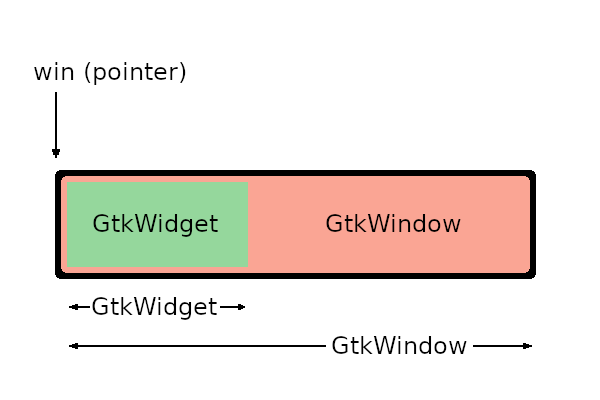
\includegraphics[width=9cm,height=6cm]{../image/window_widget.png}
\caption{GtkWindow and GtkWidget}
\end{figure}

The function \passthrough{\lstinline!gtk\_window\_new!} is defined as
follows.

\begin{lstlisting}[language=C]
GtkWidget *
gtk_window_new (void);
\end{lstlisting}

By this definition, it returns a pointer to GtkWidget, not GtkWindow. It
actually creates a new GtkWindow instance (not GtkWidget) but returns a
pointer to GtkWidget. However,the pointer points the GtkWidget and at
the same time it also points GtkWindow that contains GtkWidget in it.

If you want to use \passthrough{\lstinline!win!} as a pointer to the
GtkWindow, you need to cast it.

\begin{lstlisting}[language=C]
(GtkWindow *) win
\end{lstlisting}

Or you can use \passthrough{\lstinline!GTK\_WINDOW!} macro that performs
a similar function.

\begin{lstlisting}[language=C]
GTK_WINDOW (win)
\end{lstlisting}

This is a recommended way.

\hypertarget{connect-it-to-gtkapplication.}{%
\paragraph{Connect it to
GtkApplication.}\label{connect-it-to-gtkapplication.}}

The function \passthrough{\lstinline!gtk\_window\_set\_application!} is
used to connect GtkWindow to GtkApplication.

\begin{lstlisting}[language=C]
gtk_window_set_application (GTK_WINDOW (win), GTK_APPLICATION (app));
\end{lstlisting}

You need to cast \passthrough{\lstinline!win!} to GtkWindow and
\passthrough{\lstinline!app!} to GtkApplication.
\passthrough{\lstinline!GTK\_WINDOW!} and
\passthrough{\lstinline!GTK\_APPLICATION!} macro is appropriate for
that.

GtkApplication continues to run until the related window is destroyed.
If you didn't connect GtkWindow and GtkApplication, GtkApplication
destroys itself immediately. Because no window is connected to
GtkApplication, GtkApplication doesn't need to wait anything. As it
destroys itself, the GtkWindow is also destroyed.

\hypertarget{show-the-window.}{%
\paragraph{Show the window.}\label{show-the-window.}}

The function \passthrough{\lstinline!gtk\_widget\_show!} is used to show
the window.

Gtk4 changes the default widget visibility to on, so every widget
doesn't need this function to show itself. But, there's an exception.
Top window (this term will be explained later) isn't visible when it is
created. So you need to use the function above to show the window.

Save the program as \passthrough{\lstinline!pr3.c!} and compile and run
it.

\begin{lstlisting}
$ comp pr3
$ ./a.out
\end{lstlisting}

A small window appears.

\begin{figure}
\centering
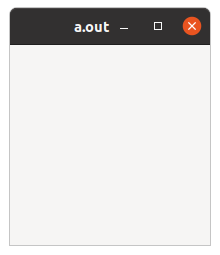
\includegraphics[width=3.3cm,height=3.825cm]{../image/screenshot_pr3.png}
\caption{Screenshot of the window}
\end{figure}

Click on the close button then the window disappears and the program
finishes.

\hypertarget{gtkapplicationwindow}{%
\subsubsection{GtkApplicationWindow}\label{gtkapplicationwindow}}

GtkApplicationWindow is a child object of GtkWindow. It has some extra
functionality for better integration with GtkApplication. It is
recommended to use it instead of GtkWindow when you use GtkApplication.

Now rewrite the program and use GtkApplicationWindow.

\begin{lstlisting}[language=C, numbers=left]
static void
app_activate (GApplication *app, gpointer user_data) {
  GtkWidget *win;

  win = gtk_application_window_new (GTK_APPLICATION (app));
  gtk_window_set_title (GTK_WINDOW (win), "pr4");
  gtk_window_set_default_size (GTK_WINDOW (win), 400, 300);
  gtk_widget_show (win);
}
\end{lstlisting}

When you create GtkApplicationWindow, you need to give GtkApplication
instance as an argument. Then it automatically connect these two
instances. So you don't need to call
\passthrough{\lstinline!gtk\_window\_set\_application!} any more.

The program sets the title and the default size of the window. Compile
it and run \passthrough{\lstinline!a.out!}, then you will see a bigger
window with its title ``pr4''.

\begin{figure}
\centering
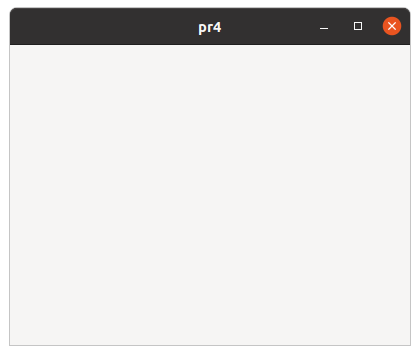
\includegraphics[width=6.3cm,height=5.325cm]{../image/screenshot_pr4.png}
\caption{Screenshot of the window}
\end{figure}

  \hypertarget{widgets-1}{%
\section{Widgets (1)}\label{widgets-1}}

\hypertarget{gtklabel-gtkbutton-and-gtkbox}{%
\subsection{GtkLabel, GtkButton and
GtkBox}\label{gtklabel-gtkbutton-and-gtkbox}}

\hypertarget{gtklabel}{%
\subsubsection{GtkLabel}\label{gtklabel}}

In the previous section we made a window and displayed it on the screen.
Now we go on to the next topic, where we add widgets to this window. The
simplest widget is GtkLabel. It is a widget with text in it.

\begin{lstlisting}[language=C, numbers=left]
#include <gtk/gtk.h>

static void
app_activate (GApplication *app, gpointer user_data) {
  GtkWidget *win;
  GtkWidget *lab;

  win = gtk_application_window_new (GTK_APPLICATION (app));
  gtk_window_set_title (GTK_WINDOW (win), "lb1");
  gtk_window_set_default_size (GTK_WINDOW (win), 400, 300);

  lab = gtk_label_new ("Hello.");
  gtk_window_set_child (GTK_WINDOW (win), lab);

  gtk_widget_show (win);
}

int
main (int argc, char **argv) {
  GtkApplication *app;
  int stat;

  app = gtk_application_new ("com.github.ToshioCP.lb1", G_APPLICATION_FLAGS_NONE);
  g_signal_connect (app, "activate", G_CALLBACK (app_activate), NULL);
  stat =g_application_run (G_APPLICATION (app), argc, argv);
  g_object_unref (app);
  return stat;
}
\end{lstlisting}

Save this program to a file \passthrough{\lstinline!lb1.c!}. Then
compile and run it.

\begin{lstlisting}
$ comp lb1
$ ./a.out
\end{lstlisting}

A window with a message ``Hello.'' appears.

\begin{figure}
\centering
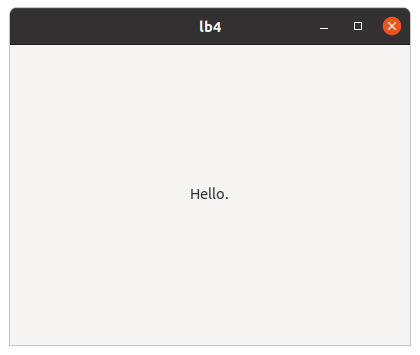
\includegraphics[width=6.3cm,height=5.325cm]{../image/screenshot_lb1.png}
\caption{Screenshot of the label}
\end{figure}

There's only a little change between \passthrough{\lstinline!pr4.c!} and
\passthrough{\lstinline!lb1.c!}. A program
\passthrough{\lstinline!diff!} is good to know the difference between
two files.

\begin{lstlisting}
$ cd misc; diff pr4.c lb1.c
5a6
>   GtkWidget *lab;
8c9
<   gtk_window_set_title (GTK_WINDOW (win), "pr4");
---
>   gtk_window_set_title (GTK_WINDOW (win), "lb1");
9a11,14
> 
>   lab = gtk_label_new ("Hello.");
>   gtk_window_set_child (GTK_WINDOW (win), lab);
> 
18c23
<   app = gtk_application_new ("com.github.ToshioCP.pr4", G_APPLICATION_FLAGS_NONE);
---
>   app = gtk_application_new ("com.github.ToshioCP.lb1", G_APPLICATION_FLAGS_NONE);
\end{lstlisting}

This tells us:

\begin{itemize}
\tightlist
\item
  The definition of a new variable \passthrough{\lstinline!lab!} is
  added.
\item
  The title of the window is changed.
\item
  A label is created and connected to the window as a child.
\end{itemize}

The function
\passthrough{\lstinline!gtk\_window\_set\_child (GTK\_WINDOW (win), lab)!}
makes the label \passthrough{\lstinline!lab!} a child widget of the
window \passthrough{\lstinline!win!}. Be careful. A child widget is
different from a child object. Objects have parent-child relationships
and widgets also have parent-child relationships. But these two
relationships are totally different. Don't be confused. In the program
\passthrough{\lstinline!lb1.c!}, \passthrough{\lstinline!lab!} is a
child widget of \passthrough{\lstinline!win!}. Child widgets are always
located in their parent widget on the screen. See how the window has
appeared on the screen. The application window includes the label.

The window \passthrough{\lstinline!win!} doesn't have any parents. We
call such a window top-level window. An application can have more than
one top-level window.

\hypertarget{gtkbutton}{%
\subsubsection{GtkButton}\label{gtkbutton}}

The next widget to introduce is GtkButton. It displays a button on the
screen with a label or icon on it. In this subsection, we will make a
button with a label. When the button is clicked, it emits a ``clicked''
signal. The following program shows how to catch the signal to then do
something.

\begin{lstlisting}[language=C, numbers=left]
#include <gtk/gtk.h>

static void
click_cb (GtkButton *btn, gpointer user_data) {
  g_print ("Clicked.\n");
}

static void
app_activate (GApplication *app, gpointer user_data) {
  GtkWidget *win;
  GtkWidget *btn;

  win = gtk_application_window_new (GTK_APPLICATION (app));
  gtk_window_set_title (GTK_WINDOW (win), "lb2");
  gtk_window_set_default_size (GTK_WINDOW (win), 400, 300);

  btn = gtk_button_new_with_label ("Click me");
  gtk_window_set_child (GTK_WINDOW (win), btn);
  g_signal_connect (btn, "clicked", G_CALLBACK (click_cb), NULL);

  gtk_widget_show (win);
}

int
main (int argc, char **argv) {
  GtkApplication *app;
  int stat;

  app = gtk_application_new ("com.github.ToshioCP.lb2", G_APPLICATION_FLAGS_NONE);
  g_signal_connect (app, "activate", G_CALLBACK (app_activate), NULL);
  stat =g_application_run (G_APPLICATION (app), argc, argv);
  g_object_unref (app);
  return stat;
}
\end{lstlisting}

Look at the line 17 to 19. First, it creates a GtkButton instance
\passthrough{\lstinline!btn!} with a label ``Click me''. Then, adds the
button to the window \passthrough{\lstinline!win!} as a child. Finally,
connects a ``clicked'' signal of the button to a handler (function)
\passthrough{\lstinline!click\_cb!}. So, if
\passthrough{\lstinline!btn!} is clicked, the function
\passthrough{\lstinline!click\_cb!} is invoked. The suffix ``cb'' means
``call back''.

Name the program \passthrough{\lstinline!lb2.c!} and save it. Now
compile and run it.

\begin{figure}
\centering
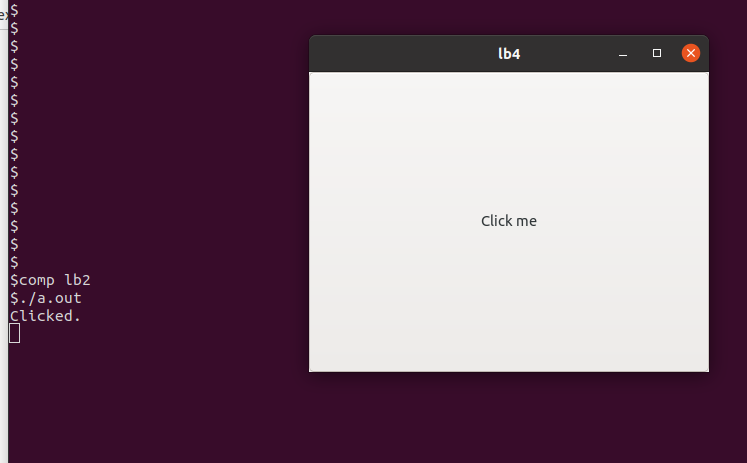
\includegraphics[width=11.205cm,height=6.945cm]{../image/screenshot_lb2.png}
\caption{Screenshot of the label}
\end{figure}

A window with the button appears. Click the button (it is a large
button, you can click everywhere in the window), then a string
``Clicked.'' appears on the terminal. It shows the handler was invoked
by clicking the button.

It's good that we make sure that the clicked signal was caught and the
handler was invoked by using \passthrough{\lstinline!g\_print!}.
However, using g\_print is out of harmony with Gtk which is a GUI
library. So, we will change the handler. The following code is
\passthrough{\lstinline!lb3.c!}.

\begin{lstlisting}[language=C, numbers=left]
static void
click_cb (GtkButton *btn, gpointer user_data) {
  GtkWindow *win = GTK_WINDOW (user_data);
  gtk_window_destroy (win);
}

static void
app_activate (GApplication *app, gpointer user_data) {
  GtkWidget *win;
  GtkWidget *btn;

  win = gtk_application_window_new (GTK_APPLICATION (app));
  gtk_window_set_title (GTK_WINDOW (win), "lb3");
  gtk_window_set_default_size (GTK_WINDOW (win), 400, 300);

  btn = gtk_button_new_with_label ("Quit");
  gtk_window_set_child (GTK_WINDOW (win), btn);
  g_signal_connect (btn, "clicked", G_CALLBACK (click_cb), win);

  gtk_widget_show (win);
}
\end{lstlisting}

And the difference between \passthrough{\lstinline!lb2.c!} and
\passthrough{\lstinline!lb3.c!} is as follows.

\begin{lstlisting}
$ cd misc; diff lb2.c lb3.c
5c5,6
<   g_print ("Clicked.\n");
---
>   GtkWindow *win = GTK_WINDOW (user_data);
>   gtk_window_destroy (win);
14c15
<   gtk_window_set_title (GTK_WINDOW (win), "lb2");
---
>   gtk_window_set_title (GTK_WINDOW (win), "lb3");
17c18
<   btn = gtk_button_new_with_label ("Click me");
---
>   btn = gtk_button_new_with_label ("Quit");
19c20
<   g_signal_connect (btn, "clicked", G_CALLBACK (click_cb), NULL);
---
>   g_signal_connect (btn, "clicked", G_CALLBACK (click_cb), win);
29c30
<   app = gtk_application_new ("com.github.ToshioCP.lb2", G_APPLICATION_FLAGS_NONE);
---
>   app = gtk_application_new ("com.github.ToshioCP.lb3", G_APPLICATION_FLAGS_NONE);
35d35
< 
\end{lstlisting}

The changes are:

\begin{itemize}
\tightlist
\item
  The function \passthrough{\lstinline!g\_print!} in
  \passthrough{\lstinline!lb2.c!} was deleted and the two lines above
  are inserted instead.
\item
  The label of \passthrough{\lstinline!btn!} is changed from ``Click
  me'' to ``Quit''.
\item
  The fourth argument of \passthrough{\lstinline!g\_signal\_connect!} is
  changed from \passthrough{\lstinline!NULL!} to
  \passthrough{\lstinline!win!}.
\end{itemize}

The most important change is the fourth argument of
\passthrough{\lstinline!g\_signal\_connect!}. This argument is described
as ``data to pass to handler'' in the definition of
\passthrough{\lstinline!g\_signal\_connect!} in
\href{https://docs.gtk.org/gobject/func.signal_connect.html}{GObject API
Reference}. Therefore, \passthrough{\lstinline!win!} which is a pointer
to GtkApplicationWindow is passed to the handler as a second parameter
\passthrough{\lstinline!user\_data!}. The handler then casts it to a
pointer to GtkWindow and calls
\passthrough{\lstinline!gtk\_window\_destroy!} to destroy the top-level
window. The application then quits.

\hypertarget{gtkbox}{%
\subsubsection{GtkBox}\label{gtkbox}}

GtkWindow and GtkApplicationWindow can have only one child. If you want
to add two or more widgets in a window, you need a container widget.
GtkBox is one of the containers. It arranges two or more child widgets
into a single row or column. The following procedure shows the way to
add two buttons in a window.

\begin{itemize}
\tightlist
\item
  Create a GtkApplicationWindow instance.
\item
  Create a GtkBox instance and add it to the GtkApplicationWindow as a
  child.
\item
  Create a GtkButton instance and append it to the GtkBox.
\item
  Create another GtkButton instance and append it to the GtkBox.
\end{itemize}

After this, the Widgets are connected as the following diagram.

\begin{figure}
\centering
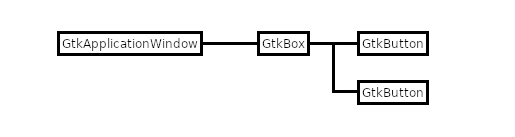
\includegraphics[width=7.725cm,height=2.055cm]{../image/box.png}
\caption{Parent-child relationship}
\end{figure}

The program \passthrough{\lstinline!lb4.c!} includes these widgets. It
is as follows.

\begin{lstlisting}[language=C, numbers=left]
#include <gtk/gtk.h>

static void
click1_cb (GtkButton *btn, gpointer user_data) {
  const gchar *s;

  s = gtk_button_get_label (btn);
  if (g_strcmp0 (s, "Hello.") == 0)
    gtk_button_set_label (btn, "Good-bye.");
  else
    gtk_button_set_label (btn, "Hello.");
}

static void
click2_cb (GtkButton *btn, gpointer user_data) {
  GtkWindow *win = GTK_WINDOW (user_data);
  gtk_window_destroy (win);
}

static void
app_activate (GApplication *app, gpointer user_data) {
  GtkWidget *win;
  GtkWidget *box;
  GtkWidget *btn1;
  GtkWidget *btn2;

  win = gtk_application_window_new (GTK_APPLICATION (app));
  gtk_window_set_title (GTK_WINDOW (win), "lb4");
  gtk_window_set_default_size (GTK_WINDOW (win), 400, 300);

  box = gtk_box_new (GTK_ORIENTATION_VERTICAL, 5);
  gtk_box_set_homogeneous (GTK_BOX (box), TRUE);
  gtk_window_set_child (GTK_WINDOW (win), box);

  btn1 = gtk_button_new_with_label ("Hello.");
  g_signal_connect (btn1, "clicked", G_CALLBACK (click1_cb), NULL);

  btn2 = gtk_button_new_with_label ("Quit");
  g_signal_connect (btn2, "clicked", G_CALLBACK (click2_cb), win);

  gtk_box_append (GTK_BOX (box), btn1);
  gtk_box_append (GTK_BOX (box), btn2);

  gtk_widget_show (win);
}

int
main (int argc, char **argv) {
  GtkApplication *app;
  int stat;

  app = gtk_application_new ("com.github.ToshioCP.lb4", G_APPLICATION_FLAGS_NONE);
  g_signal_connect (app, "activate", G_CALLBACK (app_activate), NULL);
  stat =g_application_run (G_APPLICATION (app), argc, argv);
  g_object_unref (app);
  return stat;
}
\end{lstlisting}

Look at the function \passthrough{\lstinline!app\_activate!}.

After the creation of a GtkApplicationWindow instance, a GtkBox instance
is created.

\begin{lstlisting}
box = gtk_box_new(GTK_ORIENTATION_VERTICAL, 5);
gtk_box_set_homogeneous (GTK_BOX (box), TRUE);
\end{lstlisting}

The first argument arranges the children of the box vertically. The
second argument is the size between the children. The next function
fills the box with the children, giving them the same space.

After that, two buttons \passthrough{\lstinline!btn1!} and
\passthrough{\lstinline!btn2!} are created and the signal handlers are
set. Then, these two buttons are appended to the box.

\begin{figure}
\centering
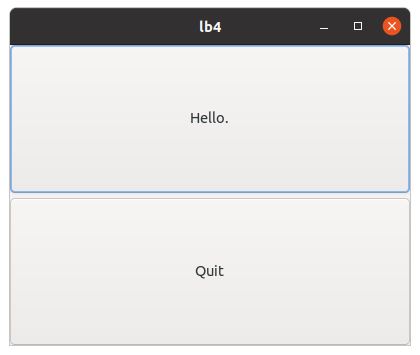
\includegraphics[width=6.3cm,height=5.325cm]{../image/screenshot_lb4.png}
\caption{Screenshot of the box}
\end{figure}

The handler corresponds to \passthrough{\lstinline!btn1!} toggles its
label. The handler corresponds to \passthrough{\lstinline!btn2!}
destroys the top-level window and the application quits.

  \hypertarget{widgets-2}{%
\section{Widgets (2)}\label{widgets-2}}

\hypertarget{gtktextview-gtktextbuffer-and-gtkscrolledwindow}{%
\subsection{GtkTextView, GtkTextBuffer and
GtkScrolledWindow}\label{gtktextview-gtktextbuffer-and-gtkscrolledwindow}}

\hypertarget{gtktextview-and-gtktextbuffer}{%
\subsubsection{GtkTextView and
GtkTextBuffer}\label{gtktextview-and-gtktextbuffer}}

GtkTextView is a widget for multi-line text editing. GtkTextBuffer is a
text buffer which is connected to GtkTextView. See the sample program
\passthrough{\lstinline!tfv1.c!} below.

\begin{lstlisting}[language=C, numbers=left]
#include <gtk/gtk.h>

static void
app_activate (GApplication *app, gpointer user_data) {
  GtkWidget *win;
  GtkWidget *tv;
  GtkTextBuffer *tb;
  gchar *text;

  text =
      "Once upon a time, there was an old man who was called Taketori-no-Okina. "
      "It is a japanese word that means a man whose work is making bamboo baskets.\n"
      "One day, he went into a mountain and found a shining bamboo. "
      "\"What a mysterious bamboo it is!,\" he said. "
      "He cut it, then there was a small cute baby girl in it. "
      "The girl was shining faintly. "
      "He thought this baby girl is a gift from Heaven and took her home.\n"
      "His wife was surprized at his tale. "
      "They were very happy because they had no children. "
      ;
  win = gtk_application_window_new (GTK_APPLICATION (app));
  gtk_window_set_title (GTK_WINDOW (win), "Taketori");
  gtk_window_set_default_size (GTK_WINDOW (win), 400, 300);

  tv = gtk_text_view_new ();
  tb = gtk_text_view_get_buffer (GTK_TEXT_VIEW (tv));
  gtk_text_buffer_set_text (tb, text, -1);
  gtk_text_view_set_wrap_mode (GTK_TEXT_VIEW (tv), GTK_WRAP_WORD_CHAR);

  gtk_window_set_child (GTK_WINDOW (win), tv);

  gtk_widget_show (win);
}

int
main (int argc, char **argv) {
  GtkApplication *app;
  int stat;

  app = gtk_application_new ("com.github.ToshioCP.tfv1", G_APPLICATION_FLAGS_NONE);
  g_signal_connect (app, "activate", G_CALLBACK (app_activate), NULL);
  stat = g_application_run (G_APPLICATION (app), argc, argv);
  g_object_unref (app);
  return stat;
}
\end{lstlisting}

Look at line 25. A GtkTextView instance is created and its pointer is
assigned to \passthrough{\lstinline!tv!}. When the GtkTextView instance
is created, a GtkTextBuffer instance is also created and connected to
the GtkTextView automatically. ``GtkTextBuffer instance'' will be
referred to simply as ``GtkTextBuffer'' or ``buffer''. In the next line,
the pointer to the buffer is got and assigned to
\passthrough{\lstinline!tb!}. Then, the text from line 10 to 20 is
assigned to the buffer.

GtkTextView has a wrap mode. When it is set to
\passthrough{\lstinline!GTK\_WRAP\_WORD\_CHAR!}, text wraps in between
words, or if that is not enough, also between graphemes.

In line 30, \passthrough{\lstinline!tv!} is added to
\passthrough{\lstinline!win!} as a child.

Now compile and run it.

\begin{figure}
\centering
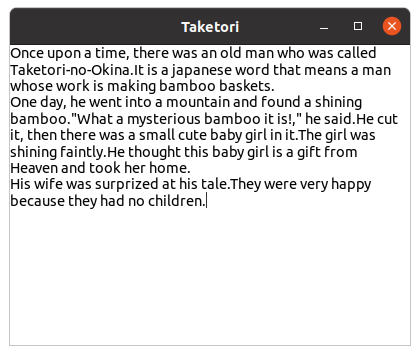
\includegraphics[width=6.3cm,height=5.325cm]{../image/screenshot_tfv1.png}
\caption{GtkTextView}
\end{figure}

There's an I-beam pointer in the window. You can add or delete any
characters on the GtkTextView, and your changes are kept in the
GtkTextBuffer. If you add more characters beyond the limit of the
window, the height increases and the window extends. If the height gets
bigger than the height of the display screen, you won't be able to
control the size of the window, and change it back to the original size.
This is a problem and shows that there is a bug in our program. This can
solve it by adding a GtkScrolledWindow between the GtkApplicationWindow
and GtkTextView.

\hypertarget{gtkscrolledwindow}{%
\subsubsection{GtkScrolledWindow}\label{gtkscrolledwindow}}

What we need to do is:

\begin{itemize}
\tightlist
\item
  Create a GtkScrolledWindow and insert it as a child of the
  GtkApplicationWindow; and
\item
  Insert the GtkTextView widget to the GtkScrolledWindow as a child.
\end{itemize}

Modify \passthrough{\lstinline!tfv1.c!} and save it as
\passthrough{\lstinline!tfv2.c!}. The difference between these two files
is small.

\begin{lstlisting}
$ cd tfv; diff tfv1.c tfv2.c
5a6
>   GtkWidget *scr;
24a26,28
>   scr = gtk_scrolled_window_new ();
>   gtk_window_set_child (GTK_WINDOW (win), scr);
> 
30c34
<   gtk_window_set_child (GTK_WINDOW (win), tv);
---
>   gtk_scrolled_window_set_child (GTK_SCROLLED_WINDOW (scr), tv);
40c44
<   app = gtk_application_new ("com.github.ToshioCP.tfv1", G_APPLICATION_FLAGS_NONE);
---
>   app = gtk_application_new ("com.github.ToshioCP.tfv2", G_APPLICATION_FLAGS_NONE);
\end{lstlisting}

Here is the complete code of \passthrough{\lstinline!tfv2.c!}.

\begin{lstlisting}[language=C, numbers=left]
#include <gtk/gtk.h>

static void
app_activate (GApplication *app, gpointer user_data) {
  GtkWidget *win;
  GtkWidget *scr;
  GtkWidget *tv;
  GtkTextBuffer *tb;
  gchar *text;

  text =
      "Once upon a time, there was an old man who was called Taketori-no-Okina. "
      "It is a japanese word that means a man whose work is making bamboo baskets.\n"
      "One day, he went into a mountain and found a shining bamboo. "
      "\"What a mysterious bamboo it is!,\" he said. "
      "He cut it, then there was a small cute baby girl in it. "
      "The girl was shining faintly. "
      "He thought this baby girl is a gift from Heaven and took her home.\n"
      "His wife was surprized at his tale. "
      "They were very happy because they had no children. "
      ;
  win = gtk_application_window_new (GTK_APPLICATION (app));
  gtk_window_set_title (GTK_WINDOW (win), "Taketori");
  gtk_window_set_default_size (GTK_WINDOW (win), 400, 300);

  scr = gtk_scrolled_window_new ();
  gtk_window_set_child (GTK_WINDOW (win), scr);

  tv = gtk_text_view_new ();
  tb = gtk_text_view_get_buffer (GTK_TEXT_VIEW (tv));
  gtk_text_buffer_set_text (tb, text, -1);
  gtk_text_view_set_wrap_mode (GTK_TEXT_VIEW (tv), GTK_WRAP_WORD_CHAR);

  gtk_scrolled_window_set_child (GTK_SCROLLED_WINDOW (scr), tv);

  gtk_widget_show (win);
}

int
main (int argc, char **argv) {
  GtkApplication *app;
  int stat;

  app = gtk_application_new ("com.github.ToshioCP.tfv2", G_APPLICATION_FLAGS_NONE);
  g_signal_connect (app, "activate", G_CALLBACK (app_activate), NULL);
  stat = g_application_run (G_APPLICATION (app), argc, argv);
  g_object_unref (app);
  return stat;
}
\end{lstlisting}

Compile and run it. Notice how this time the window doesn't extend when
you type a lot of characters, it just scrolls and displays a slider.

  \hypertarget{string-and-memory-management}{%
\section{String and memory
management}\label{string-and-memory-management}}

GtkTextView and GtkTextBuffer have functions that use string parameters
or return a string. The knowledge of strings and memory management is
useful to understand how to use these functions.

\hypertarget{string-and-memory}{%
\subsection{String and memory}\label{string-and-memory}}

A String is an array of characters that is terminated with
`\textbackslash0'. Strings are not a C type such as char, int, float or
double, but exist as a pointer to a character array. They behaves like a
string type which you may be familiar from other languages. So, this
pointer is often called `a string'.

In the following, \passthrough{\lstinline!a!} and
\passthrough{\lstinline!b!} defined as character arrays, and are
strings.

\begin{lstlisting}[language=C]
char a[10], *b;

a[0] = 'H';
a[1] = 'e';
a[2] = 'l';
a[3] = 'l';
a[4] = 'o';
a[5] = '\0';

b = a;
/* *b is 'H' */
/* *(++b) is 'e' */
\end{lstlisting}

The array \passthrough{\lstinline!a!} has \passthrough{\lstinline!char!}
elements and the size of ten. The first six elements are `H', `e', `l',
`l', `o' and `\textbackslash0'. This array represents the string
``Hello''. The first five elements are character codes that correspond
to the characters. The sixth element is `\textbackslash0', which is the
same as zero, and indicates that the string ends there. The size of the
array is 10, so 4 bytes aren't used, but that's OK, they are just
ignored.

The variable `b' is a pointer to a character. Because
\passthrough{\lstinline!b!} is assigned to be
\passthrough{\lstinline!a!}, \passthrough{\lstinline!a!} and
\passthrough{\lstinline!b!} point the same character (`H'). The variable
\passthrough{\lstinline!a!} is defined as an array and it can't be
changed. It always point the top address of the array. On the other
hand, `b' is a pointer, which is mutable, so \passthrough{\lstinline!b!}
can be change. It is then possible to write statements like
\passthrough{\lstinline!++b!}, which means take the value in b (n
address), increase it by one, and store that back in
\passthrough{\lstinline!b!}.

If a pointer is NULL, it points to nothing. So, the pointer is not a
string. A NULL string on the other hand will be a pointer which points
to a location that contains \passthrough{\lstinline!\\0!}, which is a
string of length 0 (or ""). Programs that use strings will include bugs
if you aren't careful when using NULL pointers.

Another annoying problem is the memory that a string is allocated. There
are four cases:

\begin{itemize}
\tightlist
\item
  The string is read only;
\item
  The string is in static memory area;
\item
  The string is in stack; and
\item
  The string is in memory allocated from the heap area.
\end{itemize}

\hypertarget{read-only-string}{%
\subsection{Read only string}\label{read-only-string}}

A string literal in a C program is surrounded by double quotes and
written as the following:

\begin{lstlisting}[language=C]
char *s;
s = "Hello"
\end{lstlisting}

``Hello'' is a string literal, and is stored in program memory. A string
literal is read only. In the program above, \passthrough{\lstinline!s!}
points the string literal.

So, the following program is illegal.

\begin{lstlisting}[language=C]
*(s+1) = 'a';
\end{lstlisting}

The result is undefined. Probably a bad thing will happen, for example,
a segmentation fault.

NOTE: The memory of the literal string is allocated when the program is
compiled. It is possible to view all the literal strings defined in your
program by using the \passthrough{\lstinline!string!} command.

\hypertarget{strings-defined-as-arrays}{%
\subsection{Strings defined as arrays}\label{strings-defined-as-arrays}}

If a string is defined as an array, it's in either stored in the static
memory area or stack. This depends on the class of the array. If the
array's class is \passthrough{\lstinline!static!}, then it's placed in
static memory area. This allocation and memory address is fixed for the
life of the program. This area can be changed and is writable.

If the array's class is \passthrough{\lstinline!auto!}, then it's placed
in stack. If the array is defined inside a function, its default class
is \passthrough{\lstinline!auto!}. The stack area will disappear when
the function exits and returns to the caller. Arrays defined on the
stack are writable.

\begin{lstlisting}[language=C]
static char a[] = {'H', 'e', 'l', 'l', 'o', '\0'};

void
print_strings (void) {
  char b[] = "Hello";

  a[1] = 'a'; /* Because the array is static, it's writable. */
  b[1] = 'a'; /* Because the array is auto, it's writable. */

  printf ("%s\n", a); /* Hallo */
  printf ("%s\n", b); /* Hallo */
}
\end{lstlisting}

The array \passthrough{\lstinline!a!} is defined externally to a
function and is global in its scope. Such variables are placed in static
memory area even if the \passthrough{\lstinline!static!} class is left
out. The compiler calculates the number of the elements in the right
hand side (six), and then creates code that allocates six bytes in the
static memory area and copies the data to this memory.

The array \passthrough{\lstinline!b!} is defined inside the function so
its class is \passthrough{\lstinline!auto!}. The compiler calculates the
number of the elements in the string literal. It has six elements as the
zero termination character is also included. The compiler creates code
which allocates six bytes memory in the stack and copies the data to the
memory.

Both \passthrough{\lstinline!a!} and \passthrough{\lstinline!b!} are
writable.

The memory is managed by the executable program. You don't need your
program to allocate or free the memory for \passthrough{\lstinline!a!}
and \passthrough{\lstinline!b!}. The array \passthrough{\lstinline!a!}
is created then the program is first run and remains for the life of the
program. The array \passthrough{\lstinline!b!} is created on the stack
then the function is called, disappears when the function returns.

\hypertarget{strings-in-the-heap-area}{%
\subsection{Strings in the heap area}\label{strings-in-the-heap-area}}

You can also get, use and release memory from the heap area. The
standard C library provides \passthrough{\lstinline!malloc!} to get
memory and \passthrough{\lstinline!free!} to put back memory. GLib
provides the functions \passthrough{\lstinline!g\_new!} and
\passthrough{\lstinline!g\_free!} to do the same thing, with support for
some additional Glib functionality.

\begin{lstlisting}[language=C]
g_new (struct_type, n_struct)
\end{lstlisting}

\passthrough{\lstinline!g\_new!} is a macro to allocate memory for an
array.

\begin{itemize}
\tightlist
\item
  \passthrough{\lstinline!struct\_type!} is the type of the element of
  the array.
\item
  \passthrough{\lstinline!n\_struct!} is the size of the array.
\item
  The return value is a pointer to the array. Its type is a pointer to
  \passthrough{\lstinline!struct\_type!}.
\end{itemize}

For example,

\begin{lstlisting}[language=C]
char *s;
s = g_new (char, 10);
/* s points an array of char. The size of the array is 10. */

struct tuple {int x, y;} *t;
t = g_new (struct tuple, 5);
/* t points an array of struct tuple. */
/* The size of the array is 5. */
\end{lstlisting}

\passthrough{\lstinline!g\_free!} frees memory.

\begin{lstlisting}[language=C]
void
g_free (gpointer mem);
\end{lstlisting}

If \passthrough{\lstinline!mem!} is NULL,
\passthrough{\lstinline!g\_free!} does nothing.
\passthrough{\lstinline!gpointer!} is a type of general pointer. It is
the same as \passthrough{\lstinline!void *!}. This pointer can be casted
to any pointer type. Conversely, any pointer type can be casted to
\passthrough{\lstinline!gpointer!}.

\begin{lstlisting}[language=C]
g_free (s);
/* Frees the memory allocated to s. */

g_free (t);
/* Frees the memory allocated to t. */
\end{lstlisting}

If the argument doesn't point allocated memory it will cause an error,
specifically, a segmentation fault.

Some Glib functions allocate memory. For example,
\passthrough{\lstinline!g\_strdup!} allocates memory and copies a string
given as an argument.

\begin{lstlisting}[language=C]
char *s;
s = g_strdup ("Hello");
g_free (s);
\end{lstlisting}

The string literal ``Hello'' has 6 bytes because the string has
`\textbackslash0' at the end it. \passthrough{\lstinline!g\_strdup!}
gets 6 bytes from the heap area and copies the string to the memory.
\passthrough{\lstinline!s!} is assigned the top address of the memory.
\passthrough{\lstinline!g\_free!} returns the memory to the heap area.

\passthrough{\lstinline!g\_strdup!} is described in
\href{https://docs.gtk.org/glib/func.strdup.html}{GLib API Reference}.
The following is extracted from the reference.

\begin{quote}
The returned string should be freed with
\passthrough{\lstinline!g\_free()!} when no longer needed.
\end{quote}

The function reference will describe if the returned value needs to be
freed. If you forget to free the allocated memory it will remain
allocated. Repeated use will cause more memory to be allocated to the
program, which will grow over time. This is called a memory leak, and
the only way to address this bug is to close the program (and restart
it), which will automatically release all of the programs memory back to
the system.

Some GLib functions return a string which mustn't be freed by the
caller.

\begin{lstlisting}[language=C]
const char *
g_quark_to_string (GQuark quark);
\end{lstlisting}

This function returns \passthrough{\lstinline!const char*!} type. The
qualifier \passthrough{\lstinline!const!} means that the returned value
is immutable. The characters pointed by the returned value aren't be
allowed to be changed or freed.

If a variable is qualified with \passthrough{\lstinline!const!}, the
variable can't be assigned except during initialization.

\begin{lstlisting}[language=C]
const int x = 10; /* initialization is OK. */

x = 20; /* This is illegal because x is qualified with const */
\end{lstlisting}

  \hypertarget{widgets-3}{%
\section{Widgets (3)}\label{widgets-3}}

\hypertarget{open-signal}{%
\subsection{Open signal}\label{open-signal}}

\hypertarget{g_application_handles_open-flag}{%
\subsubsection{G\_APPLICATION\_HANDLES\_OPEN
flag}\label{g_application_handles_open-flag}}

The GtkTextView, GtkTextBuffer and GtkScrolledWindow widgets have given
us a minimum editor in the previous section. We will now add a function
to read a file and rework the program into a file viewer. There are many
ways to implement the function and because this is a tutorial for
beginners, we'll take the easiest one.

When the program starts, we will give the filename to open as an
argument.

\begin{lstlisting}
$ ./a.out filename
\end{lstlisting}

It will open the file and insert its contents into the GtkTextBuffer.

To do this, we need to know how GtkApplication (or GApplication)
recognizes arguments. This is described in the
\href{https://docs.gtk.org/gio/class.Application.html}{GIO API
Reference, Application}.

When GtkApplication is created, a flag (with the type GApplicationFlags)
is provided as an argument.

\begin{lstlisting}[language=C]
GtkApplication *
gtk_application_new (const gchar *application_id, GApplicationFlags flags);
\end{lstlisting}

This tutorial explains only two flags,
\passthrough{\lstinline!G\_APPLICATION\_FLAGS\_NONE!} and
\passthrough{\lstinline!G\_APPLICATION\_HANDLES\_OPEN!}. If you want to
handle command line arguments, the
\passthrough{\lstinline!G\_APPLICATION\_HANDLES\_COMMAND\_LINE!} flag is
what you need. How to use the new application method is described in
\href{https://docs.gtk.org/gio/method.Application.run.html}{GIO API
Reference, g\_application\_run}, and the flag is described in the
\href{https://docs.gtk.org/gio/flags.ApplicationFlags.html}{GIO API
Reference, ApplicationFlags}.

\begin{lstlisting}
GApplicationFlags' Members

G_APPLICATION_FLAGS_NONE  Default. (No argument allowed)
  ... ... ...
G_APPLICATION_HANDLES_OPEN  This application handles opening files (in the primary instance).
  ... ... ...
\end{lstlisting}

There are ten flags in total, but we only need two of them so far. We've
already used \passthrough{\lstinline!G\_APPLICATION\_FLAGS\_NONE!}, as
it is the simplest option, and no arguments are allowed. If you provide
arguments when running the application, an error will occur.

The flag \passthrough{\lstinline!G\_APPLICATION\_HANDLES\_OPEN!} is the
second simplest option. It allows arguments but only files. The
application assumes all the arguments are filenames and we will use this
flag when creating our GtkApplication.

\begin{lstlisting}[language=C]
app = gtk_application_new ("com.github.ToshioCP.tfv3", G_APPLICATION_HANDLES_OPEN);
\end{lstlisting}

\hypertarget{open-signal-1}{%
\subsubsection{open signal}\label{open-signal-1}}

Now, when the application starts, two signals can be emitted.

\begin{itemize}
\tightlist
\item
  activate signal --- This signal is emitted when there's no argument.
\item
  open signal --- This signal is emitted when there is at least one
  argument.
\end{itemize}

The handler of the ``open'' signal is defined as follows.

\begin{lstlisting}[language=C]
void user_function (GApplication *application,
                   gpointer      files,
                   gint          n_files,
                   gchar        *hint,
                   gpointer      user_data)
\end{lstlisting}

The parameters are:

\begin{itemize}
\tightlist
\item
  \passthrough{\lstinline!application!} --- the application (usually
  GtkApplication)
\item
  \passthrough{\lstinline!files!} --- an array of GFiles. {[}array
  length=n\_files{]} {[}element-type GFile{]}
\item
  \passthrough{\lstinline!n\_files!} --- the number of the elements of
  \passthrough{\lstinline!files!}
\item
  \passthrough{\lstinline!hint!} --- a hint provided by the calling
  instance (usually it can be ignored)
\item
  \passthrough{\lstinline!user\_data!} --- user data set when the signal
  handler was connected.
\end{itemize}

How to read a specified file (GFile) will be described next.

\hypertarget{making-a-file-viewer}{%
\subsection{Making a file viewer}\label{making-a-file-viewer}}

\hypertarget{what-is-a-file-viewer}{%
\subsubsection{What is a file viewer?}\label{what-is-a-file-viewer}}

A file viewer is a program that displays the text file that is given as
an argument. Our file viewer will work as follows.

\begin{itemize}
\tightlist
\item
  When arguments are given, it treats the first argument as a filename
  and opens it.
\item
  If opening the file succeeds, it reads the contents of the file and
  inserts it to GtkTextBuffer and then shows the window.
\item
  If it fails to open the file, it will show an error message and quit.
\item
  If there's no argument, it will shows an error message and quit.
\item
  If there are two or more arguments, the second one and any others are
  ignored.
\end{itemize}

The program which does this is shown below.

\begin{lstlisting}[language=C, numbers=left]
#include <gtk/gtk.h>

static void
app_activate (GApplication *app, gpointer user_data) {
  g_print ("You need a filename argument.\n");
}

static void
app_open (GApplication *app, GFile ** files, gint n_files, gchar *hint, gpointer user_data) {
  GtkWidget *win;
  GtkWidget *scr;
  GtkWidget *tv;
  GtkTextBuffer *tb;
  char *contents;
  gsize length;
  char *filename;

  win = gtk_application_window_new (GTK_APPLICATION (app));
  gtk_window_set_default_size (GTK_WINDOW (win), 400, 300);

  scr = gtk_scrolled_window_new ();
  gtk_window_set_child (GTK_WINDOW (win), scr);

  tv = gtk_text_view_new ();
  tb = gtk_text_view_get_buffer (GTK_TEXT_VIEW (tv));
  gtk_text_view_set_wrap_mode (GTK_TEXT_VIEW (tv), GTK_WRAP_WORD_CHAR);
  gtk_text_view_set_editable (GTK_TEXT_VIEW (tv), FALSE);
  gtk_scrolled_window_set_child (GTK_SCROLLED_WINDOW (scr), tv);

  if (g_file_load_contents (files[0], NULL, &contents, &length, NULL, NULL)) {
    gtk_text_buffer_set_text (tb, contents, length);
    g_free (contents);
    if ((filename = g_file_get_basename (files[0])) != NULL) {
      gtk_window_set_title (GTK_WINDOW (win), filename);
      g_free (filename);
    }
    gtk_widget_show (win);
  } else {
    if ((filename = g_file_get_path (files[0])) != NULL) {
      g_print ("No such file: %s.\n", filename);
      g_free (filename);
    }
    gtk_window_destroy (GTK_WINDOW (win));
  }
}

int
main (int argc, char **argv) {
  GtkApplication *app;
  int stat;

  app = gtk_application_new ("com.github.ToshioCP.tfv3", G_APPLICATION_HANDLES_OPEN);
  g_signal_connect (app, "activate", G_CALLBACK (app_activate), NULL);
  g_signal_connect (app, "open", G_CALLBACK (app_open), NULL);
  stat = g_application_run (G_APPLICATION (app), argc, argv);
  g_object_unref (app);
  return stat;
}
\end{lstlisting}

Save it as \passthrough{\lstinline!tfv3.c!}. Then compile and run it.

\begin{lstlisting}
$ comp tfv3
$ ./a.out tfv3.c
\end{lstlisting}

\begin{figure}
\centering
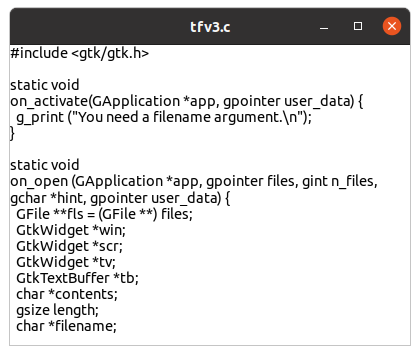
\includegraphics[width=6.3cm,height=5.325cm]{../image/screenshot_tfv3.png}
\caption{File viewer}
\end{figure}

Let's explain how the program \passthrough{\lstinline!tfv3.c!} works.
First, the function \passthrough{\lstinline!main!} has only two changes
from the previous version.

\begin{itemize}
\tightlist
\item
  \passthrough{\lstinline!G\_APPLICATION\_FLAGS\_NONE!} is replaced by
  \passthrough{\lstinline!G\_APPLICATION\_HANDLES\_OPEN!}; and
\item
  \passthrough{\lstinline!g\_signal\_connect (app, "open", G\_CALLBACK (on\_open), NULL)!}
  is added.
\end{itemize}

Next, the handler \passthrough{\lstinline!app\_activate!} is added and
is very simple. It just outputs the error message and the application
quits immediately because no window is created.

The main functionality is the in the handler
\passthrough{\lstinline!app\_open!}. It

\begin{itemize}
\tightlist
\item
  Creates GtkApplicationWindow, GtkScrolledWindow, GtkTextView and
  GtkTextBuffer and connects them together;
\item
  Sets wrap mode to \passthrough{\lstinline!GTK\_WRAP\_WORD\_CHAR!} in
  GtktextView;
\item
  Sets GtkTextView to non-editable because the program isn't an editor
  but only a viewer;
\item
  Reads the file and inserts the text into GtkTextBuffer (this will be
  explained in detail later); and
\item
  If the file is not opened then outputs an error message and destroys
  the window. This makes the application quit.
\end{itemize}

The following is the important file reading part of the program and is
shown again below.

\begin{lstlisting}[language=C]
if (g_file_load_contents (files[0], NULL, &contents, &length, NULL, NULL)) {
  gtk_text_buffer_set_text (tb, contents, length);
  g_free (contents);
  if ((filename = g_file_get_basename (files[0])) != NULL) {
    gtk_window_set_title (GTK_WINDOW (win), filename);
    g_free (filename);
  }
  gtk_widget_show (win);
} else {
  if ((filename = g_file_get_path (files[0])) != NULL) {
    g_print ("No such file: %s.\n", filename);
    g_free (filename);
  }
  gtk_window_destroy (GTK_WINDOW (win));
}
\end{lstlisting}

The function \passthrough{\lstinline!g\_file\_load\_contents!} loads the
file contents into a buffer, which is automatically allocated and sets
\passthrough{\lstinline!contents!} to point that buffer. The length of
the buffer is set to \passthrough{\lstinline!length!}. It returns
\passthrough{\lstinline!TRUE!} if the file's contents are successfully
loaded and \passthrough{\lstinline!FALSE!} if an error occurs.

If this function succeeds, it inserts the contents into GtkTextBuffer,
frees the buffer pointed by \passthrough{\lstinline!contents!}, sets the
title of the window, frees the memories pointed by
\passthrough{\lstinline!filename!} and then shows the window. If it
fails, it outputs an error message and destroys the window, causing the
program to quit.

\hypertarget{gtknotebook}{%
\subsection{GtkNotebook}\label{gtknotebook}}

GtkNotebook is a container widget that uses tabs and contains multiple
children. The child that is displayed depends on which tab has been
selected.

\begin{figure}
\centering
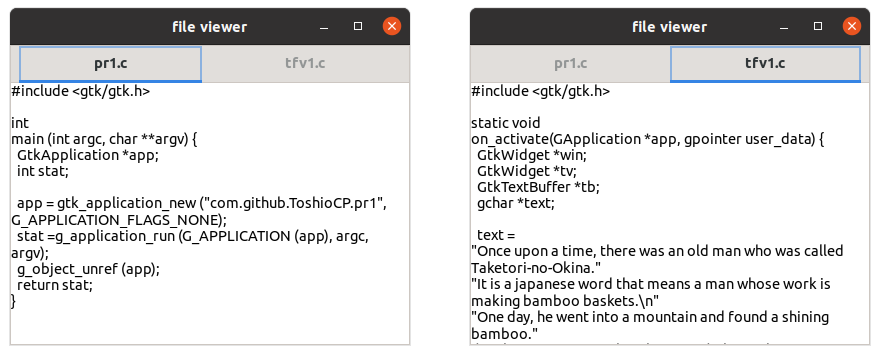
\includegraphics[width=13.2cm,height=5.325cm]{../image/screenshot_gtk_notebook.png}
\caption{GtkNotebook}
\end{figure}

Looking at the screenshots above, the left one is the window at the
startup. It shows the file \passthrough{\lstinline!pr1.c!} and the
filename is in the left tab. After clicking on the right tab, the
contents of the file \passthrough{\lstinline!tfv1.c!} are shown instead.
This is shown in the right screenshot.

The GtkNotebook widget is inserted as a child of GtkApplicationWindow
and contains a GtkScrolledWindow for each file that is being displayed.
The code to do this is given in \passthrough{\lstinline!tfv4.c!} and is:

\begin{lstlisting}[language=C, numbers=left]
#include <gtk/gtk.h>

static void
app_activate (GApplication *app, gpointer user_data) {
  g_print ("You need a filename argument.\n");
}

static void
app_open (GApplication *app, GFile ** files, gint n_files, gchar *hint, gpointer user_data) {
  GtkWidget *win;
  GtkWidget *nb;
  GtkWidget *lab;
  GtkNotebookPage *nbp;
  GtkWidget *scr;
  GtkWidget *tv;
  GtkTextBuffer *tb;
  char *contents;
  gsize length;
  char *filename;
  int i;

  win = gtk_application_window_new (GTK_APPLICATION (app));
  gtk_window_set_title (GTK_WINDOW (win), "file viewer");
  gtk_window_set_default_size (GTK_WINDOW (win), 400, 300);
  gtk_window_maximize (GTK_WINDOW (win));

  nb = gtk_notebook_new ();
  gtk_window_set_child (GTK_WINDOW (win), nb);

  for (i = 0; i < n_files; i++) {
    if (g_file_load_contents (files[i], NULL, &contents, &length, NULL, NULL)) {
      scr = gtk_scrolled_window_new ();
      tv = gtk_text_view_new ();
      tb = gtk_text_view_get_buffer (GTK_TEXT_VIEW (tv));
      gtk_text_view_set_wrap_mode (GTK_TEXT_VIEW (tv), GTK_WRAP_WORD_CHAR);
      gtk_text_view_set_editable (GTK_TEXT_VIEW (tv), FALSE);
      gtk_scrolled_window_set_child (GTK_SCROLLED_WINDOW (scr), tv);

      gtk_text_buffer_set_text (tb, contents, length);
      g_free (contents);
      if ((filename = g_file_get_basename (files[i])) != NULL) {
        lab = gtk_label_new (filename);
        g_free (filename);
      } else
        lab = gtk_label_new ("");
      gtk_notebook_append_page (GTK_NOTEBOOK (nb), scr, lab);
      nbp = gtk_notebook_get_page (GTK_NOTEBOOK (nb), scr);
      g_object_set (nbp, "tab-expand", TRUE, NULL);
    } else if ((filename = g_file_get_path (files[i])) != NULL) {
        g_print ("No such file: %s.\n", filename);
        g_free (filename);
    } else
        g_print ("No valid file is given\n");
  }
  if (gtk_notebook_get_n_pages (GTK_NOTEBOOK (nb)) > 0)
    gtk_widget_show (win);
  else
    gtk_window_destroy (GTK_WINDOW (win));
}

int
main (int argc, char **argv) {
  GtkApplication *app;
  int stat;

  app = gtk_application_new ("com.github.ToshioCP.tfv4", G_APPLICATION_HANDLES_OPEN);
  g_signal_connect (app, "activate", G_CALLBACK (app_activate), NULL);
  g_signal_connect (app, "open", G_CALLBACK (app_open), NULL);
  stat = g_application_run (G_APPLICATION (app), argc, argv);
  g_object_unref (app);
  return stat;
}
\end{lstlisting}

Most of the changes are in the function
\passthrough{\lstinline!app\_open!}. The numbers at the left of the
following items are line numbers in the source code.

\begin{itemize}
\tightlist
\item
  11-13: Variables \passthrough{\lstinline!nb!},
  \passthrough{\lstinline!lab!} and \passthrough{\lstinline!nbp!} are
  defined and will point to a new GtkNotebook, GtkLabel and
  GtkNotebookPage widget respectively.
\item
  23: The window's title is set to ``file viewer''.
\item
  25: The size of the window is set to maximum because a big window is
  appropriate for file viewers.
\item
  27-28 GtkNotebook is created and inserted to the GtkApplicationWindow
  as a child.
\item
  30-59 For-loop. Each loop corresponds to a filename argument, and
  \passthrough{\lstinline!files[i]!} is GFile object containing the i-th
  argument.
\item
  32-37 GtkScrollledWindow, GtkTextView are created and GtkTextBuffer
  found from the new GtkTextView. GtkTextView is connected to
  GtkScrolledWindow as a child. Each file gets their own copy of these
  widgets, so they are created inside the for-loop.
\item
  39-40 inserts the contents of the file into GtkTextBuffer and frees
  the memory pointed by \passthrough{\lstinline!contents!}.
\item
  41-43: Gets the filename and creates GtkLabel with the filename and
  then frees \passthrough{\lstinline!filename!}.
\item
  44-45: If \passthrough{\lstinline!filename!} is NULL, creates GtkLabel
  with the empty string.
\item
  46: Appends GtkScrolledWindow as a page, with the tab GtkLabel, to
  GtkNotebook. At this time a GtkNoteBookPage widget is created
  automatically. The GtkScrolledWindow widget is connected to the
  GtkNotebookPage. Therefore, the structure is like this:
\end{itemize}

\begin{lstlisting}
    GtkNotebook -- GtkNotebookPage -- GtkScrolledWindow
\end{lstlisting}

\begin{itemize}
\tightlist
\item
  47: Gets GtkNotebookPage widget and sets \passthrough{\lstinline!nbp!}
  to point to this GtkNotebookPage.
\item
  48: GtkNotebookPage has a property set called ``tab-expand''. If it is
  set to TRUE then the tab expands horizontally as long as possible. If
  it is FALSE, then the width of the tab is determined by the size of
  the label. \passthrough{\lstinline!g\_object\_set!} is a general
  function to set properties in objects. See
  \href{https://docs.gtk.org/gobject/method.Object.set.html}{GObject API
  Reference, g\_object\_set}.
\item
  49-51: If the file cannot be read, ``No such file'' message is
  displayed and the \passthrough{\lstinline!filename!} buffer is freed.
\item
  52-53: If \passthrough{\lstinline!filename!} is NULL, the ``No valid
  file is given'' message is outputted.
\item
  55-58: If at least one file was read, then the number of
  GtkNotebookPage is greater than zero. If it's true, it shows the
  window. If it's false, it destroys the window, which causes the
  program to quit.
\end{itemize}

  \hypertarget{defining-a-child-object}{%
\section{Defining a Child object}\label{defining-a-child-object}}

\hypertarget{a-very-simple-editor}{%
\subsection{A Very Simple Editor}\label{a-very-simple-editor}}

In the previous section we made a very simple file viewer. Now we go on
to rewrite it and turn it into very simple editor. Its source file is in
tfe1.c (text file editor 1).

GtkTextView has a feature for editing multiple lines. Therefore, we
don't need to write the program from scratch, we just add two things to
the file viewer:

\begin{itemize}
\tightlist
\item
  Memory to store a pointer to the GFile instance.
\item
  A function to write the file.
\end{itemize}

There are a couple of ways to store the details of GFile.

\begin{itemize}
\tightlist
\item
  Use global variables; or
\item
  Make a child object, which can extend the instance memory for the
  GFile object.
\end{itemize}

Using global variables is easy to implement. Define a sufficient size
array of pointers to GFile. For example,

\begin{lstlisting}[language=C]
GFile *f[20];
\end{lstlisting}

The variable \passthrough{\lstinline!f[i]!} corresponds to the file
associated to the i-th GtkNotebookPage. There are however two problems
with this. The first concerns the size of the array. If a user gives too
many arguments (more than 20 in the example above), it is impossible to
store the additional pointers to the GFile instances. The second is the
increasing difficulty for maintenance of the program. We have a small
program so far, but however, if you continue developing it, the size of
the program will grow. Generally speaking, the bigger the program size,
the more difficult it is to keep track of and maintain global variables.
Global variables can be used and changed anywhere throughout the entire
program.

Making a child object is a good idea in terms of maintenance. One thing
you need to be careful of is the difference between ``child object'' and
``child widget''. Here we are describing a ``child object''. A child
object includes, and expands on its parent object, as a child object
derives everything from the parent object.

\begin{figure}
\centering
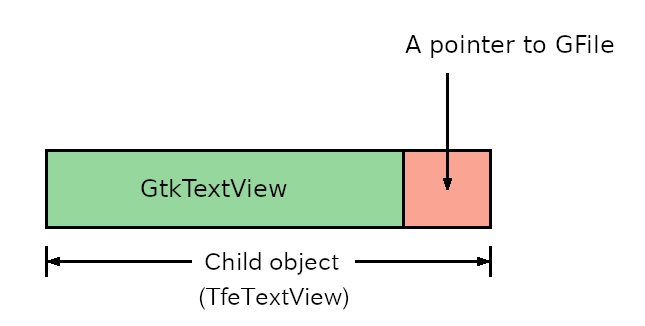
\includegraphics[width=9.675cm,height=4.89cm]{../image/child.png}
\caption{Child object of GtkTextView}
\end{figure}

We will define TfeTextView as a child object of GtkTextView. It has
everything that GtkTextView has. Specifically, TfeTextView has a
GtkTextbuffer which corresponds to the GtkTextView inside TfeTextView.
The additional important thing is that TfeTextView can also keep an
additional pointer to GFile.

In general, this is how GObjects work. Understanding the general theory
about Gobject's is difficult, particularly for beginners. So, I will
just show you the way how to write the code and avoid the theoretical
side. If you want to know about GObject system, refer to another
\href{https://github.com/ToshioCP/Gobject-tutorial}{tutorial}.

\hypertarget{how-to-define-a-child-object-of-gtktextview}{%
\subsection{How to Define a Child Object of
GtkTextView}\label{how-to-define-a-child-object-of-gtktextview}}

Let's define the TfeTextView object, which is a child object of
GtkTextView. First, look at the program below.

\begin{lstlisting}[language=C]
#define TFE_TYPE_TEXT_VIEW tfe_text_view_get_type ()
G_DECLARE_FINAL_TYPE (TfeTextView, tfe_text_view, TFE, TEXT_VIEW, GtkTextView)

struct _TfeTextView
{
  GtkTextView parent;
  GFile *file;
};

G_DEFINE_TYPE (TfeTextView, tfe_text_view, GTK_TYPE_TEXT_VIEW);

static void
tfe_text_view_init (TfeTextView *tv) {
}

static void
tfe_text_view_class_init (TfeTextViewClass *class) {
}

void
tfe_text_view_set_file (TfeTextView *tv, GFile *f) {
  tv -> file = f;
}

GFile *
tfe_text_view_get_file (TfeTextView *tv) {
  return tv -> file;
}

GtkWidget *
tfe_text_view_new (void) {
  return GTK_WIDGET (g_object_new (TFE_TYPE_TEXT_VIEW, NULL));
}
\end{lstlisting}

If you are curious about the background theory of this program, that's
good, because knowing the theory is very important if you want to
program GTK applications. Look at
\href{https://docs.gtk.org/gobject/}{GObject API Reference}. All you
need is described there, or refer to
\href{https://github.com/ToshioCP/Gobject-tutorial}{GObject tutorial}.
It's a tough journey especially for beginners so for now, you don't need
to know about this difficult theory. It is enough to just remember the
instructions below.

\begin{itemize}
\tightlist
\item
  TfeTextView is divided into two parts. Tfe and TextView. Tfe is called
  the prefix, namespace or module. TextView is called the object.
\item
  There are three differnet identifier patterns. TfeTextView (camel
  case), tfe\_text\_view (this is used to write functions) and
  TFE\_TEXT\_VIEW (This is used to cast a pointer to point TfeTextView
  type).
\item
  First, define TFE\_TYPE\_TEXT\_VIEW macro as
  tfe\_text\_view\_get\_type (). The name is always
  (prefix)\_TYPE\_(object) and the letters are upper case. And the
  replacement text is always (prefix)\_(object)\_get\_type () and the
  letters are lower case.
\item
  Next, use G\_DECLARE\_FINAL\_TYPE macro. The arguments are the child
  object name in camel case, lower case with underscore, prefix (upper
  case), object (upper case with underscore) and parent object name
  (camel case).
\item
  Declare the structure \_TfeTextView. The underscore is necessary. The
  first member is the parent object. Notice this is not a pointer but
  the object itself. The second member and after are members of the
  child object. TfeTextView structure has a pointer to a GFile instance
  as a member.
\item
  Use G\_DEFINE\_TYPE macro. The arguments are the child object name in
  camel case, lower case with underscore and parent object type
  (prefix)\_TYPE\_(module).
\item
  Define instance init function (tfe\_text\_view\_init). Usually you
  don't need to do anything.
\item
  Define class init function (tfe\_text\_view\_class\_init). You don't
  need to do anything in this object.
\item
  Write function codes you want to add (tfe\_text\_view\_set\_file and
  tfe\_text\_view\_get\_file). \passthrough{\lstinline!tv!} is a pointer
  to the TfeTextView object instance which is a C-structure declared
  with the tag \_TfeTextView. So, the structure has a member
  \passthrough{\lstinline!file!} as a pointer to a GFile instance.
  \passthrough{\lstinline!tv->file = f!} is an assignment of
  \passthrough{\lstinline!f!} to a member \passthrough{\lstinline!file!}
  of the structure pointed by \passthrough{\lstinline!tv!}. This is an
  example how to use the extended memory in a child widget.
\item
  Write a function to create an instance. Its name is
  (prefix)\_(object)\_new. If the parent object function needs
  parameters, this function also need them. You sometimes might want to
  add some parameters. It's your choice. Use g\_object\_new function to
  create the instance. The arguments are (prefix)\_TYPE\_(object), a
  list to initialize properties and NULL. In this code no property needs
  to be initialized. And the return value is casted to GtkWidget.
\end{itemize}

This program is not perfect. It has some problems. It will be modified
later.

\hypertarget{close-request-signal}{%
\subsection{Close-request signal}\label{close-request-signal}}

Imagine that you are using this editor. First, you run the editor with
arguments. The arguments are filenames. The editor reads the files and
shows the window with the text of files in it. Then you edit the text.
After you finish editing, you exit the editor. The editor updates files
just before the window closes.

GtkWindow emits the ``close-request'' signal before it closes. We
connect the signal and the handler
\passthrough{\lstinline!before\_close!}. A handler is a C function. When
a function is connected to a certain signal, we call it a handler. The
function \passthrough{\lstinline!before\_close!} is invoked when the
signal ``close-request'' is emitted.

\begin{lstlisting}[language=C]
g_signal_connect (win, "close-request", G_CALLBACK (before_close), NULL);
\end{lstlisting}

The argument \passthrough{\lstinline!win!} is a GtkApplicationWindow, in
which the signal ``close-request'' is defined, and
\passthrough{\lstinline!before\_close!} is the handler.
\passthrough{\lstinline!G\_CALLBACK!} cast is necessary for the handler.
The program of \passthrough{\lstinline!before\_close!} is as follows.

\begin{lstlisting}[language=C, numbers=left]
static gboolean
before_close (GtkWindow *win, gpointer user_data) {
  GtkWidget *nb = GTK_WIDGET (user_data);
  GtkWidget *scr;
  GtkWidget *tv;
  GFile *file;
  char *pathname;
  GtkTextBuffer *tb;
  GtkTextIter start_iter;
  GtkTextIter end_iter;
  char *contents;
  unsigned int n;
  unsigned int i;

  n = gtk_notebook_get_n_pages (GTK_NOTEBOOK (nb));
  for (i = 0; i < n; ++i) {
    scr = gtk_notebook_get_nth_page (GTK_NOTEBOOK (nb), i);
    tv = gtk_scrolled_window_get_child (GTK_SCROLLED_WINDOW (scr));
    file = tfe_text_view_get_file (TFE_TEXT_VIEW (tv));
    tb = gtk_text_view_get_buffer (GTK_TEXT_VIEW (tv));
    gtk_text_buffer_get_bounds (tb, &start_iter, &end_iter);
    contents = gtk_text_buffer_get_text (tb, &start_iter, &end_iter, FALSE);
    if (! g_file_replace_contents (file, contents, strlen (contents), NULL, TRUE, G_FILE_CREATE_NONE, NULL, NULL, NULL)) {
      pathname = g_file_get_path (file);
      g_print ("ERROR : Can't save %s.", pathname);
      g_free (pathname);
    }
    g_free (contents);
  }
  return FALSE;
}
\end{lstlisting}

The numbers on the left of items are line numbers in the source code.

\begin{itemize}
\tightlist
\item
  15: Gets the number of pages \passthrough{\lstinline!nb!} has.
\item
  16-29: For loop with regard to the index to each pages.
\item
  17-19: Gets GtkScrolledWindow, TfeTextView and a pointer to GFile. The
  pointer was stored when \passthrough{\lstinline!app\_open!} handler
  had run. It will be shown later.
\item
  20-22: Gets GtkTextBuffer and contents.
  \passthrough{\lstinline!start\_iter!} and
  \passthrough{\lstinline!end\_iter!} are iterators of the buffer. I
  don't want to explain them now because it would take a lot of time.
  Just remember these lines for the present.
\item
  23-27: Writes the contents to the file. If it fails, it outputs an
  error message.
\item
  28: Frees \passthrough{\lstinline!contents!}.
\end{itemize}

\hypertarget{source-code-of-tfe1.c}{%
\subsection{Source code of tfe1.c}\label{source-code-of-tfe1.c}}

The following is the complete source code of
\passthrough{\lstinline!tfe1.c!}.

\begin{lstlisting}[language=C, numbers=left]
#include <gtk/gtk.h>

/* Define TfeTextView Widget which is the child object of GtkTextView */

#define TFE_TYPE_TEXT_VIEW tfe_text_view_get_type ()
G_DECLARE_FINAL_TYPE (TfeTextView, tfe_text_view, TFE, TEXT_VIEW, GtkTextView)

struct _TfeTextView
{
  GtkTextView parent;
  GFile *file;
};

G_DEFINE_TYPE (TfeTextView, tfe_text_view, GTK_TYPE_TEXT_VIEW);

static void
tfe_text_view_init (TfeTextView *tv) {
}

static void
tfe_text_view_class_init (TfeTextViewClass *class) {
}

void
tfe_text_view_set_file (TfeTextView *tv, GFile *f) {
  tv -> file = f;
}

GFile *
tfe_text_view_get_file (TfeTextView *tv) {
  return tv -> file;
}

GtkWidget *
tfe_text_view_new (void) {
  return GTK_WIDGET (g_object_new (TFE_TYPE_TEXT_VIEW, NULL));
}

/* ---------- end of the definition of TfeTextView ---------- */

static gboolean
before_close (GtkWindow *win, gpointer user_data) {
  GtkWidget *nb = GTK_WIDGET (user_data);
  GtkWidget *scr;
  GtkWidget *tv;
  GFile *file;
  char *pathname;
  GtkTextBuffer *tb;
  GtkTextIter start_iter;
  GtkTextIter end_iter;
  char *contents;
  unsigned int n;
  unsigned int i;

  n = gtk_notebook_get_n_pages (GTK_NOTEBOOK (nb));
  for (i = 0; i < n; ++i) {
    scr = gtk_notebook_get_nth_page (GTK_NOTEBOOK (nb), i);
    tv = gtk_scrolled_window_get_child (GTK_SCROLLED_WINDOW (scr));
    file = tfe_text_view_get_file (TFE_TEXT_VIEW (tv));
    tb = gtk_text_view_get_buffer (GTK_TEXT_VIEW (tv));
    gtk_text_buffer_get_bounds (tb, &start_iter, &end_iter);
    contents = gtk_text_buffer_get_text (tb, &start_iter, &end_iter, FALSE);
    if (! g_file_replace_contents (file, contents, strlen (contents), NULL, TRUE, G_FILE_CREATE_NONE, NULL, NULL, NULL)) {
      pathname = g_file_get_path (file);
      g_print ("ERROR : Can't save %s.", pathname);
      g_free (pathname);
    }
    g_free (contents);
  }
  return FALSE;
}

static void
app_activate (GApplication *app, gpointer user_data) {
  g_print ("You need to give filenames as arguments.\n");
}

static void
app_open (GApplication *app, GFile ** files, gint n_files, gchar *hint, gpointer user_data) {
  GtkWidget *win;
  GtkWidget *nb;
  GtkWidget *lab;
  GtkNotebookPage *nbp;
  GtkWidget *scr;
  GtkWidget *tv;
  GtkTextBuffer *tb;
  char *contents;
  gsize length;
  char *filename;
  int i;

  win = gtk_application_window_new (GTK_APPLICATION (app));
  gtk_window_set_title (GTK_WINDOW (win), "file editor");
  gtk_window_maximize (GTK_WINDOW (win));

  nb = gtk_notebook_new ();
  gtk_window_set_child (GTK_WINDOW (win), nb);

  for (i = 0; i < n_files; i++) {
    if (g_file_load_contents (files[i], NULL, &contents, &length, NULL, NULL)) {
      scr = gtk_scrolled_window_new ();
      tv = tfe_text_view_new ();
      tb = gtk_text_view_get_buffer (GTK_TEXT_VIEW (tv));
      gtk_text_view_set_wrap_mode (GTK_TEXT_VIEW (tv), GTK_WRAP_WORD_CHAR);
      gtk_scrolled_window_set_child (GTK_SCROLLED_WINDOW (scr), tv);

      tfe_text_view_set_file (TFE_TEXT_VIEW (tv),  g_file_dup (files[i]));
      gtk_text_buffer_set_text (tb, contents, length);
      g_free (contents);
      filename = g_file_get_basename (files[i]);
      lab = gtk_label_new (filename);
      gtk_notebook_append_page (GTK_NOTEBOOK (nb), scr, lab);
      nbp = gtk_notebook_get_page (GTK_NOTEBOOK (nb), scr);
      g_object_set (nbp, "tab-expand", TRUE, NULL);
      g_free (filename);
    } else if ((filename = g_file_get_path (files[i])) != NULL) {
        g_print ("No such file: %s.\n", filename);
        g_free (filename);
    } else
        g_print ("No valid file is given\n");
  }
  if (gtk_notebook_get_n_pages (GTK_NOTEBOOK (nb)) > 0) {
    g_signal_connect (win, "close-request", G_CALLBACK (before_close), nb);
    gtk_widget_show (win);
  } else
    gtk_window_destroy (GTK_WINDOW (win));
}

int
main (int argc, char **argv) {
  GtkApplication *app;
  int stat;

  app = gtk_application_new ("com.github.ToshioCP.tfe1", G_APPLICATION_HANDLES_OPEN);
  g_signal_connect (app, "activate", G_CALLBACK (app_activate), NULL);
  g_signal_connect (app, "open", G_CALLBACK (app_open), NULL);
  stat =g_application_run (G_APPLICATION (app), argc, argv);
  g_object_unref (app);
  return stat;
}
\end{lstlisting}

\begin{itemize}
\tightlist
\item
  107: Sets the pointer to GFile into TfeTextView.
  \passthrough{\lstinline!files[i]!} is a pointer to GFile structure. It
  will be freed by the system. So you need to copy it.
  \passthrough{\lstinline!g\_file\_dup!} duplicates the given GFile
  structure.
\item
  123: Connects ``close-request'' signal and
  \passthrough{\lstinline!before\_close!} handler. The fourth argument
  is called user data and it is given to the signal handler. So,
  \passthrough{\lstinline!nb!} is given to
  \passthrough{\lstinline!before\_close!} as the second argument.
\end{itemize}

Now compile and run it. There's a sample file in the directory
\passthrough{\lstinline!tfe!}. Type
\passthrough{\lstinline!./a.out taketori.txt!}. Modify the contents and
close the window. Make sure that the file is modified.

Now we got a very simple editor. It's not smart. We need more features
like open, save, saveas, change font and so on. We will add them in the
next section and after.

  \hypertarget{the-user-interface-ui-file-and-gtkbuilder}{%
\section{The User Interface (UI) file and
GtkBuilder}\label{the-user-interface-ui-file-and-gtkbuilder}}

\hypertarget{new-open-and-save-button}{%
\subsection{New, Open and Save button}\label{new-open-and-save-button}}

In the last section we made the almost simplest editor possible. It
reads files in the \passthrough{\lstinline!app\_open!} function at
start-up and writes them out when closing the window. It works but is
not very good. It would be better if we had ``New'', ``Open'', ``Save''
and ``Close'' buttons. This section describes how to put those buttons
into the window. Signals and handlers will be explained later.

\begin{figure}
\centering
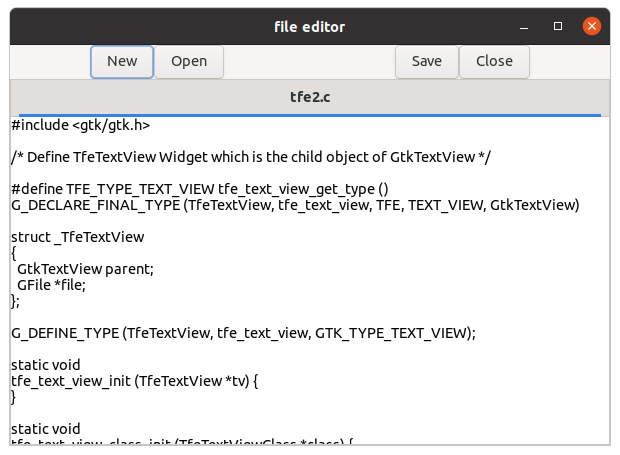
\includegraphics[width=9.3cm,height=6.825cm]{../image/screenshot_tfe2.png}
\caption{Screenshot of the file editor}
\end{figure}

The screenshot above shows the layout. The function
\passthrough{\lstinline!app\_open!} in the source code
\passthrough{\lstinline!tfe2.c!} is as follows.

\begin{lstlisting}[language=C, numbers=left]
static void
app_open (GApplication *app, GFile ** files, gint n_files, gchar *hint, gpointer user_data) {
  GtkWidget *win;
  GtkWidget *nb;
  GtkWidget *lab;
  GtkNotebookPage *nbp;
  GtkWidget *scr;
  GtkWidget *tv;
  GtkTextBuffer *tb;
  char *contents;
  gsize length;
  char *filename;
  int i;

  GtkWidget *boxv;
  GtkWidget *boxh;
  GtkWidget *dmy1;
  GtkWidget *dmy2;
  GtkWidget *dmy3;
  GtkWidget *btnn; /* button for new */
  GtkWidget *btno; /* button for open */
  GtkWidget *btns; /* button for save */
  GtkWidget *btnc; /* button for close */

  win = gtk_application_window_new (GTK_APPLICATION (app));
  gtk_window_set_title (GTK_WINDOW (win), "file editor");
  gtk_window_set_default_size (GTK_WINDOW (win), 600, 400);

  boxv = gtk_box_new (GTK_ORIENTATION_VERTICAL, 0);
  gtk_window_set_child (GTK_WINDOW (win), boxv);

  boxh = gtk_box_new (GTK_ORIENTATION_HORIZONTAL, 0);
  gtk_box_append (GTK_BOX (boxv), boxh);

  dmy1 = gtk_label_new(NULL); /* dummy label for left space */
  gtk_label_set_width_chars (GTK_LABEL (dmy1), 10);
  dmy2 = gtk_label_new(NULL); /* dummy label for center space */
  gtk_widget_set_hexpand (dmy2, TRUE);
  dmy3 = gtk_label_new(NULL); /* dummy label for right space */
  gtk_label_set_width_chars (GTK_LABEL (dmy3), 10);
  btnn = gtk_button_new_with_label ("New");
  btno = gtk_button_new_with_label ("Open");
  btns = gtk_button_new_with_label ("Save");
  btnc = gtk_button_new_with_label ("Close");

  gtk_box_append (GTK_BOX (boxh), dmy1);
  gtk_box_append (GTK_BOX (boxh), btnn);
  gtk_box_append (GTK_BOX (boxh), btno);
  gtk_box_append (GTK_BOX (boxh), dmy2);
  gtk_box_append (GTK_BOX (boxh), btns);
  gtk_box_append (GTK_BOX (boxh), btnc);
  gtk_box_append (GTK_BOX (boxh), dmy3);

  nb = gtk_notebook_new ();
  gtk_widget_set_hexpand (nb, TRUE);
  gtk_widget_set_vexpand (nb, TRUE);
  gtk_box_append (GTK_BOX (boxv), nb);

  for (i = 0; i < n_files; i++) {
    if (g_file_load_contents (files[i], NULL, &contents, &length, NULL, NULL)) {
      scr = gtk_scrolled_window_new ();
      tv = tfe_text_view_new ();
      tb = gtk_text_view_get_buffer (GTK_TEXT_VIEW (tv));
      gtk_text_view_set_wrap_mode (GTK_TEXT_VIEW (tv), GTK_WRAP_WORD_CHAR);
      gtk_scrolled_window_set_child (GTK_SCROLLED_WINDOW (scr), tv);

      tfe_text_view_set_file (TFE_TEXT_VIEW (tv),  g_file_dup (files[i]));
      gtk_text_buffer_set_text (tb, contents, length);
      g_free (contents);
      filename = g_file_get_basename (files[i]);
      lab = gtk_label_new (filename);
      gtk_notebook_append_page (GTK_NOTEBOOK (nb), scr, lab);
      nbp = gtk_notebook_get_page (GTK_NOTEBOOK (nb), scr);
      g_object_set (nbp, "tab-expand", TRUE, NULL);
      g_free (filename);
    } else if ((filename = g_file_get_path (files[i])) != NULL) {
        g_print ("No such file: %s.\n", filename);
        g_free (filename);
    } else
        g_print ("No valid file is given\n");
  }
  if (gtk_notebook_get_n_pages (GTK_NOTEBOOK (nb)) > 0) {
    gtk_widget_show (win);
  } else
    gtk_window_destroy (GTK_WINDOW (win));
}
\end{lstlisting}

The aim is to build the widgets of the main application window.

\begin{itemize}
\tightlist
\item
  25-27: Creates a GtkApplicationWindow instance and sets the title and
  default size.
\item
  29-30: Creates a GtkBox instance \passthrough{\lstinline!boxv!}. It is
  a vertical box and a child of GtkApplicationWindow. It has two
  children. The first child is a horizontal box. The second child is a
  GtkNotebook.
\item
  32-33: Creates a GtkBox instance \passthrough{\lstinline!boxh!} and
  appends it to \passthrough{\lstinline!boxv!} as a first child.
\item
  35-40: Creates three dummy labels. The labels
  \passthrough{\lstinline!dmy1!} and \passthrough{\lstinline!dmy3!} has
  a character width of ten. The other label
  \passthrough{\lstinline!dmy2!} has hexpand property which is set to be
  TRUE. This makes the label expands horizontally as long as possible.
\item
  41-44: Creates four buttons.
\item
  46-52: Appends these GtkLabel and GtkButton to
  \passthrough{\lstinline!boxh!}.
\item
  54-57: Creates a GtkNotebook instance and sets hexpand and vexpand
  properties TRUE. This makes it expand horizontally and vertically as
  big as possible. It is appended to \passthrough{\lstinline!boxv!} as
  the second child.
\end{itemize}

The number of lines to build the widgets is 33(=57-25+1). We also needed
many additional variables (\passthrough{\lstinline!boxv!},
\passthrough{\lstinline!boxh!}, \passthrough{\lstinline!dmy1!}, \ldots),
most of which weren't necessary, except for building the widgets. Are
there any good solution to reduce these work?

Gtk provides GtkBuilder. It reads user interface (UI) data and builds a
window. It reduces this cumbersome work.

\hypertarget{the-ui-file}{%
\subsection{The UI File}\label{the-ui-file}}

First, let's look at the UI file \passthrough{\lstinline!tfe3.ui!} that
is used to define the widget structure.

\begin{lstlisting}[language=XML, numbers=left]
<?xml version="1.0" encoding="UTF-8"?>
<interface>
  <object class="GtkApplicationWindow" id="win">
    <property name="title">file editor</property>
    <property name="default-width">600</property>
    <property name="default-height">400</property>
    <child>
      <object class="GtkBox" id="boxv">
        <property name="orientation">GTK_ORIENTATION_VERTICAL</property>
        <child>
          <object class="GtkBox" id="boxh">
            <property name="orientation">GTK_ORIENTATION_HORIZONTAL</property>
            <child>
              <object class="GtkLabel" id="dmy1">
                <property name="width-chars">10</property>
              </object>
            </child>
            <child>
              <object class="GtkButton" id="btnn">
                <property name="label">New</property>
              </object>
            </child>
            <child>
              <object class="GtkButton" id="btno">
                <property name="label">Open</property>
              </object>
            </child>
            <child>
              <object class="GtkLabel" id="dmy2">
                <property name="hexpand">TRUE</property>
              </object>
            </child>
            <child>
              <object class="GtkButton" id="btns">
                <property name="label">Save</property>
              </object>
            </child>
            <child>
              <object class="GtkButton" id="btnc">
                <property name="label">Close</property>
              </object>
            </child>
            <child>
              <object class="GtkLabel" id="dmy3">
                <property name="width-chars">10</property>
              </object>
            </child>
          </object>
        </child>
        <child>
          <object class="GtkNotebook" id="nb">
            <property name="hexpand">TRUE</property>
            <property name="vexpand">TRUE</property>
          </object>
        </child>
      </object>
    </child>
  </object>
</interface>
\end{lstlisting}

The structure of this file is XML. Constructs that begin with
\passthrough{\lstinline!<!} and end with \passthrough{\lstinline!>!} are
called tags. There are two types of tags, the start tag and the end tag.
For example, \passthrough{\lstinline!<interface>!} is a start tag and
\passthrough{\lstinline!</interface>!} is an end tag. The UI file begins
and ends with interface tags. Some tags, for example object tags, can
have a class and id attributes in their start tag.

\begin{itemize}
\tightlist
\item
  1: The first line is XML declaration. It specifies that the version of
  XML is 1.0 and the encoding is UTF-8. Even if the line is left out,
  GtkBuilder builds objects from the ui file. But ui files must use
  UTF-8 encoding, or GtkBuilder can't recognize it and a fatal error
  occurs.
\item
  3-6: An object with \passthrough{\lstinline!GtkApplicationWindow!}
  class and \passthrough{\lstinline!win!} id is defined. This is the top
  level window. And the three properties of the window are defined.
  \passthrough{\lstinline!title!} property is ``file editor'',
  \passthrough{\lstinline!default-width!} property is 600 and
  \passthrough{\lstinline!default-height!} property is 400.
\item
  7: child tag means a child of the widget above. For example, line 7
  tells us that GtkBox object which id is ``boxv'' is a child widget of
  \passthrough{\lstinline!win!}.
\end{itemize}

Compare this ui file and the lines 25-57 in the source code of
\passthrough{\lstinline!app\_open!} function. Those two describe the
same structure of widgets.

You can check the ui file with
\passthrough{\lstinline!gtk4-builder-tool!}.

\begin{itemize}
\tightlist
\item
  \passthrough{\lstinline!gtk4-builder-tool validate <ui file name>!}
  validates the ui file. If the ui file includes some syntactical error,
  \passthrough{\lstinline!gtk4-builder-tool!} prints the error.
\item
  \passthrough{\lstinline!gtk4-builder-tool simplify <ui file name>!}
  simplifies the ui file and prints the result. If
  \passthrough{\lstinline!--replace!} option is given, it replaces the
  ui file with the simplified one. If the ui file specifies a value of
  property but it is default, then it will be removed. And some values
  are simplified. For example, ``TRUE''and ``FALSE'' becomes ``1'' and
  ``0'' respectively. However, ``TRUE'' or ``FALSE'' is better for
  maintenance.
\end{itemize}

It is a good idea to check your ui file before compiling.

\hypertarget{gtkbuilder}{%
\subsection{GtkBuilder}\label{gtkbuilder}}

GtkBuilder builds widgets based on the ui file.

\begin{lstlisting}[language=C]
GtkBuilder *build;

build = gtk_builder_new_from_file ("tfe3.ui");
win = GTK_WIDGET (gtk_builder_get_object (build, "win"));
gtk_window_set_application (GTK_WINDOW (win), GTK_APPLICATION (app));
nb = GTK_WIDGET (gtk_builder_get_object (build, "nb"));
\end{lstlisting}

The function \passthrough{\lstinline!gtk\_builder\_new\_from\_file!}
reads the file given as an argument. Then, it builds the widgets and
creates GtkBuilder object. The function
\passthrough{\lstinline!gtk\_builder\_get\_object (build, "win")!}
returns the pointer to the widget \passthrough{\lstinline!win!}, which
is the id in the ui file. All the widgets are connected based on the
parent-children relationship described in the ui file. We only need
\passthrough{\lstinline!win!} and \passthrough{\lstinline!nb!} for the
program after this, so we don't need to take out any other widgets. This
reduces lines in the C source file.

\begin{lstlisting}
$ cd tfe; diff tfe2.c tfe3.c
58a59
>   GtkBuilder *build;
60,103c61,65
<   GtkWidget *boxv;
<   GtkWidget *boxh;
<   GtkWidget *dmy1;
<   GtkWidget *dmy2;
<   GtkWidget *dmy3;
<   GtkWidget *btnn; /* button for new */
<   GtkWidget *btno; /* button for open */
<   GtkWidget *btns; /* button for save */
<   GtkWidget *btnc; /* button for close */
< 
<   win = gtk_application_window_new (GTK_APPLICATION (app));
<   gtk_window_set_title (GTK_WINDOW (win), "file editor");
<   gtk_window_set_default_size (GTK_WINDOW (win), 600, 400);
< 
<   boxv = gtk_box_new (GTK_ORIENTATION_VERTICAL, 0);
<   gtk_window_set_child (GTK_WINDOW (win), boxv);
< 
<   boxh = gtk_box_new (GTK_ORIENTATION_HORIZONTAL, 0);
<   gtk_box_append (GTK_BOX (boxv), boxh);
< 
<   dmy1 = gtk_label_new(NULL); /* dummy label for left space */
<   gtk_label_set_width_chars (GTK_LABEL (dmy1), 10);
<   dmy2 = gtk_label_new(NULL); /* dummy label for center space */
<   gtk_widget_set_hexpand (dmy2, TRUE);
<   dmy3 = gtk_label_new(NULL); /* dummy label for right space */
<   gtk_label_set_width_chars (GTK_LABEL (dmy3), 10);
<   btnn = gtk_button_new_with_label ("New");
<   btno = gtk_button_new_with_label ("Open");
<   btns = gtk_button_new_with_label ("Save");
<   btnc = gtk_button_new_with_label ("Close");
< 
<   gtk_box_append (GTK_BOX (boxh), dmy1);
<   gtk_box_append (GTK_BOX (boxh), btnn);
<   gtk_box_append (GTK_BOX (boxh), btno);
<   gtk_box_append (GTK_BOX (boxh), dmy2);
<   gtk_box_append (GTK_BOX (boxh), btns);
<   gtk_box_append (GTK_BOX (boxh), btnc);
<   gtk_box_append (GTK_BOX (boxh), dmy3);
< 
<   nb = gtk_notebook_new ();
<   gtk_widget_set_hexpand (nb, TRUE);
<   gtk_widget_set_vexpand (nb, TRUE);
<   gtk_box_append (GTK_BOX (boxv), nb);
< 
---
>   build = gtk_builder_new_from_file ("tfe3.ui");
>   win = GTK_WIDGET (gtk_builder_get_object (build, "win"));
>   gtk_window_set_application (GTK_WINDOW (win), GTK_APPLICATION (app));
>   nb = GTK_WIDGET (gtk_builder_get_object (build, "nb"));
>   g_object_unref(build);
138c100
<   app = gtk_application_new ("com.github.ToshioCP.tfe2", G_APPLICATION_HANDLES_OPEN);
---
>   app = gtk_application_new ("com.github.ToshioCP.tfe3", G_APPLICATION_HANDLES_OPEN);
\end{lstlisting}

\passthrough{\lstinline!60,103c61,65!} means 44 (=103-60+1) lines are
changed to 5 (=65-61+1) lines. Therefore, 39 lines are reduced. Using ui
file not only shortens C source files, but also makes the widgets'
structure clear.

Now I'll show you \passthrough{\lstinline!app\_open!} function in the C
file \passthrough{\lstinline!tfe3.c!}.

\begin{lstlisting}[language=C, numbers=left]
static void
app_open (GApplication *app, GFile ** files, gint n_files, gchar *hint, gpointer user_data) {
  GtkWidget *win;
  GtkWidget *nb;
  GtkWidget *lab;
  GtkNotebookPage *nbp;
  GtkWidget *scr;
  GtkWidget *tv;
  GtkTextBuffer *tb;
  char *contents;
  gsize length;
  char *filename;
  int i;
  GtkBuilder *build;

  build = gtk_builder_new_from_file ("tfe3.ui");
  win = GTK_WIDGET (gtk_builder_get_object (build, "win"));
  gtk_window_set_application (GTK_WINDOW (win), GTK_APPLICATION (app));
  nb = GTK_WIDGET (gtk_builder_get_object (build, "nb"));
  g_object_unref(build);
  for (i = 0; i < n_files; i++) {
    if (g_file_load_contents (files[i], NULL, &contents, &length, NULL, NULL)) {
      scr = gtk_scrolled_window_new ();
      tv = tfe_text_view_new ();
      tb = gtk_text_view_get_buffer (GTK_TEXT_VIEW (tv));
      gtk_text_view_set_wrap_mode (GTK_TEXT_VIEW (tv), GTK_WRAP_WORD_CHAR);
      gtk_scrolled_window_set_child (GTK_SCROLLED_WINDOW (scr), tv);

      tfe_text_view_set_file (TFE_TEXT_VIEW (tv),  g_file_dup (files[i]));
      gtk_text_buffer_set_text (tb, contents, length);
      g_free (contents);
      filename = g_file_get_basename (files[i]);
      lab = gtk_label_new (filename);
      gtk_notebook_append_page (GTK_NOTEBOOK (nb), scr, lab);
      nbp = gtk_notebook_get_page (GTK_NOTEBOOK (nb), scr);
      g_object_set (nbp, "tab-expand", TRUE, NULL);
      g_free (filename);
    } else if ((filename = g_file_get_path (files[i])) != NULL) {
        g_print ("No such file: %s.\n", filename);
        g_free (filename);
    } else
        g_print ("No valid file is given\n");
  }
  if (gtk_notebook_get_n_pages (GTK_NOTEBOOK (nb)) > 0) {
    gtk_widget_show (win);
  } else
    gtk_window_destroy (GTK_WINDOW (win));
}
\end{lstlisting}

The whole source code of \passthrough{\lstinline!tfe3.c!} is stored in
src/tfe directory. If you want to see it, click the link above.

\hypertarget{using-ui-string}{%
\subsubsection{Using ui string}\label{using-ui-string}}

GtkBuilder can build widgets using string. Use the function
\passthrough{\lstinline!gtk\_builder\_new\_from\_string!} instead of
\passthrough{\lstinline!gtk\_builder\_new\_from\_file!}.

\begin{lstlisting}[language=C]
char *uistring;

uistring =
"<interface>"
  "<object class="GtkApplicationWindow" id="win">"
    "<property name=\"title\">file editor</property>"
    "<property name=\"default-width\">600</property>"
    "<property name=\"default-height\">400</property>"
    "<child>"
      "<object class=\"GtkBox\" id=\"boxv\">"
        "<property name="orientation">GTK_ORIENTATION_VERTICAL</property>"
... ... ...
... ... ...
"</interface>";

build = gtk_builder_new_from_stringfile (uistring);
\end{lstlisting}

This method has an advantage and disadvantage. The advantage is that the
ui string is written in the source code. So ui file is not necessary on
runtime. The disadvantage is that writing C string is a bit bothersome
because of the double quotes. If you want to use this method, you should
write a script that transforms ui file into C-string.

\begin{itemize}
\tightlist
\item
  Add backslash before each double quote.
\item
  Add double quotes at the left and right of the string in each line.
\end{itemize}

\hypertarget{using-gresource}{%
\subsubsection{Using Gresource}\label{using-gresource}}

Using Gresource is similar to using string. But Gresource is compressed
binary data, not text data. And there's a compiler that compiles ui file
into Gresource. It can compile not only text files but also binary files
such as images, sounds and so on. And after compilation, it bundles them
up into one Gresource object.

An xml file is necessary for the resource compiler
\passthrough{\lstinline!glib-compile-resources!}. It describes resource
files.

\begin{lstlisting}[language=XML, numbers=left]
<?xml version="1.0" encoding="UTF-8"?>
<gresources>
  <gresource prefix="/com/github/ToshioCP/tfe3">
    <file>tfe3.ui</file>
  </gresource>
</gresources>
\end{lstlisting}

\begin{itemize}
\tightlist
\item
  2: \passthrough{\lstinline!gresources!} tag can include multiple
  gresources (gresource tags). However, this xml has only one gresource.
\item
  3: The gresource has a prefix
  \passthrough{\lstinline!/com/github/ToshioCP/tfe3!}.
\item
  4: The gresource has \passthrough{\lstinline!tfe3.ui!}. And it is
  pointed by \passthrough{\lstinline!/com/github/ToshioCP/tfe3/tfe3.ui!}
  because it needs prefix. If you want to add more files, then insert
  them between line 4 and 5.
\end{itemize}

Save this xml text to \passthrough{\lstinline!tfe3.gresource.xml!}. The
gresource compiler \passthrough{\lstinline!glib-compile-resources!}
shows its usage with the argument \passthrough{\lstinline!--help!}.

\begin{lstlisting}
$ LANG=C glib-compile-resources --help
Usage:
  glib-compile-resources [OPTION?] FILE

Compile a resource specification into a resource file.
Resource specification files have the extension .gresource.xml,
and the resource file have the extension called .gresource.

Help Options:
  -h, --help                   Show help options

Application Options:
  --version                    Show program version and exit
  --target=FILE                Name of the output file
  --sourcedir=DIRECTORY        The directories to load files referenced in FILE from (default: current directory)
  --generate                   Generate output in the format selected for by the target filename extension
  --generate-header            Generate source header
  --generate-source            Generate source code used to link in the resource file into your code
  --generate-dependencies      Generate dependency list
  --dependency-file=FILE       Name of the dependency file to generate
  --generate-phony-targets     Include phony targets in the generated dependency file
  --manual-register            Don?t automatically create and register resource
  --internal                   Don?t export functions; declare them G_GNUC_INTERNAL
  --external-data              Don?t embed resource data in the C file; assume it's linked externally instead
  --c-name                     C identifier name used for the generated source code
  -C, --compiler               The target C compiler (default: the CC environment variable)
\end{lstlisting}

Now run the compiler.

\begin{lstlisting}
$ glib-compile-resources tfe3.gresource.xml --target=resources.c --generate-source
\end{lstlisting}

Then a C source file \passthrough{\lstinline!resources.c!} is generated.
Modify \passthrough{\lstinline!tfe3.c!} and save it as
\passthrough{\lstinline!tfe3\_r.c!}.

\begin{lstlisting}[language=C]
#include "resources.c"
... ... ...
... ... ...
build = gtk_builder_new_from_resource ("/com/github/ToshioCP/tfe3/tfe3.ui");
... ... ...
... ... ...
\end{lstlisting}

Then, compile and run it. The window appears and it is the same as the
screenshot at the beginning of this page.

  \hypertarget{build-system}{%
\section{Build system}\label{build-system}}

\hypertarget{what-do-we-need-to-think-about-to-manage-big-source-files}{%
\subsection{What do we need to think about to manage big source
files?}\label{what-do-we-need-to-think-about-to-manage-big-source-files}}

We've compiled a small editor so far. But Some bad signs are beginning
to appear.

\begin{itemize}
\tightlist
\item
  We've had only one C source file and put everything into it. We need
  to sort it out.
\item
  There are two compilers, \passthrough{\lstinline!gcc!} and
  \passthrough{\lstinline!glib-compile-resources!}. We should control
  them by one building tool.
\end{itemize}

These ideas are useful to manage big source files.

\hypertarget{divide-a-c-source-file-into-two-parts.}{%
\subsection{Divide a C source file into two
parts.}\label{divide-a-c-source-file-into-two-parts.}}

When you divide C source file into several parts, each file should
contain only one thing. For example, our source has two things, the
definition of TfeTextView and functions related to GtkApplication and
GtkApplicationWindow. It is a good idea to separate them into two files,
\passthrough{\lstinline!tfetextview.c!} and
\passthrough{\lstinline!tfe.c!}.

\begin{itemize}
\tightlist
\item
  \passthrough{\lstinline!tfetextview.c!} includes the definition and
  functions of TfeTextView.
\item
  \passthrough{\lstinline!tfe.c!} includes functions like
  \passthrough{\lstinline!main!},
  \passthrough{\lstinline!app\_activate!},
  \passthrough{\lstinline!app\_open!} and so on, which relate to
  GtkApplication and GtkApplicationWindow
\end{itemize}

Now we have three source files, \passthrough{\lstinline!tfetextview.c!},
\passthrough{\lstinline!tfe.c!} and \passthrough{\lstinline!tfe3.ui!}.
The \passthrough{\lstinline!3!} of \passthrough{\lstinline!tfe3.ui!} is
like a version number. Managing version with filenames is one possible
idea but it may make bothersome problem. You need to rewrite filename in
each version and it affects to contents of source files that refer to
filenames. So, we should take \passthrough{\lstinline!3!} away from the
filename.

In \passthrough{\lstinline!tfe.c!} the function
\passthrough{\lstinline!tfe\_text\_view\_new!} is invoked to create a
TfeTextView instance. But it is defined in
\passthrough{\lstinline!tfetextview.c!}, not
\passthrough{\lstinline!tfe.c!}. The lack of the declaration (not
definition) of \passthrough{\lstinline!tfe\_text\_view\_new!} makes
error when \passthrough{\lstinline!tfe.c!} is compiled. The declaration
is necessary in \passthrough{\lstinline!tfe.c!}. Those public
information is usually written in header files. It has
\passthrough{\lstinline!.h!} suffix like
\passthrough{\lstinline!tfetextview.h!} And header files are included by
C source files. For example, \passthrough{\lstinline!tfetextview.h!} is
included by \passthrough{\lstinline!tfe.c!}.

All the source files are listed below.

\passthrough{\lstinline!tfetextview.h!}

\begin{lstlisting}[language=C, numbers=left]
#include <gtk/gtk.h>

#define TFE_TYPE_TEXT_VIEW tfe_text_view_get_type ()
G_DECLARE_FINAL_TYPE (TfeTextView, tfe_text_view, TFE, TEXT_VIEW, GtkTextView)

void
tfe_text_view_set_file (TfeTextView *tv, GFile *f);

GFile *
tfe_text_view_get_file (TfeTextView *tv);

GtkWidget *
tfe_text_view_new (void);
\end{lstlisting}

\passthrough{\lstinline!tfetextview.c!}

\begin{lstlisting}[language=C, numbers=left]
#include <gtk/gtk.h>
#include "tfetextview.h"

struct _TfeTextView
{
  GtkTextView parent;
  GFile *file;
};

G_DEFINE_TYPE (TfeTextView, tfe_text_view, GTK_TYPE_TEXT_VIEW);

static void
tfe_text_view_init (TfeTextView *tv) {
}

static void
tfe_text_view_class_init (TfeTextViewClass *class) {
}

void
tfe_text_view_set_file (TfeTextView *tv, GFile *f) {
  tv -> file = f;
}

GFile *
tfe_text_view_get_file (TfeTextView *tv) {
  return tv -> file;
}

GtkWidget *
tfe_text_view_new (void) {
  return GTK_WIDGET (g_object_new (TFE_TYPE_TEXT_VIEW, NULL));
}
\end{lstlisting}

\passthrough{\lstinline!tfe.c!}

\begin{lstlisting}[language=C, numbers=left]
#include <gtk/gtk.h>
#include "tfetextview.h"

static void
app_activate (GApplication *app, gpointer user_data) {
  g_print ("You need a filename argument.\n");
}

static void
app_open (GApplication *app, GFile ** files, gint n_files, gchar *hint, gpointer user_data) {
  GtkWidget *win;
  GtkWidget *nb;
  GtkWidget *lab;
  GtkNotebookPage *nbp;
  GtkWidget *scr;
  GtkWidget *tv;
  GtkTextBuffer *tb;
  char *contents;
  gsize length;
  char *filename;
  int i;
  GtkBuilder *build;

  build = gtk_builder_new_from_resource ("/com/github/ToshioCP/tfe3/tfe.ui");
  win = GTK_WIDGET (gtk_builder_get_object (build, "win"));
  gtk_window_set_application (GTK_WINDOW (win), GTK_APPLICATION (app));
  nb = GTK_WIDGET (gtk_builder_get_object (build, "nb"));
  g_object_unref (build);
  for (i = 0; i < n_files; i++) {
    if (g_file_load_contents (files[i], NULL, &contents, &length, NULL, NULL)) {
      scr = gtk_scrolled_window_new ();
      tv = tfe_text_view_new ();
      tb = gtk_text_view_get_buffer (GTK_TEXT_VIEW (tv));
      gtk_text_view_set_wrap_mode (GTK_TEXT_VIEW (tv), GTK_WRAP_WORD_CHAR);
      gtk_scrolled_window_set_child (GTK_SCROLLED_WINDOW (scr), tv);

      tfe_text_view_set_file (TFE_TEXT_VIEW (tv),  g_file_dup (files[i]));
      gtk_text_buffer_set_text (tb, contents, length);
      g_free (contents);
      filename = g_file_get_basename (files[i]);
      lab = gtk_label_new (filename);
      gtk_notebook_append_page (GTK_NOTEBOOK (nb), scr, lab);
      nbp = gtk_notebook_get_page (GTK_NOTEBOOK (nb), scr);
      g_object_set (nbp, "tab-expand", TRUE, NULL);
      g_free (filename);
    } else if ((filename = g_file_get_path (files[i])) != NULL) {
        g_print ("No such file: %s.\n", filename);
        g_free (filename);
    } else
        g_print ("No valid file is given\n");
  }
  if (gtk_notebook_get_n_pages (GTK_NOTEBOOK (nb)) > 0) {
    gtk_widget_show (win);
  } else
    gtk_window_destroy (GTK_WINDOW (win));
}

int
main (int argc, char **argv) {
  GtkApplication *app;
  int stat;

  app = gtk_application_new ("com.github.ToshioCP.tfe", G_APPLICATION_HANDLES_OPEN);
  g_signal_connect (app, "activate", G_CALLBACK (app_activate), NULL);
  g_signal_connect (app, "open", G_CALLBACK (app_open), NULL);
  stat =g_application_run (G_APPLICATION (app), argc, argv);
  g_object_unref (app);
  return stat;
}
\end{lstlisting}

The ui file \passthrough{\lstinline!tfe.ui!} is the same as
\passthrough{\lstinline!tfe3.ui!} in the previous section.

\passthrough{\lstinline!tfe.gresource.xml!}

\begin{lstlisting}[language=XML, numbers=left]
<?xml version="1.0" encoding="UTF-8"?>
<gresources>
  <gresource prefix="/com/github/ToshioCP/tfe3">
    <file>tfe.ui</file>
  </gresource>
</gresources>
\end{lstlisting}

\hypertarget{make}{%
\subsection{Make}\label{make}}

Dividing a file makes it easy to maintain source files. But now we are
faced with a new problem. The building step increases.

\begin{itemize}
\tightlist
\item
  Compiling the ui file \passthrough{\lstinline!tfe.ui!} into
  \passthrough{\lstinline!resources.c!}.
\item
  Compiling \passthrough{\lstinline!tfe.c!} into
  \passthrough{\lstinline!tfe.o!} (object file).
\item
  Compiling \passthrough{\lstinline!tfetextview.c!} into
  \passthrough{\lstinline!tfetextview.o!}.
\item
  Compiling \passthrough{\lstinline!resources.c!} into
  \passthrough{\lstinline!resources.o!}.
\item
  Linking all the object files into application
  \passthrough{\lstinline!tfe!}.
\end{itemize}

Now build tool is necessary to manage it. Make is one of the build
tools. It was created in 1976. It is an old and widely used program.

Make analyzes Makefile and executes compilers. All instructions are
written in Makefile.

\begin{lstlisting}[language=make]
sample.o: sample.c
    gcc -o sample.o sample.c
\end{lstlisting}

The sample of Malefile above consists of three elements,
\passthrough{\lstinline!sample.o!}, \passthrough{\lstinline!sample.c!}
and \passthrough{\lstinline!gcc -o sample.o sample.c!}.

\begin{itemize}
\tightlist
\item
  \passthrough{\lstinline!sample.o!} is called target.
\item
  \passthrough{\lstinline!sample.c!} is prerequisite.
\item
  \passthrough{\lstinline!gcc -o sample.o sample.c!} is recipe. Recipes
  follow tab characters, not spaces. (It is very important. Use tab not
  space, or make won't work as you expected).
\end{itemize}

The rule is:

If a prerequisite modified later than a target, then make executes the
recipe.

In the example above, if \passthrough{\lstinline!sample.c!} is modified
after the generation of \passthrough{\lstinline!sample.o!}, then make
executes gcc and compile \passthrough{\lstinline!sample.c!} into
\passthrough{\lstinline!sample.o!}. If the modification time of
\passthrough{\lstinline!sample.c!} is older then the generation of
\passthrough{\lstinline!sample.o!}, then no compiling is necessary, so
make does nothing.

The Makefile for \passthrough{\lstinline!tfe!} is as follows.

\begin{lstlisting}[language=make, numbers=left]
all: tfe

tfe: tfe.o tfetextview.o resources.o
    gcc -o tfe tfe.o tfetextview.o resources.o `pkg-config --libs gtk4`

tfe.o: tfe.c tfetextview.h
    gcc -c -o tfe.o `pkg-config --cflags gtk4` tfe.c
tfetextview.o: tfetextview.c tfetextview.h
    gcc -c -o tfetextview.o `pkg-config --cflags gtk4` tfetextview.c
resources.o: resources.c
    gcc -c -o resources.o `pkg-config --cflags gtk4` resources.c

resources.c: tfe.gresource.xml tfe.ui
    glib-compile-resources tfe.gresource.xml --target=resources.c --generate-source

.Phony: clean

clean:
    rm -f tfe tfe.o tfetextview.o resources.o resources.c
\end{lstlisting}

You only need to type \passthrough{\lstinline!make!}.

\begin{lstlisting}
$ make
gcc -c -o tfe.o `pkg-config --cflags gtk4` tfe.c
gcc -c -o tfetextview.o `pkg-config --cflags gtk4` tfetextview.c
glib-compile-resources tfe.gresource.xml --target=resources.c --generate-source
gcc -c -o resources.o `pkg-config --cflags gtk4` resources.c
gcc -o tfe tfe.o tfetextview.o resources.o `pkg-config --libs gtk4`
\end{lstlisting}

I used only very basic rules to write this Makefile. There are many more
convenient methods to make it more compact. But it will be long to
explain it. So I want to finish explaining make and move on to the next
topic.

\hypertarget{rake}{%
\subsection{Rake}\label{rake}}

Rake is a similar program to make. It is written in Ruby code. If you
don't use Ruby, you don't need to read this subsection. However, Ruby is
really sophisticated and recommendable script language.

\begin{itemize}
\tightlist
\item
  Rakefile controls the behavior of \passthrough{\lstinline!rake!}.
\item
  You can write any Ruby code in Rakefile.
\end{itemize}

Rake has task and file task, which is similar to target, prerequisite
and recipe in make.

\begin{lstlisting}[language=Ruby, numbers=left]
require 'rake/clean'

targetfile = "tfe"
srcfiles = FileList["tfe.c", "tfetextview.c", "resources.c"]
rscfile = srcfiles[2]
objfiles = srcfiles.gsub(/.c$/, '.o')

CLEAN.include(targetfile, objfiles, rscfile)

task default: targetfile

file targetfile => objfiles do |t|
  sh "gcc -o #{t.name} #{t.prerequisites.join(' ')} `pkg-config --libs gtk4`"
end

objfiles.each do |obj|
  src = obj.gsub(/.o$/,'.c')
  file obj => src do |t|
    sh "gcc -c -o #{t.name} `pkg-config --cflags gtk4` #{t.source}"
  end
end

file rscfile => ["tfe.gresource.xml", "tfe.ui"] do |t|
  sh "glib-compile-resources #{t.prerequisites[0]} --target=#{t.name} --generate-source"
end
\end{lstlisting}

The contents of the \passthrough{\lstinline!Rakefile!} is almost same as
the \passthrough{\lstinline!Makefile!} in the previous subsection.

\begin{itemize}
\tightlist
\item
  3-6: Defines target file, source file and so on.
\item
  1, 8: Loads clean library. And defines CLEAN file list. The files
  included by CLEAN will be removed when
  \passthrough{\lstinline!rake clean!} is typed on the command line.
\item
  10: The default target depends on
  \passthrough{\lstinline!targetfile!}. The task
  \passthrough{\lstinline!default!} is the final goal of tasks.
\item
  12-14: \passthrough{\lstinline!targetfile!} depends on
  \passthrough{\lstinline!objfiles!}. The variable
  \passthrough{\lstinline!t!} is a task object.

  \begin{itemize}
  \tightlist
  \item
    \passthrough{\lstinline!t.name!} is a target name
  \item
    \passthrough{\lstinline!t.prerequisites!} is an array of
    prerequisites.
  \item
    \passthrough{\lstinline!t.source!} is the first element of
    prerequisites.
  \end{itemize}
\item
  \passthrough{\lstinline!sh!} is a method to give the following string
  to shell as an argument and executes the shell.
\item
  16-21: There's a loop by each element of the array of
  \passthrough{\lstinline!objfiles!}. Each object depends on
  corresponding source file.
\item
  23-25: Resource file depends on xml file and ui file.
\end{itemize}

Rakefile might seem to be difficult for beginners. But, you can use any
Ruby syntax in Rakefile, so it is really flexible. If you practice Ruby
and Rakefile, it will be highly productive tools.

\hypertarget{meson-and-ninja}{%
\subsection{Meson and ninja}\label{meson-and-ninja}}

Meson is one of the most popular building tool despite the developing
version. And ninja is similar to make but much faster than make. Several
years ago, most of the C developers used autotools and make. But now the
situation has changed. Many developers are using meson and ninja now.

To use meson, you first need to write
\passthrough{\lstinline!meson.build!} file.

\begin{lstlisting}[numbers=left]
project('tfe', 'c')

gtkdep = dependency('gtk4')

gnome=import('gnome')
resources = gnome.compile_resources('resources','tfe.gresource.xml')

sourcefiles=files('tfe.c', 'tfetextview.c')

executable('tfe', sourcefiles, resources, dependencies: gtkdep)
\end{lstlisting}

\begin{itemize}
\tightlist
\item
  1: The function \passthrough{\lstinline!project!} defines things about
  the project. The first parameter is the name of the project and the
  second is the programming language.
\item
  2: \passthrough{\lstinline!dependency!} function defines a dependency
  that is taken by \passthrough{\lstinline!pkg-config!}. We put
  \passthrough{\lstinline!gtk4!} as an argument.
\item
  5: \passthrough{\lstinline!import!} function imports a module. In line
  5, the gnome module is imported and assigned to the variable
  \passthrough{\lstinline!gnome!}. The gnome module provides helper
  tools to build GTK programs.
\item
  6: \passthrough{\lstinline!.compile\_resources!} is a method of the
  gnome module and compiles files to resources under the instruction of
  xml file. In line 6, the resource filename is
  \passthrough{\lstinline!resources!}, which means
  \passthrough{\lstinline!resources.c!} and
  \passthrough{\lstinline!resources.h!}, and xml file is
  \passthrough{\lstinline!tfe.gresource.xml!}. This method generates C
  source file by default.
\item
  8: Defines source files.
\item
  10: Executable function generates a target file by compiling source
  files. The first parameter is the filename of the target. The
  following parameters are source files. The last parameter is an option
  \passthrough{\lstinline!dependencies!}.
  \passthrough{\lstinline!gtkdep!} is used in the compilation.
\end{itemize}

Now run meson and ninja.

\begin{lstlisting}
$ meson _build
$ ninja -C _build
\end{lstlisting}

Then, the executable file \passthrough{\lstinline!tfe!} is generated
under the directory \passthrough{\lstinline!\_build!}.

\begin{lstlisting}
$ _build/tfe tfe.c tfetextview.c
\end{lstlisting}

Then the window appears. And two notebook pages are in the window. One
notebook is \passthrough{\lstinline!tfe.c!} and the other is
\passthrough{\lstinline!tfetextview.c!}.

I've shown you three build tools. I think meson and ninja is the best
choice for the present.

We divided a file into some categorized files and used a build tool.
This method is used by many developers.

  \hypertarget{initialization-and-destruction-of-instances}{%
\section{Initialization and destruction of
instances}\label{initialization-and-destruction-of-instances}}

A new version of the text file editor (\passthrough{\lstinline!tfe!})
will be made in this section and the following four sections. It is
\passthrough{\lstinline!tfe5!}. There are many changes from the prior
version. All the sources are listed in Section 16. They are located in
two directories, src/tfe5 and src/tfetextview.

\hypertarget{encapsulation}{%
\subsection{Encapsulation}\label{encapsulation}}

We've divided C source file into two parts. But it is not enough in
terms of encapsulation.

\begin{itemize}
\tightlist
\item
  \passthrough{\lstinline!tfe.c!} includes everything other than
  TfeTextView. It should be divided at least into two parts,
  \passthrough{\lstinline!tfeapplication.c!} and
  \passthrough{\lstinline!tfenotebook.c!}.
\item
  Header files also need to be organized.
\end{itemize}

However, first of all, I'd like to focus on the object TfeTextView. It
is a child object of GtkTextView and has a new member
\passthrough{\lstinline!file!} in it. The important thing is to manage
the Gfile object pointed by \passthrough{\lstinline!file!}.

\begin{itemize}
\tightlist
\item
  What is necessary to GFile when creating (or initializing)
  TfeTextView?
\item
  What is necessary to GFile when destructing TfeTextView?
\item
  TfeTextView should read/write a file by itself or not?
\item
  How it communicates with objects outside?
\end{itemize}

You need to know at least class, instance and signals before thinking
about them. I will explain them in this section and the next section.
After that I will explain:

\begin{itemize}
\tightlist
\item
  Organizing functions.
\item
  How to use GtkFileChooserDialog
\end{itemize}

\hypertarget{gobject-and-its-children}{%
\subsection{GObject and its children}\label{gobject-and-its-children}}

GObject and its children are objects, which have both class and
instance. First, think about instance of objects. Instance is structured
memory. THe structure is described as C language structure. The
following is a structure of TfeTextView.

\begin{lstlisting}[language=C]
/* This typedef statement is automatically generated by the macro G_DECLARE_FINAL_TYPE */
typedef struct _TfeTextView TfeTextView;

struct _TfeTextView {
  GtkTextView parent;
  GFile *file;
};
\end{lstlisting}

The members of the structure are:

\begin{itemize}
\tightlist
\item
  The type of \passthrough{\lstinline!parent!} is GtkTextView which is C
  structure. It is declared in \passthrough{\lstinline!gtktextview.h!}.
  GtkTextView is the parent of TfeTextView.
\item
  \passthrough{\lstinline!file!} is a pointer to GFile. It can be NULL
  if no file corresponds to the TfeTextView object.
\end{itemize}

Notice the program above is the declaration of the structure, not the
definition. So, no memories are allocated at this moment. They are to be
allocated when \passthrough{\lstinline!tfe\_text\_view\_new!} function
is invoked. The memory allocated with
\passthrough{\lstinline!tfe\_text\_view\_new!} is an instance of
TfeTextView object. Therefore, There can be multiple TfeTextView
instances if \passthrough{\lstinline!tfe\_text\_view\_new!} is called
multiple times.

You can find the declaration of the ancestors of TfeTextView in the
source files of GTK and GLib. The following is extracts from the source
files (not exactly the same).

\begin{lstlisting}[language=C]
typedef struct _GObject GObject;
typedef struct _GObject GInitiallyUnowned;
struct  _GObject
{
  GTypeInstance  g_type_instance;
  volatile guint ref_count;
  GData         *qdata;
};

typedef struct _GtkWidget GtkWidget;
struct _GtkWidget
{
  GInitiallyUnowned parent_instance;
  GtkWidgetPrivate *priv;
};

typedef struct _GtkTextView GtkTextView;
struct _GtkTextView
{
  GtkWidget parent_instance;
  GtkTextViewPrivate *priv;
};
\end{lstlisting}

In each structure, its parent is declared at the top of the members. So,
every ancestors is included in the child instance. This is very
important. It guarantees a child widget to inherit all the features from
ancestors. The structure of \passthrough{\lstinline!TfeTextView!} is
like the following diagram.

\begin{figure}
\centering
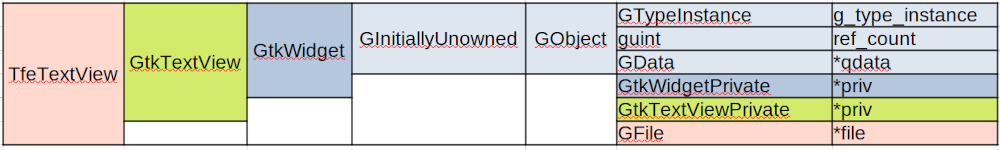
\includegraphics[width=14.39cm,height=2.16cm]{../image/TfeTextView.png}
\caption{The structure of the instance TfeTextView}
\end{figure}

\hypertarget{initialization-of-a-tfetextview-instance}{%
\subsection{Initialization of a TfeTextView
instance}\label{initialization-of-a-tfetextview-instance}}

The function \passthrough{\lstinline!tfe\_text\_view\_new!} creates a
new TfeTextView instance.

\begin{lstlisting}[language=C, numbers=left]
GtkWidget *
tfe_text_view_new (void) {
  return GTK_WIDGET (g_object_new (TFE_TYPE_TEXT_VIEW, NULL));
}
\end{lstlisting}

When this function is involed, a TfeTextView instance is created and
initialized. The initialization process is as follows.

\begin{enumerate}
\def\labelenumi{\arabic{enumi}.}
\tightlist
\item
  Initializes GObject (GInitiallyUnowned) part in TfeTextView instance.
\item
  Initializes GtkWidget part in TfeTextView instance.
\item
  Initializes GtkTextView part in TfeTextView instance.
\item
  Initializes TfeTextView part in TfeTextView instance.
\end{enumerate}

The step one through three is done by
\passthrough{\lstinline!g\_object\_init!},
\passthrough{\lstinline!gtk\_widget\_init!} and
\passthrough{\lstinline!gtk\_text\_view\_init!}. They are called by the
system automatically and you don't need to care about them. Step four is
done by the function \passthrough{\lstinline!tfe\_text\_view\_init!} in
\passthrough{\lstinline!tfetextview.c!}.

\begin{lstlisting}[language=C, numbers=left]
static void
tfe_text_view_init (TfeTextView *tv) {
  tv->file = NULL;
}
\end{lstlisting}

This function just initializes \passthrough{\lstinline!tv->file!} to be
\passthrough{\lstinline!NULL!}.

\hypertarget{functions-and-classes}{%
\subsection{Functions and Classes}\label{functions-and-classes}}

In Gtk, all objects derived from GObject have class and instance (except
abstract object). An instance is memory of C structure, which is
described in the previous two subsections. Each object can have more
than one instance. Those instances have the same structure. An instance
just keeps status of the instance. Therefore, it is insufficient to
define its behavior. We need at least two things. One is functions and
the other is class.

You've already seen many functions. For example,
\passthrough{\lstinline!tfe\_text\_view\_new!} is a function to create a
TfeTextView instance. These functions are similar to public object
methods in object oriented languages such as Java or Ruby. Functions are
public, which means that they are expected to be used by other objects.

Class comprises mainly pointers to functions. Those functions are used
by the object itself or its descendant objects. For example, GObject
class is declared in \passthrough{\lstinline!gobject.h!} in GLib source
files.

\begin{lstlisting}[language=C, numbers=left]
typedef struct _GObjectClass             GObjectClass;
typedef struct _GObjectClass             GInitiallyUnownedClass;

struct  _GObjectClass
{
  GTypeClass   g_type_class;
  /*< private >*/
  GSList      *construct_properties;
  /*< public >*/
  /* seldom overridden */
  GObject*   (*constructor)     (GType                  type,
                                 guint                  n_construct_properties,
                                 GObjectConstructParam *construct_properties);
  /* overridable methods */
  void       (*set_property)    (GObject        *object,
                                 guint           property_id,
                                 const GValue   *value,
                                 GParamSpec     *pspec);
  void       (*get_property)    (GObject        *object,
                                 guint           property_id,
                                 GValue         *value,
                                 GParamSpec     *pspec);
  void       (*dispose)         (GObject        *object);
  void       (*finalize)        (GObject        *object);
  /* seldom overridden */
  void       (*dispatch_properties_changed) (GObject      *object,
                                             guint         n_pspecs,
                                             GParamSpec  **pspecs);
  /* signals */
  void      (*notify)           (GObject    *object,
                                 GParamSpec *pspec);
  /* called when done constructing */
  void      (*constructed)      (GObject    *object);
  /*< private >*/
  gsize  flags;
  /* padding */
  gpointer pdummy[6];
};
\end{lstlisting}

I'd like to explain some of the members. There's a pointer to the
function \passthrough{\lstinline!dispose!} in line 23.

\begin{lstlisting}[language=C]
void (*dispose) (GObject *object);
\end{lstlisting}

The declaration is a bit complicated. The asterisk before the identifier
\passthrough{\lstinline!dispose!} means pointer. So, the pointer
\passthrough{\lstinline!dispose!} points to a function which has one
parameter, which points a GObject structure, and returns no value. In
the same way, line 24 says \passthrough{\lstinline!finalize!} is a
pointer to the function which has one parameter, which points a GObject
structure, and returns no value.

\begin{lstlisting}[language=C]
void (*finalize) (GObject *object);
\end{lstlisting}

Look at the declaration of \passthrough{\lstinline!\_GObjectClass!} so
that you would find that most of the members are pointers to functions.

\begin{itemize}
\tightlist
\item
  11: A function pointed by \passthrough{\lstinline!constructor!} is
  called when the instance is generated. It completes the initialization
  of the instance.
\item
  23: A function pointed by \passthrough{\lstinline!dispose!} is called
  when the instance destructs itself. Destruction process is divided
  into two phases. The first one is called disposing. In this phase, the
  instance releases all the references to other instances. The second
  phase is finalizing.
\item
  24: A function pointed by \passthrough{\lstinline!finalize!} finishes
  the destruction process.
\item
  The other pointers point to functions which are called while the
  instance lives.
\end{itemize}

These functions are called class methods. The methods are open to its
descendants. But not open to the objects which are not the descendants.

\hypertarget{tfetextview-class}{%
\subsection{TfeTextView class}\label{tfetextview-class}}

TfeTextView class is a structure and it includes all its ancestors'
class in it.

\begin{lstlisting}[language=C]
typedef _TfeTextView TfeTextView;
struct _TfeTextView {
  GtkTextView parent;
  GFile *file;
};
\end{lstlisting}

TfeTextView structure has GtkTextView type as the first member. In the
same way, GtkTextView has its parent type (GtkWidget) as the first
member. GtkWidget has its parent type (GtkInitiallyUnowned) as the first
member. The structure of GtkInitiallyUnowned is the same as GObject.
Therefore, TFeTextView includes GObject, GtkWidget and GtkTextView in
itself.

\begin{lstlisting}
GObject -- GInitiallyUnowned -- GtkWidget -- GtkTextView -- TfeTextView
\end{lstlisting}

The following is extracts from the source files (not exactly the same).

\begin{lstlisting}[language=C, numbers=left]
struct _GtkWidgetClass
{
  GInitiallyUnownedClass parent_class;

  /*< public >*/

  /* basics */
  void (* show)                (GtkWidget        *widget);
  void (* hide)                (GtkWidget        *widget);
  void (* map)                 (GtkWidget        *widget);
  void (* unmap)               (GtkWidget        *widget);
  void (* realize)             (GtkWidget        *widget);
  void (* unrealize)           (GtkWidget        *widget);
  void (* root)                (GtkWidget        *widget);
  void (* unroot)              (GtkWidget        *widget);
  void (* size_allocate)       (GtkWidget           *widget,
                                int                  width,
                                int                  height,
                                int                  baseline);
  void (* state_flags_changed) (GtkWidget        *widget,
                                GtkStateFlags     previous_state_flags);
  void (* direction_changed)   (GtkWidget        *widget,
                                GtkTextDirection  previous_direction);

  /* size requests */
  GtkSizeRequestMode (* get_request_mode)               (GtkWidget      *widget);
  void              (* measure) (GtkWidget      *widget,
                                 GtkOrientation  orientation,
                                 int             for_size,
                                 int            *minimum,
                                 int            *natural,
                                 int            *minimum_baseline,
                                 int            *natural_baseline);

  /* Mnemonics */
  gboolean (* mnemonic_activate)        (GtkWidget           *widget,
                                         gboolean             group_cycling);

  /* explicit focus */
  gboolean (* grab_focus)               (GtkWidget           *widget);
  gboolean (* focus)                    (GtkWidget           *widget,
                                         GtkDirectionType     direction);
  void     (* set_focus_child)          (GtkWidget           *widget,
                                         GtkWidget           *child);

  /* keyboard navigation */
  void     (* move_focus)               (GtkWidget           *widget,
                                         GtkDirectionType     direction);
  gboolean (* keynav_failed)            (GtkWidget           *widget,
                                         GtkDirectionType     direction);

  gboolean     (* query_tooltip)      (GtkWidget  *widget,
                                       int         x,
                                       int         y,
                                       gboolean    keyboard_tooltip,
                                       GtkTooltip *tooltip);

  void         (* compute_expand)     (GtkWidget  *widget,
                                       gboolean   *hexpand_p,
                                       gboolean   *vexpand_p);

  void         (* css_changed)                 (GtkWidget            *widget,
                                                GtkCssStyleChange    *change);

  void         (* system_setting_changed)      (GtkWidget            *widget,
                                                GtkSystemSetting      settings);

  void         (* snapshot)                    (GtkWidget            *widget,
                                                GtkSnapshot          *snapshot);

  gboolean     (* contains)                    (GtkWidget *widget,
                                                double     x,
                                                double     y);

  /*< private >*/

  GtkWidgetClassPrivate *priv;

  gpointer padding[8];
};

struct _GtkTextViewClass
{
  GtkWidgetClass parent_class;

  /*< public >*/

  void (* move_cursor)           (GtkTextView      *text_view,
                                  GtkMovementStep   step,
                                  int               count,
                                  gboolean          extend_selection);
  void (* set_anchor)            (GtkTextView      *text_view);
  void (* insert_at_cursor)      (GtkTextView      *text_view,
                                  const char       *str);
  void (* delete_from_cursor)    (GtkTextView      *text_view,
                                  GtkDeleteType     type,
                                  int               count);
  void (* backspace)             (GtkTextView      *text_view);
  void (* cut_clipboard)         (GtkTextView      *text_view);
  void (* copy_clipboard)        (GtkTextView      *text_view);
  void (* paste_clipboard)       (GtkTextView      *text_view);
  void (* toggle_overwrite)      (GtkTextView      *text_view);
  GtkTextBuffer * (* create_buffer) (GtkTextView   *text_view);
  void (* snapshot_layer)        (GtkTextView      *text_view,
                                  GtkTextViewLayer  layer,
                                  GtkSnapshot      *snapshot);
  gboolean (* extend_selection)  (GtkTextView            *text_view,
                                  GtkTextExtendSelection  granularity,
                                  const GtkTextIter      *location,
                                  GtkTextIter            *start,
                                  GtkTextIter            *end);
  void (* insert_emoji)          (GtkTextView      *text_view);

  /*< private >*/

  gpointer padding[8];
};

/* The following definition is generated by the macro G_DECLARE_FINAL_TYPE */
typedef struct {
  GtkTextView parent_class;
} TfeTextViewClass;
\end{lstlisting}

\begin{itemize}
\tightlist
\item
  120-122: This three lines are generated by the macro
  \passthrough{\lstinline!G\_DECLARE\_FINAL\_TYPE!}. So, they are not
  written in either \passthrough{\lstinline!tfe\_text\_view.h!} or
  \passthrough{\lstinline!tfe\_text\_view.c!}.
\item
  3, 84, 121: Each derived class puts its parent class at the first
  member of its structure. It is the same as instance structures.
\item
  Class members in ancestors are open to the descendant class. So, they
  can be changed in
  \passthrough{\lstinline!tfe\_text\_view\_class\_init!} function. For
  example, the \passthrough{\lstinline!dispose!} pointer in GObjectClass
  will be overridden later in
  \passthrough{\lstinline!tfe\_text\_view\_class\_init!}. (Override is
  an object oriented programming terminology. Override is rewriting
  ancestors' class methods in the descendant class.)
\item
  Some class methods are often overridden.
  \passthrough{\lstinline!set\_property!},
  \passthrough{\lstinline!get\_property!},
  \passthrough{\lstinline!dispose!}, \passthrough{\lstinline!finalize!}
  and \passthrough{\lstinline!constructed!} are such methods.
\end{itemize}

TfeTextViewClass includes its ancestors' class in it. It is illustrated
in the following diagram.

\begin{figure}
\centering
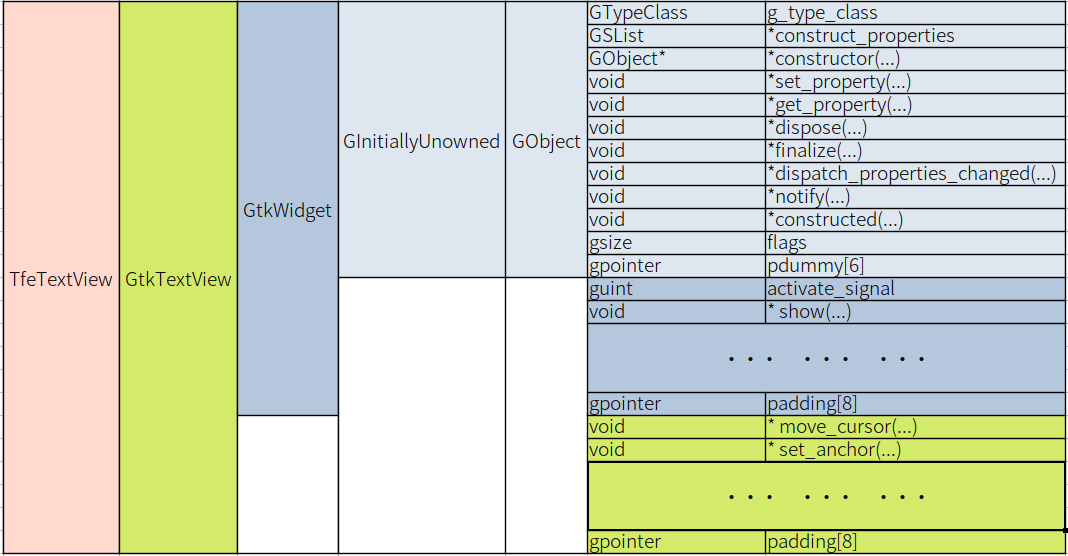
\includegraphics[width=16.02cm,height=8.34cm]{../image/TfeTextViewClass.png}
\caption{The structure of TfeTextView Class}
\end{figure}

\hypertarget{destruction-of-tfetextview}{%
\subsection{Destruction of
TfeTextView}\label{destruction-of-tfetextview}}

Every Object derived from GObject has a reference count. If an object A
refers to an object B, then A keeps a pointer to B in A and at the same
time increases the reference count of B by one with the function
\passthrough{\lstinline!g\_object\_ref (B)!}. If A doesn't need B any
longer, then A discards the pointer to B (usually it is done by
assigning NULL to the pointer) and decreases the reference count of B by
one with the function \passthrough{\lstinline!g\_object\_unref (B)!}.

If two objects A and B refer to C, then the reference count of C is two.
If A no longer needs C, A discards the pointer to C and decreases the
reference count in C by one. Now the reference count of C is one. In the
same way, if B no longer needs C, B discards the pointer to C and
decreases the reference count in C by one. At this moment, no object
refers to C and the reference count of C is zero. This means C is no
longer useful. Then C destructs itself and finally the memories
allocated to C is freed.

\begin{figure}
\centering
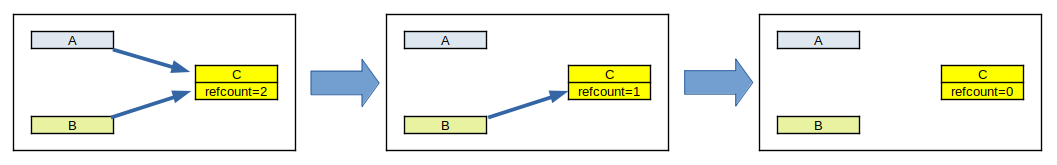
\includegraphics[width=15.855cm,height=2.475cm]{../image/refcount.png}
\caption{Reference count of B}
\end{figure}

The idea above is based on an assumption that an object referred by
nothing has reference count of zero. When the reference count drops to
zero, the object starts its destruction process. The destruction process
is split into two phases: disposing and finalizing. In the disposing
process, the object invokes the function pointed by
\passthrough{\lstinline!dispose!} in its class to release all references
to other objects. In the finalizing process, it invokes the function
pointed by \passthrough{\lstinline!finalize!} in its class to complete
the destruction process. These functions are also called handlers or
methods. For example, dispose handler or dispose method.

In the destruction process of TfeTextView, the reference count of
widgets related to TfeTextView is automatically decreased. But GFile
pointed by \passthrough{\lstinline!tv->file!} needs to decrease its
reference count by one. You must write the code in the dispose handler
\passthrough{\lstinline!tfe\_text\_view\_dispose!}.

\begin{lstlisting}[language=C, numbers=left]
static void
tfe_text_view_dispose (GObject *gobject) {
  TfeTextView *tv = TFE_TEXT_VIEW (gobject);

  if (G_IS_FILE (tv->file))
    g_clear_object (&tv->file);

  G_OBJECT_CLASS (tfe_text_view_parent_class)->dispose (gobject);
}
\end{lstlisting}

\begin{itemize}
\tightlist
\item
  5,6: If \passthrough{\lstinline!tv->file!} points a GFile, decrease
  its reference count. \passthrough{\lstinline!g\_clear\_object!}
  decreases the reference count and assigns NULL to
  \passthrough{\lstinline!tv->file!}. In dispose handlers, we usually
  use \passthrough{\lstinline!g\_clear\_object!} rather than
  \passthrough{\lstinline!g\_object\_unref!}.
\item
  8: invokes parent's dispose handler. (This will be explained later.)
\end{itemize}

In the disposing process, the object uses the pointer in its class to
call the handler. Therefore,
\passthrough{\lstinline!tfe\_text\_view\_dispose!} needs to be
registered in the class when the TfeTextView class is initialized. The
function \passthrough{\lstinline!tfe\_text\_view\_class\_init!} is the
class initialization function and it is declared in the replacement
produced by \passthrough{\lstinline!G\_DEFINE\_TYPE!} macro.

\begin{lstlisting}[language=C]
static void
tfe_text_view_class_init (TfeTextViewClass *class) {
  GObjectClass *object_class = G_OBJECT_CLASS (class);

  object_class->dispose = tfe_text_view_dispose;

}
\end{lstlisting}

Each ancestors' class has been created before TfeTextViewClass is
created. Therefore, there are four classes and each class has a pointer
to each dispose handler. Look at the following diagram. There are four
classes -- GObjectClass (GInitiallyUnownedClass), GtkWidgetClass,
GtkTextViewClass and TfeTextViewClass. Each class has its own dispose
handler -- \passthrough{\lstinline!dh1!}, \passthrough{\lstinline!dh2!},
\passthrough{\lstinline!dh3!} and
\passthrough{\lstinline!tfe\_text\_view\_dispose!}.

\begin{figure}
\centering
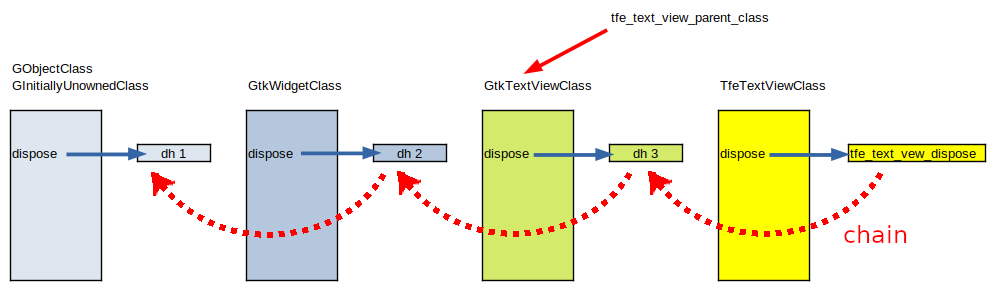
\includegraphics[width=14.925cm,height=4.455cm]{../image/dispose_handler.png}
\caption{dispose handlers}
\end{figure}

Now, look at the \passthrough{\lstinline!tfe\_text\_view\_dispose!}
program above. It first releases the reference to GFile object pointed
by \passthrough{\lstinline!tv->file!}. Then it invokes its parent's
dispose handler in line 8.

\begin{lstlisting}[language=C]
G_OBJECT_CLASS (tfe_text_view_parent_class)->dispose (gobject);
\end{lstlisting}

\passthrough{\lstinline!tfe\_text\_view\_parent\_class!},which is made
by \passthrough{\lstinline!G\_DEFINE\_TYPE!} macro, is a pointer that
points the parent object class. Therefore,
\passthrough{\lstinline!G\_OBJECT\_CLASS (tfe\_text\_view\_parent\_class)->dispose!}
points the handler \passthrough{\lstinline!dh3!} in the diagram above.
And \passthrough{\lstinline!gobject!} is a pointer to TfeTextView
instance which is casted as a GObject instance.
\passthrough{\lstinline!dh3!} releases all the references to objects in
the GtkTextView part (it is actually the private area pointed by
\passthrough{\lstinline!prev!}) in TfeTextView instance. After that,
\passthrough{\lstinline!dh3!} calls \passthrough{\lstinline!dh2!}, and
\passthrough{\lstinline!dh2!} calls \passthrough{\lstinline!dh1!}.
Finally all the references are released.

  \hypertarget{signals}{%
\section{Signals}\label{signals}}

\hypertarget{signals-1}{%
\subsection{Signals}\label{signals-1}}

In Gtk programming, each object is encapsulated. And it is not
recommended to use global variables because they tend to make the
program complicated. So, we need something to communicate between
objects. There are two ways to do so.

\begin{itemize}
\tightlist
\item
  Functions. For example,
  \passthrough{\lstinline!tb = gtk\_text\_view\_get\_buffer (tv)!}. The
  caller requests \passthrough{\lstinline!tv!} to give
  \passthrough{\lstinline!tb!}, which is a GtkTextBuffer instance
  connected to \passthrough{\lstinline!tv!} to the caller.
\item
  Signals. For example, \passthrough{\lstinline!activate!} signal on
  GApplication object. When the application is activated, the signal is
  emitted. Then the handler, which has been connected to the signal, is
  invoked.
\end{itemize}

The caller of the function or the handler connected to the signal is
usually out of the object. One of the difference between these two is
that the object is active or passive. In functions the object passively
responds to the caller. In signals the object actively sends a signal to
the handler.

GObject signals are registered, connected and emitted.

\begin{enumerate}
\def\labelenumi{\arabic{enumi}.}
\tightlist
\item
  Signals are registered with the object type on which they are emitted.
  The registration is done usually when the object class is initialized.
\item
  Signals are connected to handlers by
  \passthrough{\lstinline!g\_connect\_signal!} or its family functions.
  The connection is usually done out of the object.
\item
  When Signals are emitted, the connected handlers are invoked. Signal
  is emitted on the instance of the object.
\end{enumerate}

\hypertarget{signal-registration}{%
\subsection{Signal registration}\label{signal-registration}}

In TfeTextView, two signals are registered.

\begin{itemize}
\tightlist
\item
  ``change-file'' signal. This signal is emitted when
  \passthrough{\lstinline!tv->file!} is changed.
\item
  ``open-response'' signal.
  \passthrough{\lstinline!tfe\_text\_view\_open!} function is not able
  to return the status because it uses GtkFileChooserDialog. This signal
  is emitted instead of the return value of the function.
\end{itemize}

A static variable or array is used to store the signal ID. A static
array is used to register two or more signals.

\begin{lstlisting}[language=C]
enum {
  CHANGE_FILE,
  OPEN_RESPONSE,
  NUMBER_OF_SIGNALS
};

static guint tfe_text_view_signals[NUMBER_OF_SIGNALS];
\end{lstlisting}

Signals are registered in the class initialization function.

\begin{lstlisting}[language=C, numbers=left]
static void
tfe_text_view_class_init (TfeTextViewClass *class) {
  GObjectClass *object_class = G_OBJECT_CLASS (class);

  object_class->dispose = tfe_text_view_dispose;
  tfe_text_view_signals[CHANGE_FILE] = g_signal_new ("change-file",
                                 G_TYPE_FROM_CLASS (class),
                                 G_SIGNAL_RUN_LAST | G_SIGNAL_NO_RECURSE | G_SIGNAL_NO_HOOKS,
                                 0 /* class offset */,
                                 NULL /* accumulator */,
                                 NULL /* accumulator data */,
                                 NULL /* C marshaller */,
                                 G_TYPE_NONE /* return_type */,
                                 0     /* n_params */
                                 );
  tfe_text_view_signals[OPEN_RESPONSE] = g_signal_new ("open-response",
                                 G_TYPE_FROM_CLASS (class),
                                 G_SIGNAL_RUN_LAST | G_SIGNAL_NO_RECURSE | G_SIGNAL_NO_HOOKS,
                                 0 /* class offset */,
                                 NULL /* accumulator */,
                                 NULL /* accumulator data */,
                                 NULL /* C marshaller */,
                                 G_TYPE_NONE /* return_type */,
                                 1     /* n_params */,
                                 G_TYPE_INT
                                 );
}
\end{lstlisting}

\begin{itemize}
\tightlist
\item
  6-15: Registers ``change-file'' signal.
  \passthrough{\lstinline!g\_signal\_new!} function is used. The signal
  ``change-file'' has no default handler (object method handler). You
  usually don't need to set a default handler. If you need it, use
  \passthrough{\lstinline!g\_signal\_new\_class\_handler!} function. See
  \href{https://docs.gtk.org/gobject/func.signal_new_class_handler.html}{GObject
  API Reference, g\_signal\_new\_class\_handler} for further
  information.
\item
  The return value of \passthrough{\lstinline!g\_signal\_new!} is the
  signal id. The type of signal id is guint, which is the same as
  unsigned int. It is used in the function
  \passthrough{\lstinline!g\_signal\_emit!}.
\item
  16-26: Registers ``open-response'' signal. This signal has a
  parameter.
\item
  24: Number of the parameters. ``open-response'' signal has one
  parameter.
\item
  25: The type of the parameter. \passthrough{\lstinline!G\_TYPE\_INT!}
  is a type of integer. Such fundamental types are described in
  \href{https://developer-old.gnome.org/gobject/stable/gobject-Type-Information.html}{GObject
  reference manual}.
\end{itemize}

The handlers are declared as follows.

\begin{lstlisting}[language=C]
/* "change-file" signal handler */
void
user_function (TfeTextView *tv,
               gpointer user_data)

/* "open-response" signal handler */
void
user_function (TfeTextView *tv,
               TfeTextViewOpenResponseType response-id,
               gpointer user_data)
\end{lstlisting}

\begin{itemize}
\tightlist
\item
  Because ``change-file'' signal doesn't have parameter, the handler's
  parameters are a TfeTextView instance and user data.
\item
  Because ``open-response'' signal has one parameter, the handler's
  parameters are a TfeTextView instance, the signal's parameter and user
  data.
\item
  \passthrough{\lstinline!tv!} is the object instance on which the
  signal is emitted.
\item
  \passthrough{\lstinline!user\_data!} comes from the fourth argument of
  \passthrough{\lstinline!g\_signal\_connect!}.
\item
  \passthrough{\lstinline!parameter!} comes from the fourth argument of
  \passthrough{\lstinline!g\_signal\_emit!}.
\end{itemize}

The values of the parameter is defined in
\passthrough{\lstinline!tfetextview.h!} because they are public.

\begin{lstlisting}[language=C]
/* "open-response" signal response */
enum
{
  TFE_OPEN_RESPONSE_SUCCESS,
  TFE_OPEN_RESPONSE_CANCEL,
  TFE_OPEN_RESPONSE_ERROR
};
\end{lstlisting}

\begin{itemize}
\tightlist
\item
  The parameter is set to
  \passthrough{\lstinline!TFE\_OPEN\_RESPONSE\_SUCCESS!} when
  \passthrough{\lstinline!tfe\_text\_view\_open!} has successfully
  opened a file and read it.
\item
  The parameter is set to
  \passthrough{\lstinline!TFE\_OPEN\_RESPONSE\_CANCEL!} when the user
  has canceled.
\item
  The parameter is set to
  \passthrough{\lstinline!TFE\_OPEN\_RESPONSE\_ERROR!} when an error has
  occurred.
\end{itemize}

\hypertarget{signal-connection}{%
\subsection{Signal connection}\label{signal-connection}}

A signal and a handler are connected by the function
\passthrough{\lstinline!g\_signal\_connect!}. There are some similar
functions like \passthrough{\lstinline!g\_signal\_connect\_after!},
\passthrough{\lstinline!g\_signal\_connect\_swapped!} and so on.
However, \passthrough{\lstinline!g\_signal\_connect!} is the most
common. The signals ``change-file'' is connected to a callback function
out of the TfeTextView object. In the same way, the signals
``open-response'' is connected to a callback function out of the
TfeTextView object. Those callback functions are defined by users.

In the program \passthrough{\lstinline!tfe!}, callback functions are
defined in \passthrough{\lstinline!tfenotebook.c!}. And their names are
\passthrough{\lstinline!file\_changed!} and
\passthrough{\lstinline!open\_response!}. They will be explained later.

\begin{lstlisting}[language=C]
g_signal_connect (GTK_TEXT_VIEW (tv), "change-file", G_CALLBACK (file_changed), nb);

g_signal_connect (TFE_TEXT_VIEW (tv), "open-response", G_CALLBACK (open_response), nb);
\end{lstlisting}

\hypertarget{signal-emission}{%
\subsection{Signal emission}\label{signal-emission}}

Signals are emitted on an instance. The type of the instance is the
second argument of \passthrough{\lstinline!g\_signal\_new!}. The
relationship between the signal and object type is determined when the
signal is registered.

A function \passthrough{\lstinline!g\_signal\_emit!} is used to emit the
signal. The following lines are extracted from
\passthrough{\lstinline!tfetextview.c!}. Each line comes from a
different line.

\begin{lstlisting}[language=C]
g_signal_emit (tv, tfe_text_view_signals[CHANGE_FILE], 0);
g_signal_emit (tv, tfe_text_view_signals[OPEN_RESPONSE], 0, TFE_OPEN_RESPONSE_SUCCESS);
g_signal_emit (tv, tfe_text_view_signals[OPEN_RESPONSE], 0, TFE_OPEN_RESPONSE_CANCEL);
g_signal_emit (tv, tfe_text_view_signals[OPEN_RESPONSE], 0, TFE_OPEN_RESPONSE_ERROR);
\end{lstlisting}

\begin{itemize}
\tightlist
\item
  The first argument is the instance on which the signal is emitted.
\item
  The second argument is the signal id.
\item
  The third argument is the detail of the signal. ``change-file'' signal
  and ``open-response'' signal doesn't have details and the argument is
  zero when no details.
\item
  ``change-file'' signal doesn't have parameter, so there's no fourth
  parameter.
\item
  ``open-response'' signal has one parameter. The fourth parameter is
  the parameter.
\end{itemize}

  \hypertarget{functions-in-tfetextview}{%
\section{Functions in TfeTextView}\label{functions-in-tfetextview}}

In this section I will explain functions in TfeTextView object.

\hypertarget{tfe.h-and-tfetextview.h}{%
\subsection{tfe.h and tfetextview.h}\label{tfe.h-and-tfetextview.h}}

\passthrough{\lstinline!tfe.h!} is a top header file and it includes
\passthrough{\lstinline!gtk.h!} and all the header files. C source files
\passthrough{\lstinline!tfeapplication.c!} and
\passthrough{\lstinline!tfenotebook.c!} include
\passthrough{\lstinline!tfe.h!} at the beginning.

\begin{lstlisting}[language=C, numbers=left]
#include <gtk/gtk.h>

#include "../tfetextview/tfetextview.h"
#include "tfenotebook.h"
\end{lstlisting}

\passthrough{\lstinline!../tfetextview/tfetextview.h!} is a header file
which describes the public functions in
\passthrough{\lstinline!tfetextview.c!}.

\begin{lstlisting}[language=C, numbers=left]
#ifndef __TFE_TEXT_VIEW_H__
#define __TFE_TEXT_VIEW_H__

#include <gtk/gtk.h>

#define TFE_TYPE_TEXT_VIEW tfe_text_view_get_type ()
G_DECLARE_FINAL_TYPE (TfeTextView, tfe_text_view, TFE, TEXT_VIEW, GtkTextView)

/* "open-response" signal response */
enum TfeTextViewOpenResponseType
{
  TFE_OPEN_RESPONSE_SUCCESS,
  TFE_OPEN_RESPONSE_CANCEL,
  TFE_OPEN_RESPONSE_ERROR
};

GFile *
tfe_text_view_get_file (TfeTextView *tv);

void
tfe_text_view_open (TfeTextView *tv, GtkWindow *win);

void
tfe_text_view_save (TfeTextView *tv);

void
tfe_text_view_saveas (TfeTextView *tv);

GtkWidget *
tfe_text_view_new_with_file (GFile *file);

GtkWidget *
tfe_text_view_new (void);

#endif /* __TFE_TEXT_VIEW_H__ */
\end{lstlisting}

\begin{itemize}
\tightlist
\item
  1,2,35: Thanks to these three lines, the following lines are included
  only once.
\item
  4: Includes gtk4 header files. The header file
  \passthrough{\lstinline!gtk4!} also has the same mechanism to avoid
  including it multiple times.
\item
  6-7: These two lines define TfeTextView type, its class structure and
  some useful macros.
\item
  9-15: A definition of the value of the parameter of ``open-response''
  signal.
\item
  17-33: Declarations of public functions on TfeTextView.
\end{itemize}

\hypertarget{functions-to-create-tfetextview-instances}{%
\subsection{Functions to create TfeTextView
instances}\label{functions-to-create-tfetextview-instances}}

A TfeTextView instance is created with
\passthrough{\lstinline!tfe\_text\_view\_new!} or
\passthrough{\lstinline!tfe\_text\_view\_new\_with\_file!}.

\begin{lstlisting}[language=C]
GtkWidget *tfe_text_view_new (void);
\end{lstlisting}

\passthrough{\lstinline!tfe\_text\_view\_new!} just creates a new
TfeTextView instance and returns the pointer to the new instance.

\begin{lstlisting}[language=C]
GtkWidget *tfe_text_view_new_with_file (GFile *file);
\end{lstlisting}

\passthrough{\lstinline!tfe\_text\_view\_new\_with\_file!} is given a
Gfile object as an argument and it loads the file into the GtkTextBuffer
instance, then returns the pointer to the new instance. If an error
occurs during the creation process, NULL is returned.

Each function is defined as follows.

\begin{lstlisting}[language=C, numbers=left]
GtkWidget *
tfe_text_view_new_with_file (GFile *file) {
  g_return_val_if_fail (G_IS_FILE (file), NULL);

  GtkWidget *tv;
  GtkTextBuffer *tb;
  char *contents;
  gsize length;

  if (! g_file_load_contents (file, NULL, &contents, &length, NULL, NULL)) /* read error */
    return NULL;

  if ((tv = tfe_text_view_new()) != NULL) {
    tb = gtk_text_view_get_buffer (GTK_TEXT_VIEW (tv));
    gtk_text_buffer_set_text (tb, contents, length);
    TFE_TEXT_VIEW (tv)->file = g_file_dup (file);
    gtk_text_buffer_set_modified (tb, FALSE);
  }
  g_free (contents);
  return tv;
}

GtkWidget *
tfe_text_view_new (void) {
  return GTK_WIDGET (g_object_new (TFE_TYPE_TEXT_VIEW, NULL));
}
\end{lstlisting}

\begin{itemize}
\tightlist
\item
  23-25: \passthrough{\lstinline!tfe\_text\_view\_new!} function. Just
  returns the value from the function
  \passthrough{\lstinline!g\_object\_new!} but casts it to the pointer
  to GtkWidget. Initialization is done in
  \passthrough{\lstinline!tfe\_text\_view\_init!} which is called in the
  process of \passthrough{\lstinline!g\_object\_new!} function.
\item
  1-21: \passthrough{\lstinline!tfe\_text\_view\_new\_with\_file!}
  function.
\item
  3: \passthrough{\lstinline!g\_return\_val\_if\_fail!} is described in
  \href{https://docs.gtk.org/glib/func.return_val_if_fail.html}{GLib API
  Reference, g\_return\_val\_if\_fail}. And also
  \href{https://docs.gtk.org/glib/logging.html}{GLib API Reference,
  Message Logging}. It tests whether the argument
  \passthrough{\lstinline!file!} is a pointer to GFile. If it's true,
  then the program goes on to the next line. If it's false, then it
  returns NULL (the second argument) immediately. And at the same time
  it logs out the error message (usually the log is outputted to stderr
  or stdout). This function is used to check the programmer's error. If
  an error occurs, the solution is usually to change the (caller)
  program and fix the bug. You need to distinguish programmer's errors
  and runtime errors. You shouldn't use this function to find runtime
  errors.
\item
  10-11: If an error occurs when reading the file, then the function
  returns NULL.
\item
  13: Calls the function \passthrough{\lstinline!tfe\_text\_view\_new!}.
  The function creates TfeTextView instance and returns the pointer to
  the instance. If an error happens in
  \passthrough{\lstinline!tfe\_text\_view\_new!}, it returns NULL.
\item
  14: Gets the pointer to GtkTextBuffer corresponds to
  \passthrough{\lstinline!tv!}. The pointer is assigned to
  \passthrough{\lstinline!tb!}
\item
  15: Assigns the contents read from the file to GtkTextBuffer pointed
  by \passthrough{\lstinline!tb!}.
\item
  16: Duplicates \passthrough{\lstinline!file!} and sets
  \passthrough{\lstinline!tv->file!} to point it.
\item
  17: The function
  \passthrough{\lstinline!gtk\_text\_buffer\_set\_modified (tb, FALSE)!}
  sets the modification flag of \passthrough{\lstinline!tb!} to FALSE.
  The modification flag indicates that the contents of the buffer is
  modified. It is used when the contents are saved. If the modification
  flag is FALSE, it doesn't need to save the contents.
\item
  19: Frees the memories pointed by \passthrough{\lstinline!contents!}.
\item
  20: Returns \passthrough{\lstinline!tv!}, which is a pointer to the
  newly created TfeTextView instance. If an error happens, NULL is
  returned.
\end{itemize}

\hypertarget{save-and-saveas-functions}{%
\subsection{Save and saveas functions}\label{save-and-saveas-functions}}

Save and saveas functions write the contents in the GtkTextBuffer to a
file.

\begin{lstlisting}[language=C]
void tfe_text_view_save (TfeTextView *tv)
\end{lstlisting}

The function \passthrough{\lstinline!tfe\_text\_view\_save!} writes the
contents in the GtkTextBuffer to a file specified by
\passthrough{\lstinline!tv->file!}. If
\passthrough{\lstinline!tv->file!} is NULL, then it shows
GtkFileChooserDialog and prompts the user to choose a file to save. Then
it saves the contents to the file and sets
\passthrough{\lstinline!tv->file!} to point the GFile instance for the
file.

\begin{lstlisting}[language=C]
void tfe_text_view_saveas (TfeTextView *tv)
\end{lstlisting}

The function \passthrough{\lstinline!saveas!} uses GtkFileChooserDialog
and prompts the user to select a existed file or specify a new file to
save. Then, the function changes \passthrough{\lstinline!tv->file!} and
save the contents to the specified file. If an error occurs, it is shown
to the user through the message dialog. The error is managed only in the
TfeTextView and no information is notified to the caller.

\begin{lstlisting}[language=C, numbers=left]
static gboolean
save_file (GFile *file, GtkTextBuffer *tb, GtkWindow *win) {
  GtkTextIter start_iter;
  GtkTextIter end_iter;
  gchar *contents;
  gboolean stat;
  GtkWidget *message_dialog;
  GError *err = NULL;

  gtk_text_buffer_get_bounds (tb, &start_iter, &end_iter);
  contents = gtk_text_buffer_get_text (tb, &start_iter, &end_iter, FALSE);
  if (g_file_replace_contents (file, contents, strlen (contents), NULL, TRUE, G_FILE_CREATE_NONE, NULL, NULL, &err)) {
    gtk_text_buffer_set_modified (tb, FALSE);
    stat = TRUE;
  } else {
    message_dialog = gtk_message_dialog_new (win, GTK_DIALOG_MODAL,
                                             GTK_MESSAGE_ERROR, GTK_BUTTONS_CLOSE,
                                            "%s.\n", err->message);
    g_signal_connect (message_dialog, "response", G_CALLBACK (gtk_window_destroy), NULL);
    gtk_widget_show (message_dialog);
    g_error_free (err);
    stat = FALSE;
  }
  g_free (contents);
  return stat;
}

static void
saveas_dialog_response (GtkWidget *dialog, gint response, TfeTextView *tv) {
  GtkTextBuffer *tb = gtk_text_view_get_buffer (GTK_TEXT_VIEW (tv));
  GFile *file;
  GtkWidget *win = gtk_widget_get_ancestor (GTK_WIDGET (tv), GTK_TYPE_WINDOW);

  if (response == GTK_RESPONSE_ACCEPT) {
    file = gtk_file_chooser_get_file (GTK_FILE_CHOOSER (dialog));
    if (! G_IS_FILE (file))
      g_warning ("TfeTextView: gtk_file_chooser_get_file returns non GFile.\n");
    else if (save_file(file, tb, GTK_WINDOW (win))) {
      if (G_IS_FILE (tv->file))
        g_object_unref (tv->file);
      tv->file = file;
      g_signal_emit (tv, tfe_text_view_signals[CHANGE_FILE], 0);
    } else
      g_object_unref (file);
  }
  gtk_window_destroy (GTK_WINDOW (dialog));
}

void
tfe_text_view_save (TfeTextView *tv) {
  g_return_if_fail (TFE_IS_TEXT_VIEW (tv));

  GtkTextBuffer *tb = gtk_text_view_get_buffer (GTK_TEXT_VIEW (tv));
  GtkWidget *win = gtk_widget_get_ancestor (GTK_WIDGET (tv), GTK_TYPE_WINDOW);

  if (! gtk_text_buffer_get_modified (tb))
    return; /* no need to save it */
  else if (tv->file == NULL)
    tfe_text_view_saveas (tv);
  else if (! G_IS_FILE (tv->file))
    g_error ("TfeTextView: The pointer tv->file isn't NULL nor GFile.\n");
  else
    save_file (tv->file, tb, GTK_WINDOW (win));
}

void
tfe_text_view_saveas (TfeTextView *tv) {
  g_return_if_fail (TFE_IS_TEXT_VIEW (tv));

  GtkWidget *dialog;
  GtkWidget *win = gtk_widget_get_ancestor (GTK_WIDGET (tv), GTK_TYPE_WINDOW);

  dialog = gtk_file_chooser_dialog_new ("Save file", GTK_WINDOW (win), GTK_FILE_CHOOSER_ACTION_SAVE,
                                      "Cancel", GTK_RESPONSE_CANCEL,
                                      "Save", GTK_RESPONSE_ACCEPT,
                                      NULL);
  g_signal_connect (dialog, "response", G_CALLBACK (saveas_dialog_response), tv);
  gtk_widget_show (dialog);
}
\end{lstlisting}

\begin{itemize}
\tightlist
\item
  1-26: \passthrough{\lstinline!save\_file!} function. This function is
  called from \passthrough{\lstinline!saveas\_dialog\_response!} and
  \passthrough{\lstinline!tfe\_text\_view\_save!}. This function saves
  the contents of the buffer to the file given as an argument. If error
  happens, it displays an error message. The class of this function is
  \passthrough{\lstinline!static!}. Therefore, only functions in this
  file (\passthrough{\lstinline!tfeTetview.c!}) call this function. Such
  static functions usally don't have
  \passthrough{\lstinline!g\_return\_val\_if\_fail!} function.
\item
  10-11: Gets the text contents from the buffer.
\item
  12-14: Saves the contents to the file. If no error happens, set the
  modified flag to be FALSE. This means that the buffer is not modified
  since it has been saved. And set the return status
  \passthrough{\lstinline!stat!} to be TRUE.
\item
  15-23: If it fails to save the contents, displays an error message.
\item
  16-18: Creates a message dialog with the error message.
\item
  19: Connects the ``response'' signal to
  \passthrough{\lstinline!gtk\_window\_destroy!}, so that the dialog
  disappears when a user clicked on the button.
\item
  20-21: Shows the window, frees \passthrough{\lstinline!err!} and set
  \passthrough{\lstinline!stat!} to be FLASE.
\item
  24: Frees \passthrough{\lstinline!contents!}.
\item
  25: Returns to the caller.
\item
  28-47: \passthrough{\lstinline!saveas\_dialog\_response!} function.
  This is a signal handler for the ``response'' signal on
  GtkFileChooserDialog instance created by
  \passthrough{\lstinline!tfe\_text\_view\_saveas!} function. This
  handler analyzes the response and determines whether to save the
  contents.
\item
  34-45: If the response is
  \passthrough{\lstinline!GTK\_RESPONSE\_ACCEPT!}, the user has clicked
  on the \passthrough{\lstinline!Save!} button. So, it tries to save.
\item
  35: Gets the GFile \passthrough{\lstinline!file!} from
  GtkFileChooserDialog.
\item
  36-37: If it doesn't point GFile, it outputs an error message to the
  log.
\item
  38: Otherwise, it calls \passthrough{\lstinline!save\_file!} to save
  the contents to the file.
\item
  39-42: If \passthrough{\lstinline!save\_file!} has successfully saved
  the contents, \passthrough{\lstinline!tv->file!} is updated. If the
  old GFile pointed by \passthrough{\lstinline!tv->file!} exists, it is
  freed in advance. Emits ``change-file'' signal.
\item
  44: Unrefs \passthrough{\lstinline!file!}.
\item
  46: destroys the file chooser dialog.
\item
  49-64: \passthrough{\lstinline!tfe\_text\_view\_save!} function.
\item
  51: \passthrough{\lstinline!tfe\_text\_view\_save!} is public, i.e.~it
  is open to the other files. So, it doesn't have
  \passthrough{\lstinline!static!} class. Public functions should check
  the parameter type with \passthrough{\lstinline!g\_return\_if\_fail!}
  function. If \passthrough{\lstinline!tv!} is not a pointer to a
  TfeTextView instance, then it logs an error message and immediately
  returns. This function is similar to
  \passthrough{\lstinline!g\_return\_val\_if\_fail!}, but no value is
  returned because \passthrough{\lstinline!tfe\_text\_view\_save!}
  doesn't return a value.
\item
  53-54: Gets GtkTextBuffer instance and GtkWidget instance and assignes
  them to \passthrough{\lstinline!tb!} and\passthrough{\lstinline!win!}
  respectively.
\item
  56-57: If the buffer hasn't modified, then it doesn't need to save it.
  So the function returns.
\item
  58-59: If \passthrough{\lstinline!tv->file!} is NULL, no file has
  given yet. It calls \passthrough{\lstinline!tfe\_text\_view\_saveas!}
  which prompts a user to select a file or specify a new file to save.
\item
  60-61: If \passthrough{\lstinline!tv->file!} doesn't point GFile,
  somethig bad has happened. Logs an error message.
\item
  62-63: Calls \passthrough{\lstinline!save\_file!} to save the contents
  to the file.
\item
  66-79: \passthrough{\lstinline!tfe\_text\_view\_saveas!} function. It
  shows GtkFileChooserDialog and prompts the user to choose a file.
\item
  73-76: Creates GtkFileChooserDialog. The title is ``Save file''.
  Transient parent of the dialog is \passthrough{\lstinline!win!}, which
  is the top-level window. The action is save mode. The buttons are
  Cancel and Save.
\item
  77: connects the ``response'' signal of the dialog and
  \passthrough{\lstinline!saveas\_dialog\_response!} handler.
\item
  78: Shows the dialog.
\end{itemize}

\begin{figure}
\centering
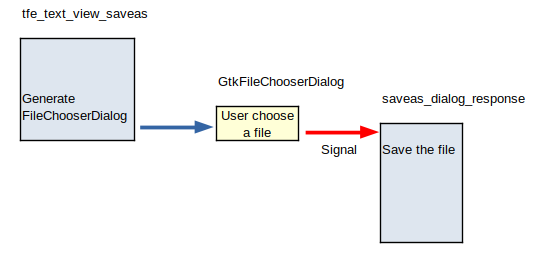
\includegraphics[width=10.7cm,height=5.16cm]{../image/saveas.png}
\caption{Saveas process}
\end{figure}

When you use GtkFileChooserDialog, you need to divide the program into
two parts. One is a function which creates GtkFileChooserDialog and the
other is a signal handler. The function just creates and shows
GtkFileChooserDialog. The rest is done by the handler. It gets Gfile
from GtkFileChooserDialog and saves the buffer to the file by calling
\passthrough{\lstinline!save\_file!}.

\hypertarget{open-function}{%
\subsection{Open function}\label{open-function}}

Open function shows GtkFileChooserDialog to users and prompts them to
choose a file. Then it reads the file and puts the text into
GtkTextBuffer.

\begin{lstlisting}[language=C]
void tfe_text_view_open (TfeTextView *tv, GtkWindow *win);
\end{lstlisting}

The parameter \passthrough{\lstinline!win!} is the top-level window. It
will be a transient parent window of GtkFileChooserDialog when the
dialog is created. This allows window managers to keep the dialog on top
of the parent window, or center the dialog over the parent window. It is
possible to give no parent window to the dialog. However, it is
encouraged to give a parent window to dialog. This function might be
called just after \passthrough{\lstinline!tv!} has been created. In that
case, \passthrough{\lstinline!tv!} has not been incorporated into the
widget hierarchy. Therefore it is impossible to get the top-level window
from \passthrough{\lstinline!tv!}. That's why the function needs
\passthrough{\lstinline!win!} parameter.

This function is usually called when the buffer of
\passthrough{\lstinline!tv!} is empty. However, even if the buffer is
not empty, \passthrough{\lstinline!tfe\_text\_view\_open!} doesn't treat
it as an error. If you want to revert the buffer, calling this function
is appropriate. Otherwise probably bad things will happen.

\begin{lstlisting}[language=C, numbers=left]
static void
open_dialog_response(GtkWidget *dialog, gint response, TfeTextView *tv) {
  GtkTextBuffer *tb = gtk_text_view_get_buffer (GTK_TEXT_VIEW (tv));
  GFile *file;
  char *contents;
  gsize length;
  GtkWidget *message_dialog;
  GError *err = NULL;

  if (response != GTK_RESPONSE_ACCEPT)
    g_signal_emit (tv, tfe_text_view_signals[OPEN_RESPONSE], 0, TFE_OPEN_RESPONSE_CANCEL);
  else if (! G_IS_FILE (file = gtk_file_chooser_get_file (GTK_FILE_CHOOSER (dialog)))) {
    g_warning ("TfeTextView: gtk_file_chooser_get_file returns non GFile.\n");
    g_signal_emit (tv, tfe_text_view_signals[OPEN_RESPONSE], 0, TFE_OPEN_RESPONSE_ERROR);
  } else if (! g_file_load_contents (file, NULL, &contents, &length, NULL, &err)) { /* read error */
    g_object_unref (file);
    message_dialog = gtk_message_dialog_new (GTK_WINDOW (dialog), GTK_DIALOG_MODAL,
                                             GTK_MESSAGE_ERROR, GTK_BUTTONS_CLOSE,
                                            "%s.\n", err->message);
    g_signal_connect (message_dialog, "response", G_CALLBACK (gtk_window_destroy), NULL);
    gtk_widget_show (message_dialog);
    g_error_free (err);
    g_signal_emit (tv, tfe_text_view_signals[OPEN_RESPONSE], 0, TFE_OPEN_RESPONSE_ERROR);
  } else {
    gtk_text_buffer_set_text (tb, contents, length);
    g_free (contents);
    if (G_IS_FILE (tv->file))
      g_object_unref (tv->file);
    tv->file = file;
    gtk_text_buffer_set_modified (tb, FALSE);
    g_signal_emit (tv, tfe_text_view_signals[OPEN_RESPONSE], 0, TFE_OPEN_RESPONSE_SUCCESS);
    g_signal_emit (tv, tfe_text_view_signals[CHANGE_FILE], 0);
  }
  gtk_window_destroy (GTK_WINDOW (dialog));
}

void
tfe_text_view_open (TfeTextView *tv, GtkWindow *win) {
  g_return_if_fail (TFE_IS_TEXT_VIEW (tv));
  g_return_if_fail (GTK_IS_WINDOW (win));

  GtkWidget *dialog;

  dialog = gtk_file_chooser_dialog_new ("Open file", win, GTK_FILE_CHOOSER_ACTION_OPEN,
                                        "Cancel", GTK_RESPONSE_CANCEL,
                                        "Open", GTK_RESPONSE_ACCEPT,
                                        NULL);
  g_signal_connect (dialog, "response", G_CALLBACK (open_dialog_response), tv);
  gtk_widget_show (dialog);
}
\end{lstlisting}

\begin{itemize}
\tightlist
\item
  37-50: \passthrough{\lstinline!tfe\_text\_view\_open!} function.
\item
  44-47: Creates GtkFileChooserDialog. The title is ``Open file''.
  Transient parent window is the top-level window of the application,
  which is given by the caller. The action is open mode. The buttons are
  Cancel and Open.
\item
  48: connects the ``response'' signal of the dialog and
  \passthrough{\lstinline!open\_dialog\_response!} signal handler.
\item
  49: Shows the dialog.
\item
  1-35: \passthrough{\lstinline!open\_dialog\_response!} signal handler.
\item
  10-11: If the response from GtkFileChooserDialog is not
  \passthrough{\lstinline!GTK\_RESPONSE\_ACCEPT!}, the user has clicked
  on the ``Cancel'' button or close button on the header bar. Then,
  ``open-response'' signal is emitted. The parameter of the signal is
  \passthrough{\lstinline!TFE\_OPEN\_RESPONSE\_CANCEL!}.
\item
  12-14: Gets the pointer to the Gfile by
  \passthrough{\lstinline!gtk\_file\_chooser\_get\_file!}. If it doesn't
  point GFile, maybe an error has occurred. Then it emits
  ``open-response'' signal with the parameter
  \passthrough{\lstinline!TFE\_OPEN\_RESPONSE\_ERROR!}.
\item
  15-23: If an error occurs at file reading, then it decreases the
  reference count of the Gfile, shows a message dialog to report the
  error to the user and emits ``open-response'' signal with the
  parameter \passthrough{\lstinline!TFE\_OPEN\_RESPONSE\_ERROR!}.
\item
  24-33: If the file has successfully been read, then the text is
  inserted to GtkTextBuffer, frees the temporary buffer pointed by
  \passthrough{\lstinline!contents!} and sets
  \passthrough{\lstinline!tv->file!} to point the file (no duplication
  is not necessary). Then, it emits ``open-response'' signal with the
  parameter \passthrough{\lstinline!TFE\_OPEN\_RESPONSE\_SUCCESS!} and
  emits ``change-file'' signal.
\item
  34: destroys GtkFileCooserDialog.
\end{itemize}

Now let's think about the whole process between the caller and
TfeTextView. It is shown in the following diagram and you would think
that it is really complicated. Because signal is the only way for
GtkFileChooserDialog to communicate with others. In Gtk3,
\passthrough{\lstinline!gtk\_dialog\_run!} function is available. It
simplifies the process. However, in Gtk4,
\passthrough{\lstinline!gtk\_dialog\_run!} is unavailable any more.

\begin{figure}
\centering
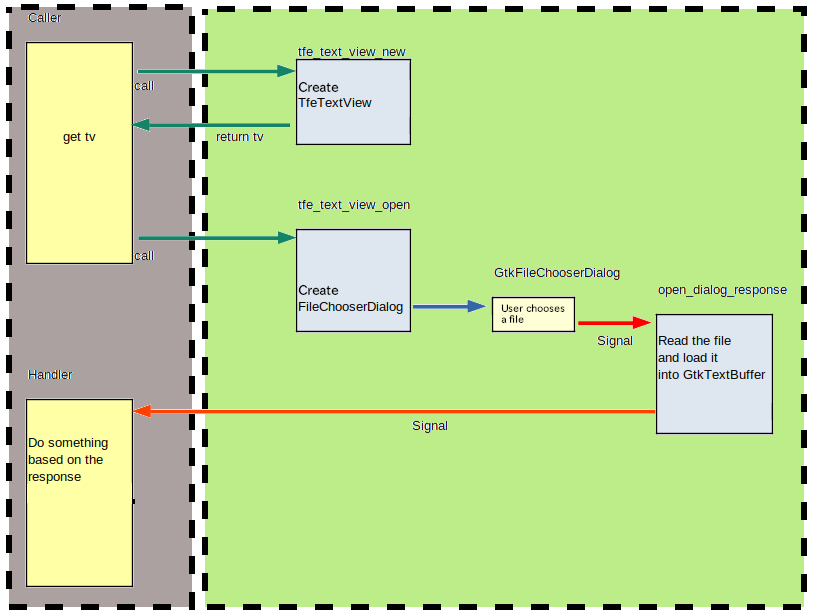
\includegraphics[width=12.405cm,height=9.225cm]{../image/open.png}
\caption{Caller and TfeTextView}
\end{figure}

\begin{enumerate}
\def\labelenumi{\arabic{enumi}.}
\tightlist
\item
  A caller gets a pointer \passthrough{\lstinline!tv!} to a TfeTextView
  instance by calling \passthrough{\lstinline!tfe\_text\_view\_new!}.
\item
  The caller connects the handler (left bottom in the diagram) and the
  signal ``open-response''.
\item
  It calls \passthrough{\lstinline!tfe\_text\_view\_open!} to prompt the
  user to select a file from GtkFileChooserDialog.
\item
  The dialog emits a signal and it invokes the handler
  \passthrough{\lstinline!open\_dialog\_response!}.
\item
  The handler reads the file and inserts the text into GtkTextBuffer and
  emits a signal to inform the status as a response code.
\item
  The handler out of the TfeTextView receives the signal.
\end{enumerate}

\hypertarget{getting-gfile}{%
\subsection{Getting Gfile}\label{getting-gfile}}

\passthrough{\lstinline!gtk\_text\_view\_get\_file!} is a simple
function shown as follows.

\begin{lstlisting}[language=C, numbers=left]
GFile *
tfe_text_view_get_file (TfeTextView *tv) {
  g_return_val_if_fail (TFE_IS_TEXT_VIEW (tv), NULL);

  if (G_IS_FILE (tv->file))
    return g_file_dup (tv->file);
  else
    return NULL;
}
\end{lstlisting}

The important thing is to duplicate \passthrough{\lstinline!tv->file!}.
Otherwise, if the caller frees the GFile object,
\passthrough{\lstinline!tv->file!} is no more guaranteed to point the
GFile. Another reason to use \passthrough{\lstinline!g\_file\_dup!} is
that GFile isn't thread-safe. If you use GFile in the different thread,
the duplication is necessary. See
\href{https://docs.gtk.org/gio/method.File.dup.html}{Gio API Reference,
g\_file\_dup}.

\hypertarget{the-api-document-and-source-file-of-tfetextview.c}{%
\subsection{The API document and source file of
tfetextview.c}\label{the-api-document-and-source-file-of-tfetextview.c}}

Refer API document of TfeTextView in the appendix. Its original markdown
file is under the directory \passthrough{\lstinline!src/tfetextview!}.

All the source files are listed in Section 16. You can find them under
src/tfe5 and src/tfetextview directories.

  \hypertarget{functions-in-gtknotebook}{%
\section{Functions in GtkNotebook}\label{functions-in-gtknotebook}}

GtkNotebook is a very important object in the text file editor
\passthrough{\lstinline!tfe!}. It connects the application and
TfeTextView objects. A set of public functions are declared in
\passthrough{\lstinline!tfenotebook.h!}. The word ``tfenotebook'' is
used only in filenames. There's no ``TfeNotebook'' object.

\begin{lstlisting}[language=C, numbers=left]
void
notebook_page_save(GtkNotebook *nb);

void
notebook_page_close (GtkNotebook *nb);

void
notebook_page_open (GtkNotebook *nb);

void
notebook_page_new_with_file (GtkNotebook *nb, GFile *file);

void
notebook_page_new (GtkNotebook *nb);
\end{lstlisting}

This header file describes the public functions in
\passthrough{\lstinline!tfenotebook.c!}.

\begin{itemize}
\tightlist
\item
  1-2: \passthrough{\lstinline!notebook\_page\_save!} saves the current
  page to the file of which the name specified in the tab. If the name
  is \passthrough{\lstinline!untitled!} or
  \passthrough{\lstinline!untitled!} followed by digits,
  FileChooserDialog appears and a user can choose or specify a filename.
\item
  4-5: \passthrough{\lstinline!notebook\_page\_close!} closes the
  current page.
\item
  7-8: \passthrough{\lstinline!notebook\_page\_open!} shows a file
  chooser dialog and a user can choose a file. The file is inserted to a
  new page.
\item
  10-11: \passthrough{\lstinline!notebook\_page\_new\_with\_file!}
  creates a new page and the file given as an argument is read and
  inserted into the page.
\item
  13-14: \passthrough{\lstinline!notebook\_page\_new!} creates a new
  empty page.
\end{itemize}

You probably find that the functions except
\passthrough{\lstinline!notebook\_page\_close!} are higher level
functions of

\begin{itemize}
\tightlist
\item
  \passthrough{\lstinline!tfe\_text\_view\_save!}
\item
  \passthrough{\lstinline!tef\_text\_view\_open!}
\item
  \passthrough{\lstinline!tfe\_text\_view\_new\_with\_file!}
\item
  \passthrough{\lstinline!tfe\_text\_view\_new!}
\end{itemize}

respectively.

There are two layers. One of them is
\passthrough{\lstinline!tfe\_text\_view ...!}, which is the lower level
layer. The other is \passthrough{\lstinline!note\_book ...!}, which is
the higher level layer.

Now let's look at the program of each function.

\hypertarget{notebook_page_new}{%
\subsection{notebook\_page\_new}\label{notebook_page_new}}

\begin{lstlisting}[language=C, numbers=left]
static gchar*
get_untitled () {
  static int c = -1;
  if (++c == 0) 
    return g_strdup_printf("Untitled");
  else
    return g_strdup_printf ("Untitled%u", c);
}

static void
notebook_page_build (GtkNotebook *nb, GtkWidget *tv, char *filename) {
  GtkWidget *scr = gtk_scrolled_window_new ();
  GtkNotebookPage *nbp;
  GtkWidget *lab;
  int i;

  gtk_text_view_set_wrap_mode (GTK_TEXT_VIEW (tv), GTK_WRAP_WORD_CHAR);
  gtk_scrolled_window_set_child (GTK_SCROLLED_WINDOW (scr), tv);
  lab = gtk_label_new (filename);
  i = gtk_notebook_append_page (nb, scr, lab);
  nbp = gtk_notebook_get_page (nb, scr);
  g_object_set (nbp, "tab-expand", TRUE, NULL);
  gtk_notebook_set_current_page (nb, i);
  g_signal_connect (GTK_TEXT_VIEW (tv), "change-file", G_CALLBACK (file_changed_cb), nb);
}

void
notebook_page_new (GtkNotebook *nb) {
  g_return_if_fail(GTK_IS_NOTEBOOK (nb));

  GtkWidget *tv;
  char *filename;

  if ((tv = tfe_text_view_new ()) == NULL)
    return;
  filename = get_untitled ();
  notebook_page_build (nb, tv, filename);
}
\end{lstlisting}

\begin{itemize}
\tightlist
\item
  27-38: \passthrough{\lstinline!notebook\_page\_new!} function.
\item
  29: \passthrough{\lstinline!g\_return\_if\_fail!} is used to check the
  argument.
\item
  34: Creates TfeTextView object. If it fails, it returns to the caller.
\item
  36: Creates filename, which is ``Untitled'', ``Untitled1'', \ldots{} .
\item
  1-8: \passthrough{\lstinline!get\_untitled!} function.
\item
  3: Static variable \passthrough{\lstinline!c!} is initialized at the
  first call of this function. After that \passthrough{\lstinline!c!}
  keeps its value unless it is changed explicitly.
\item
  4-7: Increases \passthrough{\lstinline!c!} by one and if it is zero
  then it returns ``Untitled''. If it is a positive integer then it
  returns ``Untitled\textless the integer\textgreater{}'', for example,
  ``Untitled1'', ``Untitled2'', and so on. The function
  \passthrough{\lstinline!g\_strdup\_printf!} creates a string and it
  should be freed by \passthrough{\lstinline!g\_free!} when it becomes
  useless. The caller of \passthrough{\lstinline!get\_untitled!} is in
  charge of freeing the string.
\item
  37: calls \passthrough{\lstinline!notebook\_page\_build!} to build the
  contents of the page.
\item
  10- 25: \passthrough{\lstinline!notebook\_page\_build!} function.
\item
  12: Creates GtkScrolledWindow.
\item
  17: Sets the wrap mode of \passthrough{\lstinline!tv!} to
  GTK\_WRAP\_WORD\_CHAR so that lines are broken between words or
  graphemes.
\item
  18: Inserts \passthrough{\lstinline!tv!} to GtkscrolledWindow as a
  child.
\item
  19-20: Creates GtkLabel, then appends \passthrough{\lstinline!scr!}
  and \passthrough{\lstinline!lab!} to the GtkNotebook instance
  \passthrough{\lstinline!nb!}.
\item
  21-22: Sets ``tab-expand'' property to TRUE. The function
  \passthrough{\lstinline!g\_object\_set!} sets properties on an object.
  The object is any object derived from GObject. In many cases, an
  object has its own function to set its properties, but sometimes not.
  In that case, use \passthrough{\lstinline!g\_object\_set!} to set the
  property.
\item
  23: Sets the current page of \passthrough{\lstinline!nb!} to the newly
  created page.
\item
  24: Connects ``change-file'' signal and
  \passthrough{\lstinline!file\_changed\_cb!} handler.
\end{itemize}

\hypertarget{notebook_page_new_with_file}{%
\subsection{notebook\_page\_new\_with\_file}\label{notebook_page_new_with_file}}

\begin{lstlisting}[language=C, numbers=left]
void
notebook_page_new_with_file (GtkNotebook *nb, GFile *file) {
  g_return_if_fail(GTK_IS_NOTEBOOK (nb));
  g_return_if_fail(G_IS_FILE (file));

  GtkWidget *tv;
  char *filename;

  if ((tv = tfe_text_view_new_with_file (file)) == NULL)
    return; /* read error */
  filename = g_file_get_basename (file);
  notebook_page_build (nb, tv, filename);
}
\end{lstlisting}

\begin{itemize}
\tightlist
\item
  9-10: Calls
  \passthrough{\lstinline!tfe\_text\_view\_new\_with\_file!}. If the
  function returns NULL, an error has happend. Then, it does nothing and
  returns.
\item
  11-12: Gets the filename and builds the contents of the page.
\end{itemize}

\hypertarget{notebook_page_open}{%
\subsection{notebook\_page\_open}\label{notebook_page_open}}

\begin{lstlisting}[language=C, numbers=left]
static void
open_response (TfeTextView *tv, int response, GtkNotebook *nb) {
  GFile *file;
  char *filename;

  if (response != TFE_OPEN_RESPONSE_SUCCESS || ! G_IS_FILE (file = tfe_text_view_get_file (tv))) {
    g_object_ref_sink (tv);
    g_object_unref (tv);
  }else {
    filename = g_file_get_basename (file);
    g_object_unref (file);
    notebook_page_build (nb, GTK_WIDGET (tv), filename);
  }
}

void
notebook_page_open (GtkNotebook *nb) {
  g_return_if_fail(GTK_IS_NOTEBOOK (nb));

  GtkWidget *tv;

  if ((tv = tfe_text_view_new ()) == NULL)
    return;
  g_signal_connect (TFE_TEXT_VIEW (tv), "open-response", G_CALLBACK (open_response), nb);
  tfe_text_view_open (TFE_TEXT_VIEW (tv), GTK_WINDOW (gtk_widget_get_ancestor (GTK_WIDGET (nb), GTK_TYPE_WINDOW)));
}
\end{lstlisting}

\begin{itemize}
\tightlist
\item
  16-26: \passthrough{\lstinline!notebook\_page\_open!} function.
\item
  22-23: Creates TfeTextView object. If NULL is returned, an error has
  happened. Then, it returns to the caller.
\item
  24: Connects the signal ``open-response'' and the handler
  \passthrough{\lstinline!open\_response!}.
\item
  25: Calls \passthrough{\lstinline!tfe\_text\_view\_open!}. The
  ``open-response'' signal will be emitted later to inform the result of
  opening and reading a file.
\item
  1-14: \passthrough{\lstinline!open\_response!} handler.
\item
  6-8: If the response code is NOT
  \passthrough{\lstinline!TFE\_OPEN\_RESPONSE\_SUCCESS!} or
  \passthrough{\lstinline!tfe\_text\_view\_get\_file!} doesn't return
  the pointer to a GFile, it has failed to open and read a new file.
  Then, what \passthrough{\lstinline!notebook\_page\_open!} did in
  advance need to be canceled. The instance \passthrough{\lstinline!tv!}
  hasn't been a child widget of GtkScrolledWindow yet. Such instance has
  floating reference. Floating reference will be explained later in this
  subsection. You need to call
  \passthrough{\lstinline!g\_object\_ref\_sink!} first. Then the
  floating reference is converted into an ordinary reference. Now you
  call \passthrough{\lstinline!g\_object\_unref!} to decrease the
  reference count by one.
\item
  9-13: Otherwise, everything is okay. Gets the filename, builds the
  contents of the page.
\end{itemize}

All the widgets are derived from GInitiallyUnowned. When an instance of
GInitiallyUnowned or its descendant is created, the instance has a
floating reference. The function
\passthrough{\lstinline!g\_object\_ref\_sink!} converts the floating
reference into an ordinary reference. If the instance doesn't have a
floating reference, \passthrough{\lstinline!g\_object\_ref\_sink!}
simply increases the reference count by one. On the other hand, when an
instance of GObject (not GInitiallyUnowned) is created, no floating
reference is given. And the instance has a normal reference count
instead of floating reference.

If you use \passthrough{\lstinline!g\_object\_unref!} to an instance
that has a floating reference, you need to convert the floating
reference to a normal reference in advance. See
\href{https://developer-old.gnome.org/gobject/stable/gobject-The-Base-Object-Type.html\#gobject-The-Base-Object-Type.description}{GObject
Reference Manual} for further information.

\hypertarget{notebook_page_close}{%
\subsection{notebook\_page\_close}\label{notebook_page_close}}

\begin{lstlisting}[language=C, numbers=left]
void
notebook_page_close (GtkNotebook *nb) {
  g_return_if_fail(GTK_IS_NOTEBOOK (nb));

  GtkWidget *win;
  int i;

  if (gtk_notebook_get_n_pages (nb) == 1) {
    win = gtk_widget_get_ancestor (GTK_WIDGET (nb), GTK_TYPE_WINDOW);
    gtk_window_destroy(GTK_WINDOW (win));
  } else {
    i = gtk_notebook_get_current_page (nb);
    gtk_notebook_remove_page (GTK_NOTEBOOK (nb), i);
  }
}
\end{lstlisting}

This function closes the current page. If the page is the only page the
notebook has, then the function destroys the top-level window and quits
the application.

\begin{itemize}
\tightlist
\item
  8-10: If the page is the only page the notebook has, it calls
  \passthrough{\lstinline!gtk\_window\_destroy!} to destroys the
  top-level window.
\item
  11-13: Otherwise, removes the current page.
\end{itemize}

\hypertarget{notebook_page_save}{%
\subsection{notebook\_page\_save}\label{notebook_page_save}}

\begin{lstlisting}[language=C, numbers=left]
static TfeTextView *
get_current_textview (GtkNotebook *nb) {
  int i;
  GtkWidget *scr;
  GtkWidget *tv;

  i = gtk_notebook_get_current_page (nb);
  scr = gtk_notebook_get_nth_page (nb, i);
  tv = gtk_scrolled_window_get_child (GTK_SCROLLED_WINDOW (scr));
  return TFE_TEXT_VIEW (tv);
}

void
notebook_page_save (GtkNotebook *nb) {
  g_return_if_fail(GTK_IS_NOTEBOOK (nb));

  TfeTextView *tv;

  tv = get_current_textview (nb);
  tfe_text_view_save (TFE_TEXT_VIEW (tv));
}
\end{lstlisting}

\begin{itemize}
\tightlist
\item
  13-21: \passthrough{\lstinline!notebook\_page\_save!}.
\item
  19: Gets TfeTextView belongs to the current page.
\item
  20: Calls \passthrough{\lstinline!tfe\_text\_view\_save!}.
\item
  1-11: \passthrough{\lstinline!get\_current\_textview!}. This function
  gets the TfeTextView object belongs to the current page.
\item
  7: Gets the page number of the current page.
\item
  8: Gets the child widget \passthrough{\lstinline!scr!}, which is a
  GtkScrolledWindow instance, of the current page.
\item
  9-10: Gets the child widget of \passthrough{\lstinline!scr!}, which is
  a TfeTextView instance, and returns it.
\end{itemize}

\hypertarget{file_changed_cb-handler}{%
\subsection{file\_changed\_cb handler}\label{file_changed_cb-handler}}

The function \passthrough{\lstinline!file\_changed\_cb!} is a handler
connected to ``change-file'' signal. If a file in a TfeTextView instance
is changed, it emits this signal. This handler changes the label of
GtkNotebookPage.

\begin{lstlisting}[language=C, numbers=left]
static void
file_changed_cb (TfeTextView *tv, GtkNotebook *nb) {
  GtkWidget *scr;
  GtkWidget *label;
  GFile *file;
  char *filename;

  file = tfe_text_view_get_file (tv);
  scr = gtk_widget_get_parent (GTK_WIDGET (tv));
  if (G_IS_FILE (file)) {
    filename = g_file_get_basename (file);
    g_object_unref (file);
  } else
    filename = get_untitled ();
  label = gtk_label_new (filename);
  g_free (filename);
  gtk_notebook_set_tab_label (nb, scr, label);
}
\end{lstlisting}

\begin{itemize}
\tightlist
\item
  8: Gets the GFile instance from \passthrough{\lstinline!tv!}.
\item
  9: Gets the GkScrolledWindow instance which is the parent widget of
  \passthrough{\lstinline!tv!}.
\item
  10-12: If \passthrough{\lstinline!file!} points GFile, then assigns
  the filename of the GFile into \passthrough{\lstinline!filename!}.
  Then, unref the GFile object \passthrough{\lstinline!file!}.
\item
  13-14: Otherwise (file is NULL), assigns untitled string to
  \passthrough{\lstinline!filename!}.
\item
  15-16: Creates a GtkLabel instance \passthrough{\lstinline!label!}
  with the filename and set the label of the GtkNotebookPage with
  \passthrough{\lstinline!label!}.
\end{itemize}

  \hypertarget{tfeapplication.c}{%
\section{tfeapplication.c}\label{tfeapplication.c}}

\passthrough{\lstinline!tfeapplication.c!} includes all the code other
than \passthrough{\lstinline!tfetxtview.c!} and
\passthrough{\lstinline!tfenotebook.c!}. It does:

\begin{itemize}
\tightlist
\item
  Application support, mainly handling command line arguments.
\item
  Builds widgets using ui file.
\item
  Connects button signals and their handlers.
\item
  Manages CSS.
\end{itemize}

\hypertarget{main}{%
\subsection{main}\label{main}}

The function \passthrough{\lstinline!main!} is the first invoked
function in C language. It connects the command line given by the user
and Gtk application.

\begin{lstlisting}[language=C, numbers=left]
#define APPLICATION_ID "com.github.ToshioCP.tfe"

int
main (int argc, char **argv) {
  GtkApplication *app;
  int stat;

  app = gtk_application_new (APPLICATION_ID, G_APPLICATION_HANDLES_OPEN);

  g_signal_connect (app, "startup", G_CALLBACK (app_startup), NULL);
  g_signal_connect (app, "activate", G_CALLBACK (app_activate), NULL);
  g_signal_connect (app, "open", G_CALLBACK (app_open), NULL);

  stat =g_application_run (G_APPLICATION (app), argc, argv);
  g_object_unref (app);
  return stat;
}
\end{lstlisting}

\begin{itemize}
\tightlist
\item
  1: Defines the application id. It is easy to find the application id,
  and better than the id is embedded in
  \passthrough{\lstinline!gtk\_application\_new!}.
\item
  8: Creates GtkApplication object.
\item
  10-12: Connects ``startup'', ``activate'' and ``open'' signals to
  their handlers.
\item
  14: Runs the application.
\item
  15-16: releases the reference to the application and returns the
  status.
\end{itemize}

\hypertarget{startup-signal-handler}{%
\subsection{startup signal handler}\label{startup-signal-handler}}

Startup signal is emitted just after the GtkApplication instance is
initialized. What the signal handler needs to do is initialization of
the application.

\begin{itemize}
\tightlist
\item
  Builds the widgets using ui file.
\item
  Connects button signals and their handlers.
\item
  Sets CSS.
\end{itemize}

The handler is as follows.

\begin{lstlisting}[language=C, numbers=left]
static void
app_startup (GApplication *application) {
  GtkApplication *app = GTK_APPLICATION (application);
  GtkBuilder *build;
  GtkApplicationWindow *win;
  GtkNotebook *nb;
  GtkButton *btno;
  GtkButton *btnn;
  GtkButton *btns;
  GtkButton *btnc;

  build = gtk_builder_new_from_resource ("/com/github/ToshioCP/tfe/tfe.ui");
  win = GTK_APPLICATION_WINDOW (gtk_builder_get_object (build, "win"));
  nb = GTK_NOTEBOOK (gtk_builder_get_object (build, "nb"));
  gtk_window_set_application (GTK_WINDOW (win), app);
  btno = GTK_BUTTON (gtk_builder_get_object (build, "btno"));
  btnn = GTK_BUTTON (gtk_builder_get_object (build, "btnn"));
  btns = GTK_BUTTON (gtk_builder_get_object (build, "btns"));
  btnc = GTK_BUTTON (gtk_builder_get_object (build, "btnc"));
  g_signal_connect_swapped (btno, "clicked", G_CALLBACK (open_cb), nb);
  g_signal_connect_swapped (btnn, "clicked", G_CALLBACK (new_cb), nb);
  g_signal_connect_swapped (btns, "clicked", G_CALLBACK (save_cb), nb);
  g_signal_connect_swapped (btnc, "clicked", G_CALLBACK (close_cb), nb);
  g_object_unref(build);

GdkDisplay *display;

  display = gtk_widget_get_display (GTK_WIDGET (win));
  GtkCssProvider *provider = gtk_css_provider_new ();
  gtk_css_provider_load_from_data (provider, "textview {padding: 10px; font-family: monospace; font-size: 12pt;}", -1);
  gtk_style_context_add_provider_for_display (display, GTK_STYLE_PROVIDER (provider), GTK_STYLE_PROVIDER_PRIORITY_APPLICATION);
}
\end{lstlisting}

\begin{itemize}
\tightlist
\item
  12-15: Builds widgets using ui file (resource). Connects the top-level
  window and the application with
  \passthrough{\lstinline!gtk\_window\_set\_application!}.
\item
  16-23: Gets buttons and connects their signals and handlers.
\item
  24: Releases the reference to GtkBuilder.
\item
  26-31: Sets CSS. CSS in Gtk is similar to CSS in HTML. You can set
  margin, border, padding, color, font and so on with CSS. In this
  program CSS is in line 30. It sets padding, font-family and font size
  of GtkTextView.
\item
  26-28: GdkDisplay is used to set CSS. CSS will be explained in the
  next subsection.
\end{itemize}

\hypertarget{css-in-gtk}{%
\subsection{CSS in Gtk}\label{css-in-gtk}}

CSS is an abbreviation of Cascading Style Sheet. It is originally used
with HTML to describe the presentation semantics of a document. You
might have found that the widgets in Gtk is similar to a window in a
browser. It implies that CSS can also be applied to Gtk windowing
system.

\hypertarget{css-nodes-selectors}{%
\subsubsection{CSS nodes, selectors}\label{css-nodes-selectors}}

The syntax of CSS is as follows.

\begin{lstlisting}
selector { color: yellow; padding-top: 10px; ...}
\end{lstlisting}

Every widget has CSS node. For example GtkTextView has
\passthrough{\lstinline!textview!} node. If you want to set style to
GtkTextView, substitute ``textview'' for the selector.

\begin{lstlisting}
textview {color: yellow; ...}
\end{lstlisting}

Class, ID and some other things can be applied to the selector like Web
CSS. Refer to \href{https://docs.gtk.org/gtk4/css-overview.html}{Gtk4
API Reference, CSS in Gtk} for further information.

In line 30, the CSS is a string.

\begin{lstlisting}
textview {padding: 10px; font-family: monospace; font-size: 12pt;}
\end{lstlisting}

\begin{itemize}
\tightlist
\item
  padding is a space between the border and contents. This space makes
  the textview easier to read.
\item
  font-family is a name of font. ``monospace'' is one of the generic
  family font keywords.
\item
  font-size is set to 12pt.
\end{itemize}

\hypertarget{gtkstylecontext-gtkcssprovider-and-gdkdisplay}{%
\subsubsection{GtkStyleContext, GtkCSSProvider and
GdkDisplay}\label{gtkstylecontext-gtkcssprovider-and-gdkdisplay}}

GtkStyleContext is an object that stores styling information affecting a
widget. Each widget is connected to the corresponding GtkStyleContext.
You can get the context by
\passthrough{\lstinline!gtk\_widget\_get\_style\_context!}.

GtkCssProvider is an object which parses CSS in order to style widgets.

To apply your CSS to widgets, you need to add GtkStyleProvider (the
interface of GtkCSSProvider) to GtkStyleContext. However, instead, you
can add it to GdkDisplay of the window (usually top-level window).

Look at the source file of \passthrough{\lstinline!startup!} handler
again.

\begin{itemize}
\tightlist
\item
  28: The display is obtained by
  \passthrough{\lstinline!gtk\_widget\_get\_display!}.
\item
  29: Creates a GtkCssProvider instance.
\item
  30: Puts the CSS into the provider.
\item
  31: Adds the provider to the display. The last argument of
  \passthrough{\lstinline!gtk\_style\_context\_add\_provider\_for\_display!}
  is the priority of the style provider.
  \passthrough{\lstinline!GTK\_STYLE\_PROVIDER\_PRIORITY\_APPLICATION!}
  is a priority for application-specific style information.
  \passthrough{\lstinline!GTK\_STYLE\_PROVIDER\_PRIORITY\_USER!} is also
  often used and it is the highest priority. So,
  \passthrough{\lstinline!GTK\_STYLE\_PROVIDER\_PRIORITY\_USER!} is
  often used to a specific widget.
\end{itemize}

It is possible to add the provider to the context of GtkTextView instead
of GdkDiplay. To do so, rewrite
\passthrough{\lstinline!tfe\_text\_view\_new!}. First, get the
GtkStyleContext object of a TfeTextView object. Then adds the CSS
provider to the context.

\begin{lstlisting}[language=C]
GtkWidget *
tfe_text_view_new (void) {
  GtkWidget *tv;

  tv = gtk_widget_new (TFE_TYPE_TEXT_VIEW, NULL);

  GtkStyleContext *context;

  context = gtk_widget_get_style_context (GTK_WIDGET (tv));
  GtkCssProvider *provider = gtk_css_provider_new ();
  gtk_css_provider_load_from_data (provider, "textview {padding: 10px; font-family: monospace; font-size: 12pt;}", -1);
  gtk_style_context_add_provider (context, GTK_STYLE_PROVIDER (provider), GTK_STYLE_PROVIDER_PRIORITY_USER);

  return tv;
}
\end{lstlisting}

CSS in the context takes precedence over CSS in the display.

\hypertarget{activate-and-open-handler}{%
\subsection{activate and open handler}\label{activate-and-open-handler}}

The handler of ``activate'' and ``open'' signal are
\passthrough{\lstinline!app\_activate!} and
\passthrough{\lstinline!app\_open!} respectively. They just create a new
GtkNotebookPage.

\begin{lstlisting}[language=C, numbers=left]
static void
app_activate (GApplication *application) {
  GtkApplication *app = GTK_APPLICATION (application);
  GtkWidget *win = GTK_WIDGET (gtk_application_get_active_window (app));
  GtkWidget *boxv = gtk_window_get_child (GTK_WINDOW (win));
  GtkNotebook *nb = GTK_NOTEBOOK (gtk_widget_get_last_child (boxv));

  notebook_page_new (nb);
  gtk_widget_show (GTK_WIDGET (win));
}

static void
app_open (GApplication *application, GFile ** files, gint n_files, const gchar *hint) {
  GtkApplication *app = GTK_APPLICATION (application);
  GtkWidget *win = GTK_WIDGET (gtk_application_get_active_window (app));
  GtkWidget *boxv = gtk_window_get_child (GTK_WINDOW (win));
  GtkNotebook *nb = GTK_NOTEBOOK (gtk_widget_get_last_child (boxv));
  int i;

  for (i = 0; i < n_files; i++)
    notebook_page_new_with_file (nb, files[i]);
  if (gtk_notebook_get_n_pages (nb) == 0)
    notebook_page_new (nb);
  gtk_widget_show (win);
}
\end{lstlisting}

\begin{itemize}
\tightlist
\item
  1-10: \passthrough{\lstinline!app\_activate!}.
\item
  8-10: Creates a new page and shows the window.
\item
  12-25: \passthrough{\lstinline!app\_open!}.
\item
  20-21: Creates notebook pages with files.
\item
  22-23: If no page has created, maybe because of read error, then it
  creates an empty page.
\item
  24: Shows the window.
\end{itemize}

These codes have become really simple thanks to tfenotebook.c and
tfetextview.c.

\hypertarget{primary-instance}{%
\subsection{Primary instance}\label{primary-instance}}

Only one GApplication instance can be run at a time per session. The
session is a bit difficult concept and also platform-dependent, but
roughly speaking, it corresponds to a graphical desktop login. When you
use your PC, you probably login first, then your desktop appears until
you log off. This is the session.

However, Linux is multi process OS and you can run two or more instances
of the same application. Isn't it a contradiction?

When first instance is launched, then it registers itself with its
application ID (for example,
\passthrough{\lstinline!com.github.ToshioCP.tfe!}). Just after the
registration, startup signal is emitted, then activate or open signal is
emitted and the instance's main loop runs. I wrote ``startup signal is
emitted just after the application instance is initialized'' in the
prior subsection. More precisely, it is emitted just after the
registration.

If another instance which has the same application ID is invoked, it
also tries to register itself. Because this is the second instance, the
registration of the ID has already done, so it fails. Because of the
failure startup signal isn't emitted. After that, activate or open
signal is emitted in the primary instance, not the second instance. The
primary instance receives the signal and its handler is invoked. On the
other hand, the second instance doesn't receive the signal and it
immediately quits.

Try to run two instances in a row.

\begin{lstlisting}
$ ./_build/tfe &
[1] 84453
$ ./build/tfe tfeapplication.c
$
\end{lstlisting}

First, the primary instance opens a window. Then, after the second
instance is run, a new notebook page with the contents of
\passthrough{\lstinline!tfeapplication.c!} appears in the primary
instance's window. This is because the open signal is emitted in the
primary instance. The second instance immediately quits so shell prompt
soon appears.

\hypertarget{a-series-of-handlers-correspond-to-the-button-signals}{%
\subsection{a series of handlers correspond to the button
signals}\label{a-series-of-handlers-correspond-to-the-button-signals}}

\begin{lstlisting}[language=C, numbers=left]
static void
open_cb (GtkNotebook *nb) {
  notebook_page_open (nb);
}

static void
new_cb (GtkNotebook *nb) {
  notebook_page_new (nb);
}

static void
save_cb (GtkNotebook *nb) {
  notebook_page_save (nb);
}

static void
close_cb (GtkNotebook *nb) {
  notebook_page_close (GTK_NOTEBOOK (nb));
}
\end{lstlisting}

\passthrough{\lstinline!open\_cb!}, \passthrough{\lstinline!new\_cb!},
\passthrough{\lstinline!save\_cb!} and
\passthrough{\lstinline!close\_cb!} just call corresponding notebook
page functions.

\hypertarget{meson.build}{%
\subsection{meson.build}\label{meson.build}}

\begin{lstlisting}[numbers=left]
project('tfe', 'c')

gtkdep = dependency('gtk4')

gnome=import('gnome')
resources = gnome.compile_resources('resources','tfe.gresource.xml')

sourcefiles=files('tfeapplication.c', 'tfenotebook.c', '../tfetextview/tfetextview.c')

executable('tfe', sourcefiles, resources, dependencies: gtkdep)
\end{lstlisting}

In this file, just the source file names are modified from the prior
version.

\hypertarget{source-files}{%
\subsection{source files}\label{source-files}}

The source files of the text editor \passthrough{\lstinline!tfe!} will
be shown in the next section.

You can also download the files from the
\href{https://github.com/ToshioCP/Gtk4-tutorial}{repository}. There are
two options.

\begin{itemize}
\tightlist
\item
  Use git and clone.
\item
  Run your browser and open the
  \href{https://github.com/ToshioCP/Gtk4-tutorial}{top page}. Then click
  on ``Code'' button and click ``Download ZIP'' in the popup menu. After
  that, unzip the archive file.
\end{itemize}

If you use git, run the terminal and type the following.

\begin{lstlisting}
$ git clone https://github.com/ToshioCP/Gtk4-tutorial.git
\end{lstlisting}

The source files are under /src/tfe5 directory.

  \hypertarget{tfe5-source-files}{%
\section{tfe5 source files}\label{tfe5-source-files}}

\hypertarget{how-to-compile-and-execute-the-text-editor-tfe.}{%
\subsection{How to compile and execute the text editor
`tfe'.}\label{how-to-compile-and-execute-the-text-editor-tfe.}}

First, source files are shown in the later subsections. How to download
them is written at the end of the previous section.

The following is the instruction of compilation and execution.

\begin{itemize}
\tightlist
\item
  You need meson and ninja.
\item
  Set environment variables if necessary. If you have installed gtk4
  from the source and you preferred the option
  \passthrough{\lstinline!--prefix $HOME/local!} (see Section 2), type
  \passthrough{\lstinline!. env.sh!} to set the environment variables.
\end{itemize}

\begin{lstlisting}
$ . env.sh
\end{lstlisting}

\begin{itemize}
\tightlist
\item
  change your current directory to \passthrough{\lstinline!src/tfe5!}
  directory.
\item
  type \passthrough{\lstinline!meson \_build!} for configuration.
\item
  type \passthrough{\lstinline!ninja -C \_build!} for compilation. Then
  the application \passthrough{\lstinline!tfe!} is built under the
  \passthrough{\lstinline!\_build!} directory.
\item
  type \passthrough{\lstinline!\_build/tfe!} to execute it.
\end{itemize}

Then the window appears. There are four buttons,
\passthrough{\lstinline!New!}, \passthrough{\lstinline!Open!},
\passthrough{\lstinline!Save!} and \passthrough{\lstinline!Close!}.

\begin{itemize}
\tightlist
\item
  Click on \passthrough{\lstinline!Open!} button, then a
  FileChooserDialog appears. Choose a file in the list and click on
  \passthrough{\lstinline!Open!} button. Then the file is read and a new
  Notebook Page appears.
\item
  Edit the file and click on \passthrough{\lstinline!Save!} button, then
  the text is saved to the original file.
\item
  Click \passthrough{\lstinline!Close!}, then the Notebook Page
  disappears.
\item
  Click \passthrough{\lstinline!Close!} again, then the
  \passthrough{\lstinline!Untitled!} Notebook Page disappears and at the
  same time the application quits.
\end{itemize}

This is a very simple editor. It is a good practice for you to add more
features.

\hypertarget{meson.build}{%
\subsection{meson.build}\label{meson.build}}

\begin{lstlisting}[numbers=left]
project('tfe', 'c')

gtkdep = dependency('gtk4')

gnome=import('gnome')
resources = gnome.compile_resources('resources','tfe.gresource.xml')

sourcefiles=files('tfeapplication.c', 'tfenotebook.c', '../tfetextview/tfetextview.c')

executable('tfe', sourcefiles, resources, dependencies: gtkdep)
\end{lstlisting}

\hypertarget{tfe.gresource.xml}{%
\subsection{tfe.gresource.xml}\label{tfe.gresource.xml}}

\begin{lstlisting}[language=XML, numbers=left]
<?xml version="1.0" encoding="UTF-8"?>
<gresources>
  <gresource prefix="/com/github/ToshioCP/tfe">
    <file>tfe.ui</file>
  </gresource>
</gresources>
\end{lstlisting}

\hypertarget{tfe.ui}{%
\subsection{tfe.ui}\label{tfe.ui}}

\begin{lstlisting}[language=XML, numbers=left]
<?xml version="1.0" encoding="UTF-8"?>
<interface>
  <object class="GtkApplicationWindow" id="win">
    <property name="title">file editor</property>
    <property name="default-width">600</property>
    <property name="default-height">400</property>
    <child>
      <object class="GtkBox" id="boxv">
        <property name="orientation">GTK_ORIENTATION_VERTICAL</property>
        <child>
          <object class="GtkBox" id="boxh">
            <property name="orientation">GTK_ORIENTATION_HORIZONTAL</property>
            <child>
              <object class="GtkLabel" id="dmy1">
                <property name="width-chars">10</property>
              </object>
            </child>
            <child>
              <object class="GtkButton" id="btnn">
                <property name="label">New</property>
              </object>
            </child>
            <child>
              <object class="GtkButton" id="btno">
                <property name="label">Open</property>
              </object>
            </child>
            <child>
              <object class="GtkLabel" id="dmy2">
                <property name="hexpand">TRUE</property>
              </object>
            </child>
            <child>
              <object class="GtkButton" id="btns">
                <property name="label">Save</property>
              </object>
            </child>
            <child>
              <object class="GtkButton" id="btnc">
                <property name="label">Close</property>
              </object>
            </child>
            <child>
              <object class="GtkLabel" id="dmy3">
                <property name="width-chars">10</property>
              </object>
            </child>
          </object>
        </child>
        <child>
          <object class="GtkNotebook" id="nb">
            <property name="scrollable">TRUE</property>
            <property name="hexpand">TRUE</property>
            <property name="vexpand">TRUE</property>
          </object>
        </child>
      </object>
    </child>
  </object>
</interface>
\end{lstlisting}

\hypertarget{tfe.h}{%
\subsection{tfe.h}\label{tfe.h}}

\begin{lstlisting}[language=C, numbers=left]
#include <gtk/gtk.h>

#include "../tfetextview/tfetextview.h"
#include "tfenotebook.h"
\end{lstlisting}

\hypertarget{tfeapplication.c}{%
\subsection{tfeapplication.c}\label{tfeapplication.c}}

\begin{lstlisting}[language=C, numbers=left]
#include "tfe.h"

static void
open_cb (GtkNotebook *nb) {
  notebook_page_open (nb);
}

static void
new_cb (GtkNotebook *nb) {
  notebook_page_new (nb);
}

static void
save_cb (GtkNotebook *nb) {
  notebook_page_save (nb);
}

static void
close_cb (GtkNotebook *nb) {
  notebook_page_close (GTK_NOTEBOOK (nb));
}

static void
app_activate (GApplication *application) {
  GtkApplication *app = GTK_APPLICATION (application);
  GtkWidget *win = GTK_WIDGET (gtk_application_get_active_window (app));
  GtkWidget *boxv = gtk_window_get_child (GTK_WINDOW (win));
  GtkNotebook *nb = GTK_NOTEBOOK (gtk_widget_get_last_child (boxv));

  notebook_page_new (nb);
  gtk_widget_show (GTK_WIDGET (win));
}

static void
app_open (GApplication *application, GFile ** files, gint n_files, const gchar *hint) {
  GtkApplication *app = GTK_APPLICATION (application);
  GtkWidget *win = GTK_WIDGET (gtk_application_get_active_window (app));
  GtkWidget *boxv = gtk_window_get_child (GTK_WINDOW (win));
  GtkNotebook *nb = GTK_NOTEBOOK (gtk_widget_get_last_child (boxv));
  int i;

  for (i = 0; i < n_files; i++)
    notebook_page_new_with_file (nb, files[i]);
  if (gtk_notebook_get_n_pages (nb) == 0)
    notebook_page_new (nb);
  gtk_widget_show (win);
}

static void
app_startup (GApplication *application) {
  GtkApplication *app = GTK_APPLICATION (application);
  GtkBuilder *build;
  GtkApplicationWindow *win;
  GtkNotebook *nb;
  GtkButton *btno;
  GtkButton *btnn;
  GtkButton *btns;
  GtkButton *btnc;

  build = gtk_builder_new_from_resource ("/com/github/ToshioCP/tfe/tfe.ui");
  win = GTK_APPLICATION_WINDOW (gtk_builder_get_object (build, "win"));
  nb = GTK_NOTEBOOK (gtk_builder_get_object (build, "nb"));
  gtk_window_set_application (GTK_WINDOW (win), app);
  btno = GTK_BUTTON (gtk_builder_get_object (build, "btno"));
  btnn = GTK_BUTTON (gtk_builder_get_object (build, "btnn"));
  btns = GTK_BUTTON (gtk_builder_get_object (build, "btns"));
  btnc = GTK_BUTTON (gtk_builder_get_object (build, "btnc"));
  g_signal_connect_swapped (btno, "clicked", G_CALLBACK (open_cb), nb);
  g_signal_connect_swapped (btnn, "clicked", G_CALLBACK (new_cb), nb);
  g_signal_connect_swapped (btns, "clicked", G_CALLBACK (save_cb), nb);
  g_signal_connect_swapped (btnc, "clicked", G_CALLBACK (close_cb), nb);
  g_object_unref(build);

GdkDisplay *display;

  display = gtk_widget_get_display (GTK_WIDGET (win));
  GtkCssProvider *provider = gtk_css_provider_new ();
  gtk_css_provider_load_from_data (provider, "textview {padding: 10px; font-family: monospace; font-size: 12pt;}", -1);
  gtk_style_context_add_provider_for_display (display, GTK_STYLE_PROVIDER (provider), GTK_STYLE_PROVIDER_PRIORITY_APPLICATION);
}

#define APPLICATION_ID "com.github.ToshioCP.tfe"

int
main (int argc, char **argv) {
  GtkApplication *app;
  int stat;

  app = gtk_application_new (APPLICATION_ID, G_APPLICATION_HANDLES_OPEN);

  g_signal_connect (app, "startup", G_CALLBACK (app_startup), NULL);
  g_signal_connect (app, "activate", G_CALLBACK (app_activate), NULL);
  g_signal_connect (app, "open", G_CALLBACK (app_open), NULL);

  stat =g_application_run (G_APPLICATION (app), argc, argv);
  g_object_unref (app);
  return stat;
}
\end{lstlisting}

\hypertarget{tfenotebook.h}{%
\subsection{tfenotebook.h}\label{tfenotebook.h}}

\begin{lstlisting}[language=C, numbers=left]
void
notebook_page_save(GtkNotebook *nb);

void
notebook_page_close (GtkNotebook *nb);

void
notebook_page_open (GtkNotebook *nb);

void
notebook_page_new_with_file (GtkNotebook *nb, GFile *file);

void
notebook_page_new (GtkNotebook *nb);
\end{lstlisting}

\hypertarget{tfenotebook.c}{%
\subsection{tfenotebook.c}\label{tfenotebook.c}}

\begin{lstlisting}[language=C, numbers=left]
#include "tfe.h"

/* The returned string should be freed with g_free() when no longer needed. */
static gchar*
get_untitled () {
  static int c = -1;
  if (++c == 0) 
    return g_strdup_printf("Untitled");
  else
    return g_strdup_printf ("Untitled%u", c);
}

static TfeTextView *
get_current_textview (GtkNotebook *nb) {
  int i;
  GtkWidget *scr;
  GtkWidget *tv;

  i = gtk_notebook_get_current_page (nb);
  scr = gtk_notebook_get_nth_page (nb, i);
  tv = gtk_scrolled_window_get_child (GTK_SCROLLED_WINDOW (scr));
  return TFE_TEXT_VIEW (tv);
}

static void
file_changed_cb (TfeTextView *tv, GtkNotebook *nb) {
  GtkWidget *scr;
  GtkWidget *label;
  GFile *file;
  char *filename;

  file = tfe_text_view_get_file (tv);
  scr = gtk_widget_get_parent (GTK_WIDGET (tv));
  if (G_IS_FILE (file)) {
    filename = g_file_get_basename (file);
    g_object_unref (file);
  } else
    filename = get_untitled ();
  label = gtk_label_new (filename);
  g_free (filename);
  gtk_notebook_set_tab_label (nb, scr, label);
}

void
notebook_page_save (GtkNotebook *nb) {
  g_return_if_fail(GTK_IS_NOTEBOOK (nb));

  TfeTextView *tv;

  tv = get_current_textview (nb);
  tfe_text_view_save (TFE_TEXT_VIEW (tv));
}

void
notebook_page_close (GtkNotebook *nb) {
  g_return_if_fail(GTK_IS_NOTEBOOK (nb));

  GtkWidget *win;
  int i;

  if (gtk_notebook_get_n_pages (nb) == 1) {
    win = gtk_widget_get_ancestor (GTK_WIDGET (nb), GTK_TYPE_WINDOW);
    gtk_window_destroy(GTK_WINDOW (win));
  } else {
    i = gtk_notebook_get_current_page (nb);
    gtk_notebook_remove_page (GTK_NOTEBOOK (nb), i);
  }
}

static void
notebook_page_build (GtkNotebook *nb, GtkWidget *tv, char *filename) {
  GtkWidget *scr = gtk_scrolled_window_new ();
  GtkNotebookPage *nbp;
  GtkWidget *lab;
  int i;

  gtk_text_view_set_wrap_mode (GTK_TEXT_VIEW (tv), GTK_WRAP_WORD_CHAR);
  gtk_scrolled_window_set_child (GTK_SCROLLED_WINDOW (scr), tv);
  lab = gtk_label_new (filename);
  i = gtk_notebook_append_page (nb, scr, lab);
  nbp = gtk_notebook_get_page (nb, scr);
  g_object_set (nbp, "tab-expand", TRUE, NULL);
  gtk_notebook_set_current_page (nb, i);
  g_signal_connect (GTK_TEXT_VIEW (tv), "change-file", G_CALLBACK (file_changed_cb), nb);
}

static void
open_response (TfeTextView *tv, int response, GtkNotebook *nb) {
  GFile *file;
  char *filename;

  if (response != TFE_OPEN_RESPONSE_SUCCESS || ! G_IS_FILE (file = tfe_text_view_get_file (tv))) {
    g_object_ref_sink (tv);
    g_object_unref (tv);
  }else {
    filename = g_file_get_basename (file);
    g_object_unref (file);
    notebook_page_build (nb, GTK_WIDGET (tv), filename);
  }
}

void
notebook_page_open (GtkNotebook *nb) {
  g_return_if_fail(GTK_IS_NOTEBOOK (nb));

  GtkWidget *tv;

  if ((tv = tfe_text_view_new ()) == NULL)
    return;
  g_signal_connect (TFE_TEXT_VIEW (tv), "open-response", G_CALLBACK (open_response), nb);
  tfe_text_view_open (TFE_TEXT_VIEW (tv), GTK_WINDOW (gtk_widget_get_ancestor (GTK_WIDGET (nb), GTK_TYPE_WINDOW)));
}

void
notebook_page_new_with_file (GtkNotebook *nb, GFile *file) {
  g_return_if_fail(GTK_IS_NOTEBOOK (nb));
  g_return_if_fail(G_IS_FILE (file));

  GtkWidget *tv;
  char *filename;

  if ((tv = tfe_text_view_new_with_file (file)) == NULL)
    return; /* read error */
  filename = g_file_get_basename (file);
  notebook_page_build (nb, tv, filename);
}

void
notebook_page_new (GtkNotebook *nb) {
  g_return_if_fail(GTK_IS_NOTEBOOK (nb));

  GtkWidget *tv;
  char *filename;

  if ((tv = tfe_text_view_new ()) == NULL)
    return;
  filename = get_untitled ();
  notebook_page_build (nb, tv, filename);
}
\end{lstlisting}

\hypertarget{tfetextview.h}{%
\subsection{tfetextview.h}\label{tfetextview.h}}

\begin{lstlisting}[language=C, numbers=left]
#ifndef __TFE_TEXT_VIEW_H__
#define __TFE_TEXT_VIEW_H__

#include <gtk/gtk.h>

#define TFE_TYPE_TEXT_VIEW tfe_text_view_get_type ()
G_DECLARE_FINAL_TYPE (TfeTextView, tfe_text_view, TFE, TEXT_VIEW, GtkTextView)

/* "open-response" signal response */
enum TfeTextViewOpenResponseType
{
  TFE_OPEN_RESPONSE_SUCCESS,
  TFE_OPEN_RESPONSE_CANCEL,
  TFE_OPEN_RESPONSE_ERROR
};

GFile *
tfe_text_view_get_file (TfeTextView *tv);

void
tfe_text_view_open (TfeTextView *tv, GtkWindow *win);

void
tfe_text_view_save (TfeTextView *tv);

void
tfe_text_view_saveas (TfeTextView *tv);

GtkWidget *
tfe_text_view_new_with_file (GFile *file);

GtkWidget *
tfe_text_view_new (void);

#endif /* __TFE_TEXT_VIEW_H__ */
\end{lstlisting}

\hypertarget{tfetextview.c}{%
\subsection{tfetextview.c}\label{tfetextview.c}}

\begin{lstlisting}[language=C, numbers=left]
#include <string.h>
#include "tfetextview.h"

struct _TfeTextView {
  GtkTextView parent;
  GFile *file;
};

G_DEFINE_TYPE (TfeTextView, tfe_text_view, GTK_TYPE_TEXT_VIEW);

enum {
  CHANGE_FILE,
  OPEN_RESPONSE,
  NUMBER_OF_SIGNALS
};

static guint tfe_text_view_signals[NUMBER_OF_SIGNALS];

static void
tfe_text_view_dispose (GObject *gobject) {
  TfeTextView *tv = TFE_TEXT_VIEW (gobject);

  if (G_IS_FILE (tv->file))
    g_clear_object (&tv->file);

  G_OBJECT_CLASS (tfe_text_view_parent_class)->dispose (gobject);
}

static void
tfe_text_view_init (TfeTextView *tv) {
  tv->file = NULL;
}

static void
tfe_text_view_class_init (TfeTextViewClass *class) {
  GObjectClass *object_class = G_OBJECT_CLASS (class);

  object_class->dispose = tfe_text_view_dispose;
  tfe_text_view_signals[CHANGE_FILE] = g_signal_new ("change-file",
                                 G_TYPE_FROM_CLASS (class),
                                 G_SIGNAL_RUN_LAST | G_SIGNAL_NO_RECURSE | G_SIGNAL_NO_HOOKS,
                                 0 /* class offset */,
                                 NULL /* accumulator */,
                                 NULL /* accumulator data */,
                                 NULL /* C marshaller */,
                                 G_TYPE_NONE /* return_type */,
                                 0     /* n_params */
                                 );
  tfe_text_view_signals[OPEN_RESPONSE] = g_signal_new ("open-response",
                                 G_TYPE_FROM_CLASS (class),
                                 G_SIGNAL_RUN_LAST | G_SIGNAL_NO_RECURSE | G_SIGNAL_NO_HOOKS,
                                 0 /* class offset */,
                                 NULL /* accumulator */,
                                 NULL /* accumulator data */,
                                 NULL /* C marshaller */,
                                 G_TYPE_NONE /* return_type */,
                                 1     /* n_params */,
                                 G_TYPE_INT
                                 );
}

GFile *
tfe_text_view_get_file (TfeTextView *tv) {
  g_return_val_if_fail (TFE_IS_TEXT_VIEW (tv), NULL);

  if (G_IS_FILE (tv->file))
    return g_file_dup (tv->file);
  else
    return NULL;
}

static gboolean
save_file (GFile *file, GtkTextBuffer *tb, GtkWindow *win) {
  GtkTextIter start_iter;
  GtkTextIter end_iter;
  gchar *contents;
  gboolean stat;
  GtkWidget *message_dialog;
  GError *err = NULL;

  gtk_text_buffer_get_bounds (tb, &start_iter, &end_iter);
  contents = gtk_text_buffer_get_text (tb, &start_iter, &end_iter, FALSE);
  if (g_file_replace_contents (file, contents, strlen (contents), NULL, TRUE, G_FILE_CREATE_NONE, NULL, NULL, &err)) {
    gtk_text_buffer_set_modified (tb, FALSE);
    stat = TRUE;
  } else {
    message_dialog = gtk_message_dialog_new (win, GTK_DIALOG_MODAL,
                                             GTK_MESSAGE_ERROR, GTK_BUTTONS_CLOSE,
                                            "%s.\n", err->message);
    g_signal_connect (message_dialog, "response", G_CALLBACK (gtk_window_destroy), NULL);
    gtk_widget_show (message_dialog);
    g_error_free (err);
    stat = FALSE;
  }
  g_free (contents);
  return stat;
}

static void
saveas_dialog_response (GtkWidget *dialog, gint response, TfeTextView *tv) {
  GtkTextBuffer *tb = gtk_text_view_get_buffer (GTK_TEXT_VIEW (tv));
  GFile *file;
  GtkWidget *win = gtk_widget_get_ancestor (GTK_WIDGET (tv), GTK_TYPE_WINDOW);

  if (response == GTK_RESPONSE_ACCEPT) {
    file = gtk_file_chooser_get_file (GTK_FILE_CHOOSER (dialog));
    if (! G_IS_FILE (file))
      g_warning ("TfeTextView: gtk_file_chooser_get_file returns non GFile.\n");
    else if (save_file(file, tb, GTK_WINDOW (win))) {
      if (G_IS_FILE (tv->file))
        g_object_unref (tv->file);
      tv->file = file;
      g_signal_emit (tv, tfe_text_view_signals[CHANGE_FILE], 0);
    } else
      g_object_unref (file);
  }
  gtk_window_destroy (GTK_WINDOW (dialog));
}

void
tfe_text_view_save (TfeTextView *tv) {
  g_return_if_fail (TFE_IS_TEXT_VIEW (tv));

  GtkTextBuffer *tb = gtk_text_view_get_buffer (GTK_TEXT_VIEW (tv));
  GtkWidget *win = gtk_widget_get_ancestor (GTK_WIDGET (tv), GTK_TYPE_WINDOW);

  if (! gtk_text_buffer_get_modified (tb))
    return; /* no need to save it */
  else if (tv->file == NULL)
    tfe_text_view_saveas (tv);
  else if (! G_IS_FILE (tv->file))
    g_error ("TfeTextView: The pointer tv->file isn't NULL nor GFile.\n");
  else
    save_file (tv->file, tb, GTK_WINDOW (win));
}

void
tfe_text_view_saveas (TfeTextView *tv) {
  g_return_if_fail (TFE_IS_TEXT_VIEW (tv));

  GtkWidget *dialog;
  GtkWidget *win = gtk_widget_get_ancestor (GTK_WIDGET (tv), GTK_TYPE_WINDOW);

  dialog = gtk_file_chooser_dialog_new ("Save file", GTK_WINDOW (win), GTK_FILE_CHOOSER_ACTION_SAVE,
                                      "Cancel", GTK_RESPONSE_CANCEL,
                                      "Save", GTK_RESPONSE_ACCEPT,
                                      NULL);
  g_signal_connect (dialog, "response", G_CALLBACK (saveas_dialog_response), tv);
  gtk_widget_show (dialog);
}

GtkWidget *
tfe_text_view_new_with_file (GFile *file) {
  g_return_val_if_fail (G_IS_FILE (file), NULL);

  GtkWidget *tv;
  GtkTextBuffer *tb;
  char *contents;
  gsize length;

  if (! g_file_load_contents (file, NULL, &contents, &length, NULL, NULL)) /* read error */
    return NULL;

  if ((tv = tfe_text_view_new()) != NULL) {
    tb = gtk_text_view_get_buffer (GTK_TEXT_VIEW (tv));
    gtk_text_buffer_set_text (tb, contents, length);
    TFE_TEXT_VIEW (tv)->file = g_file_dup (file);
    gtk_text_buffer_set_modified (tb, FALSE);
  }
  g_free (contents);
  return tv;
}

static void
open_dialog_response(GtkWidget *dialog, gint response, TfeTextView *tv) {
  GtkTextBuffer *tb = gtk_text_view_get_buffer (GTK_TEXT_VIEW (tv));
  GFile *file;
  char *contents;
  gsize length;
  GtkWidget *message_dialog;
  GError *err = NULL;

  if (response != GTK_RESPONSE_ACCEPT)
    g_signal_emit (tv, tfe_text_view_signals[OPEN_RESPONSE], 0, TFE_OPEN_RESPONSE_CANCEL);
  else if (! G_IS_FILE (file = gtk_file_chooser_get_file (GTK_FILE_CHOOSER (dialog)))) {
    g_warning ("TfeTextView: gtk_file_chooser_get_file returns non GFile.\n");
    g_signal_emit (tv, tfe_text_view_signals[OPEN_RESPONSE], 0, TFE_OPEN_RESPONSE_ERROR);
  } else if (! g_file_load_contents (file, NULL, &contents, &length, NULL, &err)) { /* read error */
    g_object_unref (file);
    message_dialog = gtk_message_dialog_new (GTK_WINDOW (dialog), GTK_DIALOG_MODAL,
                                             GTK_MESSAGE_ERROR, GTK_BUTTONS_CLOSE,
                                            "%s.\n", err->message);
    g_signal_connect (message_dialog, "response", G_CALLBACK (gtk_window_destroy), NULL);
    gtk_widget_show (message_dialog);
    g_error_free (err);
    g_signal_emit (tv, tfe_text_view_signals[OPEN_RESPONSE], 0, TFE_OPEN_RESPONSE_ERROR);
  } else {
    gtk_text_buffer_set_text (tb, contents, length);
    g_free (contents);
    if (G_IS_FILE (tv->file))
      g_object_unref (tv->file);
    tv->file = file;
    gtk_text_buffer_set_modified (tb, FALSE);
    g_signal_emit (tv, tfe_text_view_signals[OPEN_RESPONSE], 0, TFE_OPEN_RESPONSE_SUCCESS);
    g_signal_emit (tv, tfe_text_view_signals[CHANGE_FILE], 0);
  }
  gtk_window_destroy (GTK_WINDOW (dialog));
}

void
tfe_text_view_open (TfeTextView *tv, GtkWindow *win) {
  g_return_if_fail (TFE_IS_TEXT_VIEW (tv));
  g_return_if_fail (GTK_IS_WINDOW (win));

  GtkWidget *dialog;

  dialog = gtk_file_chooser_dialog_new ("Open file", win, GTK_FILE_CHOOSER_ACTION_OPEN,
                                        "Cancel", GTK_RESPONSE_CANCEL,
                                        "Open", GTK_RESPONSE_ACCEPT,
                                        NULL);
  g_signal_connect (dialog, "response", G_CALLBACK (open_dialog_response), tv);
  gtk_widget_show (dialog);
}

GtkWidget *
tfe_text_view_new (void) {
  return GTK_WIDGET (g_object_new (TFE_TYPE_TEXT_VIEW, NULL));
}
\end{lstlisting}

\hypertarget{total-number-of-lines-words-and-characters}{%
\subsection{Total number of lines, words and
characters}\label{total-number-of-lines-words-and-characters}}

\begin{lstlisting}
$ LANG=C wc tfe5/meson.build tfe5/tfeapplication.c tfe5/tfe.gresource.xml tfe5/tfe.h tfe5/tfenotebook.c tfe5/tfenotebook.h tfetextview/tfetextview.c tfetextview/tfetextview.h tfe5/tfe.ui
   10    17   294 tfe5/meson.build
   99   304  3205 tfe5/tfeapplication.c
    6     9   153 tfe5/tfe.gresource.xml
    4     6    87 tfe5/tfe.h
  140   378  3601 tfe5/tfenotebook.c
   15    21   241 tfe5/tfenotebook.h
  229   671  8017 tfetextview/tfetextview.c
   35    60   701 tfetextview/tfetextview.h
   61   100  2073 tfe5/tfe.ui
  599  1566 18372 total
\end{lstlisting}

  \hypertarget{menu-and-action}{%
\section{Menu and action}\label{menu-and-action}}

\hypertarget{menu}{%
\subsection{Menu}\label{menu}}

Users often use menus to tell a command to the computer. It is like
this:

\begin{figure}
\centering
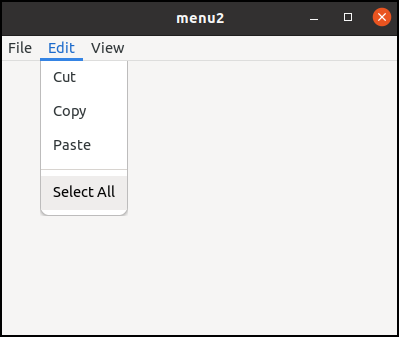
\includegraphics[width=5.985cm,height=5.055cm]{../image/menu.png}
\caption{Menu}
\end{figure}

Now let's analyze the menu above. There are two types of object.

\begin{itemize}
\tightlist
\item
  ``File'', ``Edit'', ``View'', ``Cut'', ``Copy'', ``Paste'' and
  ``Select All''. They are called ``menu item'' or simply ``item''. When
  the user clicks one of these items, then something will happen.
\item
  Menubar, submenu referenced by ``Edit'' item and two sections. They
  are called ``menu''. Menu is an ordered list of items. They are
  similar to arrays.
\end{itemize}

\begin{figure}
\centering
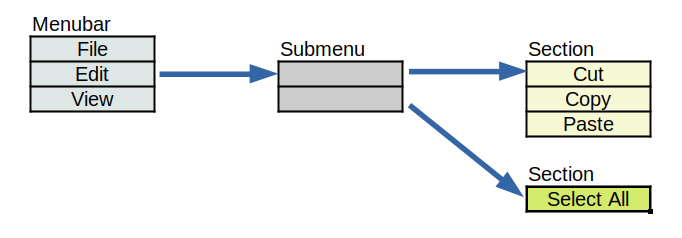
\includegraphics[width=10.23cm,height=3.57cm]{../image/menu_structure.png}
\caption{Menu structure}
\end{figure}

\begin{itemize}
\tightlist
\item
  Menubar is a menu which has three items, which are ``File'', ``Edit''
  and ``View''.
\item
  The menu item labeled ``Edit'' has a link to the submenu which has two
  items. These two items don't have labels. Each item refers to a
  section.
\item
  The first section is a menu which has three items -- ``Cut'', ``Copy''
  and ``Paste''.
\item
  The second section is a menu which has one item -- ``Select All''.
\end{itemize}

Menus can build a complicated structure thanks to the links of menu
items.

\hypertarget{gmenumodel-gmenu-and-gmenuitem}{%
\subsection{GMenuModel, GMenu and
GMenuItem}\label{gmenumodel-gmenu-and-gmenuitem}}

GMenuModel is an abstract object which represents a menu. GMenu is a
simple implementation of GMenuModel and a child object of GMenuModel.

\begin{lstlisting}
GObject -- GMenuModel -- GMenu
\end{lstlisting}

Because GMenuModel is an abstract object, it isn't instantiatable.
Therefore, it doesn't have any functions to create its instance. If you
want to create a menu, use \passthrough{\lstinline!g\_menu\_new!} to
create a GMenu instance. GMenu inherits all the functions of GMenuModel
because of the child object.

GMenuItem is an object directly derived from GObject. GMenuItem and
Gmenu (or GMenuModel) don't have a parent-child relationship.

\begin{lstlisting}
GObject -- GMenuModel -- GMenu
GObject -- GMenuItem
\end{lstlisting}

GMenuItem has attributes. One of the attributes is label. For example,
there is a menu item which has ``Edit'' label in the first diagram in
this section. ``Cut'', ``Copy'', ``Paste'' and ``Select All'' are also
the labels of the menu items. Other attributes will be explained later.

Some menu items have a link to another GMenu. There are two types of
links, submenu and section.

GMenuItem can be inserted, appended or prepended to GMenu. When it is
inserted, all of the attributes and link values of the item are copied
and used to form a new item within the menu. The GMenuItem itself is not
really inserted. Therefore, after the insertion, GMenuItem is useless
and it should be freed. The same goes for appending or prepending.

The following code shows how to append GMenuItem to GMenu.

\begin{lstlisting}
GMenu *menu = g_menu_new ();
GMenuItem *menu_item_quit = g_menu_item_new ("Quit", "app.quit");
g_menu_append_item (menu, menu_item_quit);
g_object_unref (menu_item_quit);
\end{lstlisting}

\hypertarget{menu-and-action-1}{%
\subsection{Menu and action}\label{menu-and-action-1}}

One of the attributes of menu items is an action. This attribute points
an action object.

There are two action objects, GSimpleAction and GPropertyAction.
GSimpleAction is often used. And it is used with a menu item. Only
GSimpleAction is described in this section.

An action corresponds to a menu item will be activated when the menu
item is clicked. Then the action emits an activate signal.

\begin{enumerate}
\def\labelenumi{\arabic{enumi}.}
\tightlist
\item
  menu item is clicked.
\item
  The corresponding action is activated.
\item
  The action emits a signal.
\item
  The connected handler is invoked.
\end{enumerate}

The following code is an example.

\begin{lstlisting}[language=C]
static void
quit_activated(GSimpleAction *action, GVariant *parameter, gpointer app) { ... ... ...}

GSimpleAction *act_quit = g_simple_action_new ("quit", NULL);
g_action_map_add_action (G_ACTION_MAP (app), G_ACTION (act_quit));
g_signal_connect (act_quit, "activate", G_CALLBACK (quit_activated), app);
GMenuItem *menu_item_quit = g_menu_item_new ("Quit", "app.quit");
\end{lstlisting}

\begin{enumerate}
\def\labelenumi{\arabic{enumi}.}
\tightlist
\item
  \passthrough{\lstinline!menu\_item\_quit!} is a menu item. It has a
  label ``Quit'' and is connected to an action ``app.quit''. ``app'' is
  a prefix and ``quit'' is a name of the action. The prefix ``app''
  means that the action belongs to a GtkApplication instance. If the
  menu is clicked, then the corresponding action ``quit'' which belongs
  to the GtkApplication will be activated.
\item
  \passthrough{\lstinline!act\_quit!} is an action. It has a name
  ``quit''. The function
  \passthrough{\lstinline!g\_simple\_action\_new!} creates a stateless
  action. So, \passthrough{\lstinline!act\_quit!} is stateless. The
  meaning of stateless will be explained later. The argument
  \passthrough{\lstinline!NULL!} means that the action doesn't have an
  parameter. Most of the actions are stateless and have no parameter.
\item
  The action \passthrough{\lstinline!act\_quit!} is added to the
  GtkApplication instance with
  \passthrough{\lstinline!g\_action\_map\_add\_action!}. When
  \passthrough{\lstinline!act\_quit!} is activated, it will emit
  ``activate'' signal.
\item
  ``activate'' signal of the action is connected to the handler
  \passthrough{\lstinline!quit\_activated!}. So, if the action is
  activated, the handler will be invoked.
\end{enumerate}

\hypertarget{simple-example}{%
\subsection{Simple example}\label{simple-example}}

The following is a simple example of menus and actions.

\begin{lstlisting}[language=C, numbers=left]
#include <gtk/gtk.h>

static void
quit_activated(GSimpleAction *action, GVariant *parameter, gpointer user_data) {
  GApplication *app = G_APPLICATION (user_data);

  g_application_quit (app);
}

static void
app_activate (GApplication *app, gpointer user_data) {
  GtkWidget *win = gtk_application_window_new (GTK_APPLICATION (app));
  gtk_window_set_title (GTK_WINDOW (win), "menu1");
  gtk_window_set_default_size (GTK_WINDOW (win), 400, 300);

  GSimpleAction *act_quit = g_simple_action_new ("quit", NULL);
  g_action_map_add_action (G_ACTION_MAP (app), G_ACTION (act_quit));
  g_signal_connect (act_quit, "activate", G_CALLBACK (quit_activated), app);

  GMenu *menubar = g_menu_new ();
  GMenuItem *menu_item_menu = g_menu_item_new ("Menu", NULL);
  GMenu *menu = g_menu_new ();
  GMenuItem *menu_item_quit = g_menu_item_new ("Quit", "app.quit");
  g_menu_append_item (menu, menu_item_quit);
  g_object_unref (menu_item_quit);
  g_menu_item_set_submenu (menu_item_menu, G_MENU_MODEL (menu));
  g_menu_append_item (menubar, menu_item_menu);
  g_object_unref (menu_item_menu);

  gtk_application_set_menubar (GTK_APPLICATION (app), G_MENU_MODEL (menubar));
  gtk_application_window_set_show_menubar (GTK_APPLICATION_WINDOW (win), TRUE);
  gtk_window_present (GTK_WINDOW (win));
/*  gtk_widget_show (win); is also OKay instead of gtk_window_present. */
}

#define APPLICATION_ID "com.github.ToshioCP.menu1"

int
main (int argc, char **argv) {
  GtkApplication *app;
  int stat;

  app = gtk_application_new (APPLICATION_ID, G_APPLICATION_FLAGS_NONE);
  g_signal_connect (app, "activate", G_CALLBACK (app_activate), NULL);

  stat =g_application_run (G_APPLICATION (app), argc, argv);
  g_object_unref (app);
  return stat;
}
\end{lstlisting}

\begin{itemize}
\tightlist
\item
  3-8: \passthrough{\lstinline!quit\_activated!} is a handler of the
  ``activate'' signal on the action \passthrough{\lstinline!act\_quit!}.
  Handlers of the ``activate'' signal have three parameters.

  \begin{enumerate}
  \def\labelenumi{\arabic{enumi}.}
  \tightlist
  \item
    The action instance on which the signal is emitted.
  \item
    Parameter. In this example it is \passthrough{\lstinline!NULL!}
    because the second argument of
    \passthrough{\lstinline!g\_simple\_action\_new!} (line 15) is
    \passthrough{\lstinline!NULL!}. You don' t need to care about it.
  \item
    User data. It is the fourth parameter in the
    \passthrough{\lstinline!g\_signal\_connect!} (line 18) that connects
    the action and the handler.
  \end{enumerate}
\item
  7: A function \passthrough{\lstinline!g\_application\_quit!}
  immediately quits the application.
\item
  10-34: \passthrough{\lstinline!app\_activate!} is a handler of
  ``activate'' signal on the GtkApplication instance.
\item
  12-14: Creates a GtkApplicationWindow \passthrough{\lstinline!win!}.
  And sets the title and the default size.
\item
  16: Creates GSimpleAction \passthrough{\lstinline!act\_quit!}. It is
  stateless. The first argument of
  \passthrough{\lstinline!g\_simple\_action\_new!} is a name of the
  action and the second argument is a parameter. If you don't need the
  parameter, pass \passthrough{\lstinline!NULL!}. Therefore,
  \passthrough{\lstinline!act\_quit!} has a name ``quit'' and no
  parameter.
\item
  17: Adds the action to GtkApplication \passthrough{\lstinline!app!}.
  GtkApplication implements an interface GActionMap and GActionGroup.
  GtkApplication (GActionMap) can have a group of actions and the
  actions are added with the function
  \passthrough{\lstinline!g\_action\_map\_add\_action!}. This function
  is described in
  \href{https://docs.gtk.org/gio/method.ActionMap.add_action.html}{Gio
  API Reference, g\_action\_map\_add\_action}.
\item
  18: Connects ``activate'' signal of the action and the handler
  \passthrough{\lstinline!quit\_activated!}.
\item
  20-23: Creates GMenu and GMenuItem instances.
  \passthrough{\lstinline!menubar!} and \passthrough{\lstinline!menu!}
  are GMenu. \passthrough{\lstinline!menu\_item\_menu!} and
  \passthrough{\lstinline!menu\_item\_quit!} are GMenuItem.
  \passthrough{\lstinline!menu\_item\_menu!} has a label ``Menu'' and no
  action. \passthrough{\lstinline!menu\_item\_quit!} has a label
  ``Quit'' and an action ``app.quit''. The action ``app.quit'' is a
  combination of ``app'' and ``quit''. ``app'' is a prefix and it means
  that the action belongs to GtkApplication. ``quit'' is the name of the
  action. Therefore, ``app.quit'' points the action which belongs to the
  GtkApplication instance and is named ``quit''.
\item
  24-25: Appends \passthrough{\lstinline!menu\_item\_quit!} to
  \passthrough{\lstinline!menu!}. As I mentioned before, all the
  attributes and links are copied and used to form a new item in
  \passthrough{\lstinline!menu!}. Therefore after the appending,
  \passthrough{\lstinline!menu\_item\_quit!} is no longer needed. It is
  freed by \passthrough{\lstinline!g\_object\_unref!}.
\item
  26: Sets the submenu link in
  \passthrough{\lstinline!menu\_item\_menu!} to point
  \passthrough{\lstinline!menu!}.
\item
  27-28: Appends \passthrough{\lstinline!menu\_item\_menu!} to
  \passthrough{\lstinline!menubar!}. Then frees
  \passthrough{\lstinline!menu\_item\_menu!}. GMenu and GMenuItem are
  connected and finally a menu is made up. The structure of the menu is
  shown in the diagram below.
\item
  30: The menu is inserted to GtkApplication.
\item
  31: Sets GtkApplicationWindow to show the menubar.
\item
  32: Shows the window.
\end{itemize}

\begin{figure}
\centering
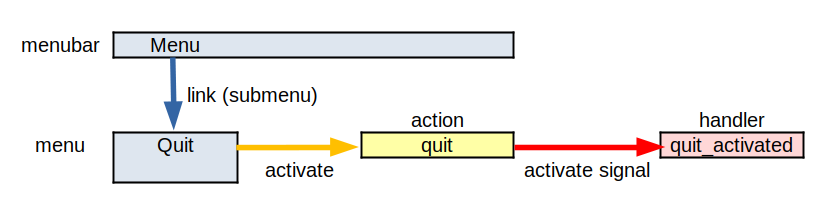
\includegraphics[width=12.555cm,height=3.285cm]{../image/menu1.png}
\caption{menu and action}
\end{figure}

\begin{figure}
\centering
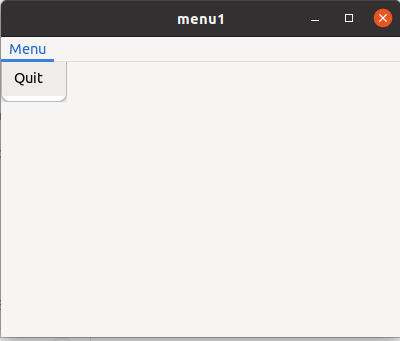
\includegraphics[width=6cm,height=5.115cm]{../image/menu1_screenshot.png}
\caption{Screenshot of menu1}
\end{figure}

  \hypertarget{stateful-action}{%
\section{Stateful action}\label{stateful-action}}

Some actions have states. The typical values of states is boolean or
string. However, other types of states are possible if you want.

There's an example \passthrough{\lstinline!menu2\_int16.c!} in the
\passthrough{\lstinline!src/men!} directory. It behaves the same as
\passthrough{\lstinline!menu2.c!}. But it uses gint16 type of states
instead of string type.

Actions which have states are called stateful.

\hypertarget{stateful-action-without-a-parameter}{%
\subsection{Stateful action without a
parameter}\label{stateful-action-without-a-parameter}}

Some menus are called toggle menu. For example, fullscreen menu has a
state which has two values -- fullscreen and non-fullscreen. The value
of the state is changed every time the menu is clicked. An action
corresponds to the fullscreen menu also have a state. Its value is TRUE
or FALSE and it is called boolean value. TRUE corresponds to fullscreen
and FALSE to non-fullscreen.

The following is an example code to implement a fullscreen menu except
the signal handler. The signal handler will be described after the
explanation of this code.

\begin{lstlisting}[language=C]
static void
app_activate (GApplication *app, gpointer user_data) {
  ... ... ...
  GSimpleAction *act_fullscreen = g_simple_action_new_stateful ("fullscreen",
                                  NULL, g_variant_new_boolean (FALSE));
  GMenuItem *menu_item_fullscreen = g_menu_item_new ("Full Screen", "win.fullscreen");
  g_signal_connect (act_fullscreen, "change-state", G_CALLBACK (fullscreen_changed), win);
  ... ... ...
}
\end{lstlisting}

\begin{itemize}
\tightlist
\item
  \passthrough{\lstinline!act\_fullscreen!} is a GSimpleAction instance.
  It is created with
  \passthrough{\lstinline!g\_simple\_action\_new\_stateful!}. The
  function has three arguments. The first argument ``fullscreen'' is the
  name of the action. The second argument is a parameter type.
  \passthrough{\lstinline!NULL!} means the action doesn't have a
  parameter. The third argument is the initial state of the action. It
  is a GVariant value. GVariant will be explained in the next
  subsection. The function
  \passthrough{\lstinline!g\_variant\_new\_boolean (FALSE)!} returns a
  GVariant value which is the boolean value
  \passthrough{\lstinline!FALSE!}.
\item
  \passthrough{\lstinline!menu\_item\_fullscreen!} is a GMenuItem
  instance. There are two arguments. The first argument ``Full Screen''
  is a label of \passthrough{\lstinline!menu\_item\_fullscreen!}. The
  second argument is an action. The action ``win.fullscreen'' has a
  prefix ``win'' and an action name ``fullscreen''. The prefix says that
  the action belongs to the window.
\item
  connects the action \passthrough{\lstinline!act\_fullscreen!} and the
  ``change-state'' signal handler
  \passthrough{\lstinline!fullscreen\_changed!}. If the fullscreen menu
  is clicked, then the corresponding action
  \passthrough{\lstinline!act\_fullscreen!} is activated. But no handler
  is connected to the ``activate'' signal. Then, the default behavior
  for boolean-stated actions with a NULL parameter type like
  \passthrough{\lstinline!act\_fullscreen!} is to toggle them via the
  ``change-state'' signal.
\end{itemize}

The following is the ``change-state'' signal handler.

\begin{lstlisting}[language=C]
static void
fullscreen_changed(GSimpleAction *action, GVariant *value, gpointer win) {
  if (g_variant_get_boolean (value))
    gtk_window_maximize (GTK_WINDOW (win));
  else
    gtk_window_unmaximize (GTK_WINDOW (win));
  g_simple_action_set_state (action, value);
}
\end{lstlisting}

\begin{itemize}
\tightlist
\item
  There are three parameters. The first parameter is the action which
  emits the ``change-state'' signal. The second parameter is the value
  of the new state of the action. The third parameter is a user data
  which is set in \passthrough{\lstinline!g\_signal\_connect!}.
\item
  If the value is boolean type and \passthrough{\lstinline!TRUE!}, then
  it maximizes the window. Otherwise unmaximizes.
\item
  Sets the state of the action with \passthrough{\lstinline!value!}.
  Note: the second argument was the toggled state value, but at this
  stage the state of the action has the original value. So, you need to
  set the state with the new value by
  \passthrough{\lstinline!g\_simple\_action\_set\_state!}.
\end{itemize}

You can use ``activate'' signal instead of ``change-state'' signal, or
both signals. But the way above is the simplest and the best.

\hypertarget{gvariant}{%
\subsubsection{GVariant}\label{gvariant}}

GVarient can contain boolean, string or other type values. For example,
the following program assigns TRUE to \passthrough{\lstinline!value!}
whose type is GVariant.

\begin{lstlisting}[language=C]
GVariant *value = g_variant_new_boolean (TRUE);
\end{lstlisting}

Another example is:

\begin{lstlisting}[language=C]
GVariant *value2 = g_variant_new_string ("Hello");
\end{lstlisting}

\passthrough{\lstinline!value2!} is a GVariant and it has a string type
value ``Hello''. GVariant can contain other types like int16, int32,
int64, double and so on.

If you want to get the original value, use g\_variant\_get series
functions. For example, you can get the boolean value by
g\_variant\_get\_boolean.

\begin{lstlisting}[language=C]
gboolean bool = g_variant_get_boolean (value);
\end{lstlisting}

Because \passthrough{\lstinline!value!} has been created as a boolean
type GVariant and \passthrough{\lstinline!TRUE!} value,
\passthrough{\lstinline!bool!} equals \passthrough{\lstinline!TRUE!}. In
the same way, you can get a string from \passthrough{\lstinline!value2!}

\begin{lstlisting}[language=C]
const char *str = g_variant_get_string (value2, NULL);
\end{lstlisting}

The second parameter is a pointer to gsize type variable (gsize is
defined as unsigned long). If it isn't NULL, then the length of the
string will be set by the function. If it is NULL, nothing happens. The
returned string \passthrough{\lstinline!str!} can't be changed.

\hypertarget{stateful-action-with-a-parameter}{%
\subsection{Stateful action with a
parameter}\label{stateful-action-with-a-parameter}}

Another example of stateful actions is an action corresponds to color
select menus. For example, there are three menus and each menu has red,
green or blue color respectively. They determine the background color of
a certain widget. One action is connected to the three menus. The action
has a state which values are ``red'', ``green'' and ``blue''. The values
are string. Those colors are given to the signal handler as a parameter.

\begin{lstlisting}[language=C]
static void
app_activate (GApplication *app, gpointer user_data) {
  ... ... ...
  GSimpleAction *act_color = g_simple_action_new_stateful ("color",
                     g_variant_type_new("s"), g_variant_new_string ("red"));
  GMenuItem *menu_item_red = g_menu_item_new ("Red", "win.color::red");
  GMenuItem *menu_item_green = g_menu_item_new ("Green", "win.color::green");
  GMenuItem *menu_item_blue = g_menu_item_new ("Blue", "win.color::blue");
  g_signal_connect (act_color, "activate", G_CALLBACK (color_activated), win);
  ... ... ...
}
\end{lstlisting}

\begin{itemize}
\tightlist
\item
  \passthrough{\lstinline!act\_color!} is a GSimpleAction instance. It
  is created with
  \passthrough{\lstinline!g\_simple\_action\_new\_stateful!}. The
  function has three arguments. The first argument ``color'' is the name
  of the action. The second argument is a parameter type which is
  GVariantType. \passthrough{\lstinline!g\_variant\_type\_new("s")!}
  creates GVariantType which is a string type
  (\passthrough{\lstinline!G\_VARIANT\_TYPE\_STRING!}). The third
  argument is the initial state of the action. It is a GVariant.
  GVariantType will be explained in the next subsection. The function
  \passthrough{\lstinline!g\_variant\_new\_string ("red")!} returns a
  GVariant value which has the string value ``red''.
\item
  \passthrough{\lstinline!menu\_item\_red!} is a GMenuItem instance.
  There are two arguments. The first argument ``Red'' is the label of
  \passthrough{\lstinline!menu\_item\_red!}. The second argument is a
  detailed action. Its prefix is ``win'', action name is ``color'' and
  target is ``red''. Target is sent to the action as a parameter. The
  same goes for \passthrough{\lstinline!menu\_item\_green!} and
  \passthrough{\lstinline!menu\_item\_blue!}.
\item
  connects the action \passthrough{\lstinline!act\_color!} and the
  ``activate'' signal handler
  \passthrough{\lstinline!color\_activated!}. If one of the three menus
  is clicked, then the action \passthrough{\lstinline!act\_color!} is
  activated with the target (parameter) which is given by the menu. No
  handler is connected to ``change-state'' signal. Then the default
  behavior is to call
  \passthrough{\lstinline!g\_simple\_action\_set\_state()!} to set the
  state to the requested value.
\end{itemize}

The following is the ``activate'' signal handler.

\begin{lstlisting}[language=C]
static void
color_activated(GSimpleAction *action, GVariant *parameter, gpointer win) {
  char *color = g_strdup_printf ("label#lb {background-color: %s;}",
                                   g_variant_get_string (parameter, NULL));
  gtk_css_provider_load_from_data (provider, color, -1);
  g_free (color);
  g_action_change_state (G_ACTION (action), parameter);
}
\end{lstlisting}

\begin{itemize}
\tightlist
\item
  There are three parameters. The first parameter is the action which
  emits the ``activate'' signal. The second parameter is the parameter
  given to the action. It is a color specified by the menu. The third
  parameter is a user data which is set in
  \passthrough{\lstinline!g\_signal\_connect!}.
\item
  \passthrough{\lstinline!color!} is a CSS string created by
  \passthrough{\lstinline!g\_strdup\_printf!}. The parameter of
  \passthrough{\lstinline!g\_strdup\_printf!} is the same as printf C
  standard function. \passthrough{\lstinline!g\_variant\_get\_string!}
  gets the string contained in \passthrough{\lstinline!parameter!}. You
  mustn't change or free the string.
\item
  Sets the color of the css provider.
\item
  Frees the string \passthrough{\lstinline!color!}.
\item
  Changes the state by
  \passthrough{\lstinline!g\_action\_change\_state!}. The function just
  sets the state of the action to the parameter by
  \passthrough{\lstinline!g\_simple\_action\_set\_state!}. Therefore,
  you can use \passthrough{\lstinline!g\_simple\_action\_set\_state!}
  instead of \passthrough{\lstinline!g\_action\_change\_state!}.
\end{itemize}

Note: If you have set a ``change-state'' signal handler,
\passthrough{\lstinline!g\_action\_change\_state!} will emit
``change-state'' signal instead of calling
\passthrough{\lstinline!g\_simple\_action\_set\_state!}.

\hypertarget{gvarianttype}{%
\subsubsection{GVariantType}\label{gvarianttype}}

GVariantType gives a type of GVariant. GVariant can contain many kinds
of types. And the type often needs to be recognized at runtime.
GVariantType provides such functionality.

GVariantType is created with a string which expresses a type.

\begin{itemize}
\tightlist
\item
  ``b'' means boolean type.
\item
  ``s'' means string type.
\end{itemize}

The following program is a simple example. It finally outputs the string
``s''.

\begin{lstlisting}[language=C, numbers=left]
#include <glib.h>

int
main (int argc, char **argv) {
  GVariantType *vtype = g_variant_type_new ("s");
  const char *type_string = g_variant_type_peek_string (vtype);
  g_print ("%s\n",type_string);
}
\end{lstlisting}

\begin{itemize}
\tightlist
\item
  \passthrough{\lstinline!g\_variant\_type\_new!} creates GVariantType.
  It uses a type string ``s'' which means string.
\item
  \passthrough{\lstinline!g\_variant\_type\_peek\_string!} takes a peek
  at \passthrough{\lstinline!vtype!}. It is the string ``s'' given to
  \passthrough{\lstinline!vtype!} when it was created.
\item
  prints the string to the terminal.
\end{itemize}

\hypertarget{example-code}{%
\subsection{Example code}\label{example-code}}

The following code includes stateful actions above. This program has
menus like this:

\begin{figure}
\centering
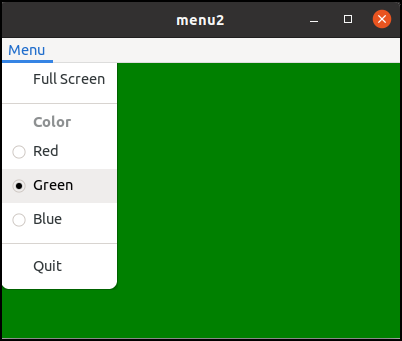
\includegraphics[width=6.03cm,height=5.115cm]{../image/menu2.png}
\caption{menu2}
\end{figure}

\begin{itemize}
\tightlist
\item
  Fullscreen menu toggles the size of the window between maximum and
  non-maximum. If the window is maximum size, which is called full
  screen, then a check mark is put before ``fullscreen'' label.
\item
  Red, green and blue menu determines the back ground color of the
  label, which is the child widget of the window. The menus have radio
  buttons on the left of the menus. And the radio button of the selected
  menu turns on.
\item
  Quit menu quits the application.
\end{itemize}

The code is as follows.

\begin{lstlisting}[language=C, numbers=left]
#include <gtk/gtk.h>

static GtkCssProvider *provider;

static void
fullscreen_changed(GSimpleAction *action, GVariant *value, gpointer win) {
  if (g_variant_get_boolean (value))
    gtk_window_maximize (GTK_WINDOW (win));
  else
    gtk_window_unmaximize (GTK_WINDOW (win));
  g_simple_action_set_state (action, value);
}

static void
color_activated(GSimpleAction *action, GVariant *parameter, gpointer win) {
  char *color = g_strdup_printf ("label#lb {background-color: %s;}", g_variant_get_string (parameter, NULL));
  gtk_css_provider_load_from_data (provider, color, -1);
  g_free (color);
  g_action_change_state (G_ACTION (action), parameter);
}

static void
quit_activated(GSimpleAction *action, GVariant *parameter, gpointer app)
{
  g_application_quit (G_APPLICATION(app));
}

static void
app_activate (GApplication *app, gpointer user_data) {
  GtkWidget *win = gtk_application_window_new (GTK_APPLICATION (app));
  gtk_window_set_title (GTK_WINDOW (win), "menu2");
  gtk_window_set_default_size (GTK_WINDOW (win), 400, 300);

  GtkWidget *lb = gtk_label_new (NULL);
  gtk_widget_set_name (lb, "lb"); /* the name is used by CSS Selector */
  gtk_window_set_child (GTK_WINDOW (win), lb);

  GSimpleAction *act_fullscreen
    = g_simple_action_new_stateful ("fullscreen", NULL, g_variant_new_boolean (FALSE));
  GSimpleAction *act_color
    = g_simple_action_new_stateful ("color", g_variant_type_new("s"), g_variant_new_string ("red"));
  GSimpleAction *act_quit
    = g_simple_action_new ("quit", NULL);

  GMenu *menubar = g_menu_new ();
  GMenu *menu = g_menu_new ();
  GMenu *section1 = g_menu_new ();
  GMenu *section2 = g_menu_new ();
  GMenu *section3 = g_menu_new ();
  GMenuItem *menu_item_fullscreen = g_menu_item_new ("Full Screen", "win.fullscreen");
  GMenuItem *menu_item_red = g_menu_item_new ("Red", "win.color::red");
  GMenuItem *menu_item_green = g_menu_item_new ("Green", "win.color::green");
  GMenuItem *menu_item_blue = g_menu_item_new ("Blue", "win.color::blue");
  GMenuItem *menu_item_quit = g_menu_item_new ("Quit", "app.quit");

  g_signal_connect (act_fullscreen, "change-state", G_CALLBACK (fullscreen_changed), win);
  g_signal_connect (act_color, "activate", G_CALLBACK (color_activated), win);
  g_signal_connect (act_quit, "activate", G_CALLBACK (quit_activated), app);
  g_action_map_add_action (G_ACTION_MAP (win), G_ACTION (act_fullscreen));
  g_action_map_add_action (G_ACTION_MAP (win), G_ACTION (act_color));
  g_action_map_add_action (G_ACTION_MAP (app), G_ACTION (act_quit));

  g_menu_append_item (section1, menu_item_fullscreen);
  g_menu_append_item (section2, menu_item_red);
  g_menu_append_item (section2, menu_item_green);
  g_menu_append_item (section2, menu_item_blue);
  g_menu_append_item (section3, menu_item_quit);
  g_object_unref (menu_item_red);
  g_object_unref (menu_item_green);
  g_object_unref (menu_item_blue);
  g_object_unref (menu_item_fullscreen);
  g_object_unref (menu_item_quit);

  g_menu_append_section (menu, NULL, G_MENU_MODEL (section1));
  g_menu_append_section (menu, "Color", G_MENU_MODEL (section2));
  g_menu_append_section (menu, NULL, G_MENU_MODEL (section3));
  g_menu_append_submenu (menubar, "Menu", G_MENU_MODEL (menu));

  gtk_application_set_menubar (GTK_APPLICATION (app), G_MENU_MODEL (menubar));
  gtk_application_window_set_show_menubar (GTK_APPLICATION_WINDOW (win), TRUE);

/*  GtkCssProvider *provider = gtk_css_provider_new ();*/
  provider = gtk_css_provider_new ();
  GdkDisplay *display = gtk_widget_get_display (GTK_WIDGET (win));
  gtk_css_provider_load_from_data (provider, "label#lb {background-color: red;}", -1);
  gtk_style_context_add_provider_for_display (display, GTK_STYLE_PROVIDER (provider),
                                              GTK_STYLE_PROVIDER_PRIORITY_USER);

/*  gtk_widget_show (win);*/
  gtk_window_present (GTK_WINDOW (win));
}

#define APPLICATION_ID "com.github.ToshioCP.menu2"

int
main (int argc, char **argv) {
  GtkApplication *app;
  int stat;

  app = gtk_application_new (APPLICATION_ID, G_APPLICATION_FLAGS_NONE);
  g_signal_connect (app, "activate", G_CALLBACK (app_activate), NULL);

  stat =g_application_run (G_APPLICATION (app), argc, argv);
  g_object_unref (app);
  return stat;
}
\end{lstlisting}

\begin{itemize}
\tightlist
\item
  5-26: Signal handlers. They have already been explained.
\item
  30-36: \passthrough{\lstinline!win!} and \passthrough{\lstinline!lb!}
  are GtkApplicationWindow and GtkLabel respectively.
  \passthrough{\lstinline!win!} has a title ``menu2'' and its default
  size is 400x300. \passthrough{\lstinline!lb!} is named as ``lb''. The
  name is used in CSS. \passthrough{\lstinline!lb!} is set to
  \passthrough{\lstinline!win!} as a child.
\item
  38-43: Three actions are defined. They are:

  \begin{itemize}
  \tightlist
  \item
    stateful and has no parameter. It has a toggle state.
  \item
    stateful and has a parameter. Parameter is a string type.
  \item
    stateless and has no parameter.
  \end{itemize}
\item
  45-54: Creates GMenu and GMenuItem. There are three sections.
\item
  56-61: Signals are connected to handlers. And actions are added to
  GActionMap. Because \passthrough{\lstinline!act\_fullscreen!} and
  \passthrough{\lstinline!act\_color!} have ``win'' prefix and belong to
  GtkApplicationWindow, they are added to \passthrough{\lstinline!win!}.
  GtkApplicationWindow implements GActionModel interface like
  GtkApplication. \passthrough{\lstinline!act\_quit!} has ``app'' prefix
  and belongs to GtkApplication. It is added to
  \passthrough{\lstinline!app!}.
\item
  63-77: Connects and builds the menus. Useless GMenuItem are freed.
\item
  79-80: GMenuModel \passthrough{\lstinline!menubar!} is inserted to
  \passthrough{\lstinline!app!}. Sets show menubar property of
  \passthrough{\lstinline!win!} to \passthrough{\lstinline!TRUE!}. Note:
  \passthrough{\lstinline!gtk\_application\_window\_set\_show\_menubar!}
  creates GtkPopoverMenubar from GMenuModel. This is a different point
  between Gtk3 and Gtk4. And you can use GtkPopoverMenubar directly and
  set it as a descendant widget of the window. You may use GtkBox as a
  child widget of the window and insert GtkPopoverMenubar as the first
  child of the box.
\item
  82-87: Sets CSS. \passthrough{\lstinline!provider!} is GtkCssProvider
  which is defined in line three as a static variable. Its CSS data is:
  \passthrough{\lstinline!label\#lb \{background-color: red;\}!}.
  ``label\#lb'' is called selector. ``label'' is the node of GtkLabel.
  ``\#'' precedes an ID which is an identifiable name of the widget.
  ``lb'' is the name of GtkLabel \passthrough{\lstinline!lb!}. (See line
  35). The style is surrounded by open and close braces. The style is
  applied to GtkLabel which has a name ``lb''. Other GtkLabel have no
  effect from this. The provider is added to GdkDisplay.
\item
  90: Shows the window.
\end{itemize}

  \hypertarget{ui-file-for-menu-and-action-entries}{%
\section{Ui file for menu and action
entries}\label{ui-file-for-menu-and-action-entries}}

\hypertarget{ui-file-for-menu}{%
\subsection{Ui file for menu}\label{ui-file-for-menu}}

You might have thought that building menus is really bothersome. Yes,
the program was complicated and it needs lots of time to code it. The
situation is similar to building widgets. When we built widgets, using
ui file was a good way to avoid such complicated coding. The same goes
for menus.

The ui file for menus has interface, menu tags. The file starts and ends
with interface tag.

\begin{lstlisting}[language=XML]
<interface>
  <menu id="menubar">
  </menu>
</interface>
\end{lstlisting}

\passthrough{\lstinline!menu!} tag corresponds to GMenu object.
\passthrough{\lstinline!id!} attribute defines the name of the object.
It will be referred by GtkBuilder.

\begin{lstlisting}[language=XML]
<submenu>
  <attribute name="label">File</attribute>
    <item>
      <attribute name="label">New</attribute>
      <attribute name="action">win.new</attribute>
    </item>
</submenu>
\end{lstlisting}

\passthrough{\lstinline!item!} tag corresponds to item in GMenu which
has the same structure as GMenuItem. The item above has a label
attribute. Its value is ``New''. The item also has an action attribute
and its value is ``win.new''. ``win'' is a prefix and ``new'' is an
action name. \passthrough{\lstinline!submenu!} tag corresponds to both
GMenuItem and GMenu. The GMenuItem has a link to GMenu.

The ui file above can be described as follows.

\begin{lstlisting}[language=XML]
<item>
  <attribute name="label">File</attribute>
    <link name="submenu">
      <item>
        <attribute name="label">New</attribute>
        <attribute name="action">win.new</attribute>
      </item>
    </link>
</item>
\end{lstlisting}

\passthrough{\lstinline!link!} tag expresses the link to submenu. And at
the same time it also expresses the submenu itself. This file
illustrates the relationship between the menus and items better than the
prior ui file. But \passthrough{\lstinline!submenu!} tag is simple and
easy to understand. So, we usually prefer the former ui file style.

The following is a screenshot of the sample program in this section. Its
name is \passthrough{\lstinline!menu3!}.

\begin{figure}
\centering
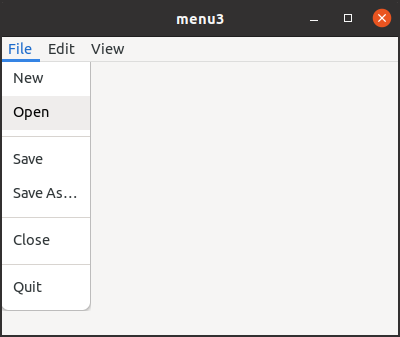
\includegraphics[width=6cm,height=5.055cm]{../image/menu3.png}
\caption{menu3}
\end{figure}

The following is the ui file of the menu in
\passthrough{\lstinline!menu3!}.

\begin{lstlisting}[language=XML, numbers=left]
<?xml version="1.0" encoding="UTF-8"?>
<interface>
  <menu id="menubar">
    <submenu>
      <attribute name="label">File</attribute>
      <section>
        <item>
          <attribute name="label">New</attribute>
          <attribute name="action">win.new</attribute>
        </item>
        <item>
          <attribute name="label">Open</attribute>
          <attribute name="action">win.open</attribute>
        </item>
      </section>
      <section>
        <item>
          <attribute name="label">Save</attribute>
          <attribute name="action">win.save</attribute>
        </item>
        <item>
          <attribute name="label">Save As…</attribute>
          <attribute name="action">win.saveas</attribute>
        </item>
      </section>
      <section>
        <item>
          <attribute name="label">Close</attribute>
          <attribute name="action">win.close</attribute>
        </item>
      </section>
      <section>
        <item>
          <attribute name="label">Quit</attribute>
          <attribute name="action">app.quit</attribute>
        </item>
      </section>
    </submenu>
    <submenu>
      <attribute name="label">Edit</attribute>
      <section>
        <item>
          <attribute name="label">Cut</attribute>
          <attribute name="action">win.cut</attribute>
        </item>
        <item>
          <attribute name="label">Copy</attribute>
          <attribute name="action">win.copy</attribute>
        </item>
        <item>
          <attribute name="label">Paste</attribute>
          <attribute name="action">win.paste</attribute>
        </item>
      </section>
      <section>
        <item>
          <attribute name="label">Select All</attribute>
          <attribute name="action">win.selectall</attribute>
        </item>
      </section>
    </submenu>
    <submenu>
      <attribute name="label">View</attribute>
      <section>
        <item>
          <attribute name="label">Full Screen</attribute>
          <attribute name="action">win.fullscreen</attribute>
        </item>
      </section>
    </submenu>
  </menu>
</interface>
\end{lstlisting}

The ui file is converted to the resource by the resource compiler
\passthrough{\lstinline!glib-compile-resouces!} with xml file below.

\begin{lstlisting}[language=XML, numbers=left]
<?xml version="1.0" encoding="UTF-8"?>
<gresources>
  <gresource prefix="/com/github/ToshioCP/menu3">
    <file>menu3.ui</file>
  </gresource>
</gresources>
\end{lstlisting}

GtkBuilder builds menus from the resource.

\begin{lstlisting}[language=C]
GtkBuilder *builder = gtk_builder_new_from_resource ("/com/github/ToshioCP/menu3/menu3.ui");
GMenuModel *menubar = G_MENU_MODEL (gtk_builder_get_object (builder, "menubar"));

gtk_application_set_menubar (GTK_APPLICATION (app), menubar);
g_object_unref (builder);
\end{lstlisting}

It is important that \passthrough{\lstinline!builder!} is unreferred
after the GMenuModel \passthrough{\lstinline!menubar!} is inserted to
the application. If you do it before setting, bad thing will happen --
your computer might freeze.

\hypertarget{action-entry}{%
\subsection{Action entry}\label{action-entry}}

The coding for building actions and signal handlers is bothersome work
as well. Therefore, it should be automated. You can implement them
easily with GActionEntry structure and
\passthrough{\lstinline!g\_action\_map\_add\_action\_entries!} function.

GActionEntry contains action name, signal handlers, parameter and state.

\begin{lstlisting}[language=C]
typedef struct _GActionEntry GActionEntry;

struct _GActionEntry
{
  /* action name */
  const gchar *name;
  /* activate handler */
  void (* activate) (GSimpleAction *action, GVariant *parameter, gpointer user_data);
  /* the type of the parameter given as a single GVariant type string */
  const gchar *parameter_type;
  /* initial state given in GVariant text format */
  const gchar *state;
  /* change-state handler */
  void (* change_state) (GSimpleAction *action, GVariant *value, gpointer user_data);
  /*< private >*/
  gsize padding[3];
};
\end{lstlisting}

For example, the actions in the previous section are:

\begin{lstlisting}[language=C]
{ "fullscreen", NULL, NULL, "false", fullscreen_changed }
{ "color", color_activated, "s", "red", NULL }
{ "quit", quit_activated, NULL, NULL, NULL },
\end{lstlisting}

And \passthrough{\lstinline!g\_action\_map\_add\_action\_entries!} does
all the process instead of the functions you have needed.

\begin{lstlisting}[language=C]
const GActionEntry app_entries[] = {
  { "quit", quit_activated, NULL, NULL, NULL }
};
g_action_map_add_action_entries (G_ACTION_MAP (app), app_entries,
                                 G_N_ELEMENTS (app_entries), app);
\end{lstlisting}

The code above does:

\begin{itemize}
\tightlist
\item
  Builds the ``quit'' action
\item
  Connects the action and the ``activate'' signal handler
  \passthrough{\lstinline!quit\_activated!}
\item
  Adds the action to the action map \passthrough{\lstinline!app!}.
\end{itemize}

The same goes for the other actions.

\begin{lstlisting}[language=C]
const GActionEntry win_entries[] = {
  { "fullscreen", NULL, NULL, "false", fullscreen_changed },
  { "color", color_activated, "s", "red", NULL }
};
g_action_map_add_action_entries (G_ACTION_MAP (win), win_entries,
                                 G_N_ELEMENTS (win_entries), win);
\end{lstlisting}

The code above does:

\begin{itemize}
\tightlist
\item
  Builds a ``fullscreen'' action and ``color'' action.
\item
  Connects the ``fullscreen'' action and the ``change-state'' signal
  handler \passthrough{\lstinline!fullscreen\_changed!}
\item
  Its initial state is set to FALSE.
\item
  Connects the ``color'' action and the ``activate'' signal handler
  \passthrough{\lstinline!color\_activated!}
\item
  Its parameter type is string and the initial value is ``red''.
\item
  Adds the actions to the action map \passthrough{\lstinline!win!}.
\end{itemize}

\hypertarget{example-code}{%
\subsection{Example code}\label{example-code}}

The C source code of \passthrough{\lstinline!menu3!} and
\passthrough{\lstinline!meson.build!} is as follows.

\begin{lstlisting}[language=C, numbers=left]
#include <gtk/gtk.h>

static void
new_activated (GSimpleAction *action, GVariant *parameter, gpointer win) {
}

static void
open_activated (GSimpleAction *action, GVariant *parameter, gpointer win) {
}

static void
save_activated (GSimpleAction *action, GVariant *parameter, gpointer win) {
}

static void
saveas_activated (GSimpleAction *action, GVariant *parameter, gpointer win) {
}

static void
close_activated (GSimpleAction *action, GVariant *parameter, gpointer win) {
}

static void
cut_activated (GSimpleAction *action, GVariant *parameter, gpointer win) {
}

static void
copy_activated (GSimpleAction *action, GVariant *parameter, gpointer win) {
}

static void
paste_activated (GSimpleAction *action, GVariant *parameter, gpointer win) {
}

static void
selectall_activated (GSimpleAction *action, GVariant *parameter, gpointer win) {
}

static void
fullscreen_changed (GSimpleAction *action, GVariant *state, gpointer win) {
  if (g_variant_get_boolean (state))
    gtk_window_maximize (GTK_WINDOW (win));
  else
    gtk_window_unmaximize (GTK_WINDOW (win));
  g_simple_action_set_state (action, state);
}

static void
quit_activated (GSimpleAction *action, GVariant *parameter, gpointer app)
{
  g_application_quit (G_APPLICATION(app));
}

static void
app_activate (GApplication *app, gpointer user_data) {
  GtkWidget *win = gtk_application_window_new (GTK_APPLICATION (app));

  const GActionEntry win_entries[] = {
    { "new", new_activated, NULL, NULL, NULL },
    { "open", open_activated, NULL, NULL, NULL },
    { "save", save_activated, NULL, NULL, NULL },
    { "saveas", saveas_activated, NULL, NULL, NULL },
    { "close", close_activated, NULL, NULL, NULL },
    { "cut", cut_activated, NULL, NULL, NULL },
    { "copy", copy_activated, NULL, NULL, NULL },
    { "paste", paste_activated, NULL, NULL, NULL },
    { "selectall", selectall_activated, NULL, NULL, NULL },
    { "fullscreen", NULL, NULL, "false", fullscreen_changed }
  };
  g_action_map_add_action_entries (G_ACTION_MAP (win), win_entries, G_N_ELEMENTS (win_entries), win);

  gtk_application_window_set_show_menubar (GTK_APPLICATION_WINDOW (win), TRUE);

  gtk_window_set_title (GTK_WINDOW (win), "menu3");
  gtk_window_set_default_size (GTK_WINDOW (win), 400, 300);
  gtk_widget_show (win);
}

static void
app_startup (GApplication *app, gpointer user_data) {
  GtkBuilder *builder = gtk_builder_new_from_resource ("/com/github/ToshioCP/menu3/menu3.ui");
  GMenuModel *menubar = G_MENU_MODEL (gtk_builder_get_object (builder, "menubar"));

  gtk_application_set_menubar (GTK_APPLICATION (app), menubar);
  g_object_unref (builder);

  const GActionEntry app_entries[] = {
    { "quit", quit_activated, NULL, NULL, NULL }
  };
  g_action_map_add_action_entries (G_ACTION_MAP (app), app_entries, G_N_ELEMENTS (app_entries), app);
}

#define APPLICATION_ID "com.github.ToshioCP.menu3"

int
main (int argc, char **argv) {
  GtkApplication *app;
  int stat;

  app = gtk_application_new (APPLICATION_ID, G_APPLICATION_FLAGS_NONE);
  g_signal_connect (app, "startup", G_CALLBACK (app_startup), NULL);
  g_signal_connect (app, "activate", G_CALLBACK (app_activate), NULL);

  stat =g_application_run (G_APPLICATION (app), argc, argv);
  g_object_unref (app);
  return stat;
}
\end{lstlisting}

meson.build

\begin{lstlisting}[numbers=left]
project('menu3', 'c')

gtkdep = dependency('gtk4')

gnome=import('gnome')
resources = gnome.compile_resources('resources','menu3.gresource.xml')

sourcefiles=files('menu3.c')

executable('menu3', sourcefiles, resources, dependencies: gtkdep)
\end{lstlisting}

  \hypertarget{gtkmenubutton-accelerators-font-pango-and-gsettings}{%
\section{GtkMenuButton, accelerators, font, pango and
gsettings}\label{gtkmenubutton-accelerators-font-pango-and-gsettings}}

Traditional menu structure is fine. However, buttons or menu items we
often use are not so many. Some mightn't be clicked at all. Therefore,
it's a good idea to put some frequently used buttons on the toolbar and
put the rest of the less frequently used operations into the menu. Such
menu are often connected to GtkMenuButton.

We will restructure tfe text file editor in this section. It will be
more practical. The buttons are changed to:

\begin{itemize}
\tightlist
\item
  Put open, save and close buttons to the toolbar. In addition,
  GtkMenuButton is added to the toolbar. This button shows a popup menu
  when clicked on. Here, popup means widely, including pull-down menu.
\item
  Put new, save as, preference and quit items to the menu under the menu
  button.
\end{itemize}

\hypertarget{signal-elements-in-ui-files}{%
\subsection{Signal elements in ui
files}\label{signal-elements-in-ui-files}}

The four buttons are included in the ui file
\passthrough{\lstinline!tfe.ui!}. The difference from prior sections is
signal tag. The following is extracted from
\passthrough{\lstinline!tfe.ui!} and it describes the open button.

\begin{lstlisting}[language=XML]
<object class="GtkButton" id="btno">
  <property name="label">Open</property>
  <signal name="clicked" handler="open_cb" swapped="TRUE" object="nb"></signal>
</object>
\end{lstlisting}

Signal tag specifies the name of the signal, handler and user\_data
object. They are the value of name, handler and object attributes.
Swapped attribute has the same meaning as
\passthrough{\lstinline!g\_signal\_connect\_swapped!} function. So, the
signal tag above works the same as the function below.

\begin{lstlisting}[language=C]
g_signal_connect_swapped (btno, "clicked", G_CALLBACK (open_cb), nb);
\end{lstlisting}

You need to compile the source file with ``-WI, --export-dynamic''
options. You can achieve this by adding ``export\_dynamic: true''
argument to executable function in
\passthrough{\lstinline!meson.build!}. And remove static class from the
handler.

\begin{lstlisting}[language=C]
void
open_cb (GtkNotebook *nb) {
  notebook_page_open (nb);
}
\end{lstlisting}

If you add static, the function is in the scope of the file and it can't
be seen from outside. Then the signal tag can't find the function.

\hypertarget{menu-and-gkmenubutton}{%
\subsection{Menu and GkMenuButton}\label{menu-and-gkmenubutton}}

Menus are described in \passthrough{\lstinline!menu.ui!} file.

\begin{lstlisting}[language=XML, numbers=left]
<?xml version="1.0" encoding="UTF-8"?>
<interface>
  <menu id="menu">
    <section>
      <item>
        <attribute name="label">New</attribute>
        <attribute name="action">win.new</attribute>
      </item>
      <item>
        <attribute name="label">Save As…</attribute>
        <attribute name="action">win.saveas</attribute>
      </item>
    </section>
    <section>
      <item>
        <attribute name="label">Preference</attribute>
        <attribute name="action">win.pref</attribute>
      </item>
    </section>
    <section>
      <item>
        <attribute name="label">Quit</attribute>
        <attribute name="action">win.close-all</attribute>
      </item>
    </section>
  </menu>
</interface>
\end{lstlisting}

There are four items, ``New'', ``Saveas'', ``Preference'' and ``Quit''.

\begin{itemize}
\tightlist
\item
  ``New'' menu creates a new empty page.
\item
  ``Saveas'' menu saves the current page as a new filename.
\item
  ``Preference'' menu sets preference items. This version of
  \passthrough{\lstinline!tfe!} has only font preference.
\item
  ``Quit'' menu quits the application.
\end{itemize}

These four menus are not used so often. That's why they are put to the
menu behind the menu button.

The menus and the menu button are connected with
\passthrough{\lstinline!gtk\_menu\_button\_set\_menu\_model!} function.
The variable \passthrough{\lstinline!btnm!} below points a GtkMenuButton
object.

\begin{lstlisting}[language=C]
  build = gtk_builder_new_from_resource ("/com/github/ToshioCP/tfe/menu.ui");
  menu = G_MENU_MODEL (gtk_builder_get_object (build, "menu"));
  gtk_menu_button_set_menu_model (btnm, menu);
\end{lstlisting}

\hypertarget{actions-and-accelerators}{%
\subsection{Actions and Accelerators}\label{actions-and-accelerators}}

Menus are connected to actions. Actions are defined with an array and
\passthrough{\lstinline!g\_action\_map\_add\_action\_entries!} function.

\begin{lstlisting}[language=C]
  const GActionEntry win_entries[] = {
    { "open", open_activated, NULL, NULL, NULL },
    { "save", save_activated, NULL, NULL, NULL },
    { "close", close_activated, NULL, NULL, NULL },
    { "new", new_activated, NULL, NULL, NULL },
    { "saveas", saveas_activated, NULL, NULL, NULL },
    { "pref", pref_activated, NULL, NULL, NULL },
    { "close-all", quit_activated, NULL, NULL, NULL }
  };
  g_action_map_add_action_entries (G_ACTION_MAP (win), win_entries, G_N_ELEMENTS (win_entries), nb);
\end{lstlisting}

There are seven actions, open, save, close, new, saveas, pref and
close-all. But there were only four menus. New, saveas, pref and
close-all actions correspond to new, saveas, preference and quit menu
respectively. The three actions open, save and close doesn't have
corresponding menus. Are thy necessary? These actions are defined
because of accelerators.

Accelerators are a kind of short cut key function. They are defined with
arrays and
\passthrough{\lstinline!gtk\_application\_set\_accels\_for\_action!}
function.

\begin{lstlisting}[language=C]
  struct {
    const char *action;
    const char *accels[2];
  } action_accels[] = {
    { "win.open", { "<Control>o", NULL } },
    { "win.save", { "<Control>s", NULL } },
    { "win.close", { "<Control>w", NULL } },
    { "win.new", { "<Control>n", NULL } },
    { "win.saveas", { "<Shift><Control>s", NULL } },
    { "win.close-all", { "<Control>q", NULL } },
  };

  for (i = 0; i < G_N_ELEMENTS(action_accels); i++)
    gtk_application_set_accels_for_action(GTK_APPLICATION(app), action_accels[i].action, action_accels[i].accels);
\end{lstlisting}

This code is a bit complicated. The array
\passthrough{\lstinline!action-accels[]!} is an array of structures. The
structure is:

\begin{lstlisting}[language=C]
  struct {
    const char *action;
    const char *accels[2];
  }
\end{lstlisting}

The member \passthrough{\lstinline!action!} is a string. The member
\passthrough{\lstinline!accels!} is an array of two strings. For
example,

\begin{lstlisting}[language=C]
{ "win.open", { "<Control>o", NULL } },
\end{lstlisting}

This is the first element of the array
\passthrough{\lstinline!action\_accels!}.

\begin{itemize}
\tightlist
\item
  The member \passthrough{\lstinline!action!} is ``win.open''. This
  specifies the action ``open'' belongs to the window object.
\item
  The member \passthrough{\lstinline!accels!} is an array of two
  strings, ``\textless Control\textgreater o'' and NULL. The first
  string specifies a key combination. Control key and `o'. If you keep
  pressing the control key and push `o' key, then it activates the
  action \passthrough{\lstinline!win.open!}. The second string NULL (or
  zero) means the end of the list (array). You can define more than one
  accelerator keys and the list must ends with NULL (zero). If you want
  to do so, the array length needs to be three or more. The parser
  recognizes ``\textless control\textgreater o'',
  ``\textless Shift\textgreater\textless Alt\textgreater F2'',
  ``\textless Ctrl\textgreater minus'' and so on. If you want to use
  symbol key like ``\textless Ctrl\textgreater-'', use
  ``\textless Ctrl\textgreater minus'' instead. Such relation between
  lower case and symbol (its character code) is specified in
  \href{https://gitlab.gnome.org/GNOME/gtk/-/blob/master/gdk/gdkkeysyms.h}{\passthrough{\lstinline!gdkkeysyms.h!}}
  in the Gtk4 source code.
\end{itemize}

\hypertarget{saveas-handler}{%
\subsection{Saveas handler}\label{saveas-handler}}

TfeTextView has already had a saveas function. So, only we need to write
is the wrapper function in \passthrough{\lstinline!tfenotebook.c!}.

\begin{lstlisting}[language=C, numbers=left]
static TfeTextView *
get_current_textview (GtkNotebook *nb) {
  int i;
  GtkWidget *scr;
  GtkWidget *tv;

  i = gtk_notebook_get_current_page (nb);
  scr = gtk_notebook_get_nth_page (nb, i);
  tv = gtk_scrolled_window_get_child (GTK_SCROLLED_WINDOW (scr));
  return TFE_TEXT_VIEW (tv);
}

void
notebook_page_saveas (GtkNotebook *nb) {
  g_return_if_fail(GTK_IS_NOTEBOOK (nb));

  TfeTextView *tv;

  tv = get_current_textview (nb);
  tfe_text_view_saveas (TFE_TEXT_VIEW (tv));
}
\end{lstlisting}

The function \passthrough{\lstinline!get\_current\_textview!} is the
same as before. The function
\passthrough{\lstinline!notebook\_page\_saveas!} simply calls
\passthrough{\lstinline!tfe\_text\_view\_saveas!}.

In \passthrough{\lstinline!tfeapplication.c!}, saveas handler just call
\passthrough{\lstinline!notebook\_page\_saveas!}.

\begin{lstlisting}[language=C, numbers=left]
static void
saveas_activated (GSimpleAction *action, GVariant *parameter, gpointer user_data) {
  GtkNotebook *nb = GTK_NOTEBOOK (user_data);
  notebook_page_saveas (nb);
}
\end{lstlisting}

\hypertarget{preference-and-alert-dialog}{%
\subsection{Preference and alert
dialog}\label{preference-and-alert-dialog}}

\hypertarget{preference-dialog}{%
\subsubsection{Preference dialog}\label{preference-dialog}}

Preference dialog xml definition is added to
\passthrough{\lstinline!tfe.ui!}.

\begin{lstlisting}[language=XML]
<object class="GtkDialog" id="pref">
  <property name="title">Preferences</property>
  <property name="resizable">FALSE</property>
  <property name="modal">TRUE</property>
  <property name="transient-for">win</property>
  <child internal-child="content_area">
    <object class="GtkBox" id="content_area">
      <child>
        <object class="GtkBox" id="pref_boxh">
          <property name="orientation">GTK_ORIENTATION_HORIZONTAL</property>
          <property name="spacing">12</property>
          <property name="margin-start">12</property>
          <property name="margin-end">12</property>
          <property name="margin-top">12</property>
          <property name="margin-bottom">12</property>
          <child>
            <object class="GtkLabel" id="fontlabel">
              <property name="label">Font:</property>
              <property name="xalign">1</property>
            </object>
          </child>
          <child>
            <object class="GtkFontButton" id="fontbtn">
            </object>
          </child>
        </object>
      </child>
    </object>
  </child>
</object>
\end{lstlisting}

\begin{itemize}
\tightlist
\item
  Preference dialog is an independent dialog. It is not a descendant
  widget of the top-level GtkApplicationwindow
  \passthrough{\lstinline!win!}. Therefore, There's no child tag that
  surrounds the dialog object.
\item
  There are four properties of the dialog. GtkDialog is a child object
  (not child widget) of GtkWindow, so it inherits all the properties
  from GtkWindow. Title, resizable, modal and transient-for properties
  are inherited from GtkWindow. Transient-for specifies a temporary
  parent window, which the dialog's location is based on.
\item
  internal-child attribute is used in the child tag above. GtkDialog has
  a GtkBox child widget. Its id is ``content\_area'' in
  \passthrough{\lstinline!gtkdialog.ui!}, which is the ui file of
  GtkDialog. (It is in the Gtk4 source files.) This box is provided for
  users to add content widgets in it. The tag
  \passthrough{\lstinline!<child internal-child="content\_area">!} is
  put at the top of the contents. Then you need to specify an object tag
  and define its class as GtkBox and its id as content\_area. This
  object is defined in \passthrough{\lstinline!gtkdialog.ui!} but you
  need to define it again in the child tag.
\item
  In the content area, defines GtkBox, GtkLabel and GtkFontButton.
\end{itemize}

I want the preference dialog to keep alive during the application lives.
So, it is necessary to catch ``close-request'' signal from the dialog
and stop the signal propagation. This is accomplished by returning TRUE
by the signal handler.

\begin{lstlisting}[language=C]
pref_close_cb (GtkDialog *pref, gpointer user_data) {
  return TRUE;
}

g_signal_connect (GTK_DIALOG (pref), "close-request", G_CALLBACK (pref_close_cb), NULL);
\end{lstlisting}

Generally, signal emission consists of five stages.

\begin{enumerate}
\def\labelenumi{\arabic{enumi}.}
\tightlist
\item
  Default handler is invoked if the signal's flag is
  \passthrough{\lstinline!G\_SIGNAL\_RUN\_FIRST!}. Default handler is
  set when a signal is registered. It is different from user signal
  handler, simply called signal handler, connected by
  \passthrough{\lstinline!g\_signal\_connect!}series function. Default
  handler can be invoked in either stage 1, 3 or 5. Most of the default
  handlers are \passthrough{\lstinline!G\_SIGNAL\_RUN\_FIRST!} or
  \passthrough{\lstinline!G\_SIGNAL\_RUN\_LAST!}.
\item
  Signal handlers are invoked, unless it is connected by
  \passthrough{\lstinline!g\_signal\_connect\_after!}.
\item
  Default handler is invoked if the signal's flag is
  \passthrough{\lstinline!G\_SIGNAL\_RUN\_LAST!}.
\item
  Signal handlers are invoked, if it is connected by
  \passthrough{\lstinline!g\_signal\_connect\_after!}.
\item
  Default handler is invoked if the signal's flag is
  \passthrough{\lstinline!G\_SIGNAL\_RUN\_CLEANUP!}.
\end{enumerate}

In the case of ``close-request'' signal, the default handler's flag is
\passthrough{\lstinline!G\_SIGNAL\_RUN\_LAST!}. The handler
\passthrough{\lstinline!pref\_close\_cb!} is not connected by
\passthrough{\lstinline!g\_signal\_connect\_after!}. So the number of
stages are two.

\begin{enumerate}
\def\labelenumi{\arabic{enumi}.}
\tightlist
\item
  Signal handler \passthrough{\lstinline!pref\_close\_cb!} is invoked.
\item
  Default handler is invoked.
\end{enumerate}

And If the user signal handler returns TRUE, then other handlers will be
stopped being invoked. Therefore, the program above prevents the
invocation of the default handler and stop the closing process of the
dialog.

The following codes are extracted from
\passthrough{\lstinline!tfeapplication.c!}.

\begin{lstlisting}[language=C]
static gulong pref_close_request_handler_id = 0;
static gulong alert_close_request_handler_id = 0;

... ...

static gboolean
dialog_close_cb (GtkDialog *dialog, gpointer user_data) {
  gtk_widget_hide (GTK_WIDGET (dialog));
  return TRUE;
}

... ...

static void
pref_activated (GSimpleAction *action, GVariant *parameter, gpointer nb) {
  gtk_widget_show (GTK_WIDGET (pref));
}

... ...

/* ----- quit application ----- */
void
tfe_application_quit (GtkWindow *win) {
  if (pref_close_request_handler_id > 0)
    g_signal_handler_disconnect (pref, pref_close_request_handler_id);
  if (alert_close_request_handler_id > 0)
    g_signal_handler_disconnect (alert, alert_close_request_handler_id);
  g_clear_object (&settings);
  gtk_window_destroy (GTK_WINDOW (alert));
  gtk_window_destroy (GTK_WINDOW (pref));
  gtk_window_destroy (win);
}

... ...

static void
tfe_startup (GApplication *application) {

  ... ...

  pref = GTK_DIALOG (gtk_builder_get_object (build, "pref"));
  pref_close_request_handler_id = g_signal_connect (GTK_DIALOG (pref), "close-request", G_CALLBACK (dialog_close_cb), NULL);

  ... ... 
}
\end{lstlisting}

The function \passthrough{\lstinline!tfe\_application\_quit!} destroys
top-level windows and quits the application. It first disconnects the
handlers from the signal ``close-request''.

\hypertarget{alert-dialog}{%
\subsubsection{Alert dialog}\label{alert-dialog}}

If a user closes a page which hasn't been saved, it is advisable to show
an alert to confirm it. Alert dialog is used in this application for
such a situation.

\begin{lstlisting}[language=XML]
  <object class="GtkDialog" id="alert">
    <property name="title">Are you sure?</property>
    <property name="resizable">FALSE</property>
    <property name="modal">TRUE</property>
    <property name="transient-for">win</property>
    <child internal-child="content_area">
      <object class="GtkBox">
        <child>
          <object class="GtkBox">
            <property name="orientation">GTK_ORIENTATION_HORIZONTAL</property>
            <property name="spacing">12</property>
            <property name="margin-start">12</property>
            <property name="margin-end">12</property>
            <property name="margin-top">12</property>
            <property name="margin-bottom">12</property>
            <child>
              <object class="GtkImage">
                <property name="icon-name">dialog-warning</property>
                <property name="icon-size">GTK_ICON_SIZE_LARGE</property>
              </object>
            </child>
            <child>
              <object class="GtkLabel" id="lb_alert">
              </object>
            </child>
          </object>
        </child>
      </object>
    </child>
    <child type="action">
      <object class="GtkButton" id="btn_cancel">
        <property name="label">Cancel</property>
      </object>
    </child>
    <child type="action">
      <object class="GtkButton" id="btn_accept">
        <property name="label">Close</property>
      </object>
    </child>
    <action-widgets>
      <action-widget response="cancel" default="true">btn_cancel</action-widget>
      <action-widget response="accept">btn_accept</action-widget>
    </action-widgets>
    <signal name="response" handler="alert_response_cb" swapped="NO" object="nb"></signal>
  </object>
\end{lstlisting}

This ui file describes the alert dialog. Some part are the same as
preference dialog. There are two objects in the content area, GtkImage
and GtkLabel.

GtkImage shows an image. The image can comes from files, resources, icon
theme and so on. The image above displays an icon from the current icon
theme. You can see icons in the theme by
\passthrough{\lstinline!gtk4-icon-browser!}.

\begin{lstlisting}
$ gtk4-icon-browser
\end{lstlisting}

The icon named ``dialog-warning'' is something like this.

\begin{figure}
\centering

\includegraphics[width=4.19cm,height=1.62cm]{../image/dialog_warning.png}
\caption{dialog-warning icon is like \ldots{}}
\end{figure}

These are made by my hand. The real image on the alert dialog is nicer.

The GtkLabel \passthrough{\lstinline!lb\_alert!} has no text yet. An
alert message will be inserted by the program later.

There are two child tags which have ``action'' type. They are button
objects located in the action area. Action-widgets tag describes the
actions of the buttons. \passthrough{\lstinline!btn\_cancel!} button
emits response signal with cancel response
(\passthrough{\lstinline!GTK\_RESPONSE\_CANCEL!}) if it is clicked on.
\passthrough{\lstinline!btn\_accept!} button emits response signal with
accept response (\passthrough{\lstinline!GTK\_RESPONSE\_ACCEPT!}) if it
is clicked on. The response signal is connected to
\passthrough{\lstinline!alert\_response\_cb!} handler.

The alert dialog keeps alive while the application lives. The
``close-request'' signal is stopped by the handler
\passthrough{\lstinline!dialog\_close\_cb!} like the preference dialog.

\hypertarget{close-and-quit-handlers}{%
\subsection{Close and quit handlers}\label{close-and-quit-handlers}}

If a user closes a page or quits the application without saving the
contents, the application alerts.

\begin{lstlisting}[language=C]
static gboolean is_quit;

... ...

void
close_cb (GtkNotebook *nb) {
  is_quit = false;
  if (has_saved (GTK_NOTEBOOK (nb)))
    notebook_page_close (GTK_NOTEBOOK (nb));
  else {
    gtk_label_set_text (lb_alert, "Contents aren't saved yet.\nAre you sure to close?");
    gtk_button_set_label (close_btn_close, "Close");
    gtk_widget_show (GTK_WIDGET (alert));
  }
}

... ...

static void
close_activated (GSimpleAction *action, GVariant *parameter, gpointer user_data) {
  GtkNotebook *nb = GTK_NOTEBOOK (user_data);
  close_cb (nb);
}

... ...

void
alert_response_cb (GtkDialog *alert, int response_id, gpointer user_data) {
  GtkNotebook *nb = GTK_NOTEBOOK (user_data);
  GtkWidget *win = gtk_widget_get_ancestor (GTK_WIDGET (nb), GTK_TYPE_WINDOW);

  gtk_widget_hide (GTK_WIDGET (alert));
  if (response_id == GTK_RESPONSE_ACCEPT) {
    if (is_quit)
      tfe_application_quit (GTK_WINDOW (win));
    else
      notebook_page_close (nb);
  }
}

static void
quit_activated (GSimpleAction *action, GVariant *parameter, gpointer user_data) {
  GtkNotebook *nb = GTK_NOTEBOOK (user_data);
  GtkWidget *win = gtk_widget_get_ancestor (GTK_WIDGET (nb), GTK_TYPE_WINDOW);

  is_quit = true;
  if (has_saved_all (nb))
    tfe_application_quit (GTK_WINDOW (win));
  else {
    gtk_label_set_text (lb_alert, "Contents aren't saved yet.\nAre you sure to quit?");
    gtk_button_set_label (btn_accept, "Quit");
    gtk_widget_show (GTK_WIDGET (alert));
  }
}

static void
tfe_startup (GApplication *application) {

  ... ...

  alert = GTK_DIALOG (gtk_builder_get_object (build, "alert"));
  alert_close_request_handler_id = g_signal_connect (GTK_DIALOG (alert), "close-request", G_CALLBACK (dialog_close_cb), NULL);
  lb_alert = GTK_LABEL (gtk_builder_get_object (build, "lb_alert"));
  btn_accept = GTK_BUTTON (gtk_builder_get_object (build, "btn_accept"));

  ... ...

}
\end{lstlisting}

The static variable \passthrough{\lstinline!is\_quit!} is true when user
tries to quit the application and false otherwise. When user presses
``Ctrl-w'', \passthrough{\lstinline!close\_activated!} handler is
invoked. It just calls \passthrough{\lstinline!close\_cb!}. When user
clicks on the close button, \passthrough{\lstinline!close\_cb!} handler
is invoked.

The handler sets \passthrough{\lstinline!is\_quit!} to false. The
function \passthrough{\lstinline!has\_saved!} returns true if the
current page has been saved. If it is true, it calls
\passthrough{\lstinline!notebook\_page\_close!} to close the current
page. Otherwise, it sets the message of the dialog and the label of the
button, then shows the alert dialog.

The response signal of the dialog is connected to the handler
\passthrough{\lstinline!alert\_response\_cb!}. It hides the dialog
first. Then checks the \passthrough{\lstinline!response\_id!}. If it is
\passthrough{\lstinline!GTK\_RESPONSE\_ACCEPT!}, which means user
clicked on the close button, then it closes the current page. Otherwise
it does nothing.

When user press ``Ctrl-q'' or clicked on the quit menu, then
\passthrough{\lstinline!quit\_activated!} handler is invoked. The
handler sets \passthrough{\lstinline!is\_quit!} to true. The function
\passthrough{\lstinline!has\_saved\_all!} returns true if all the pages
have been saved. If it is true, it calls
\passthrough{\lstinline!tfe\_application\_quit!} to quit the
application. Otherwise, it sets the message of the dialog and the label
of the button, then shows the alert dialog.

If the user clicked on the buttons on the alert dialog,
\passthrough{\lstinline!alert\_resoponse\_cb!} is invoked. It hides the
dialog and checks the \passthrough{\lstinline!response\_id!}. If it is
\passthrough{\lstinline!GTK\_RESPONSE\_ACCEPT!}, which means user
clicked on the quit button, then it calls
\passthrough{\lstinline!tfe\_application\_quit!} to quit the
application. Otherwise it does nothing.

The static variables \passthrough{\lstinline!alert!},
\passthrough{\lstinline!lb\_alert!} and
\passthrough{\lstinline!btn\_accept!} are set in the startup handler.
And the signal ``close-request'' and
\passthrough{\lstinline!dialog\_close\_cb!} handler are connected.

\begin{lstlisting}[language=C, numbers=left]
gboolean
has_saved (GtkNotebook *nb) {
  g_return_val_if_fail (GTK_IS_NOTEBOOK (nb), false);

  TfeTextView *tv;
  GtkTextBuffer *tb;

  tv = get_current_textview (nb);
  tb = gtk_text_view_get_buffer (GTK_TEXT_VIEW (tv));
  if (gtk_text_buffer_get_modified (tb))
    return false;
  else
    return true;
}

gboolean
has_saved_all (GtkNotebook *nb) {
  g_return_val_if_fail (GTK_IS_NOTEBOOK (nb), false);

  int i, n;
  GtkWidget *scr;
  GtkWidget *tv;
  GtkTextBuffer *tb;

  n = gtk_notebook_get_n_pages (nb);
  for (i = 0; i < n; ++i) {
    scr = gtk_notebook_get_nth_page (nb, i);
    tv = gtk_scrolled_window_get_child (GTK_SCROLLED_WINDOW (scr));
    tb = gtk_text_view_get_buffer (GTK_TEXT_VIEW (tv));
    if (gtk_text_buffer_get_modified (tb))
      return false;
  }
  return true;
}
\end{lstlisting}

\begin{itemize}
\tightlist
\item
  1-14: \passthrough{\lstinline!has\_saved!} function.
\item
  10: The function
  \passthrough{\lstinline!gtk\_text\_buffer\_get\_modified!} returns
  true if the content of the buffer has been modified since the modified
  flag had set false. The flag is set to false when:

  \begin{itemize}
  \tightlist
  \item
    the buffer is created.
  \item
    the contents of the buffer is replaced
  \item
    the contents of the buffer is saved to a file.
  \end{itemize}
\item
  11-13: This function returns true if the contents of the current page
  has been saved and no modification has been made. It returns false, if
  the current page has been modified and hasn't been saved.
\item
  16-33: \passthrough{\lstinline!has\_saved\_all!} function. This
  function is similar to \passthrough{\lstinline!has\_saved!} function.
  It returns true if all the pages have been saved. It returns false if
  at least one page has been modified since it last had been saved.
\end{itemize}

\hypertarget{notebook-page-tab}{%
\subsection{Notebook page tab}\label{notebook-page-tab}}

If you have some pages and edit them together, you might be confused
which file needs to be saved. Common file editors changes the tab when
the contents are modified. GtkTextBuffer provides ``modified-changed''
signal to notify the modification.

\begin{lstlisting}[language=C]
static void
notebook_page_build (GtkNotebook *nb, GtkWidget *tv, char *filename) {
  ... ...
  g_signal_connect (GTK_TEXT_VIEW (tv), "change-file", G_CALLBACK (file_changed_cb), NULL);
  g_signal_connect (tb, "modified-changed", G_CALLBACK (modified_changed_cb), tv);
}
\end{lstlisting}

When a page is built, connect ``change-file'' and ``modified-changed''
signals to \passthrough{\lstinline!file\_changed\_cb!} and
\passthrough{\lstinline!modified\_changed\_cb!} handlers respectively.

\begin{lstlisting}[language=C, numbers=left]
static void
file_changed_cb (TfeTextView *tv) {
  GtkWidget *nb =  gtk_widget_get_ancestor (GTK_WIDGET (tv), GTK_TYPE_NOTEBOOK);
  GtkWidget *scr;
  GtkWidget *label;
  GFile *file;
  char *filename;

  if (! GTK_IS_NOTEBOOK (nb)) /* tv not connected to nb yet */
    return;
  file = tfe_text_view_get_file (tv);
  scr = gtk_widget_get_parent (GTK_WIDGET (tv));
  if (G_IS_FILE (file)) {
    filename = g_file_get_basename (file);
    g_object_unref (file);
  } else
    filename = get_untitled ();
  label = gtk_label_new (filename);
  gtk_notebook_set_tab_label (GTK_NOTEBOOK (nb), scr, label);
}

static void
modified_changed_cb (GtkTextBuffer *tb, gpointer user_data) {
  TfeTextView *tv = TFE_TEXT_VIEW (user_data);
  GtkWidget *scr = gtk_widget_get_parent (GTK_WIDGET (tv));
  GtkWidget *nb =  gtk_widget_get_ancestor (GTK_WIDGET (tv), GTK_TYPE_NOTEBOOK);
  GtkWidget *label;
  const char *filename;
  char *text;

  if (! GTK_IS_NOTEBOOK (nb)) /* tv not connected to nb yet */
    return;
  else if (gtk_text_buffer_get_modified (tb)) {
    filename = gtk_notebook_get_tab_label_text (GTK_NOTEBOOK (nb), scr);
    text = g_strdup_printf ("*%s", filename);
    label = gtk_label_new (text);
    g_free (text);
    gtk_notebook_set_tab_label (GTK_NOTEBOOK (nb), scr, label);
  } else
    file_changed_cb (tv);
}
\end{lstlisting}

\begin{itemize}
\tightlist
\item
  1-20: \passthrough{\lstinline!file\_changed\_cb!} handler.
\item
  9-10: If the signal emits during the page is being built, it is
  possible that \passthrough{\lstinline!tv!} isn't a descendant of
  \passthrough{\lstinline!nb!}. That is, there's no page corresponds to
  \passthrough{\lstinline!tv!}. Then, it isn't necessary to change the
  name of the tab because no tab exists.
\item
  13-15: If \passthrough{\lstinline!file!} is GFile, then it gets the
  filename and unrefs \passthrough{\lstinline!file!}.
\item
  16-17: Otherwise, \passthrough{\lstinline!file!} is probably NULL and
  it assigns ``Untitled'' related name to
  \passthrough{\lstinline!filename!}
\item
  18-19: Creates GtkLabel with \passthrough{\lstinline!filename!} and
  sets the tab of the page with the GtkLabel.
\item
  22-41: \passthrough{\lstinline!modified\_changed\_cb!} handler.
\item
  31-32: If \passthrough{\lstinline!tv!} isn't a descendant of
  \passthrough{\lstinline!nb!}, then nothing needs to be done.
\item
  33-35: If the content is modified, then it gets the text of the tab
  and adds asterisk at the beginning of the text.
\item
  36-38: Sets the tab with the asterisk prepended text.
\item
  39-40: Otherwise the modified bit is off. It is because content is
  saved. It calls \passthrough{\lstinline!file\_changed\_cb!} and resets
  the filename, that means it leaves out the asterisk.
\end{itemize}

\hypertarget{font}{%
\subsection{Font}\label{font}}

\hypertarget{gtkfontbutton-and-gtkfontchooser}{%
\subsubsection{GtkFontButton and
GtkFontChooser}\label{gtkfontbutton-and-gtkfontchooser}}

The GtkFontButton is a button which displays the current font. It opens
a font chooser dialog if a user clicked on the button. A user can change
the font (family, style, weight and size) with the dialog. Then the
button keeps the new font and displays it.

The button and its signal ``font-set'' is initialized in the application
startup process.

\begin{lstlisting}[language=C]
static void
font_set_cb (GtkFontButton *fontbtn, gpointer user_data) {
  GtkWindow *win = GTK_WINDOW (user_data);
  PangoFontDescription *pango_font_desc;

  pango_font_desc = gtk_font_chooser_get_font_desc (GTK_FONT_CHOOSER (fontbtn));
  set_font_for_display_with_pango_font_desc (win, pango_font_desc);
}

static void
tfe_startup (GApplication *application) {

  ... ...

  fontbtn = GTK_FONT_BUTTON (gtk_builder_get_object (build, "fontbtn"));
  g_signal_connect (fontbtn, "font-set", G_CALLBACK (font_set_cb), win);

  ... ...

}
\end{lstlisting}

In the startup handler, set the variable
\passthrough{\lstinline!fontbtn!} to point the GtkFontButton object.
Then connect the ``font-set'' signal to
\passthrough{\lstinline!font\_set\_cb!} handler. The signal ``font-set''
is emitted when the user selects a font.

GtkFontChooser is an interface implemented by GtkFontButton. The
function \passthrough{\lstinline!gtk\_font\_chooser\_get\_font\_desc!}
gets the PangoFontDescription of the currently selected font.

Another function \passthrough{\lstinline!gtk\_font\_chooser\_get\_font!}
returns a font name which includes family, style, weight and size. I
thought it might be able to be applied to tfe editor. The font name can
be used to the \passthrough{\lstinline!font!} property of GtkTextTag as
it is. But it can't be used to the CSS without converting the string to
fit. CSS is appropriate to change the font of entire text in all the
buffers. I think GtkTextTag is less appropriate. If you know a good
solution, please post it to
\href{https://github.com/ToshioCP/Gtk4-tutorial/issues}{issue} and let
me know.

It takes many codes to set the CSS from the PangoFontDescription so the
task is left to the function
\passthrough{\lstinline!set\_font\_for\_display\_with\_pango\_font\_desc!}.

\hypertarget{css-and-pango}{%
\subsubsection{CSS and Pango}\label{css-and-pango}}

A new file \passthrough{\lstinline!css.c!} is made for functions related
to CSS.

\begin{lstlisting}[language=C, numbers=left]
#include "tfe.h"

void
set_css_for_display (GtkWindow *win, const char *css) {
  GdkDisplay *display;

  display = gtk_widget_get_display (GTK_WIDGET (win));
  GtkCssProvider *provider = gtk_css_provider_new ();
  gtk_css_provider_load_from_data (provider, css, -1);
  gtk_style_context_add_provider_for_display (display, GTK_STYLE_PROVIDER (provider), GTK_STYLE_PROVIDER_PRIORITY_USER);
}

void
set_font_for_display (GtkWindow *win, const char *fontfamily, const char *fontstyle, const char *fontweight, int fontsize) {
  char *textview_css;

  textview_css = g_strdup_printf ("textview {padding: 10px; font-family: \"%s\"; font-style: %s; font-weight: %s; font-size: %dpt;}",
                                      fontfamily, fontstyle, fontweight, fontsize);
  set_css_for_display (win, textview_css);
  g_free (textview_css);
} 

void
set_font_for_display_with_pango_font_desc (GtkWindow *win, PangoFontDescription *pango_font_desc) {
  PangoStyle pango_style;
  PangoWeight pango_weight; 
  const char *family;
  const char *style;
  const char *weight;
  int fontsize;

  family = pango_font_description_get_family (pango_font_desc);
  pango_style = pango_font_description_get_style (pango_font_desc);
  switch (pango_style) {
  case PANGO_STYLE_NORMAL:
    style = "normal";
    break;
  case PANGO_STYLE_ITALIC:
    style = "italic";
    break;
  case PANGO_STYLE_OBLIQUE:
    style = "oblique";
    break;
  default:
    style = "normal";
    break;
  }
  pango_weight = pango_font_description_get_weight (pango_font_desc);
  switch (pango_weight) {
  case PANGO_WEIGHT_THIN:
    weight = "100";
    break;
  case PANGO_WEIGHT_ULTRALIGHT:
    weight = "200";
    break;
  case PANGO_WEIGHT_LIGHT:
    weight = "300";
    break;
  case PANGO_WEIGHT_SEMILIGHT:
    weight = "350";
    break;
  case PANGO_WEIGHT_BOOK:
    weight = "380";
    break;
  case PANGO_WEIGHT_NORMAL:
    weight = "400"; /* or "normal" */
    break;
  case PANGO_WEIGHT_MEDIUM:
    weight = "500";
    break;
  case PANGO_WEIGHT_SEMIBOLD:
    weight = "600";
    break;
  case PANGO_WEIGHT_BOLD:
    weight = "700"; /* or "bold" */
    break;
  case PANGO_WEIGHT_ULTRABOLD:
    weight = "800";
    break;
  case PANGO_WEIGHT_HEAVY:
    weight = "900";
    break;
  case PANGO_WEIGHT_ULTRAHEAVY:
    weight = "900"; /* In PangoWeight definition, the weight is 1000. But CSS allows the weight below 900. */
    break;
  default:
    weight = "normal";
    break;
  }
  fontsize = pango_font_description_get_size (pango_font_desc) / PANGO_SCALE;
  set_font_for_display (win, family, style, weight, fontsize);
}
\end{lstlisting}

\begin{itemize}
\tightlist
\item
  3-11: \passthrough{\lstinline!set\_css\_for\_display!}. This function
  sets CSS for GdkDisplay. The content of the function is the same as
  the part of startup handler in the previous version of
  \passthrough{\lstinline!tfeapplication.c!}.
\item
  13-20: \passthrough{\lstinline!set\_font\_for\_display!}. This
  function sets CSS with font-family, font-style, font-weight and
  font-size.

  \begin{itemize}
  \tightlist
  \item
    font-family is a name of a font. For example, sans-serif, monospace,
    Helvetica and ``Noto Sans'' are font-family. It is recommended to
    quote font family names that contains white space, digits, or
    punctuation characters other than hyphens.
  \item
    font-style is one of normal, italic and oblique.
  \item
    font-weight specifies the thickness of a font. It is normal or bold.
    It can be specified with a number between 100 and 900. Normal is the
    same as 400. Bold is 700.
  \item
    font-size specifies the size of a font. Small, medium, large and
    12pt are font-size.
  \end{itemize}
\item
  17: Makes CSS text. The function
  \passthrough{\lstinline!g\_strdup\_printf!} creates a new string with
  printf-like formatting.
\item
  23-92:
  \passthrough{\lstinline!set\_font\_for\_display\_with\_pango\_font\_desc!}.
  This function takes out font-family, font-style, font-weight and
  font-size from the PangoFontDescription object and calls
  \passthrough{\lstinline!set\_font!}for\_display`.
\item
  32: Gets the font-family of
  \passthrough{\lstinline!pango\_font\_desc!}.
\item
  33-47: Gets the font-style of
  \passthrough{\lstinline!pango\_font\_desc!}. The functions
  \passthrough{\lstinline!pango\_font\_description\_get\_style!} returns
  an enumerated value.
\item
  48-89: Gets the font-weight of
  \passthrough{\lstinline!pango\_font\_desc!}. The function
  \passthrough{\lstinline!pango\_font\_description\_get\_weight!}
  returns an enumerated value. They corresponds to the numbers from 100
  to 900.
\item
  90: Gets the font-size of \passthrough{\lstinline!pango\_font\_desc!}.
  The function
  \passthrough{\lstinline!pango\_font\_description\_get\_size!} returns
  the size of a font. The unit of this size is (1/PANGO\_SCALE)pt. If
  the font size is 10pt, the function returns 10\emph{PANGO\_SCALE.
  PANGO\_SCALE is defined as 1024. Therefore, 10}PANGO\_SCALE is 10240.
\item
  91: calls \passthrough{\lstinline!set\_font\_for\_display!} to set CSS
  for the GdkDisplay.
\end{itemize}

For further information, see \href{https://docs.gtk.org/Pango/}{Pango
API Reference}.

\hypertarget{gsettings}{%
\subsection{GSettings}\label{gsettings}}

We want to maintain the font data after the application quits. There are
some ways to implement it.

\begin{itemize}
\tightlist
\item
  Make a configuration file. For example, a text file
  ``\textasciitilde/.config/tfe/font.cfg'' keeps font information.
\item
  Use GSettings object. The basic idea of GSettings are similar to
  configuration file. Configuration information data is put into a
  database file.
\end{itemize}

The coding with GSettings object is simple and easy. However, it is a
bit hard to understand the concept. This subsection describes the
concept first and then how to program it.

\hypertarget{gsettings-schema}{%
\subsubsection{GSettings schema}\label{gsettings-schema}}

GSettings schema describes a set of keys, value types and some other
information. GSettings object uses this schema and it writes/reads the
value of a key to/from the right place in the database.

\begin{itemize}
\tightlist
\item
  A schema has an id. The id must be unique. We often use the same
  string as application id, but schema id and application id are
  different. You can use different name from application id. Schema id
  is a string delimited by periods. For example,
  ``com.github.ToshioCP.tfe'' is a correct schema id.
\item
  A schema usually has a path. The path is a location in the database.
  Each key is stored under the path. For example, if a key
  \passthrough{\lstinline!font!} is defined with a path
  \passthrough{\lstinline!/com/github/ToshioCP/tfe/!}, the key's
  location in the database is
  \passthrough{\lstinline!/com/github/ToshioCP/tfe/font!}. Path is a
  string begins with and ends with a slash
  (\passthrough{\lstinline!/!}). And it is delimited by slashes.
\item
  GSettings save information as key-value style. Key is a string begins
  with lower case characters followed by lower case, digit or dash
  (\passthrough{\lstinline!-!}) and ends with lower case or digit. No
  consecutive dashes are allowed. Values can be any type. GSettings
  stores values as GVariant type, which may contain, for example,
  integer, double, boolean, string or complex types like an array. The
  type of values needs to be defined in the schema.
\item
  A default value needs to be set for each key.
\item
  A summery and description can be set for each key optionally.
\end{itemize}

Schemas are described in an XML format. For example,

\begin{lstlisting}[language=XML, numbers=left]
<?xml version="1.0" encoding="UTF-8"?>
<schemalist>
  <schema path="/com/github/ToshioCP/tfe/" id="com.github.ToshioCP.tfe">
    <key name="font" type="s">
      <default>'Monospace 12'</default>
      <summary>Font</summary>
      <description>The font to be used for textview.</description>
    </key>
  </schema>
</schemalist>
\end{lstlisting}

\begin{itemize}
\tightlist
\item
  4: The type attribute is ``s''. It is
  \href{https://docs.gtk.org/glib/struct.VariantType.html\#gvariant-type-strings}{GLib
  API Reference, GVariant Type Strings}. Other common types are:

  \begin{itemize}
  \tightlist
  \item
    ``b'': gboolean
  \item
    ``i'': gint32.
  \item
    ``d'': double.
  \end{itemize}
\end{itemize}

Further information is in
\href{https://docs.gtk.org/glib/struct.VariantType.html}{Glib API
Reference, VarientType}.

\hypertarget{gsettings-1}{%
\subsubsection{gsettings}\label{gsettings-1}}

First, let's try \passthrough{\lstinline!gsettings!} application. It is
a configuration tool for GSettings.

\begin{lstlisting}
$ gsettings help
Usage:
  gsettings --version
  gsettings [--schemadir SCHEMADIR] COMMAND [ARGS?]

Commands:
  help                      Show this information
  list-schemas              List installed schemas
  list-relocatable-schemas  List relocatable schemas
  list-keys                 List keys in a schema
  list-children             List children of a schema
  list-recursively          List keys and values, recursively
  range                     Queries the range of a key
  describe                  Queries the description of a key
  get                       Get the value of a key
  set                       Set the value of a key
  reset                     Reset the value of a key
  reset-recursively         Reset all values in a given schema
  writable                  Check if a key is writable
  monitor                   Watch for changes

Use "gsettings help COMMAND" to get detailed help.
\end{lstlisting}

List schemas.

\begin{lstlisting}
$ gsettings list-schemas
org.gnome.rhythmbox.podcast
ca.desrt.dconf-editor.Demo.Empty
org.gnome.gedit.preferences.ui
org.gnome.evolution-data-server.calendar
org.gnome.rhythmbox.plugins.generic-player

... ...
\end{lstlisting}

Each line is an id of a schema. Each schema has a key-value
configuration data. You can see them with list-recursively command.
Let's look at the keys and values of
\passthrough{\lstinline!org.gnome.calculator!} schema.

\begin{lstlisting}
$ gsettings list-recursively org.gnome.calculator
org.gnome.calculator source-currency ''
org.gnome.calculator source-units 'degree'
org.gnome.calculator button-mode 'basic'
org.gnome.calculator target-currency ''
org.gnome.calculator base 10
org.gnome.calculator angle-units 'degrees'
org.gnome.calculator word-size 64
org.gnome.calculator accuracy 9
org.gnome.calculator show-thousands false
org.gnome.calculator window-position (122, 77)
org.gnome.calculator refresh-interval 604800
org.gnome.calculator target-units 'radian'
org.gnome.calculator precision 2000
org.gnome.calculator number-format 'automatic'
org.gnome.calculator show-zeroes false
\end{lstlisting}

This schema is used by Gnome Calculator. Run the calculator and change
the mode, then check the schema again.

\begin{lstlisting}
$ gnome-calculator
\end{lstlisting}

\begin{figure}
\centering
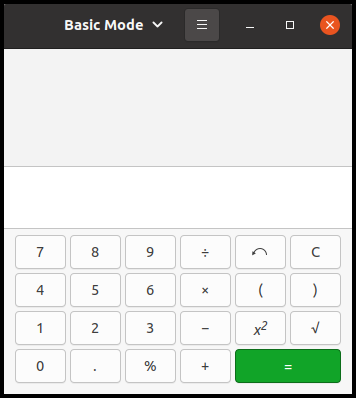
\includegraphics[width=5.34cm,height=5.97cm]{../image/gnome_calculator_basic.png}
\caption{gnome-calculator basic mode}
\end{figure}

Then, change the mode to advanced and quit.

\begin{figure}
\centering
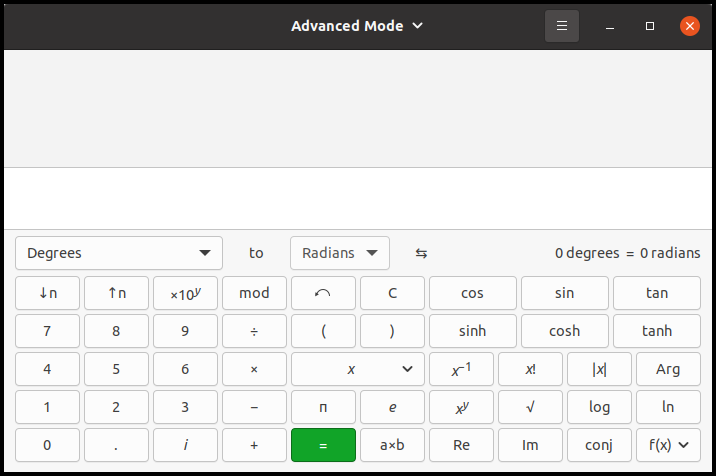
\includegraphics[width=10.74cm,height=7.14cm]{../image/gnome_calculator_advanced.png}
\caption{gnome-calculator advanced mode}
\end{figure}

Run gsettings and check whether the value of
\passthrough{\lstinline!button-mode!} changes.

\begin{lstlisting}
$ gsettings list-recursively org.gnome.calculator

... ...

org.gnome.calculator button-mode 'advanced'

... ...
\end{lstlisting}

Now we know that Gnome Calculator used gsettings and it has set
\passthrough{\lstinline!button-mode!} key to ``advanced''. The value
remains even the calculator quits. So when the calculator is run again,
it will appear as an advanced mode calculator.

\hypertarget{glib-compile-schemas}{%
\subsubsection{glib-compile-schemas}\label{glib-compile-schemas}}

GSettings schemas are specified with an XML format. The XML schema files
must have the filename extension \passthrough{\lstinline!.gschema.xml!}.
The following is the XML schema file for the application
\passthrough{\lstinline!tfe!}.

\begin{lstlisting}[language=XML, numbers=left]
<?xml version="1.0" encoding="UTF-8"?>
<schemalist>
  <schema path="/com/github/ToshioCP/tfe/" id="com.github.ToshioCP.tfe">
    <key name="font" type="s">
      <default>'Monospace 12'</default>
      <summary>Font</summary>
      <description>The font to be used for textview.</description>
    </key>
  </schema>
</schemalist>
\end{lstlisting}

The filename is ``com.github.ToshioCP.tfe.gschema.xml''. Schema XML
filenames are usually the schema id followed by ``.gschema.xml'' suffix.
You can use different name from schema id, but it is not recommended.

\begin{itemize}
\tightlist
\item
  2: The top level element is \passthrough{\lstinline!<schemalist>!}.
\item
  3: schema tag has \passthrough{\lstinline!path!} and
  \passthrough{\lstinline!id!} attributes. A path determines where the
  settings are stored in the conceptual global tree of settings. An id
  identifies the schema.
\item
  4: Key tag has two attributes. Name is the name of the key. Type is
  the type of the value of the key and specified with
  \href{https://docs.gtk.org/glib/struct.VariantType.html}{GLib API
  Reference, VariantType}.
\item
  5: default value of the key \passthrough{\lstinline!font!} is
  \passthrough{\lstinline!Monospace 12!}.
\item
  6: Summery and description elements describes the key. They are
  optional, but it is recommended to add them in the XML file.
\end{itemize}

The XML file is compiled by glib-compile-schemas. When compiling,
\passthrough{\lstinline!glib-compile-schemas!} compiles all the XML
files which have ``.gschema.xml'' file extension in the directory given
as an argument. It converts the XML file into a binary file
\passthrough{\lstinline!gschemas.compiled!}. Suppose the XML file above
is under \passthrough{\lstinline!tfe6!} directory.

\begin{lstlisting}
$ glib-compile-schemas tfe6
\end{lstlisting}

Then, \passthrough{\lstinline!gschemas.compiled!} is generated under
\passthrough{\lstinline!tfe6!}. When you test your application, set
\passthrough{\lstinline!GSETTINGS\_SCHEMA\_DIR!} so that GSettings objet
can find \passthrough{\lstinline!gschemas.compiled!}.

\begin{lstlisting}
$ GSETTINGS_SCHEMA_DIR=(the directory gschemas.compiled is located):$GSETTINGS_SCHEMA_DIR (your application name)
\end{lstlisting}

This is because GSettings object searches
\passthrough{\lstinline!GSETTINGS\_SCHEMA\_DIR!} for
\passthrough{\lstinline!gschemas.compiled!}.

GSettings object looks for this file by the following process.

\begin{itemize}
\tightlist
\item
  It searches \passthrough{\lstinline!glib-2.0/schemas!} subdirectories
  of all the directories specified in the environment variable
  \passthrough{\lstinline!XDG\_DATA\_DIRS!}. Most common directory is
  \passthrough{\lstinline!/usr/share/glib-2.0/schemas!}.
\item
  If \passthrough{\lstinline!GSETTINGS\_SCHEMA\_DIR!} environment
  variable is defined, it searches all the directories specified in the
  variable. \passthrough{\lstinline!GSETTINGS\_SCHEMA\_DIR!} can specify
  multiple directories delimited by colon (:).
\end{itemize}

In the directories above, all the \passthrough{\lstinline!.gschema.xml!}
files are stored. Therefore, when you install your application, follow
the instruction below to install your schemas.

\begin{enumerate}
\def\labelenumi{\arabic{enumi}.}
\tightlist
\item
  Make \passthrough{\lstinline!.gschema.xml!} file.
\item
  Copy it to one of the directories above. For example,
  \passthrough{\lstinline!/usr/local/share/glib-2.0/schemas!}.
\item
  Run \passthrough{\lstinline!glib-compile-schemas!} on the directory
  above.
\end{enumerate}

\hypertarget{meson.build}{%
\subsubsection{Meson.build}\label{meson.build}}

Meson provides \passthrough{\lstinline!gnome.compile\_schemas!} method
to compile XML file in the build directory. This is used to test the
application. Write the following to the
\passthrough{\lstinline!meson.build!} file.

\begin{lstlisting}
gnome.compile_schemas(build_by_default: true, depend_files: 'com.github.ToshioCP.tfe.gschema.xml')
\end{lstlisting}

\begin{itemize}
\tightlist
\item
  \passthrough{\lstinline!build\_by\_default!}: If it is true, the
  target will be build by default.
\item
  \passthrough{\lstinline!depend\_files!}: XML files to be compiled.
\end{itemize}

In the example above, this method runs
\passthrough{\lstinline!glib-compile-schemas!} to generate
\passthrough{\lstinline!gschemas.compiled!} from the XML file
\passthrough{\lstinline!com.github.ToshioCP.tfe.gschema.xml!}. The file
\passthrough{\lstinline!gschemas.compiled!} is located under the build
directory. If you run meson as \passthrough{\lstinline!meson \_build!}
and ninja as \passthrough{\lstinline!ninja -C \_build!}, then it is
under \passthrough{\lstinline!\_build!} directory.

After compilation, you can test your application like this:

\begin{lstlisting}
$ GSETTINGS_SCHEMA_DIR=_build:$GSETTINGS_SCHEMA_DIR _build/tfe
\end{lstlisting}

\hypertarget{gsettings-object-and-g_settings_bind}{%
\subsubsection{GSettings object and
g\_settings\_bind}\label{gsettings-object-and-g_settings_bind}}

Write gsettings related codes to `tfeapplication.c'.

\begin{lstlisting}[language=C]
... ...
static GSettings *settings;
... ...

void
tfe_application_quit (GtkWindow *win) {
  ... ...
  g_clear_object (&settings);
  ... ...
}

static void
tfe_startup (GApplication *application) {
  ... ...
  settings = g_settings_new ("com.github.ToshioCP.tfe");
  g_settings_bind (settings, "font", fontbtn, "font", G_SETTINGS_BIND_DEFAULT);
  ... ...
}
\end{lstlisting}

Static variable \passthrough{\lstinline!settings!} keeps a pointer to
GSettings instance. Before application quits, the application releases
the GSettings instance. The function
\passthrough{\lstinline!g\_clear\_object!} is used.

Startup handler creates GSettings instance with the schema id
``com.github.ToshioCP.tfe'' and assigns the pointer to
\passthrough{\lstinline!settings!}. The function
\passthrough{\lstinline!g\_settings\_bind!} connects the settings keys
(key and value) and the ``font'' property of
\passthrough{\lstinline!fontbtn!}. Then the two values will be always
the same. If one value changes then the other will automatically change.

You need to make an effort to understand GSettings concept, but coding
is very simple. Just create a GSettings object and bind it to a property
of an object.

\hypertarget{installation}{%
\subsection{Installation}\label{installation}}

It is a good idea to install your application in
\passthrough{\lstinline!$HOME/local/bin!} directory if you have
installed Gtk4 from the source (See Section 2). Then you need to put
\passthrough{\lstinline!--prefix=$HOME/local!} option to meson like
this.

\begin{lstlisting}
$ meson --prefix=$HOME/local _build
\end{lstlisting}

If you've installed Gtk4 from the distribution package,
\passthrough{\lstinline!--prefix!} option isn't necessary. You just
install \passthrough{\lstinline!tfe!} to the default bin directory like
\passthrough{\lstinline!/usr/local/bin!}.

Modify \passthrough{\lstinline!meson.build!} and add install option and
set it true in executable function.

\begin{lstlisting}
executable('tfe', sourcefiles, resources, dependencies: gtkdep, export_dynamic: true, install: true)
\end{lstlisting}

You can install your application by:

\begin{lstlisting}
$ ninja -C _build install
\end{lstlisting}

However, you need to do one more thing. Copy your XML file to
\passthrough{\lstinline!$HOME/local/share/glib-2.0/schemas/!}, which is
specified in \passthrough{\lstinline!GSETTINGS\_SCHEMA\_DIR!}
environment variable, and run
\passthrough{\lstinline!glib-compile-schemas!} on that directory.

\begin{lstlisting}
schema_dir = get_option('prefix') / get_option('datadir') / 'glib-2.0/schemas/'
install_data('com.github.ToshioCP.tfe.gschema.xml', install_dir: schema_dir)
\end{lstlisting}

\begin{itemize}
\tightlist
\item
  get\_option: This function returns the value of build options. The
  default value of the option `prefix' is ``/usr/local'', but it is
  ``\$HOME/local'' because we have run meson with prefix option. The
  default value of the option `datadir' is ``share''. The operator `/'
  connects the strings with `/' separator. So,
  \passthrough{\lstinline!$HOME/local/share/glib-2.0/schemas!} is
  assigned to the variable \passthrough{\lstinline!schema\_dir!}.
\item
  install\_data: This function installs the data to the install
  directory.
\end{itemize}

Meson can run a post compile script.

\begin{lstlisting}
meson.add_install_script('glib-compile-schemas', schema_dir)
\end{lstlisting}

This method runs `glib-compile-schemas' with an argument
\passthrough{\lstinline!schema\_dir!}. The following is
\passthrough{\lstinline!meson.build!}.

\begin{lstlisting}[numbers=left]
project('tfe', 'c')

gtkdep = dependency('gtk4')

gnome=import('gnome')
resources = gnome.compile_resources('resources','tfe.gresource.xml')
gnome.compile_schemas(build_by_default: true, depend_files: 'com.github.ToshioCP.tfe.gschema.xml')

sourcefiles=files('tfeapplication.c', 'tfenotebook.c', 'css.c', '../tfetextview/tfetextview.c')

executable('tfe', sourcefiles, resources, dependencies: gtkdep, export_dynamic: true, install: true)

schema_dir = get_option('prefix') / get_option('datadir') / 'glib-2.0/schemas/'
install_data('com.github.ToshioCP.tfe.gschema.xml', install_dir: schema_dir)
meson.add_install_script('glib-compile-schemas', schema_dir)
\end{lstlisting}

Source files of \passthrough{\lstinline!tfe!} is under src/tfe6
directory. Copy them to your temporary directory and try to compile and
install.

\begin{lstlisting}
$ meson --prefix=$HOME/local _build
$ ninja -C _build
$ GSETTINGS_SCHEMA_DIR=_build:$GSETTINGS_SCHEMA_DIR _build/tfe
$ ninja -C _build install
$ tfe
$ ls $HOME/local/bin
... ...
... tfe
... ...
$ ls $HOME/local/share/glib-2.0/schemas
com.github.ToshioCP.tfe.gschema.xml
gschema.dtd
gschemas.compiled
... ...
\end{lstlisting}

The screenshot is as follows.

\begin{figure}
\centering
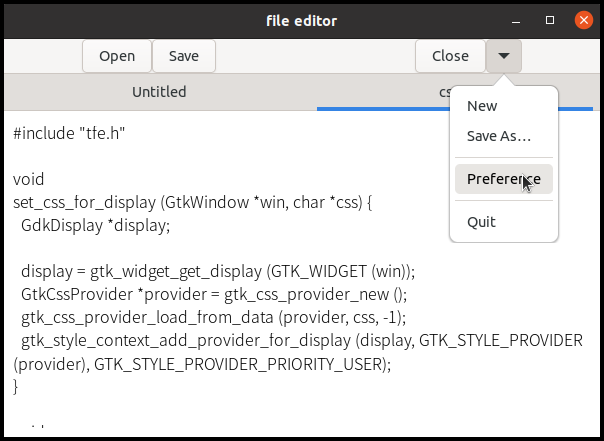
\includegraphics[width=9.06cm,height=6.615cm]{../image/tfe6.png}
\caption{tfe6}
\end{figure}

  \hypertarget{template-xml-and-composite-widget}{%
\section{Template XML and composite
widget}\label{template-xml-and-composite-widget}}

The tfe program in the previous section is not so good because many
things are crammed into \passthrough{\lstinline!tfepplication.c!}. Many
static variables in \passthrough{\lstinline!tfepplication.c!} shows
that.

\begin{lstlisting}[language=C]
static GtkDialog *pref;
static GtkFontButton *fontbtn;
static GSettings *settings;
static GtkDialog *alert;
static GtkLabel *lb_alert;
static GtkButton *btn_accept;

static gulong pref_close_request_handler_id = 0;
static gulong alert_close_request_handler_id = 0;
static gboolean is_quit;
\end{lstlisting}

Generally, if there are many global or static variables in the program,
it is not a good program. Such programs are difficult to maintain.

The file \passthrough{\lstinline!tfeapplication.c!} should be divided
into several files.

\begin{itemize}
\tightlist
\item
  \passthrough{\lstinline!tfeapplication.c!} only has codes related to
  GtkApplication.
\item
  A file for GtkApplicationWindow
\item
  A file for a preference dialog
\item
  A file for an alert dialog
\end{itemize}

The preference dialog is defined by a ui file. And it has GtkBox,
GtkLabel and GtkFontButton in it. Such widget is called composite
widget. Composite widget is a child object (not child widget) of a
widget. For example, the preference composite widget is a child object
of GtkDialog. Composite widget can be built from template XML. Next
subsection shows how to build a preference dialog.

\hypertarget{preference-dialog}{%
\subsection{Preference dialog}\label{preference-dialog}}

First, write a template XML file.

\begin{lstlisting}[language=XML, numbers=left]
<?xml version="1.0" encoding="UTF-8"?>
<interface>
  <template class="TfePref" parent="GtkDialog">
    <property name="title">Preferences</property>
    <property name="resizable">FALSE</property>
    <property name="modal">TRUE</property>
    <child internal-child="content_area">
      <object class="GtkBox" id="content_area">
        <child>
          <object class="GtkBox" id="pref_boxh">
            <property name="orientation">GTK_ORIENTATION_HORIZONTAL</property>
            <property name="spacing">12</property>
            <property name="margin-start">12</property>
            <property name="margin-end">12</property>
            <property name="margin-top">12</property>
            <property name="margin-bottom">12</property>
            <child>
              <object class="GtkLabel" id="fontlabel">
                <property name="label">Font:</property>
                <property name="xalign">1</property>
              </object>
            </child>
            <child>
              <object class="GtkFontButton" id="fontbtn">
              </object>
            </child>
          </object>
        </child>
      </object>
    </child>
  </template>
</interface>
\end{lstlisting}

\begin{itemize}
\tightlist
\item
  3: Template tag specifies a composite widget. The value of a class
  attribute is the object name of the composite widget. This XML file
  names the object ``TfePref''. It is defined in a C source file and it
  will be shown later. A parent attribute specifies the direct parent
  object of the composite widget. \passthrough{\lstinline!TfePref!} is a
  child object of \passthrough{\lstinline!GtkDialog!}. Therefore the
  value of the attribute is ``GtkDialog''. A parent attribute is
  optional but it is recommended to specify.
\end{itemize}

Other lines are the same as before. The object
\passthrough{\lstinline!TfePref!} is defined in
\passthrough{\lstinline!tfepref.h!} and
\passthrough{\lstinline!tfepref.c!}.

\begin{lstlisting}[language=C, numbers=left]
#ifndef __TFE_PREF_H__
#define __TFE_PREF_H__

#include <gtk/gtk.h>

#define TFE_TYPE_PREF tfe_pref_get_type ()
G_DECLARE_FINAL_TYPE (TfePref, tfe_pref, TFE, PREF, GtkDialog)

GtkWidget *
tfe_pref_new (GtkWindow *win);

#endif /* __TFE_PREF_H__ */
\end{lstlisting}

\begin{itemize}
\tightlist
\item
  6-7: When you define a new object, you need to write these two lines.
  Refer to Section 8.
\item
  9-10: \passthrough{\lstinline!tfe\_pref\_new!} creates a new TfePref
  object. It has a parameter \passthrough{\lstinline!win!} which is used
  as a transient parent window to show the dialog.
\end{itemize}

\begin{lstlisting}[language=C, numbers=left]
#include "tfepref.h"

struct _TfePref
{
  GtkDialog parent;
  GSettings *settings;
  GtkFontButton *fontbtn;
};

G_DEFINE_TYPE (TfePref, tfe_pref, GTK_TYPE_DIALOG);

static void
tfe_pref_dispose (GObject *gobject) {
  TfePref *pref = TFE_PREF (gobject);

  g_clear_object (&pref->settings);
  G_OBJECT_CLASS (tfe_pref_parent_class)->dispose (gobject);
}

static void
tfe_pref_init (TfePref *pref) {
  gtk_widget_init_template (GTK_WIDGET (pref));
  pref->settings = g_settings_new ("com.github.ToshioCP.tfe");
  g_settings_bind (pref->settings, "font", pref->fontbtn, "font", G_SETTINGS_BIND_DEFAULT);
}

static void
tfe_pref_class_init (TfePrefClass *class) {
  GObjectClass *object_class = G_OBJECT_CLASS (class);

  object_class->dispose = tfe_pref_dispose;
  gtk_widget_class_set_template_from_resource (GTK_WIDGET_CLASS (class), "/com/github/ToshioCP/tfe/tfepref.ui");
  gtk_widget_class_bind_template_child (GTK_WIDGET_CLASS (class), TfePref, fontbtn);
}

GtkWidget *
tfe_pref_new (GtkWindow *win) {
  return GTK_WIDGET (g_object_new (TFE_TYPE_PREF, "transient-for", win, NULL));
}
\end{lstlisting}

\begin{itemize}
\tightlist
\item
  3-8: The structure of an instance of this object. It has two
  variables, settings and fontbtn.
\item
  10: \passthrough{\lstinline!G\_DEFINE\_TYPE!} macro. This macro
  registers the TfePref type.
\item
  12-18: Dispose handler. This handler is called when the instance is
  destroyed. The destruction process has two stages, disposing and
  finalizing. When disposing, the instance releases all the references
  (to the other instances). TfePref object holds a reference to the
  GSettings instance. It is released in line 16. After that parents
  dispose handler is called in line 17. For further information about
  destruction process, refer to Section 11.
\item
  27-34: Class initialization function.
\item
  31: Set the dispose handler.
\item
  32:
  \passthrough{\lstinline!gtk\_widget\_class\_set\_template\_from\_resource!}
  function associates the description in the XML file
  (\passthrough{\lstinline!tfepref.ui!}) with the widget. At this moment
  no instance is created. It just make the class to know the structure
  of the object. That's why the top level tag is not
  \passthrough{\lstinline!<object>!} but
  \passthrough{\lstinline!<template>!} in the XML file.
\item
  33:
  \passthrough{\lstinline!gtk\_widget\_class\_bind\_template\_child!}
  function binds a private variable of the object with a child object in
  the template. This function is a macro. The name of the private
  variable (\passthrough{\lstinline!fontbtn!} in line 7) and the id
  \passthrough{\lstinline!fontbtn!} in the XML file (line 24) must be
  the same. The pointer to the instance will be assigned to the variable
  \passthrough{\lstinline!fontbtn!} when the instance is created.
\item
  20-25: Instance initialization function.
\item
  22: Creates the instance based on the template in the class. The
  template has been made during the class initialization process.
\item
  23: Create GSettings instance with the id ``com.github.ToshioCP.tfe''.
\item
  24: Bind the font key in the GSettings object to the font property in
  the GtkFontButton.
\item
  36-39: The function \passthrough{\lstinline!tfe\_pref\_new!} creates
  an instance of TfePref. The parameter \passthrough{\lstinline!win!} is
  a transient parent.
\end{itemize}

Now, It is very simple to use this dialog. A caller just creates this
object and shows it.

\begin{lstlisting}[language=C]
TfePref *pref;
pref = tfe_pref_new (win) /* win is the top-level window */
gtk_widget_show (GTK_WINDOW (win));
\end{lstlisting}

This instance is automatically destroyed when a user clicks on the close
button. That's all. If you want to show the dialog again, just create
and show it.

\hypertarget{alert-dialog}{%
\subsection{Alert dialog}\label{alert-dialog}}

It is almost same as preference dialog.

Its XML file is:

\begin{lstlisting}[language=XML, numbers=left]
<?xml version="1.0" encoding="UTF-8"?>
<interface>
  <template class="TfeAlert" parent="GtkDialog">
    <property name="title">Are you sure?</property>
    <property name="resizable">FALSE</property>
    <property name="modal">TRUE</property>
    <child internal-child="content_area">
      <object class="GtkBox">
        <child>
          <object class="GtkBox">
            <property name="orientation">GTK_ORIENTATION_HORIZONTAL</property>
            <property name="spacing">12</property>
            <property name="margin-start">12</property>
            <property name="margin-end">12</property>
            <property name="margin-top">12</property>
            <property name="margin-bottom">12</property>
            <child>
              <object class="GtkImage">
                <property name="icon-name">dialog-warning</property>
                <property name="icon-size">GTK_ICON_SIZE_LARGE</property>
              </object>
            </child>
            <child>
              <object class="GtkLabel" id="lb_alert">
              </object>
            </child>
          </object>
        </child>
      </object>
    </child>
    <child type="action">
      <object class="GtkButton" id="btn_cancel">
        <property name="label">Cancel</property>
      </object>
    </child>
    <child type="action">
      <object class="GtkButton" id="btn_accept">
        <property name="label">Close</property>
      </object>
    </child>
    <action-widgets>
      <action-widget response="cancel" default="true">btn_cancel</action-widget>
      <action-widget response="accept">btn_accept</action-widget>
    </action-widgets>
  </template>
</interface>
\end{lstlisting}

The header file is:

\begin{lstlisting}[language=C, numbers=left]
#ifndef __TFE_ALERT_H__
#define __TFE_ALERT_H__

#include <gtk/gtk.h>

#define TFE_TYPE_ALERT tfe_alert_get_type ()
G_DECLARE_FINAL_TYPE (TfeAlert, tfe_alert, TFE, ALERT, GtkDialog)

void
tfe_alert_set_message (TfeAlert *alert, const char *message);

void
tfe_alert_set_button_label (TfeAlert *alert, const char *label);

GtkWidget *
tfe_alert_new (GtkWindow *win);

#endif /* __TFE_ALERT_H__ */
\end{lstlisting}

There are three public functions. The functions
\passthrough{\lstinline!tfe\_alert\_set\_message!} and
\passthrough{\lstinline!tfe\_alert\_set\_button\_label!} sets the label
and button name of the alert dialog. For example, if you want to show an
alert that the user tries to close without saving the content, set them
like:

\begin{lstlisting}[language=C]
tfe_alert_set_message (alert, "Are you really close without saving?"); /* alert points to a TfeAlert instance */
tfe_alert_set_button_label (alert, "Close");
\end{lstlisting}

The function \passthrough{\lstinline!tfe\_alert\_new!} creates a
TfeAlert dialog.

The C source file is:

\begin{lstlisting}[language=C, numbers=left]
#include "tfealert.h"

struct _TfeAlert
{
  GtkDialog parent;
  GtkLabel *lb_alert;
  GtkButton *btn_accept;
};

G_DEFINE_TYPE (TfeAlert, tfe_alert, GTK_TYPE_DIALOG);

void
tfe_alert_set_message (TfeAlert *alert, const char *message) {
  gtk_label_set_text (alert->lb_alert, message);
}

void
tfe_alert_set_button_label (TfeAlert *alert, const char *label) {
  gtk_button_set_label (alert->btn_accept, label);
}

static void
tfe_alert_init (TfeAlert *alert) {
  gtk_widget_init_template (GTK_WIDGET (alert));
}

static void
tfe_alert_class_init (TfeAlertClass *class) {
  gtk_widget_class_set_template_from_resource (GTK_WIDGET_CLASS (class), "/com/github/ToshioCP/tfe/tfealert.ui");
  gtk_widget_class_bind_template_child (GTK_WIDGET_CLASS (class), TfeAlert, lb_alert);
  gtk_widget_class_bind_template_child (GTK_WIDGET_CLASS (class), TfeAlert, btn_accept);
}

GtkWidget *
tfe_alert_new (GtkWindow *win) {
  return GTK_WIDGET (g_object_new (TFE_TYPE_ALERT, "transient-for", win, NULL));
}
\end{lstlisting}

The program is almost same as \passthrough{\lstinline!tfepref.c!}.

The instruction how to use this object is as follows.

\begin{enumerate}
\def\labelenumi{\arabic{enumi}.}
\tightlist
\item
  Write a ``response'' signal handler.
\item
  Create a TfeAlert object.
\item
  Connect ``response'' signal to a handler
\item
  Show the dialog
\item
  In the signal handler, do something with regard to the response-id.
  Then destroy the dialog.
\end{enumerate}

\hypertarget{top-level-window}{%
\subsection{Top-level window}\label{top-level-window}}

In the same way, create a child object of GtkApplicationWindow. The
object name is ``TfeWindow''.

\begin{lstlisting}[language=XML, numbers=left]
<?xml version="1.0" encoding="UTF-8"?>
<interface>
  <template class="TfeWindow" parent="GtkApplicationWindow">
    <property name="title">file editor</property>
    <property name="default-width">600</property>
    <property name="default-height">400</property>
    <child>
      <object class="GtkBox" id="boxv">
        <property name="orientation">GTK_ORIENTATION_VERTICAL</property>
        <child>
          <object class="GtkBox" id="boxh">
            <property name="orientation">GTK_ORIENTATION_HORIZONTAL</property>
            <child>
              <object class="GtkLabel" id="dmy1">
                <property name="width-chars">10</property>
              </object>
            </child>
            <child>
              <object class="GtkButton" id="btno">
                <property name="label">Open</property>
                <property name="action-name">win.open</property>
              </object>
            </child>
            <child>
              <object class="GtkButton" id="btns">
                <property name="label">Save</property>
                <property name="action-name">win.save</property>
              </object>
            </child>
            <child>
              <object class="GtkLabel" id="dmy2">
                <property name="hexpand">TRUE</property>
              </object>
            </child>
            <child>
              <object class="GtkButton" id="btnc">
                <property name="label">Close</property>
                <property name="action-name">win.close</property>
              </object>
            </child>
            <child>
              <object class="GtkMenuButton" id="btnm">
                <property name="direction">down</property>
                <property name="halign">start</property>
                <property name="icon-name">open-menu-symbolic</property>
              </object>
            </child>
            <child>
              <object class="GtkLabel" id="dmy3">
                <property name="width-chars">10</property>
              </object>
            </child>
          </object>
        </child>
        <child>
          <object class="GtkNotebook" id="nb">
            <property name="scrollable">TRUE</property>
            <property name="hexpand">TRUE</property>
            <property name="vexpand">TRUE</property>
          </object>
        </child>
      </object>
    </child>
  </template>
</interface>
\end{lstlisting}

This XML file is almost same as before except template tag and
``action-name'' property in buttons.

GtkButton implements GtkActionable interface, which has ``action-name''
property. If this property is set, GtkButton activates the action when
it is clicked. For example, if an open button is clicked, ``win.open''
action will be activated and \passthrough{\lstinline!open\_activated!}
handler will be invoked.

This action is also used by ``\textless Control\textgreater o''
accelerator (See the source code of
\passthrough{\lstinline!tfewindow.c!} below). If you use ``clicked''
signal for the button, you need its signal handler. Then, there are two
handlers:

\begin{itemize}
\tightlist
\item
  a handler for the ``clicked'' signal on the button
\item
  a handler for the ``activate'' signal on the ``win.open'' action, to
  which ``\textless Control\textgreater o'' accelerator is connected
\end{itemize}

These two handlers do almost same thing. It is inefficient. Connecting
buttons to actions is a good way to reduce unnecessary codes.

\begin{lstlisting}[language=C, numbers=left]
#ifndef __TFE_WINDOW_H__
#define __TFE_WINDOW_H__

#include <gtk/gtk.h>

#define TFE_TYPE_WINDOW tfe_window_get_type ()
G_DECLARE_FINAL_TYPE (TfeWindow, tfe_window, TFE, WINDOW, GtkApplicationWindow)

void
tfe_window_notebook_page_new (TfeWindow *win);

void
tfe_window_notebook_page_new_with_files (TfeWindow *win, GFile **files, int n_files);

GtkWidget *
tfe_window_new (GtkApplication *app);

#endif /* __TFE_WINDOW_H__ */
\end{lstlisting}

There are three public functions. The function
\passthrough{\lstinline!tfe\_window\_notebook\_page\_new!} creates a new
notebook page. This is a wrapper function for
\passthrough{\lstinline!notebook\_page\_new!}. It is called by
GtkApplication object. The function
\passthrough{\lstinline!tfe\_window\_notebook\_page\_new\_with\_files!}
creates notebook pages with a contents read from the given files. The
function \passthrough{\lstinline!tfe\_window\_new!} creates a TfeWindow
instance.

\begin{lstlisting}[language=C, numbers=left]
#include "tfewindow.h"
#include "tfenotebook.h"
#include "tfepref.h"
#include "tfealert.h"
#include "css.h"

struct _TfeWindow {
  GtkApplicationWindow parent;
  GtkMenuButton *btnm;
  GtkNotebook *nb;
  GSettings *settings;
  gboolean is_quit;
};

G_DEFINE_TYPE (TfeWindow, tfe_window, GTK_TYPE_APPLICATION_WINDOW);

/* alert response signal handler */
static void
alert_response_cb (GtkDialog *alert, int response_id, gpointer user_data) {
  TfeWindow *win = TFE_WINDOW (user_data);

  if (response_id == GTK_RESPONSE_ACCEPT) {
    if (win->is_quit)
      gtk_window_destroy(GTK_WINDOW (win));
    else
      notebook_page_close (win->nb);
  }
  gtk_window_destroy (GTK_WINDOW (alert));
}

/* ----- action activated handlers ----- */
static void
open_activated (GSimpleAction *action, GVariant *parameter, gpointer user_data) {
  TfeWindow *win = TFE_WINDOW (user_data);

  notebook_page_open (GTK_NOTEBOOK (win->nb));
}

static void
save_activated (GSimpleAction *action, GVariant *parameter, gpointer user_data) {
  TfeWindow *win = TFE_WINDOW (user_data);

  notebook_page_save (GTK_NOTEBOOK (win->nb));
}

static void
close_activated (GSimpleAction *action, GVariant *parameter, gpointer user_data) {
  TfeWindow *win = TFE_WINDOW (user_data);
  TfeAlert *alert;

  if (has_saved (win->nb))
    notebook_page_close (win->nb);
  else {
    win->is_quit = false;
    alert = TFE_ALERT (tfe_alert_new (GTK_WINDOW (win)));
    tfe_alert_set_message (alert, "Contents aren't saved yet.\nAre you sure to close?");
    tfe_alert_set_button_label (alert, "Close");
    g_signal_connect (GTK_DIALOG (alert), "response", G_CALLBACK (alert_response_cb), win);
    gtk_widget_show (GTK_WIDGET (alert));
  }
}

static void
new_activated (GSimpleAction *action, GVariant *parameter, gpointer user_data) {
  TfeWindow *win = TFE_WINDOW (user_data);

  notebook_page_new (GTK_NOTEBOOK (win->nb));
}

static void
saveas_activated (GSimpleAction *action, GVariant *parameter, gpointer user_data) {
  TfeWindow *win = TFE_WINDOW (user_data);

  notebook_page_saveas (GTK_NOTEBOOK (win->nb));
}

static void
pref_activated (GSimpleAction *action, GVariant *parameter, gpointer user_data) {
  TfeWindow *win = TFE_WINDOW (user_data);
  GtkWidget *pref;

  pref = tfe_pref_new (GTK_WINDOW (win));
  gtk_widget_show (pref);
}

static void
quit_activated (GSimpleAction *action, GVariant *parameter, gpointer user_data) {
  TfeWindow *win = TFE_WINDOW (user_data);

  TfeAlert *alert;

  if (has_saved_all (GTK_NOTEBOOK (win->nb)))
    gtk_window_destroy (GTK_WINDOW (win));
  else {
    win->is_quit = true;
    alert = TFE_ALERT (tfe_alert_new (GTK_WINDOW (win)));
    tfe_alert_set_message (alert, "Contents aren't saved yet.\nAre you sure to quit?");
    tfe_alert_set_button_label (alert, "Quit");
    g_signal_connect (GTK_DIALOG (alert), "response", G_CALLBACK (alert_response_cb), win);
    gtk_widget_show (GTK_WIDGET (alert));
  }
}

/* gsettings changed::font signal handler */
static void
changed_font_cb (GSettings *settings, char *key, gpointer user_data) {
  GtkWindow *win = GTK_WINDOW (user_data); 
  char *font;
  PangoFontDescription *pango_font_desc;

  font = g_settings_get_string (settings, "font");
  pango_font_desc = pango_font_description_from_string (font);
  g_free (font);
  set_font_for_display_with_pango_font_desc (win, pango_font_desc);
}

/* --- public functions --- */

void
tfe_window_notebook_page_new (TfeWindow *win) {
  notebook_page_new (win->nb);
}

void
tfe_window_notebook_page_new_with_files (TfeWindow *win, GFile **files, int n_files) {
  int i;

  for (i = 0; i < n_files; i++)
    notebook_page_new_with_file (win->nb, files[i]);
  if (gtk_notebook_get_n_pages (win->nb) == 0)
    notebook_page_new (win->nb);
}

/* --- TfeWindow object construction/destruction --- */ 
static void
tfe_window_dispose (GObject *gobject) {
  TfeWindow *window = TFE_WINDOW (gobject);

  g_clear_object (&window->settings);
  G_OBJECT_CLASS (tfe_window_parent_class)->dispose (gobject);
}

static void
tfe_window_init (TfeWindow *win) {
  GtkBuilder *build;
  GMenuModel *menu;

  gtk_widget_init_template (GTK_WIDGET (win));

  build = gtk_builder_new_from_resource ("/com/github/ToshioCP/tfe/menu.ui");
  menu = G_MENU_MODEL (gtk_builder_get_object (build, "menu"));
  gtk_menu_button_set_menu_model (win->btnm, menu);
  g_object_unref(build);

  win->settings = g_settings_new ("com.github.ToshioCP.tfe");
  g_signal_connect (win->settings, "changed::font", G_CALLBACK (changed_font_cb), win);

/* ----- action ----- */
  const GActionEntry win_entries[] = {
    { "open", open_activated, NULL, NULL, NULL },
    { "save", save_activated, NULL, NULL, NULL },
    { "close", close_activated, NULL, NULL, NULL },
    { "new", new_activated, NULL, NULL, NULL },
    { "saveas", saveas_activated, NULL, NULL, NULL },
    { "pref", pref_activated, NULL, NULL, NULL },
    { "close-all", quit_activated, NULL, NULL, NULL }
  };
  g_action_map_add_action_entries (G_ACTION_MAP (win), win_entries, G_N_ELEMENTS (win_entries), win);

  changed_font_cb(win->settings, "font", win);
}

static void
tfe_window_class_init (TfeWindowClass *class) {
  GObjectClass *object_class = G_OBJECT_CLASS (class);

  object_class->dispose = tfe_window_dispose;
  gtk_widget_class_set_template_from_resource (GTK_WIDGET_CLASS (class), "/com/github/ToshioCP/tfe/tfewindow.ui");
  gtk_widget_class_bind_template_child (GTK_WIDGET_CLASS (class), TfeWindow, btnm);
  gtk_widget_class_bind_template_child (GTK_WIDGET_CLASS (class), TfeWindow, nb);
}

GtkWidget *
tfe_window_new (GtkApplication *app) {
  return GTK_WIDGET (g_object_new (TFE_TYPE_WINDOW, "application", app, NULL));
}
\end{lstlisting}

\begin{itemize}
\tightlist
\item
  17-29: \passthrough{\lstinline!alert\_response\_cb!} is a call back
  function of the ``response'' signal of TfeAlert dialog. This is the
  same as before except
  \passthrough{\lstinline!gtk\_window\_destroy(GTK\_WINDOW (win))!} is
  used instead of \passthrough{\lstinline!tfe\_application\_quit!}.
\item
  31-102: Handlers of action activated signal. The
  \passthrough{\lstinline!user\_data!} is a pointer to TfeWindow
  instance.
\item
  104-115: A handler of ``changed::font'' signal of GSettings object.
\item
  111: Gets the font from GSettings data.
\item
  112: Gets a PangoFontDescription from the font. In the previous
  version, the program gets the font description from the GtkFontButton.
  The button data and GSettings data are the same. Therefore, the data
  got here is the same as the data in the GtkFontButton. In addition, we
  don't need to worry about the preference dialog is alive or not thanks
  to the GSettings.
\item
  114: Sets CSS on the display with the font description.
\item
  117-132: Public functions.
\item
  134-141: Dispose handler. The GSettings object needs to be released.
\item
  143-171: Instance initialization function.
\item
  148: Creates a composite widget instance with the template.
\item
  151-153: Insert \passthrough{\lstinline!menu!} to the menu button.
\item
  155-156: Creates a GSettings instance with the id
  ``com.github.ToshioCP.tfe''. Connects ``changed::font'' signal to the
  handler \passthrough{\lstinline!changed\_font\_cb!}. This signal emits
  when the GSettings data is changed. The second part ``font'' of the
  signal name ``changed::font'' is called details. Signals can have
  details. If a GSettings instance has more than one key, ``changed''
  signal emits only if the key, which has the same name as the detail,
  changes its value. For example, Suppose a GSettings object has three
  keys ``a'', ``b'' and ``c''.

  \begin{itemize}
  \tightlist
  \item
    ``changed::a'' is emitted when the value of the key ``a'' is
    changed. It isn't emitted when the value of ``b'' or ``c'' is
    changed.
  \item
    ``changed::b'' is emitted when the value of the key ``b'' is
    changed. It isn't emitted when the value of ``a'' or ``c'' is
    changed.
  \item
    ``changed::c'' is emitted when the value of the key ``c'' is
    changed. It isn't emitted when the value of ``a'' or ``b'' is
    changed. In this version of tfe, there is only one key (``font'').
    So, even if the signal doesn't have a detail, the result is the
    same. But in the future version, it will probably need details.
  \end{itemize}
\item
  158-168: Creates actions.
\item
  170: Sets CSS font.
\item
  173-181: Class initialization function.
\item
  177: Sets the dispose handler.
\item
  178: Sets the composite widget template
\item
  179-180: Binds private variable with child objects in the template.
\item
  183-186: \passthrough{\lstinline!tfe\_window\_new!}. This function
  creates TfeWindow instance.
\end{itemize}

\hypertarget{tfeapplication}{%
\subsection{TfeApplication}\label{tfeapplication}}

The file \passthrough{\lstinline!tfeapplication.c!} is now very simple.

\begin{lstlisting}[language=C, numbers=left]
#include "tfewindow.h"

/* ----- activate, open, startup handlers ----- */
static void
app_activate (GApplication *application) {
  GtkApplication *app = GTK_APPLICATION (application);
  GtkWidget *win = GTK_WIDGET (gtk_application_get_active_window (app));

  tfe_window_notebook_page_new (TFE_WINDOW (win));
  gtk_widget_show (GTK_WIDGET (win));
}

static void
app_open (GApplication *application, GFile ** files, gint n_files, const gchar *hint) {
  GtkApplication *app = GTK_APPLICATION (application);
  GtkWidget *win = GTK_WIDGET (gtk_application_get_active_window (app));

  tfe_window_notebook_page_new_with_files (TFE_WINDOW (win), files, n_files);
  gtk_widget_show (win);
}

static void
app_startup (GApplication *application) {
  GtkApplication *app = GTK_APPLICATION (application);
  int i;

  tfe_window_new (app);

/* ----- accelerator ----- */ 
  struct {
    const char *action;
    const char *accels[2];
  } action_accels[] = {
    { "win.open", { "<Control>o", NULL } },
    { "win.save", { "<Control>s", NULL } },
    { "win.close", { "<Control>w", NULL } },
    { "win.new", { "<Control>n", NULL } },
    { "win.saveas", { "<Shift><Control>s", NULL } },
    { "win.close-all", { "<Control>q", NULL } },
  };

  for (i = 0; i < G_N_ELEMENTS(action_accels); i++)
    gtk_application_set_accels_for_action(GTK_APPLICATION(app), action_accels[i].action, action_accels[i].accels);
}

/* ----- main ----- */

#define APPLICATION_ID "com.github.ToshioCP.tfe"

int
main (int argc, char **argv) {
  GtkApplication *app;
  int stat;

  app = gtk_application_new (APPLICATION_ID, G_APPLICATION_HANDLES_OPEN);

  g_signal_connect (app, "startup", G_CALLBACK (app_startup), NULL);
  g_signal_connect (app, "activate", G_CALLBACK (app_activate), NULL);
  g_signal_connect (app, "open", G_CALLBACK (app_open), NULL);

  stat =g_application_run (G_APPLICATION (app), argc, argv);
  g_object_unref (app);
  return stat;
}
\end{lstlisting}

\begin{itemize}
\tightlist
\item
  4-11: Activate signal handler. It uses
  \passthrough{\lstinline!tfe\_window\_notebook\_page\_new!} instead of
  \passthrough{\lstinline!notebook\_page\_new!}.
\item
  13-20: Open signal handler. Thanks to
  \passthrough{\lstinline!tfe\_window\_notebook\_page\_new\_with\_files!},
  this handler becomes very simple.
\item
  22-44: Startup signal handler. Most of the tasks are moved to
  TfeWindow, the remaining tasks are creating a window and setting
  accelerations.
\item
  48-64: A function \passthrough{\lstinline!main!}.
\end{itemize}

\hypertarget{other-files}{%
\subsection{Other files}\label{other-files}}

Resource XML file.

\begin{lstlisting}[language=XML, numbers=left]
<?xml version="1.0" encoding="UTF-8"?>
<gresources>
  <gresource prefix="/com/github/ToshioCP/tfe">
    <file>tfewindow.ui</file>
    <file>tfepref.ui</file>
    <file>tfealert.ui</file>
    <file>menu.ui</file>
  </gresource>
</gresources>
\end{lstlisting}

GSchema XML file

\begin{lstlisting}[language=XML, numbers=left]
<?xml version="1.0" encoding="UTF-8"?>
<schemalist>
  <schema path="/com/github/ToshioCP/tfe/" id="com.github.ToshioCP.tfe">
    <key name="font" type="s">
      <default>'Monospace 12'</default>
      <summary>Font</summary>
      <description>The font to be used for textview.</description>
    </key>
  </schema>
</schemalist>
\end{lstlisting}

Meson.build

\begin{lstlisting}[numbers=left]
project('tfe', 'c')

gtkdep = dependency('gtk4')

gnome=import('gnome')
resources = gnome.compile_resources('resources','tfe.gresource.xml')
gnome.compile_schemas(build_by_default: true, depend_files: 'com.github.ToshioCP.tfe.gschema.xml')

sourcefiles=files('tfeapplication.c', 'tfewindow.c', 'tfenotebook.c', 'tfepref.c', 'tfealert.c', 'css.c', '../tfetextview/tfetextview.c')

executable('tfe', sourcefiles, resources, dependencies: gtkdep, export_dynamic: true, install: true)

schema_dir = get_option('prefix') / get_option('datadir') / 'glib-2.0/schemas/'
install_data('com.github.ToshioCP.tfe.gschema.xml', install_dir: schema_dir)
meson.add_install_script('glib-compile-schemas', schema_dir)
\end{lstlisting}

\hypertarget{compilation-and-installation.}{%
\subsection{Compilation and
installation.}\label{compilation-and-installation.}}

If you build Gtk4 from the source, use
\passthrough{\lstinline!--prefix!} option.

\begin{lstlisting}
$ meson --prefix=$HOME/local _build
$ ninja -C _build
$ ninja -C _build install
\end{lstlisting}

If you install Gtk4 from the distribution packages, you don't need the
prefix option. Maybe you need root privilege to install it.

\begin{lstlisting}
$ meson _build
$ ninja -C _build
$ ninja -C _build install  # or 'sudo ninja -C _build install'
\end{lstlisting}

Source files are in src/tfe7 directory.

We made a very small text editor. You can add features to this editor.
When you add a new feature, care about the structure of the program.
Maybe you need to divide a file into several files like this section. It
isn't good to put many things into one file. And it is important to
think about the relationship between source files and widget structures.
It is appropriate that they correspond to each other in many cases.

  \hypertarget{gtkdrawingarea-and-cairo}{%
\section{GtkDrawingArea and Cairo}\label{gtkdrawingarea-and-cairo}}

If you want to draw dynamically on the screen, like an image window of
gimp graphics editor, the GtkDrawingArea widget is the most suitable
widget. You can freely draw or redraw an image in this widget. This is
called custom drawing.

GtkDrawingArea provides a cairo drawing context so users can draw images
by using cairo functions. In this section, I will explain:

\begin{enumerate}
\def\labelenumi{\arabic{enumi}.}
\tightlist
\item
  Cairo, but only briefly; and
\item
  GtkDrawingArea, with a very simple example.
\end{enumerate}

\hypertarget{cairo}{%
\subsection{Cairo}\label{cairo}}

Cairo is a set of two dimensional graphical drawing functions (or
graphics library). There is a lot of documentation on
\href{https://www.cairographics.org/}{Cairo's website}. If you aren't
familiar with Cairo, it is worth reading their
\href{https://www.cairographics.org/tutorial/}{tutorial}.

The following is a gentle introduction to the Cairo library and how to
use it. Firstly, in order to use Cairo you need to know about surfaces,
sources, masks, destinations, cairo context and transformations.

\begin{itemize}
\tightlist
\item
  A surface represents an image. It is like a canvas. We can draw shapes
  and images with different colors on surfaces.
\item
  The source pattern, or simply source, is like paint, which will be
  transferred to destination surface by cairo functions.
\item
  The mask describes the area to be used in the copy;
\item
  The destination is a target surface;
\item
  The cairo context manages the transfer from source to destination,
  through mask with its functions; For example,
  \passthrough{\lstinline!cairo\_stroke!} is a function to draw a path
  to the destination by the transfer.
\item
  A transformation can be applied before the transfer completes. The
  transformation which is applied is called affine, which is a
  mathematical term meaning transofrmations that preserve straight
  lines. Scaling, rotating, reflecting, shearing and translating are all
  examples of affine transformations. They are mathematically
  represented by matrix multiplication and vector addition. In this
  section we don't use it, instead we will only use the identity
  transformation. This means that the coordinates in the source and mask
  are the same as the coordinates in destination.
\end{itemize}

\begin{figure}
\centering
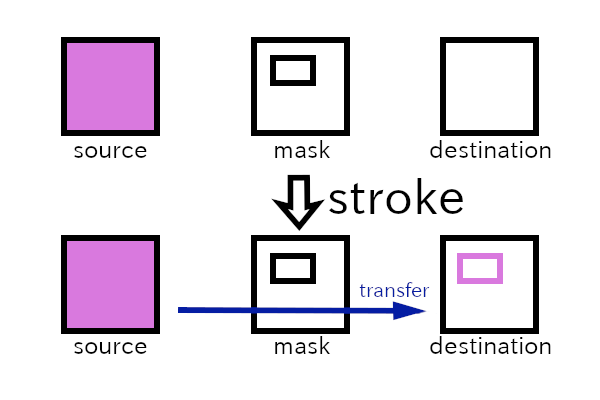
\includegraphics[width=9cm,height=6cm]{../image/cairo.png}
\caption{Stroke a rectangle}
\end{figure}

The instruction is as follows:

\begin{enumerate}
\def\labelenumi{\arabic{enumi}.}
\tightlist
\item
  Create a surface. This will be the destination.
\item
  Create a cairo context with the surface, the surface will be the
  destination of the context.
\item
  Create a source pattern within the context.
\item
  Create paths, which are lines, rectangles, arcs, texts or more
  complicated shapes in the mask.
\item
  Use a drawing operator such as \passthrough{\lstinline!cairo\_stroke!}
  to transfer the paint in the source to the destination.
\item
  Save the destination surface to a file if necessary.
\end{enumerate}

Here's a simple example program that draws a small square and saves it
as a png file.

\begin{lstlisting}[language=C, numbers=left]
#include <cairo.h>

int
main (int argc, char **argv)
{
  cairo_surface_t *surface;
  cairo_t *cr;
  int width = 100;
  int height = 100;
  int square_size = 40.0;

  /* Create surface and cairo */
  surface = cairo_image_surface_create (CAIRO_FORMAT_RGB24, width, height);
  cr = cairo_create (surface);

  /* Drawing starts here. */
  /* Paint the background white */
  cairo_set_source_rgb (cr, 1.0, 1.0, 1.0);
  cairo_paint (cr);
  /* Draw a black rectangle */
  cairo_set_source_rgb (cr, 0.0, 0.0, 0.0);
  cairo_set_line_width (cr, 2.0);
  cairo_rectangle (cr,
                   width/2.0 - square_size/2,
                   height/2.0 - square_size/2,
                   square_size,
                   square_size);
  cairo_stroke (cr);

  /* Write the surface to a png file and clean up cairo and surface. */
  cairo_surface_write_to_png (surface, "rectangle.png");
  cairo_destroy (cr);
  cairo_surface_destroy (surface);

  return 0;
}
\end{lstlisting}

\begin{itemize}
\tightlist
\item
  1: Includes the header file of Cairo.
\item
  6: \passthrough{\lstinline!cairo\_surface\_t!} is the type of a
  surface.
\item
  7: \passthrough{\lstinline!cairo\_t!} is the type of a cairo context.
\item
  8-10: \passthrough{\lstinline!width!} and
  \passthrough{\lstinline!height!} are the size of
  \passthrough{\lstinline!surface!}.
  \passthrough{\lstinline!square\_size!} is the size of a square to be
  drawn on the surface.
\item
  13: \passthrough{\lstinline!cairo\_image\_surface\_create!} creates an
  image surface. \passthrough{\lstinline!CAIRO\_FORMAT\_RGB24!} is a
  constant which means that each pixel has red, green and blue data, and
  each data point is an 8 bits number (for 24 bits in total). Modern
  displays have this type of color depth. Width and height are in pixels
  and given as integers.
\item
  14: Creates cairo context. The surface given as an argument will be
  the destination of the context.
\item
  18: \passthrough{\lstinline!cairo\_set\_source\_rgb!} creates a source
  pattern, which in this case is a solid white paint. The second to
  fourth argument are red, green and blue color values respectively, and
  they are of type float. The values are between zero (0.0) and one
  (1.0), with black being given by (0.0,0.0,0.0) and white by
  (1.0,1.0,1.0).
\item
  19: \passthrough{\lstinline!cairo\_paint!} copies everywhere in the
  source to destination. The destination is filled with white pixels
  with this command.
\item
  21: Sets the source color to black.
\item
  22: \passthrough{\lstinline!cairo\_set\_line\_width!} set the width of
  lines. In this case, the line width is set to be two pixels and will
  end up that same size. (It is because the transformation is identity.
  If the transformation isn't identity, for example scaling with the
  factor three, the actual width in destination will be six (2x3=6)
  pixels.)
\item
  23: Draws a rectangle (square) on the mask. The square is located at
  the center.
\item
  24: \passthrough{\lstinline!cairo\_stroke!} transfer the source to
  destination through the rectangle in the mask.
\item
  27: Outputs the image to a png file
  \passthrough{\lstinline!rectangle.png!}.
\item
  28: Destroys the context. At the same time the source is destroyed.
\item
  29: Destroys the surface.
\end{itemize}

To compile this, type the following.

\begin{lstlisting}
$ gcc `pkg-config --cflags cairo` cairo.c `pkg-config --libs cairo`
\end{lstlisting}

\begin{figure}
\centering
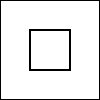
\includegraphics{../image/rectangle.png}
\caption{rectangle.png}
\end{figure}

See the \href{https://www.cairographics.org/}{Cairo's website} for more
details.

\hypertarget{gtkdrawingarea}{%
\subsection{GtkDrawingArea}\label{gtkdrawingarea}}

The following is a very simple example.

\begin{lstlisting}[language=C, numbers=left]
#include <gtk/gtk.h>

static void
draw_function (GtkDrawingArea *area, cairo_t *cr, int width, int height, gpointer user_data) {
  int square_size = 40.0;

  cairo_set_source_rgb (cr, 1.0, 1.0, 1.0); /* white */
  cairo_paint (cr);
  cairo_set_line_width (cr, 2.0);
  cairo_set_source_rgb (cr, 0.0, 0.0, 0.0); /* black */
  cairo_rectangle (cr,
                   width/2.0 - square_size/2,
                   height/2.0 - square_size/2,
                   square_size,
                   square_size);
  cairo_stroke (cr);
}

static void
app_activate (GApplication *app, gpointer user_data) {
  GtkWidget *win = gtk_application_window_new (GTK_APPLICATION (app));
  GtkWidget *area = gtk_drawing_area_new ();

  gtk_window_set_title (GTK_WINDOW (win), "da1");
  gtk_drawing_area_set_draw_func (GTK_DRAWING_AREA (area), draw_function, NULL, NULL);
  gtk_window_set_child (GTK_WINDOW (win), area);

  gtk_widget_show (win);
}

#define APPLICATION_ID "com.github.ToshioCP.da1"

int
main (int argc, char **argv) {
  GtkApplication *app;
  int stat;

  app = gtk_application_new (APPLICATION_ID, G_APPLICATION_FLAGS_NONE);
  g_signal_connect (app, "activate", G_CALLBACK (app_activate), NULL);
  stat =g_application_run (G_APPLICATION (app), argc, argv);
  g_object_unref (app);
  return stat;
}
\end{lstlisting}

The function \passthrough{\lstinline!main!} is almost same as before.
The two functions \passthrough{\lstinline!app\_activate!} and
\passthrough{\lstinline!draw\_function!} are important in this example.

\begin{itemize}
\tightlist
\item
  18: Creates a GtkDrawingArea instance; and
\item
  21: Sets a drawing function of the widget. GtkDrawingArea widget uses
  the function to draw the contents of itself whenever its necessary.
  For example, when a user drag a mouse pointer and resize a top-level
  window, GtkDrawingArea also changes the size. Then, the whole window
  needs to be redrawn. For the information of
  \passthrough{\lstinline!gtk\_drawing\_area\_set\_draw\_func!}, see
  \href{https://docs.gtk.org/gtk4/method.DrawingArea.set_draw_func.html}{Gtk
  API Reference, gtk\_drawing\_area\_set\_draw\_func}.
\end{itemize}

The drawing function has five parameters.

\begin{lstlisting}[language=C]
void drawing_function (GtkDrawingArea *drawing_area, cairo_t *cr, int width, int height,
                       gpointer user_data);
\end{lstlisting}

The first parameter is the GtkDrawingArea widget. You can't change any
properties, for example \passthrough{\lstinline!content-width!} or
\passthrough{\lstinline!content-height!}, in this function. The second
parameter is a cairo context given by the widget. The destination
surface of the context is connected to the contents of the widget. What
you draw to this surface will appear in the widget on the screen. The
third and fourth parameters are the size of the destination surface.
Now, look at the program example again.

\begin{itemize}
\tightlist
\item
  3-13: The drawing function.
\item
  7-8: Sets the source to be white and paint the destination white.
\item
  9: Sets the line width to be 2.
\item
  10: Sets the source to be black.
\item
  11: Adds a rectangle to the mask.
\item
  12: Draws the rectangle with black color to the destination.
\end{itemize}

Compile and run it, then a window with a black rectangle (square)
appears. Try resizing the window. The square always appears at the
center of the window because the drawing function is invoked each time
the window is resized.

\begin{figure}
\centering
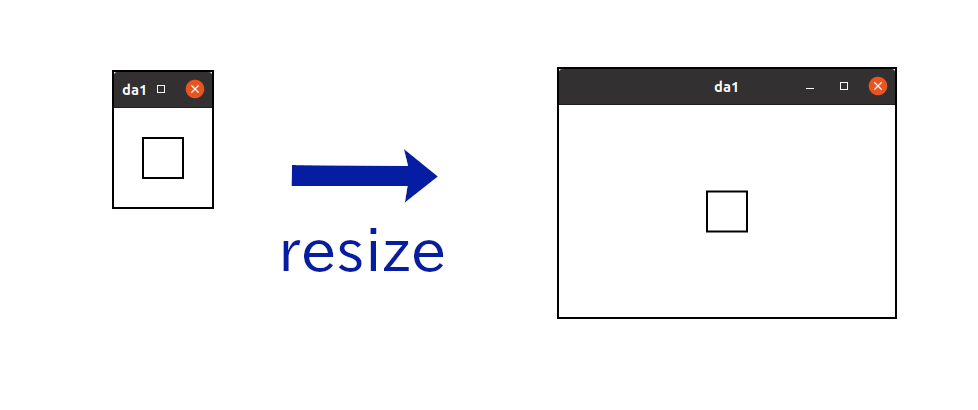
\includegraphics[width=8cm,height=3.4cm]{../image/da1.png}
\caption{Square in the window}
\end{figure}

  \hypertarget{periodic-events}{%
\section{Periodic Events}\label{periodic-events}}

This chapter was written by Paul Schulz
\href{mailto:paul@mawsonlakes.org}{\nolinkurl{paul@mawsonlakes.org}}.

\hypertarget{how-do-we-create-an-animation}{%
\subsection{How do we create an
animation?}\label{how-do-we-create-an-animation}}

In this section we will continue to build on our previous work. We will
create an analog clock application. By adding a function which
periodically redraws GtkDrawingArea, the clock will be able to
continuously display the time.

The application uses a compiled in `resource' file, so if the GTK4
libraries and their dependencies are installed and available, the
application will run from anywhere.

The program also makes use of some standard mathematical and time
handling functions.

The clocks mechanics were taken from a Cairo drawing example, using
gtkmm4, which can be found
\href{https://developer-old.gnome.org/gtkmm-tutorial/stable/sec-drawing-clock-example.html.en}{here}.

The complete code is at the end.

\hypertarget{drawing-the-clock-face-hour-minute-and-second-hands}{%
\subsection{Drawing the clock face, hour, minute and second
hands}\label{drawing-the-clock-face-hour-minute-and-second-hands}}

The \passthrough{\lstinline!draw\_clock()!} function does all the work.
See the in-file comments for an explanation of how the Cairo drawing
works.

For a detailed reference of what each of the Cairo functions does see
the
\href{https://www.cairographics.org/manual/cairo-cairo-t.html}{cairo\_t
reference}.

\begin{lstlisting}[language=C, numbers=left]
static void
draw_clock (GtkDrawingArea *area, cairo_t *cr, int width, int height, gpointer user_data) {

    // Scale to unit square and translate (0, 0) to be (0.5, 0.5), i.e.
    // the center of the window
    cairo_scale(cr, width, height);
    cairo_translate(cr, 0.5, 0.5);

    // Set the line width and save the cairo drawing state.
    cairo_set_line_width(cr, m_line_width);
    cairo_save(cr);

    // Set the background to a slightly transparent green.
    cairo_set_source_rgba(cr, 0.337, 0.612, 0.117, 0.9);   // green
    cairo_paint(cr);

    // Resore back to precious drawing state and draw the circular path
    // representing the clockface. Save this state (including the path) so we
    // can reuse it.
    cairo_restore(cr);
    cairo_arc(cr, 0.0, 0.0, m_radius, 0.0, 2.0 * M_PI);
    cairo_save(cr);

    // Fill the clockface with white
    cairo_set_source_rgba(cr, 1.0, 1.0, 1.0, 0.8);
    cairo_fill_preserve(cr);
    // Restore the path, paint the outside of the clock face.
    cairo_restore(cr);
    cairo_stroke_preserve(cr);
    // Set the 'clip region' to the inside of the path (fill region).
    cairo_clip(cr);

    // Clock ticks
    for (int i = 0; i < 12; i++)
    {
        // Major tick size
        double inset = 0.05;

        // Save the graphics state, restore after drawing tick to maintain pen
        // size
        cairo_save(cr);
        cairo_set_line_cap(cr, CAIRO_LINE_CAP_ROUND);

        // Minor ticks are shorter, and narrower.
        if(i % 3 != 0)
        {
            inset *= 0.8;
            cairo_set_line_width(cr, 0.03);
        }

        // Draw tick mark
        cairo_move_to(
            cr,
            (m_radius - inset) * cos (i * M_PI / 6.0),
            (m_radius - inset) * sin (i * M_PI / 6.0));
        cairo_line_to(
            cr,
            m_radius * cos (i * M_PI / 6.0),
            m_radius * sin (i * M_PI / 6.0));
        cairo_stroke(cr);
        cairo_restore(cr); /* stack-pen-size */
    }

    // Draw the analog hands

    // Get the current Unix time, convert to the local time and break into time
    // structure to read various time parts.
    time_t rawtime;
    time(&rawtime);
    struct tm * timeinfo = localtime (&rawtime);

    // Calculate the angles of the hands of our clock
    double hours   = timeinfo->tm_hour * M_PI / 6.0;
    double minutes = timeinfo->tm_min * M_PI / 30.0;
    double seconds = timeinfo->tm_sec * M_PI / 30.0;

    // Save the graphics state
    cairo_save(cr);
    cairo_set_line_cap(cr, CAIRO_LINE_CAP_ROUND);

    cairo_save(cr);

    // Draw the seconds hand
    cairo_set_line_width(cr, m_line_width / 3.0);
    cairo_set_source_rgba(cr, 0.7, 0.7, 0.7, 0.8);   // gray
    cairo_move_to(cr, 0.0, 0.0);
    cairo_line_to(cr,
                  sin(seconds) * (m_radius * 0.9),
                  -cos(seconds) * (m_radius * 0.9));
    cairo_stroke(cr);
    cairo_restore(cr);

    // Draw the minutes hand
    cairo_set_source_rgba(cr, 0.117, 0.337, 0.612, 0.9);   // blue
    cairo_move_to(cr, 0, 0);
    cairo_line_to(cr,
                  sin(minutes + seconds / 60) * (m_radius * 0.8),
                  -cos(minutes + seconds / 60) * (m_radius * 0.8));
    cairo_stroke(cr);

    // draw the hours hand
    cairo_set_source_rgba(cr, 0.337, 0.612, 0.117, 0.9);   // green
    cairo_move_to(cr, 0.0, 0.0);
    cairo_line_to(cr,
                  sin(hours + minutes / 12.0) * (m_radius * 0.5),
                  -cos(hours + minutes / 12.0) * (m_radius * 0.5));
    cairo_stroke(cr);
    cairo_restore(cr);

    // Draw a little dot in the middle
    cairo_arc(cr, 0.0, 0.0, m_line_width / 3.0, 0.0, 2.0 * M_PI);
    cairo_fill(cr);
}
\end{lstlisting}

In order for the clock to be drawn, the drawing function
\passthrough{\lstinline!draw\_clock()!} needs to be registered with
GTK4. This is done in the \passthrough{\lstinline!app\_activate()!}
function (on line 24).

Whenever the application needs to redraw the GtkDrawingArea, it will now
call \passthrough{\lstinline!draw\_clock()!}.

There is still a problem though. In order to animate the clock we need
to also tell the application that the clock needs to be redrawn every
second. This process starts by registering (on the next line, line 15) a
timeout function with \passthrough{\lstinline!g\_timeout\_add()!} that
will wakeup and run another function
\passthrough{\lstinline!time\_handler!}, every second (or 1000ms).

\begin{lstlisting}[language=C, numbers=left]
static void
app_activate (GApplication *app, gpointer user_data) {
    GtkWidget *win;
    GtkWidget *clock;
    GtkBuilder *build;

    build = gtk_builder_new_from_resource ("/com/github/ToshioCP/tfc/tfc.ui");
    win = GTK_WIDGET (gtk_builder_get_object (build, "win"));
    gtk_window_set_application (GTK_WINDOW (win), GTK_APPLICATION (app));

    clock = GTK_WIDGET (gtk_builder_get_object (build, "clock"));
    g_object_unref(build);

    gtk_drawing_area_set_draw_func(GTK_DRAWING_AREA (clock), draw_clock, NULL, NULL);
    g_timeout_add(1000, (GSourceFunc) time_handler, (gpointer) clock);
    gtk_widget_show(win);

}
\end{lstlisting}

Our \passthrough{\lstinline!time\_handler()!} function is very simple,
as it just calls \passthrough{\lstinline!gtk\_widget\_queue\_draw()!}
which schedules a redraw of the widget.

\begin{lstlisting}[language=C, numbers=left]
gboolean
time_handler(GtkWidget* widget) {
    gtk_widget_queue_draw(widget);

    return TRUE;
}
\end{lstlisting}

.. and that is all there is to it. If you compile and run the example
you will get a ticking analog clock.

If you get this working, you can try modifying some of the code in
\passthrough{\lstinline!draw\_clock()!} to tweak the application (such
as change the color or size and length of the hands) or even add text,
or create a digital clock.

\hypertarget{the-complete-code}{%
\subsection{The Complete code}\label{the-complete-code}}

You can find the source files in the \passthrough{\lstinline!tfc!}
directory. it can be compiled with \passthrough{\lstinline!./comp tfc!}.

\passthrough{\lstinline!tfc.c!}

\begin{lstlisting}[language=C, numbers=left]
#include <gtk/gtk.h>
#include <math.h>
#include <time.h>

float m_radius     = 0.42;
float m_line_width = 0.05;

static void
draw_clock (GtkDrawingArea *area, cairo_t *cr, int width, int height, gpointer user_data) {

    // Scale to unit square and translate (0, 0) to be (0.5, 0.5), i.e.
    // the center of the window
    cairo_scale(cr, width, height);
    cairo_translate(cr, 0.5, 0.5);

    // Set the line width and save the cairo drawing state.
    cairo_set_line_width(cr, m_line_width);
    cairo_save(cr);

    // Set the background to a slightly transparent green.
    cairo_set_source_rgba(cr, 0.337, 0.612, 0.117, 0.9);   // green
    cairo_paint(cr);

    // Resore back to precious drawing state and draw the circular path
    // representing the clockface. Save this state (including the path) so we
    // can reuse it.
    cairo_restore(cr);
    cairo_arc(cr, 0.0, 0.0, m_radius, 0.0, 2.0 * M_PI);
    cairo_save(cr);

    // Fill the clockface with white
    cairo_set_source_rgba(cr, 1.0, 1.0, 1.0, 0.8);
    cairo_fill_preserve(cr);
    // Restore the path, paint the outside of the clock face.
    cairo_restore(cr);
    cairo_stroke_preserve(cr);
    // Set the 'clip region' to the inside of the path (fill region).
    cairo_clip(cr);

    // Clock ticks
    for (int i = 0; i < 12; i++)
    {
        // Major tick size
        double inset = 0.05;

        // Save the graphics state, restore after drawing tick to maintain pen
        // size
        cairo_save(cr);
        cairo_set_line_cap(cr, CAIRO_LINE_CAP_ROUND);

        // Minor ticks are shorter, and narrower.
        if(i % 3 != 0)
        {
            inset *= 0.8;
            cairo_set_line_width(cr, 0.03);
        }

        // Draw tick mark
        cairo_move_to(
            cr,
            (m_radius - inset) * cos (i * M_PI / 6.0),
            (m_radius - inset) * sin (i * M_PI / 6.0));
        cairo_line_to(
            cr,
            m_radius * cos (i * M_PI / 6.0),
            m_radius * sin (i * M_PI / 6.0));
        cairo_stroke(cr);
        cairo_restore(cr); /* stack-pen-size */
    }

    // Draw the analog hands

    // Get the current Unix time, convert to the local time and break into time
    // structure to read various time parts.
    time_t rawtime;
    time(&rawtime);
    struct tm * timeinfo = localtime (&rawtime);

    // Calculate the angles of the hands of our clock
    double hours   = timeinfo->tm_hour * M_PI / 6.0;
    double minutes = timeinfo->tm_min * M_PI / 30.0;
    double seconds = timeinfo->tm_sec * M_PI / 30.0;

    // Save the graphics state
    cairo_save(cr);
    cairo_set_line_cap(cr, CAIRO_LINE_CAP_ROUND);

    cairo_save(cr);

    // Draw the seconds hand
    cairo_set_line_width(cr, m_line_width / 3.0);
    cairo_set_source_rgba(cr, 0.7, 0.7, 0.7, 0.8);   // gray
    cairo_move_to(cr, 0.0, 0.0);
    cairo_line_to(cr,
                  sin(seconds) * (m_radius * 0.9),
                  -cos(seconds) * (m_radius * 0.9));
    cairo_stroke(cr);
    cairo_restore(cr);

    // Draw the minutes hand
    cairo_set_source_rgba(cr, 0.117, 0.337, 0.612, 0.9);   // blue
    cairo_move_to(cr, 0, 0);
    cairo_line_to(cr,
                  sin(minutes + seconds / 60) * (m_radius * 0.8),
                  -cos(minutes + seconds / 60) * (m_radius * 0.8));
    cairo_stroke(cr);

    // draw the hours hand
    cairo_set_source_rgba(cr, 0.337, 0.612, 0.117, 0.9);   // green
    cairo_move_to(cr, 0.0, 0.0);
    cairo_line_to(cr,
                  sin(hours + minutes / 12.0) * (m_radius * 0.5),
                  -cos(hours + minutes / 12.0) * (m_radius * 0.5));
    cairo_stroke(cr);
    cairo_restore(cr);

    // Draw a little dot in the middle
    cairo_arc(cr, 0.0, 0.0, m_line_width / 3.0, 0.0, 2.0 * M_PI);
    cairo_fill(cr);
}


gboolean
time_handler(GtkWidget* widget) {
    gtk_widget_queue_draw(widget);

    return TRUE;
}


static void
app_activate (GApplication *app, gpointer user_data) {
    GtkWidget *win;
    GtkWidget *clock;
    GtkBuilder *build;

    build = gtk_builder_new_from_resource ("/com/github/ToshioCP/tfc/tfc.ui");
    win = GTK_WIDGET (gtk_builder_get_object (build, "win"));
    gtk_window_set_application (GTK_WINDOW (win), GTK_APPLICATION (app));

    clock = GTK_WIDGET (gtk_builder_get_object (build, "clock"));
    g_object_unref(build);

    gtk_drawing_area_set_draw_func(GTK_DRAWING_AREA (clock), draw_clock, NULL, NULL);
    g_timeout_add(1000, (GSourceFunc) time_handler, (gpointer) clock);
    gtk_widget_show(win);

}

static void
app_open (GApplication *app, GFile **files, gint n_files, gchar *hint, gpointer user_data) {
    app_activate(app,user_data);
}

int
main (int argc, char **argv) {
    GtkApplication *app;
    int stat;

    app = gtk_application_new ("com.github.ToshioCP.tfc", G_APPLICATION_HANDLES_OPEN);
    g_signal_connect (app, "activate", G_CALLBACK (app_activate), NULL);
    g_signal_connect (app, "open", G_CALLBACK (app_open), NULL);
    stat = g_application_run (G_APPLICATION (app), argc, argv);
    g_object_unref (app);
    return stat;
}
\end{lstlisting}

\passthrough{\lstinline!tfc.ui!}

\begin{lstlisting}[language=XML, numbers=left]
<?xml version="1.0" encoding="UTF-8"?>
<interface>
  <object class="GtkApplicationWindow" id="win">
    <property name="title">Clock</property>
    <property name="default-width">200</property>
    <property name="default-height">200</property>
    <child>
      <object class="GtkDrawingArea" id="clock">
        <property name="hexpand">TRUE</property>
        <property name="vexpand">TRUE</property>
      </object>
    </child>
  </object>
</interface>
\end{lstlisting}

\passthrough{\lstinline!tfc.gresource.xml!}

\begin{lstlisting}[language=XML, numbers=left]
<?xml version="1.0" encoding="UTF-8"?>
<gresources>
  <gresource prefix="/com/github/ToshioCP/tfc">
    <file>tfc.ui</file>
  </gresource>
</gresources>
\end{lstlisting}

\passthrough{\lstinline!comp!}

\begin{lstlisting}[numbers=left]
glib-compile-resources $1.gresource.xml --target=$1.gresource.c --generate-source
gcc `pkg-config --cflags gtk4` $1.gresource.c $1.c `pkg-config --libs gtk4` -lm
\end{lstlisting}

  \hypertarget{combine-gtkdrawingarea-and-tfetextview}{%
\section{Combine GtkDrawingArea and
TfeTextView}\label{combine-gtkdrawingarea-and-tfetextview}}

Now, we will make a new application which has GtkDrawingArea and
TfeTextView in it. Its name is ``color''. If you write a name of a color
in TfeTextView and click on the \passthrough{\lstinline!run!} button,
then the color of GtkDrawingArea changes to the color given by you.

\begin{figure}
\centering
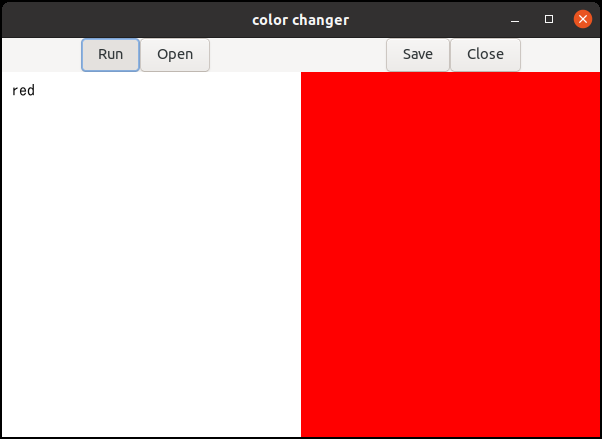
\includegraphics[width=7cm,height=5.13cm]{../image/color.png}
\caption{color}
\end{figure}

The following colors are available.

\begin{itemize}
\tightlist
\item
  white
\item
  black
\item
  red
\item
  green
\item
  blue
\end{itemize}

In addition the following two options are also available.

\begin{itemize}
\tightlist
\item
  light: Make the color of the drawing area lighter.
\item
  dark: Make the color of the drawing area darker.
\end{itemize}

This application can only do very simple things. However, it tells us
that if we add powerful parser to it, we will be able to make it more
efficient. I want to show it to you in the later section by making a
turtle graphics language like Logo program language.

In this section, we focus on how to bind the two objects.

\hypertarget{color.ui-and-color.gresource.xml}{%
\subsection{Color.ui and
color.gresource.xml}\label{color.ui-and-color.gresource.xml}}

First, We need to make the ui file of the widgets. The image in the
previous subsection gives us the structure of the widgets. Title bar,
four buttons in the tool bar and two widgets textview and drawing area.
The ui file is as follows.

\begin{lstlisting}[language=XML, numbers=left]
<?xml version="1.0" encoding="UTF-8"?>
<interface>
  <object class="GtkApplicationWindow" id="win">
    <property name="title">color changer</property>
    <property name="default-width">600</property>
    <property name="default-height">400</property>
    <child>
      <object class="GtkBox" id="boxv">
        <property name="orientation">GTK_ORIENTATION_VERTICAL</property>
        <child>
          <object class="GtkBox" id="boxh1">
            <property name="orientation">GTK_ORIENTATION_HORIZONTAL</property>
            <child>
              <object class="GtkLabel" id="dmy1">
                <property name="width-chars">10</property>
              </object>
            </child>
            <child>
              <object class="GtkButton" id="btnr">
                <property name="label">Run</property>
                <signal name="clicked" handler="run_cb"></signal>
              </object>
            </child>
            <child>
              <object class="GtkButton" id="btno">
                <property name="label">Open</property>
                <signal name="clicked" handler="open_cb"></signal>
              </object>
            </child>
            <child>
              <object class="GtkLabel" id="dmy2">
                <property name="hexpand">TRUE</property>
              </object>
            </child>
            <child>
              <object class="GtkButton" id="btns">
                <property name="label">Save</property>
                <signal name="clicked" handler="save_cb"></signal>
              </object>
            </child>
            <child>
              <object class="GtkButton" id="btnc">
                <property name="label">Close</property>
                <signal name="clicked" handler="close_cb"></signal>
              </object>
            </child>
            <child>
              <object class="GtkLabel" id="dmy3">
                <property name="width-chars">10</property>
              </object>
            </child>
          </object>
        </child>
        <child>
          <object class="GtkBox" id="boxh2">
            <property name="orientation">GTK_ORIENTATION_HORIZONTAL</property>
            <property name="homogeneous">TRUE</property>
            <child>
              <object class="GtkScrolledWindow" id="scr">
                <property name="hexpand">TRUE</property>
                <property name="vexpand">TRUE</property>
                <child>
                  <object class="TfeTextView" id="tv">
                    <property name="wrap-mode">GTK_WRAP_WORD_CHAR</property>
                  </object>
                </child>
              </object>
            </child>
            <child>
              <object class="GtkDrawingArea" id="da">
                <property name="hexpand">TRUE</property>
                <property name="vexpand">TRUE</property>
              </object>
            </child>
          </object>
        </child>
      </object>
    </child>
  </object>
</interface>
\end{lstlisting}

\begin{itemize}
\tightlist
\item
  10-53: This part is the tool bar which has four buttons,
  \passthrough{\lstinline!Run!}, \passthrough{\lstinline!Open!},
  \passthrough{\lstinline!Save!} and \passthrough{\lstinline!Close!}.
  This is similar to the toolbar of tfe text editor in Section 9. There
  are two differences. \passthrough{\lstinline!Run!} button replaces
  \passthrough{\lstinline!New!} button. A signal element is added to
  each button object. It has ``name'' attribute which is a signal name
  and ``handler'' attribute which is the name of its signal handler
  function. Options ``-WI, --export-dynamic'' CFLAG is necessary when
  you compile the application. You can achieve this by adding
  ``export\_dynamic: true'' argument to executable function in
  \passthrough{\lstinline!meson.build!}. And be careful that the handler
  must be defined without `static' class.
\item
  54-76: Puts GtkScrolledWindow and GtkDrawingArea into GtkBox. GtkBox
  has ``homogeneous property'' with TRUE value, so the two children have
  the same width in the box. TfeTextView is a child of
  GtkScrolledWindow.
\end{itemize}

The xml file for the resource compiler is almost same as before. Just
substitute ``color'' for ``tfe''.

\begin{lstlisting}[language=XML, numbers=left]
<?xml version="1.0" encoding="UTF-8"?>
<gresources>
  <gresource prefix="/com/github/ToshioCP/color">
    <file>color.ui</file>
  </gresource>
</gresources>
\end{lstlisting}

\hypertarget{tfetextview.h-tfetextview.c-and-color.h}{%
\subsection{Tfetextview.h, tfetextview.c and
color.h}\label{tfetextview.h-tfetextview.c-and-color.h}}

First two files are the same as before. Color.h just includes
tfetextview.h.

\begin{lstlisting}[language=C, numbers=left]
#include <gtk/gtk.h>

#include "../tfetextview/tfetextview.h"
\end{lstlisting}

\hypertarget{colorapplication.c}{%
\subsection{Colorapplication.c}\label{colorapplication.c}}

This is the main file. It deals with:

\begin{itemize}
\tightlist
\item
  Building widgets by GtkBuilder.
\item
  Setting a drawing function of GtkDrawingArea. And connecting a handler
  to ``resize'' signal on GtkDrawingArea.
\item
  Implementing each call back functions. Particularly,
  \passthrough{\lstinline!Run!} signal handler is the point in this
  program.
\end{itemize}

The following is \passthrough{\lstinline!colorapplication.c!}.

\begin{lstlisting}[language=C, numbers=left]
#include "color.h"

static GtkWidget *win;
static GtkWidget *tv;
static GtkWidget *da;

static cairo_surface_t *surface = NULL;

static void
run (void) {
  GtkTextBuffer *tb = gtk_text_view_get_buffer (GTK_TEXT_VIEW (tv));
  GtkTextIter start_iter;
  GtkTextIter end_iter;
  char *contents;
  cairo_t *cr;

  gtk_text_buffer_get_bounds (tb, &start_iter, &end_iter);
  contents = gtk_text_buffer_get_text (tb, &start_iter, &end_iter, FALSE);
  if (surface) {
    cr = cairo_create (surface);
    if (g_strcmp0 ("red", contents) == 0)
      cairo_set_source_rgb (cr, 1, 0, 0);
    else if (g_strcmp0 ("green", contents) == 0)
      cairo_set_source_rgb (cr, 0, 1, 0);
    else if (g_strcmp0 ("blue", contents) == 0)
      cairo_set_source_rgb (cr, 0, 0, 1);
    else if (g_strcmp0 ("white", contents) == 0)
      cairo_set_source_rgb (cr, 1, 1, 1);
    else if (g_strcmp0 ("black", contents) == 0)
      cairo_set_source_rgb (cr, 0, 0, 0);
    else if (g_strcmp0 ("light", contents) == 0)
      cairo_set_source_rgba (cr, 1, 1, 1, 0.5);
    else if (g_strcmp0 ("dark", contents) == 0)
      cairo_set_source_rgba (cr, 0, 0, 0, 0.5);
    else
      cairo_set_source_surface (cr, surface, 0, 0);
    cairo_paint (cr);
    cairo_destroy (cr);
  }
  g_free (contents);
}

void
run_cb (GtkWidget *btnr) {
  run ();
  gtk_widget_queue_draw (GTK_WIDGET (da));
}

void
open_cb (GtkWidget *btno) {
  tfe_text_view_open (TFE_TEXT_VIEW (tv), GTK_WINDOW (win));
}

void
save_cb (GtkWidget *btns) {
  tfe_text_view_save (TFE_TEXT_VIEW (tv));
}

void
close_cb (GtkWidget *btnc) {
  if (surface)
    cairo_surface_destroy (surface);
  gtk_window_destroy (GTK_WINDOW (win));
}

static void
resize_cb (GtkDrawingArea *drawing_area, int width, int height, gpointer user_data) {
  if (surface)
    cairo_surface_destroy (surface);
  surface = cairo_image_surface_create (CAIRO_FORMAT_ARGB32, width, height);
  run ();
}

static void
draw_func (GtkDrawingArea *drawing_area, cairo_t *cr, int width, int height, gpointer user_data) {
  if (surface) {
    cairo_set_source_surface (cr, surface, 0, 0);
    cairo_paint (cr);
  }
}

static void
app_activate (GApplication *application) {
  gtk_widget_show (win);
}

static void
app_startup (GApplication *application) {
  GtkApplication *app = GTK_APPLICATION (application);
  GtkBuilder *build;

  build = gtk_builder_new_from_resource ("/com/github/ToshioCP/color/color.ui");
  win = GTK_WIDGET (gtk_builder_get_object (build, "win"));
  gtk_window_set_application (GTK_WINDOW (win), app);
  tv = GTK_WIDGET (gtk_builder_get_object (build, "tv"));
  da = GTK_WIDGET (gtk_builder_get_object (build, "da"));
  g_object_unref(build);
  g_signal_connect (GTK_DRAWING_AREA (da), "resize", G_CALLBACK (resize_cb), NULL);
  gtk_drawing_area_set_draw_func (GTK_DRAWING_AREA (da), draw_func, NULL, NULL);

GdkDisplay *display;

  display = gtk_widget_get_display (GTK_WIDGET (win));
  GtkCssProvider *provider = gtk_css_provider_new ();
  gtk_css_provider_load_from_data (provider, "textview {padding: 10px; font-family: monospace; font-size: 12pt;}", -1);
  gtk_style_context_add_provider_for_display (display, GTK_STYLE_PROVIDER (provider), GTK_STYLE_PROVIDER_PRIORITY_USER);
}

#define APPLICATION_ID "com.github.ToshioCP.color"

int
main (int argc, char **argv) {
  GtkApplication *app;
  int stat;

  app = gtk_application_new (APPLICATION_ID, G_APPLICATION_FLAGS_NONE);

  g_signal_connect (app, "startup", G_CALLBACK (app_startup), NULL);
  g_signal_connect (app, "activate", G_CALLBACK (app_activate), NULL);

  stat =g_application_run (G_APPLICATION (app), argc, argv);
  g_object_unref (app);
  return stat;
}
\end{lstlisting}

\begin{itemize}
\tightlist
\item
  109-124: The function \passthrough{\lstinline!main!} is almost same as
  before but there are some differences. The application ID is
  ``com.github.ToshioCP.color''.
  \passthrough{\lstinline!G\_APPLICATION\_FLAGS\_NONE!} is specified so
  no open signal handler is necessary.
\item
  87-107: Startup handler.
\item
  92-97: Builds widgets. The pointers of the top window, TfeTextView and
  GtkDrawingArea objects are stored to static variables
  \passthrough{\lstinline!win!}, \passthrough{\lstinline!tv!} and
  \passthrough{\lstinline!da!} respectively. This is because these
  objects are often used in handlers. They never be rewritten so they're
  thread safe.
\item
  98: connects ``resize'' signal and the handler.
\item
  99: sets the drawing function.
\item
  82-85: Activate handler, which just shows the widgets.
\item
  74-80: The drawing function. It just copies
  \passthrough{\lstinline!surface!} to destination.
\item
  66-72: Resize handler. Re-creates the surface to fit its width and
  height for the drawing area and paints by calling the function
  \passthrough{\lstinline!run!}.
\item
  59-64: Close handler. It destroys \passthrough{\lstinline!surface!} if
  it exists. Then it destroys the top-level window and quits the
  application.
\item
  49-57: Open and save handler. They just call the corresponding
  functions of TfeTextView.
\item
  43-47: Run handler. It calls run function to paint the surface. After
  that \passthrough{\lstinline!gtk\_widget\_queue\_draw!} is called.
  This function adds the widget (GtkDrawingArea) to the queue to be
  redrawn. It is important to know that the window is redrawn whenever
  it is necessary. For example, when another window is moved and
  uncovers part of the widget, or when the window containing it is
  resized. But repainting \passthrough{\lstinline!surface!} is not
  automatically notified to gtk. Therefore, you need to call
  \passthrough{\lstinline!gtk\_widget\_queue\_draw!} to redraw the
  widget.
\item
  9-41: Run function paints the surface. First, it gets the contents of
  GtkTextBuffer. Then it compares it to ``red'', ``green'' and so on. If
  it matches the color, then the surface is painted the color. If it
  matches ``light'' or ``dark'', then the color of the surface is
  lightened or darkened respectively. Alpha channel is used.
\end{itemize}

\hypertarget{meson.build}{%
\subsection{Meson.build}\label{meson.build}}

This file is almost same as before. An argument ``export\_dynamic:
true'' is added to executable function.

\begin{lstlisting}[numbers=left]
project('color', 'c')

gtkdep = dependency('gtk4')

gnome=import('gnome')
resources = gnome.compile_resources('resources','color.gresource.xml')

sourcefiles=files('colorapplication.c', '../tfetextview/tfetextview.c')

executable('color', sourcefiles, resources, dependencies: gtkdep, export_dynamic: true)
\end{lstlisting}

\hypertarget{compile-and-execute-it}{%
\subsection{Compile and execute it}\label{compile-and-execute-it}}

First you need to export some variables (refer to Section 2) if you've
installed Gtk4 from the source. If you've installed Gtk4 from the
distribution packages, you don't need to do this.

\begin{lstlisting}
$ . env.sh
\end{lstlisting}

Then type the following to compile it.

\begin{lstlisting}
$ meson _build
$ ninja -C _build
\end{lstlisting}

The application is made in \passthrough{\lstinline!\_build!} directory.
Type the following to execute it.

\begin{lstlisting}
$ _build/color
\end{lstlisting}

Type ``red'', ``green'', ``blue'', ``white'', black``,''light" or
``dark'' in the TfeTextView. Then, click on
\passthrough{\lstinline!Run!} button. Make sure the color of
GtkDrawingArea changes.

In this program TfeTextView is used to change the color. You can use
buttons or menus instead of textview. Probably it is more appropriate.
Using textview is unnatural. It is a good practice to make such
application by yourself.

  \hypertarget{tiny-turtle-graphics-interpreter}{%
\section{Tiny turtle graphics
interpreter}\label{tiny-turtle-graphics-interpreter}}

A program \passthrough{\lstinline!turtle!} is an example with the
combination of TfeTextView and GtkDrawingArea objects. It is a very
small interpreter but it provides a tool to draw fractal curves. The
following diagram is a Koch curve, which is a famous example of fractal
curves.

\begin{figure}
\centering
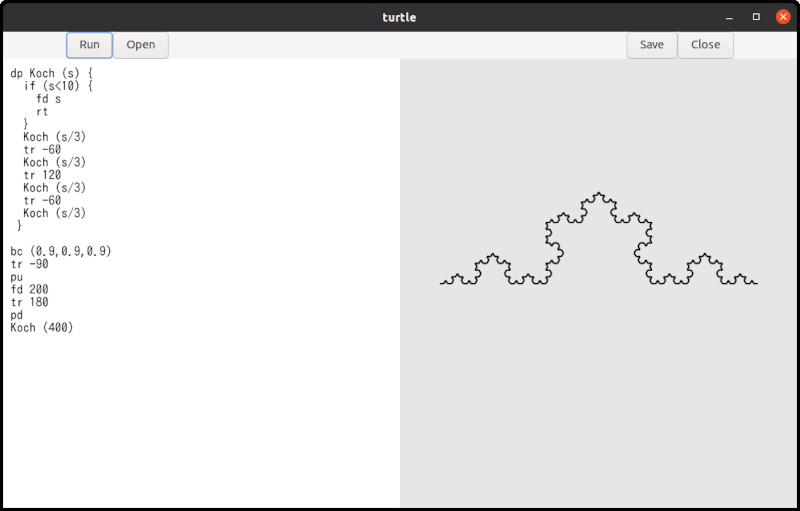
\includegraphics[width=8cm,height=5.11cm]{../src/turtle/image/turtle_koch.png}
\caption{Koch curve}
\end{figure}

This program uses flex and bison. Flex is a lexical analyzer. Bison is a
parser generator. These two programs are similar to lex and yacc which
are proprietary software developed in Bell Laboratory. However, flex and
bison are open source software. I will write about how to use those
software, but they are not topics about gtk. So, readers can skip that
part of this sections.

\hypertarget{how-to-use-turtle}{%
\subsection{How to use turtle}\label{how-to-use-turtle}}

The documentation of turtle is in the appendix. I'll show you a simple
example.

\begin{lstlisting}
fc (1,0,0) # Foreground color is red, rgb = (1,0,0).
pd         # Pen down.
fd 100     # Go forward by 100 pixels.
tr 90      # Turn right by 90 degrees.
fd 100
tr 90
fd 100
tr 90
fd 100
tr 90
\end{lstlisting}

\begin{enumerate}
\def\labelenumi{\arabic{enumi}.}
\tightlist
\item
  Compile and install \passthrough{\lstinline!turtle!} (See the
  documentation above). Then, run \passthrough{\lstinline!turtle!}.
\item
  Type the program above in the editor (left part of the window).
\item
  Click on the \passthrough{\lstinline!Run!} button, then a red square
  appears on the right part of the window. The side of the square is 100
  pixels long.
\end{enumerate}

In the same way, you can draw other curves. The documentation above
shows some fractal curves such as tree, snow and square-koch. The source
code in turtle language is located at src/turtle/example directory. You
can read these files into \passthrough{\lstinline!turtle!} editor by
clicking on the \passthrough{\lstinline!Open!} button.

\hypertarget{combination-of-tfetextview-and-gtkdrawingarea-objects}{%
\subsection{Combination of TfeTextView and GtkDrawingArea
objects}\label{combination-of-tfetextview-and-gtkdrawingarea-objects}}

Turtle uses TfeTextView and GtkDrawingArea. It is similar to
\passthrough{\lstinline!color!} program in the previous section.

\begin{enumerate}
\def\labelenumi{\arabic{enumi}.}
\tightlist
\item
  A user inputs/reads a turtle program into the buffer in the
  TfeTextView instance.
\item
  The user clicks on the ``Run'' button.
\item
  The parser reads the program and generates tree-structured data.
\item
  The interpriter reads the data and executes it step by step. And it
  draws shapes on a surface. The surface is different from the surface
  of the GtkDrawingArea widget.
\item
  The widget is added to the queue. It will be redrawn with the drawing
  function. The function just copies the surface, which is drawn by the
  interpreter, into the surface of the GtkDrawingArea.
\end{enumerate}

\begin{figure}
\centering
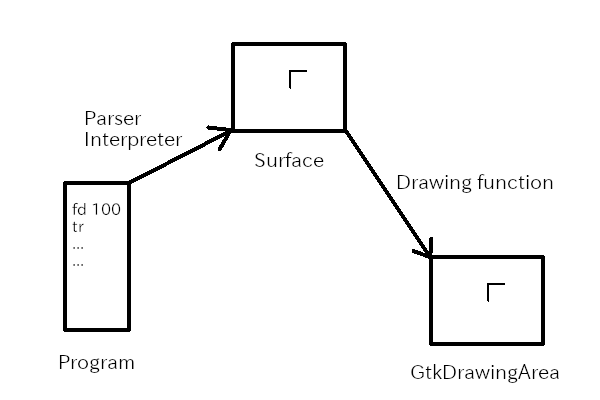
\includegraphics{../image/turtle.png}
\caption{Parser, interpreter and drawing function}
\end{figure}

The body of the interpreter is written with flex and bison. The codes
are not thread safe. So the handler of ``clicked'' signal of the
\passthrough{\lstinline!Run!} button prevents from reentering.

\begin{lstlisting}[language=C, numbers=left]
void
run_cb (GtkWidget *btnr) {
  GtkTextBuffer *tb = gtk_text_view_get_buffer (GTK_TEXT_VIEW (tv));
  GtkTextIter start_iter;
  GtkTextIter end_iter;
  char *contents;
  int stat;
  static gboolean busy = FALSE;

  /* yyparse() and run() are NOT thread safe. */
  /* The variable busy avoids reentry. */
  if (busy)
    return;
  busy = TRUE;
  gtk_text_buffer_get_bounds (tb, &start_iter, &end_iter);
  contents = gtk_text_buffer_get_text (tb, &start_iter, &end_iter, FALSE);
  if (surface) {
    init_flex (contents);
    stat = yyparse ();
    if (stat == 0) /* No error */ {
      run ();
    }
    finalize_flex ();
  }
  g_free (contents);
  gtk_widget_queue_draw (GTK_WIDGET (da));
  busy = FALSE;
}

static void
resize_cb (GtkDrawingArea *drawing_area, int width, int height, gpointer user_data) {
  if (surface)
    cairo_surface_destroy (surface);
  surface = cairo_image_surface_create (CAIRO_FORMAT_ARGB32, width, height);
}
\end{lstlisting}

\begin{itemize}
\tightlist
\item
  8-13: The static value \passthrough{\lstinline!busy!} holds a status
  of the interpreter. If it is \passthrough{\lstinline!TRUE!}, the
  interpreter is running and it is not possible to call the interpreter
  again because it's not a re-entrant program. If it is
  \passthrough{\lstinline!FALSE!}, it is safe to call the interpreter.
\item
  14: Now it is about to call the interpreter so it changes
  \passthrough{\lstinline!busy!} to TRUE.
\item
  15-16: Gets the contents of \passthrough{\lstinline!tb!}.
\item
  17: The variable \passthrough{\lstinline!surface!} is a static
  variable. It points to a \passthrough{\lstinline!cairo\_surface\_t!}
  instance. It is created when the GtkDrawingArea instance is realized
  and whenever it is resized. Therefore,
  \passthrough{\lstinline!surface!} isn't NULL usually. But if it is
  NULL, the interpreter won't be called.
\item
  18: Initializes lexical analyzer.
\item
  19: Calls parser. Parser analyzes the program codes syntactically and
  generate a tree structured data.
\item
  20-22: If the parser successfully parsed, it calls
  \passthrough{\lstinline!run!} (runtime routine).
\item
  23: finalizes the lexical analyzer.
\item
  25: frees \passthrough{\lstinline!contents!}.
\item
  26: Adds the drawing area widget to the queue to draw.
\item
  27: The interpreter program has finished so
  \passthrough{\lstinline!busy!} is now changed to FALSE.
\item
  29-34: A handler of ``resized'' signal. If
  \passthrough{\lstinline!surface!} isn't NULL, it destroys the old
  surface. Then it creates a new surface. Its size is the same as the
  surface of the GtkDrawingArea instance.
\end{itemize}

Other part of \passthrough{\lstinline!turtleapplication.c!} is almost
same as the codes of \passthrough{\lstinline!colorapplication.c!} in the
previous section. The codes of
\passthrough{\lstinline!turtleapplication.c!} is in the turtle
directory.

\hypertarget{what-does-the-interpreter-do}{%
\subsection{What does the interpreter
do?}\label{what-does-the-interpreter-do}}

Suppose that the turtle runs with the following program.

\begin{lstlisting}
distance = 100
fd distance*2
\end{lstlisting}

The turtle recognizes the program above and works as follows.

\begin{itemize}
\tightlist
\item
  Generally, a program consists of tokens. Tokens are ``distance'',
  ``='', ``100'', ``fd'', "*" and ``2'' in the above example..
\item
  The parser calls a function \passthrough{\lstinline!yylex!} to read a
  token in the source file. \passthrough{\lstinline!yylex!} returns a
  code which is called ``token kind'' and sets a global variable
  \passthrough{\lstinline!yylval!} with a value, which is called a
  semantic value. The type of \passthrough{\lstinline!yylval!} is union
  and \passthrough{\lstinline!yylval.ID!} is string and
  \passthrough{\lstinline!yylval.NUM!} is double. There are seven tokens
  in the program so \passthrough{\lstinline!yylex!} is called seven
  times.
\end{itemize}

\begin{longtable}[]{@{}cccc@{}}
\toprule
& token kind & yylval.ID & yylval.NUM\tabularnewline
\midrule
\endhead
1 & ID & distance &\tabularnewline
2 & = & &\tabularnewline
3 & NUM & & 100\tabularnewline
4 & FD & &\tabularnewline
5 & ID & distance &\tabularnewline
6 & * & &\tabularnewline
7 & NUM & & 2\tabularnewline
\bottomrule
\end{longtable}

\begin{itemize}
\tightlist
\item
  \passthrough{\lstinline!yylex!} returns a token kind every time, but
  it doesn't set \passthrough{\lstinline!yylval.ID!} or
  \passthrough{\lstinline!yylval.NUM!} every time. It is because
  keywords (\passthrough{\lstinline!FD!}) and symbols
  (\passthrough{\lstinline!=!} and \passthrough{\lstinline!*!}) don't
  have any semantic values. The function \passthrough{\lstinline!yylex!}
  is called lexical analyzer or scanner.
\item
  \passthrough{\lstinline!turtle!} makes a tree structured data. This
  part of \passthrough{\lstinline!turtle!} is called parser.
\end{itemize}

\begin{figure}
\centering
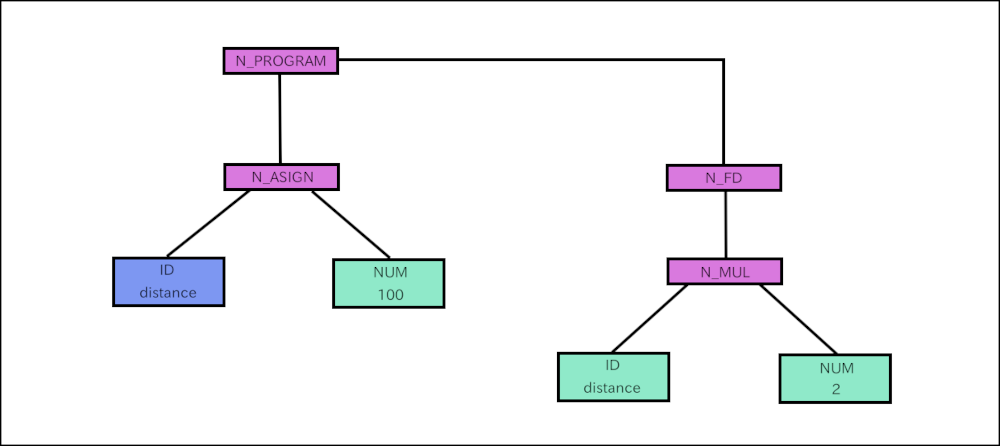
\includegraphics[width=12cm,height=5.34cm]{../image/turtle_parser_tree.png}
\caption{turtle parser tree}
\end{figure}

\begin{itemize}
\tightlist
\item
  \passthrough{\lstinline!turtle!} analyzes the tree and executes it.
  This part of \passthrough{\lstinline!turtle!} is called runtime
  routine or interpreter. The tree consists of rectangles and line
  segments between the rectangles. The rectangles are called nodes. For
  example, N\_PROGRAM, N\_ASSIGN, N\_FD and N\_MUL are nodes.

  \begin{enumerate}
  \def\labelenumi{\arabic{enumi}.}
  \tightlist
  \item
    Goes down from N\_PROGRAM to N\_ASSIGN.
  \item
    N\_ASSIGN node has two children, ID and NUM. This node comes from
    ``distance = 100'' which is ``ID = NUM'' syntactically. First,
    \passthrough{\lstinline!turtle!} checks if the first child is ID. If
    it's ID, then \passthrough{\lstinline!turtle!} looks for the
    variable in the variable table. If it doesn't exist, it registers
    the ID (\passthrough{\lstinline!distance!}) to the table. Then go
    back to the N\_ASSIGN node.
  \item
    \passthrough{\lstinline!turtle!} calculates the second child. In
    this case its a number 100. Saves 100 to the variable table at the
    \passthrough{\lstinline!distance!} record.
  \item
    \passthrough{\lstinline!turtle!} goes back to N\_PROGRAM then go to
    the next node N\_FD. It has only one child. Goes down to the child
    N\_MUL.
  \item
    The first child is ID (distance). Searches the variable table for
    the variable \passthrough{\lstinline!distance!} and gets the value
    100. The second child is a number 2. Multiplies 100 by 2 and gets
    200. Then \passthrough{\lstinline!turtle!} goes back to N\_FD.
  \item
    Now \passthrough{\lstinline!turtle!} knows the distance is 200. It
    moves the cursor forward by 200 pixels. The segment is drawn on the
    surface (\passthrough{\lstinline!surface!}).
  \item
    There are no node follows. Runtime routine returns to the function
    \passthrough{\lstinline!run\_cb!}.
  \end{enumerate}
\item
  \passthrough{\lstinline!run\_cb!} calls
  \passthrough{\lstinline!gtk\_widget\_queue\_draw!} and put the
  GtkDrawingArea widget to the queue.
\item
  The system redraws the widget. At that time drawing function
  \passthrough{\lstinline!draw\_func!} is called. The function copies
  the surface (\passthrough{\lstinline!surface!}) to the surface in the
  GtkDrawingArea.
\end{itemize}

Actual turtle program is more complicated than the example above.
However, what turtle does is basically the same. Interpretation consists
of three parts.

\begin{itemize}
\tightlist
\item
  Lexical analysis
\item
  Syntax Parsing and tree generation
\item
  Interpretation and execution of the tree.
\end{itemize}

\hypertarget{compilation-flow}{%
\subsection{Compilation flow}\label{compilation-flow}}

The source files are:

\begin{itemize}
\tightlist
\item
  flex source file =\textgreater{} \passthrough{\lstinline!turtle.lex!}
\item
  bison source file =\textgreater{} \passthrough{\lstinline!turtle.y!}
\item
  C header file =\textgreater{} \passthrough{\lstinline!turtle.h!},
  \passthrough{\lstinline!turtle\_lex.h!}
\item
  C source file =\textgreater{}
  \passthrough{\lstinline!turtleapplication.c!}
\item
  other files =\textgreater{} \passthrough{\lstinline!turtle.ui!},
  \passthrough{\lstinline!turtle.gresources.xml!} and
  \passthrough{\lstinline!meson.build!}
\end{itemize}

The compilation process is a bit complicated.

\begin{enumerate}
\def\labelenumi{\arabic{enumi}.}
\tightlist
\item
  glib-compile-resources compiles \passthrough{\lstinline!turtle.ui!} to
  \passthrough{\lstinline!resources.c!} according to
  \passthrough{\lstinline!turtle.gresource.xml!}. It also generates
  \passthrough{\lstinline!resources.h!}.
\item
  bison compiles \passthrough{\lstinline!turtle.y!} to
  \passthrough{\lstinline!turtle\_parser.c!} and generates
  \passthrough{\lstinline!turtle\_parser.h!}
\item
  flex compiles \passthrough{\lstinline!turtle.lex!} to
  \passthrough{\lstinline!turtle\_lex.c!}.
\item
  gcc compiles \passthrough{\lstinline!application.c!},
  \passthrough{\lstinline!resources.c!},
  \passthrough{\lstinline!turtle\_parser.c!} and
  \passthrough{\lstinline!turtle\_lex.c!} with
  \passthrough{\lstinline!turtle.h!},
  \passthrough{\lstinline!turtle\_lex.h!},
  \passthrough{\lstinline!resources.h!} and
  \passthrough{\lstinline!turtle\_parser.h!}. It generates an executable
  file \passthrough{\lstinline!turtle!}.
\end{enumerate}

\begin{figure}
\centering
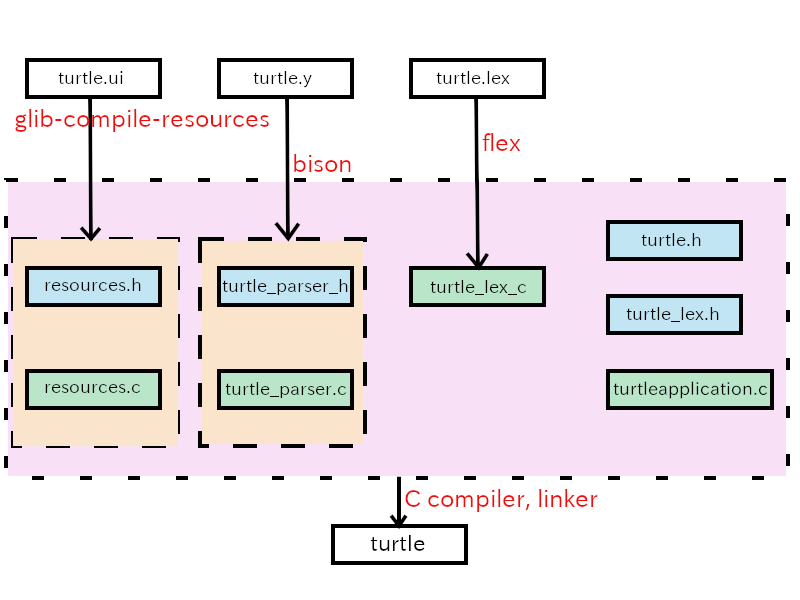
\includegraphics[width=12cm,height=9cm]{../image/turtle_compile_process.png}
\caption{compile process}
\end{figure}

Meson controls the process and the instruction is described in
\passthrough{\lstinline!meson.build!}.

\begin{lstlisting}[numbers=left]
project('turtle', 'c')

compiler = meson.get_compiler('c')
mathdep = compiler.find_library('m', required : true)

gtkdep = dependency('gtk4')

gnome=import('gnome')
resources = gnome.compile_resources('resources','turtle.gresource.xml')

flex = find_program('flex')
bison = find_program('bison')
turtleparser = custom_target('turtleparser', input: 'turtle.y', output: ['turtle_parser.c', 'turtle_parser.h'], command: [bison, '-d', '-o', 'turtle_parser.c', '@INPUT@'])
turtlelexer = custom_target('turtlelexer', input: 'turtle.lex', output: 'turtle_lex.c', command: [flex, '-o', '@OUTPUT@', '@INPUT@'])

sourcefiles=files('turtleapplication.c', '../tfetextview/tfetextview.c')

executable('turtle', sourcefiles, resources, turtleparser, turtlelexer, turtleparser[1], dependencies: [mathdep, gtkdep], export_dynamic: true, install: true)
\end{lstlisting}

\begin{itemize}
\tightlist
\item
  3: Gets C compiler. It is usually \passthrough{\lstinline!gcc!} in
  linux.
\item
  4: Gets math library. This program uses trigonometric functions. They
  are defined in the math library, but the library is optional. So, it
  is necessary to include it by
  \passthrough{\lstinline!\#include <math.h>!} and also link the library
  with the linker.
\item
  6: Gets gtk4 library.
\item
  8: Gets gnome module. Module is a system provided by meson. See
  \href{https://mesonbuild.com/Gnome-module.html\#gnome-module}{Meson
  build system website, GNUME module} for further information.
\item
  9: Compiles ui file to C source file according to the XML file
  \passthrough{\lstinline!turtle.gresource.xml!}.
\item
  11: Gets flex.
\item
  12: Gets bison.
\item
  13: Compiles \passthrough{\lstinline!turtle.y!} to
  \passthrough{\lstinline!turtle\_parser.c!} and
  \passthrough{\lstinline!turtle\_parser.h!} by bison. The function
  \passthrough{\lstinline!custom\_target!} creates a custom top level
  target. See
  \href{https://mesonbuild.com/Reference-manual.html\#custom_target}{Meson
  build system website, custom target} for further information.
\item
  14: Compiles \passthrough{\lstinline!turtle.lex!} to
  \passthrough{\lstinline!turtle\_lex.c!} by flex.
\item
  16: Specifies C source files.
\item
  18: Compiles C source files including generated files by
  glib-compile-resources, bison and flex. The argument
  \passthrough{\lstinline!turtleparser[1]!} refers to
  \passthrough{\lstinline!tirtle\_parser.h!} which is the second output
  in the line 13.
\end{itemize}

\hypertarget{turtle.lex}{%
\subsection{Turtle.lex}\label{turtle.lex}}

\hypertarget{what-does-flex-do}{%
\subsubsection{What does flex do?}\label{what-does-flex-do}}

Flex creates lexical analyzer from flex source file. Flex source file is
a text file. Its syntactic rule will be explained later. Generated
lexical analyzer is a C source file. It is also called scanner. It reads
a text file, which is a source file of a program language, and gets
variable names, numbers and symbols. Suppose here is a turtle source
file.

\begin{lstlisting}
fc (1,0,0) # Foreground color is red, rgb = (1,0,0).
pd         # Pen down.
distance = 100
angle = 90
fd distance    # Go forward by distance (100) pixels.
tr angle     # Turn right by angle (90) degrees.
\end{lstlisting}

The content of the text file is separated into
\passthrough{\lstinline!fc!}, \passthrough{\lstinline!(!},
\passthrough{\lstinline!1!} and so on. The words
\passthrough{\lstinline!fc!}, \passthrough{\lstinline!pd!},
\passthrough{\lstinline!distance!}, \passthrough{\lstinline!angle!},
\passthrough{\lstinline!tr!}, \passthrough{\lstinline!1!},
\passthrough{\lstinline!0!}, \passthrough{\lstinline!100!} and
\passthrough{\lstinline!90!} are called tokens. The characters
`\passthrough{\lstinline!(!}' (left parenthesis),
`\passthrough{\lstinline!,!}' (comma), `\passthrough{\lstinline!)!}'
(right parenthesis) and `\passthrough{\lstinline!=!}' (equal sign) are
called symbols. ( Sometimes those symbols called tokens, too.)

Flex reads \passthrough{\lstinline!turtle.lex!} and generates the C
source file of a scanner. The file \passthrough{\lstinline!turtle.lex!}
specifies tokens, symbols and the behavior which corresponds to each
token or symbol. Turtle.lex isn't a big program.

\begin{lstlisting}[numbers=left]
%top{
#include <string.h>
#include <stdlib.h>
#include "turtle.h"

  static int nline = 1;
  static int ncolumn = 1;
  static void get_location (char *text);

  /* Dinamically allocated memories are added to the single list. They will be freed in the finalize function. */
  extern GSList *list;
}

%option noyywrap

REAL_NUMBER (0|[1-9][0-9]*)(\.[0-9]+)?
IDENTIFIER [a-zA-Z][a-zA-Z0-9]*
%%
  /* rules */
#.*               ; /* comment. Be careful. Dot symbol (.) matches any character but new line. */
[ ]               ncolumn++;
\t                ncolumn += 8; /* assume that tab is 8 spaces. */
\n                nline++; ncolumn = 1;
  /* reserved keywords */
pu                get_location (yytext); return PU; /* pen up */
pd                get_location (yytext); return PD; /* pen down */
pw                get_location (yytext); return PW; /* pen width = line width */
fd                get_location (yytext); return FD; /* forward */
tr                get_location (yytext); return TR; /* turn right */
bc                get_location (yytext); return BC; /* background color */
fc                get_location (yytext); return FC; /* foreground color */
dp                get_location (yytext); return DP; /* define procedure */
if                get_location (yytext); return IF; /* if statement */
rt                get_location (yytext); return RT; /* return statement */
rs                get_location (yytext); return RS; /* reset the status */
  /* constant */
{REAL_NUMBER}     get_location (yytext); yylval.NUM = atof (yytext); return NUM;
  /* identifier */
{IDENTIFIER}      { get_location (yytext); yylval.ID = g_strdup(yytext);
                    list = g_slist_prepend (list, yylval.ID);
                    return ID;
                  }
"="               get_location (yytext); return '=';
">"               get_location (yytext); return '>';
"<"               get_location (yytext); return '<';
"+"               get_location (yytext); return '+';
"-"               get_location (yytext); return '-';
"*"               get_location (yytext); return '*';
"/"               get_location (yytext); return '/';
"("               get_location (yytext); return '(';
")"               get_location (yytext); return ')';
"{"               get_location (yytext); return '{';
"}"               get_location (yytext); return '}';
","               get_location (yytext); return ',';
.                 ncolumn++;             return YYUNDEF;
%%

static void
get_location (char *text) {
  yylloc.first_line = yylloc.last_line = nline;
  yylloc.first_column = ncolumn;
  yylloc.last_column = (ncolumn += strlen(text)) - 1;
}

static YY_BUFFER_STATE state;

void
init_flex (const char *text) {
  state = yy_scan_string (text);
}

void
finalize_flex (void) {
  yy_delete_buffer (state);
}
\end{lstlisting}

The file consists of three sections which are separated by ``\%\%''
(line 18 and 56). They are definitions, rules and user code sections.

\hypertarget{definitions-section}{%
\subsubsection{Definitions section}\label{definitions-section}}

\begin{itemize}
\tightlist
\item
  1-12: Lines between ``\%top\{'' and ``\}'' are C source codes. They
  will be copied to the top of the generated C source file.
\item
  2-3: The function \passthrough{\lstinline!strlen!}, in line 62, is
  defined in \passthrough{\lstinline!string.h!} The function
  \passthrough{\lstinline!atof!}, in line 37, is defined in
  \passthrough{\lstinline!stdlib.h!}.
\item
  6-8: The current input position is pointed by
  \passthrough{\lstinline!nline!} and \passthrough{\lstinline!ncolumn!}.
  The function \passthrough{\lstinline!get\_location!} (line 58-63) sets
  \passthrough{\lstinline!yylloc!}to point the start and end point of
  \passthrough{\lstinline!yytext!} in the buffer. This function is
  declared here so that it can be called before the function is defined.
\item
  11: GSlist is used to keep allocated memories.
\item
  14: This option (\passthrough{\lstinline!\%option noyywrap!}) must be
  specified when you have only single source file to the scanner. Refer
  to ``9 The Generated Scanner'' in the flex documentation in your
  distribution for further information. (The documentation is not on the
  internet.)
\item
  16-17: \passthrough{\lstinline!REAL\_NUMBER!} and
  \passthrough{\lstinline!IDENTIFIER!} are names. A name begins with a
  letter or an underscore followed by zero or more letters, digits,
  underscores (\passthrough{\lstinline!\_!}) or dashes
  (\passthrough{\lstinline!-!}). They are followed by regular
  expressions which are their definition. They will be used in rules
  section and will expand to the definition. You can leave out such
  definitions here and use regular expressions in rules section
  directly.
\end{itemize}

\hypertarget{rules-section}{%
\subsubsection{Rules section}\label{rules-section}}

This section is the most important part. Rules consist of patterns and
actions. The patterns are regular expressions or names surrounded by
braces. The names must be defined in the definitions section. The
definition of the regular expression is written in the flex
documentation.

For example, line 37 is a rule.

\begin{itemize}
\tightlist
\item
  \passthrough{\lstinline!\{REAL\_NUMBER\}!} is a pattern
\item
  \passthrough{\lstinline!get\_location (yytext); yylval.NUM = atof (yytext); return NUM;!}
  is an action.
\end{itemize}

\passthrough{\lstinline!\{REAL\_NUMBER\}!} is defined in the 16th line,
so it expands to \passthrough{\lstinline!(0|[1-9][0-9]*)(\\.[0-9]+)?!}.
This regular expression matches numbers like
\passthrough{\lstinline!0!}, \passthrough{\lstinline!12!} and
\passthrough{\lstinline!1.5!}. If the input is a number, it matches the
pattern in line 37. Then the matched text is assigned to
\passthrough{\lstinline!yytext!} and corresponding action is executed. A
function \passthrough{\lstinline!get\_location!} changes the location
variables. It assigns \passthrough{\lstinline!atof (yytext)!}, which is
double sized number converted from \passthrough{\lstinline!yytext!}, to
\passthrough{\lstinline!yylval.NUM!} and return
\passthrough{\lstinline!NUM!}. \passthrough{\lstinline!NUM!} is an
integer defined by \passthrough{\lstinline!turtle.y!}.

The scanner generated by flex and C compiler has
\passthrough{\lstinline!yylex!} function. If
\passthrough{\lstinline!yylex!} is called and the input is ``123.4'',
then it works as follows.

\begin{enumerate}
\def\labelenumi{\arabic{enumi}.}
\tightlist
\item
  A string ``123.4'' matches \passthrough{\lstinline!\{REAL\_NUMBER\}!}.
\item
  Update the location variable \passthrough{\lstinline!ncolumn!} and
  \passthrough{\lstinline!yylloc!}with
  \passthrough{\lstinline!get\_location!}.
\item
  \passthrough{\lstinline!atof!} converts the string ``123.4'' to double
  type number 123.4.
\item
  It is assigned to \passthrough{\lstinline!yylval.NUM!}.
\item
  \passthrough{\lstinline!yylex!} returns \passthrough{\lstinline!NUM!}
  to the caller.
\end{enumerate}

Then the caller knows the input is \passthrough{\lstinline!NUM!}
(number), and its value is 123.4.

\begin{itemize}
\tightlist
\item
  19-55: Rules section.
\item
  20: The symbol \passthrough{\lstinline!.!} (dot) matches any character
  except newline. Therefore, a comment begins
  \passthrough{\lstinline!\#!} followed by any characters except
  newline. No action happens.
\item
  21: White space just increases a variable
  \passthrough{\lstinline!ncolumn!} by one.
\item
  22: Tab is assumed to be equal to eight spaces.
\item
  23: New line increases a variable \passthrough{\lstinline!nline!} by
  one and resets \passthrough{\lstinline!ncolumn!}.
\item
  25-35: Keywords just updates the location variables
  \passthrough{\lstinline!ncolumn!} and
  \passthrough{\lstinline!yylloc!}, and return the codes of the
  keywords.
\item
  37: Real number constant.
\item
  38: \passthrough{\lstinline!IDENTIFIER!} is defined in line 17. The
  location variables are updated and the name of the identifier is
  assigned to \passthrough{\lstinline!yylval.ID!}. The memory of the
  name is allocated by the function \passthrough{\lstinline!g\_strdup!}.
  The memory is registered to the list (GSlist type list). The memory
  will be freed after the runtime routine finishes. Returns
  \passthrough{\lstinline!ID!}.
\item
  43-54: Symbols just update the location variable and return the codes.
  The code is the same as the symbol itself.
\item
  55: If the input doesn't match above patterns, then it is error.
  Returns \passthrough{\lstinline!YYUNDEF!}.
\end{itemize}

\hypertarget{user-code-section}{%
\subsubsection{User code section}\label{user-code-section}}

This section is just copied to C source file.

\begin{itemize}
\tightlist
\item
  58-63: A function \passthrough{\lstinline!get\_location!}. The
  location of the input is recorded to \passthrough{\lstinline!nline!}
  and \passthrough{\lstinline!ncolumn!}. A variable
  \passthrough{\lstinline!yylloc!} is referred by the parser. It is a C
  structure and has four members, \passthrough{\lstinline!first\_line!},
  \passthrough{\lstinline!first\_column!},
  \passthrough{\lstinline!last\_line!} and
  \passthrough{\lstinline!last\_column!}. They point the start and end
  of the current input text.
\item
  65: \passthrough{\lstinline!YY\_BUFFER\_STATE!} is a pointer points
  the input buffer.
\item
  67-70: \passthrough{\lstinline!init\_flex!} is called by
  \passthrough{\lstinline!run\_cb!} signal handler, which is called when
  \passthrough{\lstinline!Run!} button is clicked on.
  \passthrough{\lstinline!run\_cb!} calls
  \passthrough{\lstinline!init\_flex!} with one argument which is the
  copy of the content of GtkTextBuffer.
  \passthrough{\lstinline!yy\_scan\_string!} sets the input buffer to
  read from the text.
\item
  72-75: \passthrough{\lstinline!finalize\_flex!} is called after
  runtime routine finishes. It deletes the input buffer.
\end{itemize}

\hypertarget{turtle.y}{%
\subsection{Turtle.y}\label{turtle.y}}

Turtle.y has more than 800 lines so it is difficult to explain all the
source code. So I will explain the key points and leave out other less
important parts.

\hypertarget{what-does-bison-do}{%
\subsubsection{What does bison do?}\label{what-does-bison-do}}

Bison creates C source file from bison source file. Bison source file is
a text file. A parser analyzes a program source code according to its
grammar. Suppose here is a turtle source file.

\begin{lstlisting}
fc (1,0,0) # Foreground color is red, rgb = (1,0,0).
pd         # Pen down.
distance = 100
angle = 90
fd distance    # Go forward by distance (100) pixels.
tr angle     # Turn right by angle (90) degrees.
\end{lstlisting}

The parser calls \passthrough{\lstinline!yylex!} to get a token. The
token consists of its type (token kind) and value (semantic value). So,
the parser gets items in the following table whenever it calls
\passthrough{\lstinline!yylex!}.

\begin{longtable}[]{@{}cccc@{}}
\toprule
& token kind & yylval.ID & yylval.NUM\tabularnewline
\midrule
\endhead
1 & FC & &\tabularnewline
2 & ( & &\tabularnewline
3 & NUM & & 1.0\tabularnewline
4 & , & &\tabularnewline
5 & NUM & & 0.0\tabularnewline
6 & , & &\tabularnewline
7 & NUM & & 0.0\tabularnewline
8 & ) & &\tabularnewline
9 & PD & &\tabularnewline
10 & ID & distance &\tabularnewline
11 & = & &\tabularnewline
12 & NUM & & 100.0\tabularnewline
13 & ID & angle &\tabularnewline
14 & = & &\tabularnewline
15 & NUM & & 90.0\tabularnewline
16 & FD & &\tabularnewline
17 & ID & distance &\tabularnewline
18 & TR & &\tabularnewline
19 & ID & angle &\tabularnewline
\bottomrule
\end{longtable}

Bison source code specifies the grammar rules of turtle language. For
example, \passthrough{\lstinline!fc (1,0,0)!} is called primary
procedure. A procedure is like a void type function in C source code. It
doesn't return any values. Programmers can define their own procedures.
On the other hand, \passthrough{\lstinline!fc!} is a built-in procedure.
Such procedures are called primary procedures. It is described in bison
source code like:

\begin{lstlisting}
primary_procedure: FC '(' expression ',' expression ',' expression ')';
expression: ID | NUM;
\end{lstlisting}

This means:

\begin{itemize}
\tightlist
\item
  Primary procedure is FC followed by `(', expression, `,', expression,
  `,', expression and `)'.
\item
  expression is ID or NUM.
\end{itemize}

The description above is called BNF (Backus-Naur form). More precisely,
it is similar to BNF.

The first line is:

\begin{lstlisting}
FC '(' NUM ',' NUM ',' NUM ')';
\end{lstlisting}

The parser analyzes the turtle source code and if the input matches the
definition above, the parser recognizes it as a primary procedure.

The grammar of turtle is described in the document. The following is an
extract from the document.

\begin{lstlisting}
program:
  statement
| program statement
;

statement:
  primary_procedure
| procedure_definition
;

primary_procedure:
  PU
| PD
| PW expression
| FD expression
| TR expression
| BC '(' expression ',' expression ',' expression ')'
| FC '(' expression ',' expression ',' expression ')'
| ID '=' expression
| IF '(' expression ')' '{' primary_procedure_list '}'
| RT
| RS
| ID '(' ')'
| ID '(' argument_list ')'
;

procedure_definition:
  DP ID '('  ')' '{' primary_procedure_list '}'
| DP ID '(' parameter_list ')' '{' primary_procedure_list '}'
;

parameter_list:
  ID
| parameter_list ',' ID
;

argument_list:
  expression
| argument_list ',' expression
;

primary_procedure_list:
  primary_procedure
| primary_procedure_list primary_procedure
;

expression:
  expression '=' expression
| expression '>' expression
| expression '<' expression
| expression '+' expression
| expression '-' expression
| expression '*' expression
| expression '/' expression
| '-' expression %prec UMINUS
| '(' expression ')'
| ID
| NUM
;
\end{lstlisting}

The grammar rule defines \passthrough{\lstinline!program!} first.

\begin{itemize}
\tightlist
\item
  program is a statement or a program followed by a statement.
\end{itemize}

The definition is recursive.

\begin{itemize}
\tightlist
\item
  \passthrough{\lstinline!statement!} is program.
\item
  \passthrough{\lstinline!statement statement!} is
  \passthrough{\lstinline!program statemet!}. Therefore, it is program.
\item
  \passthrough{\lstinline!statement statement statement!} is
  \passthrough{\lstinline!program statemet!}. Therefore, it is program.
\end{itemize}

You can find that a list of statements is program like this.

\passthrough{\lstinline!program!} and
\passthrough{\lstinline!statement!} aren't tokens. They don't appear in
the input. They are called non terminal symbols. On the other hand,
tokens are called terminal symbols. The word ``token'' used here has
wide meaning, it includes tokens and symbols which appear in the input.
Non terminal symbols are often shortened to nterm.

Let's analyze the program above as bison does.

\begin{longtable}[]{@{}cccclc@{}}
\toprule
& token kind & yylval.ID & yylval.NUM & parse & S/R\tabularnewline
\midrule
\endhead
1 & FC & & & FC & S\tabularnewline
2 & ( & & & FC( & S\tabularnewline
3 & NUM & & 1.0 & FC(NUM & S\tabularnewline
& & & & FC(expression & R\tabularnewline
4 & , & & & FC(expression, & S\tabularnewline
5 & NUM & & 0.0 & FC(expression,NUM & S\tabularnewline
& & & & FC(expression,expression & R\tabularnewline
6 & , & & & FC(expression,expression, & S\tabularnewline
7 & NUM & & 0.0 & FC(expression,expression,NUM & S\tabularnewline
& & & & FC(expression,expression,expression & R\tabularnewline
8 & ) & & & FC(expression,expression,expression) & S\tabularnewline
& & & & primary\_procedure & R\tabularnewline
& & & & statement & R\tabularnewline
& & & & program & R\tabularnewline
9 & PD & & & program PD & S\tabularnewline
& & & & program primary\_procedure & R\tabularnewline
& & & & program statement & R\tabularnewline
& & & & program & R\tabularnewline
10 & ID & distance & & program ID & S\tabularnewline
11 & = & & & program ID= & S\tabularnewline
12 & NUM & & 100.0 & program ID=NUM & S\tabularnewline
& & & & program ID=expression & R\tabularnewline
& & & & program primary\_procedure & R\tabularnewline
& & & & program statement & R\tabularnewline
& & & & program & R\tabularnewline
13 & ID & angle & & program ID & S\tabularnewline
14 & = & & & program ID= & S\tabularnewline
15 & NUM & & 90.0 & program ID=NUM & S\tabularnewline
& & & & program ID=expression & R\tabularnewline
& & & & program primary\_procedure & R\tabularnewline
& & & & program statement & R\tabularnewline
& & & & program & R\tabularnewline
16 & FD & & & program FD & S\tabularnewline
17 & ID & distance & & program FD ID & S\tabularnewline
& & & & program FD expression & R\tabularnewline
& & & & program primary\_procedure & R\tabularnewline
& & & & program statement & R\tabularnewline
& & & & program & R\tabularnewline
18 & TR & & & program TR & S\tabularnewline
19 & ID & angle & & program TR ID & S\tabularnewline
& & & & program TR expression & R\tabularnewline
& & & & program primary\_procedure & R\tabularnewline
& & & & program statement & R\tabularnewline
& & & & program & R\tabularnewline
\bottomrule
\end{longtable}

The right most column shows shift/reduce. Shift is appending an input to
the buffer. Reduce is substituting a higher nterm for the pattern in the
buffer. For example, NUM is replaced by expression in the forth row.
This substitution is ``reduce''.

Bison repeats shift and reduction until the end of the input. If the
result is reduced to \passthrough{\lstinline!program!}, the input is
syntactically valid. Bison executes an action whenever reduction occurs.
Actions build a tree. The tree is analyzed and executed by runtime
routine later.

Bison source files are called bison grammar files. A bison grammar file
consists of four sections, prologue, declarations, rules and epilogue.
The format is as follows.

\begin{lstlisting}
%{
prologue
%}
declarations
%%
rules
%%
epilogue
\end{lstlisting}

\hypertarget{prologue}{%
\subsubsection{Prologue}\label{prologue}}

Prologue section consists of C codes and the codes are copied to the
parser implementation file. You can use \passthrough{\lstinline!\%code!}
directives to qualify the prologue and identifies the purpose
explicitly. The following is an extract from
\passthrough{\lstinline!turtle.y!}.

\begin{lstlisting}
%code top{
  #include <stdarg.h>
  #include <setjmp.h>
  #include <math.h>
  #include "turtle.h"

  /* error reporting */
  static void yyerror (char const *s) { /* for syntax error */
    g_print ("%s from line %d, column %d to line %d, column %d\n",s, yylloc.first_line, yylloc.first_column, yylloc.last_line, yylloc.last_column);
  }
  /* Node type */
  enum {
    N_PU,
    N_PD,
    N_PW,
 ... ... ...
  };
}
\end{lstlisting}

The directive \passthrough{\lstinline!\%code top!} copies its contents
to the top of the parser implementation file. It usually includes
\passthrough{\lstinline!\#include!} directives, declarations of
functions and definitions of constants. A function
\passthrough{\lstinline!yyerror!} reports a syntax error and is called
by the parser. Node type identifies a node in the tree.

Another directive \passthrough{\lstinline!\%code requires!} copies its
contents to both the parser implementation file and header file. The
header file is read by the scanner C source file and other files.

\begin{lstlisting}
%code requires {
  int yylex (void);
  int yyparse (void);
  void run (void);

  /* semantic value type */
  typedef struct _node_t node_t;
  struct _node_t {
    int type;
    union {
      struct {
        node_t *child1, *child2, *child3;
      } child;
      char *name;
      double value;
    } content;
  };
}
\end{lstlisting}

\begin{itemize}
\tightlist
\item
  \passthrough{\lstinline!yylex!} is shared by parser implementation
  file and scanner file.
\item
  \passthrough{\lstinline!yyparse!} and \passthrough{\lstinline!run!} is
  called by \passthrough{\lstinline!run\_cb!} in
  \passthrough{\lstinline!turtleapplication.c!}.
\item
  \passthrough{\lstinline!node\_t!} is the type of the semantic value of
  nterms. The header file defines \passthrough{\lstinline!YYSTYPE!},
  which is the semantic value type, with all the token and nterm value
  types. The following is extracted from the header file.
\end{itemize}

\begin{lstlisting}
/* Value type.  */
#if ! defined YYSTYPE && ! defined YYSTYPE_IS_DECLARED
union YYSTYPE
{
  char * ID;                               /* ID  */
  double NUM;                              /* NUM  */
  node_t * program;                        /* program  */
  node_t * statement;                      /* statement  */
  node_t * primary_procedure;              /* primary_procedure  */
  node_t * primary_procedure_list;         /* primary_procedure_list  */
  node_t * procedure_definition;           /* procedure_definition  */
  node_t * parameter_list;                 /* parameter_list  */
  node_t * argument_list;                  /* argument_list  */
  node_t * expression;                     /* expression  */
};
\end{lstlisting}

Other useful macros and declarations are put into the
\passthrough{\lstinline!\%code!} directive.

\begin{lstlisting}
%code {
/* The following macro is convenient to get the member of the node. */
  #define child1(n) (n)->content.child.child1
  #define child2(n) (n)->content.child.child2
  #define child3(n) (n)->content.child.child3
  #define name(n) (n)->content.name
  #define value(n) (n)->content.value

  /* start of nodes */
  static node_t *node_top = NULL;
  /* functions to generate trees */
  static node_t *tree1 (int type, node_t *child1, node_t *child2, node_t *child3);
  static node_t *tree2 (int type, double value);
  static node_t *tree3 (int type, char *name);
}
\end{lstlisting}

\hypertarget{bison-declarations}{%
\subsubsection{Bison declarations}\label{bison-declarations}}

Bison declarations defines terminal and non-terminal symbols. It also
specifies some directives.

\begin{lstlisting}
%locations
%define api.value.type union /* YYSTYPE, the type of semantic values, is union of following types */
 /* key words */
%token PU
%token PD
%token PW
%token FD
%token TR
%token BC
%token FC
%token DP
%token IF
%token RT
%token RS
 /* constant */
%token <double> NUM
 /* identirier */
%token <char *> ID
 /* non terminal symbol */
%nterm <node_t *> program
%nterm <node_t *> statement
%nterm <node_t *> primary_procedure
%nterm <node_t *> primary_procedure_list
%nterm <node_t *> procedure_definition
%nterm <node_t *> parameter_list
%nterm <node_t *> argument_list
%nterm <node_t *> expression
 /* logical relation symbol */
%left '=' '<' '>'
 /* arithmetic symbol */
%left '+' '-'
%left '*' '/'
%precedence UMINUS /* unary minus */
\end{lstlisting}

\passthrough{\lstinline!\%locations!} directive inserts the location
structure into the header file. It is like this.

\begin{lstlisting}
typedef struct YYLTYPE YYLTYPE;
struct YYLTYPE
{
  int first_line;
  int first_column;
  int last_line;
  int last_column;
};
\end{lstlisting}

This type is shared by the scanner file and the parser implementation
file. The error report function \passthrough{\lstinline!yyerror!} uses
it so that it can inform the location that error occurs.

\passthrough{\lstinline!\%define api.value.type union!} generates
semantic value type with tokens and nterms and inserts it to the header
file. The inserted part is shown in the previous subsection as the
extracts that shows the value type (YYSTYPE).

\passthrough{\lstinline!\%token!} and \passthrough{\lstinline!\%nterm!}
directives define tokens and non terminal symbols respectively.

\begin{lstlisting}
%token PU
... ...
%token <double> NUM
\end{lstlisting}

These directives define a token \passthrough{\lstinline!PU!} and
\passthrough{\lstinline!NUM!}. The values of token kinds
\passthrough{\lstinline!PU!} and \passthrough{\lstinline!NUM!} are
defined as an enumeration constant in the header file.

\begin{lstlisting}
  enum yytokentype
  {
  ... ... ...
    PU = 258,                      /* PU  */
  ... ... ...
    NUM = 269,                     /* NUM  */
  ... ... ...
  };
  typedef enum yytokentype yytoken_kind_t;
\end{lstlisting}

In addition, the type of the semantic value of
\passthrough{\lstinline!NUM!} is defined as double in the header file
because of \passthrough{\lstinline!<double>!} tag.

\begin{lstlisting}
union YYSTYPE
{
  char * ID;                               /* ID  */
  double NUM;                              /* NUM  */
  ... ...
}
\end{lstlisting}

All the nterm symbols have the same type
\passthrough{\lstinline!* node\_t!} of the semantic value.

\passthrough{\lstinline!\%left!} and
\passthrough{\lstinline!\%precedence!} directives define the precedence
of operation symbols.

\begin{lstlisting}
 /* logical relation symbol */
%left '=' '<' '>'
 /* arithmetic symbol */
%left '+' '-'
%left '*' '/'
%precedence UMINUS /* unary minus */
\end{lstlisting}

\passthrough{\lstinline!\%left!} directive defines the following symbols
as left-associated operators. If an operator \passthrough{\lstinline!+!}
is left-associated, then

\begin{lstlisting}
A + B + C = (A + B) + C
\end{lstlisting}

That is, the calculation is carried out the left operator first, then
the right operator. If an operator \passthrough{\lstinline!*!} is
right-associated, then:

\begin{lstlisting}
A * B * C = A * (B * C)
\end{lstlisting}

The definition above decides the behavior of the parser. Addition and
multiplication hold associative law so the result of
\passthrough{\lstinline!(A+B)+C!} and \passthrough{\lstinline!A+(B+C)!}
are equal in terms of mathematics. However, the parser will be confused
if left (or right) associativity is not specified.

\passthrough{\lstinline!\%left!} and
\passthrough{\lstinline!\%precedence!} directives show the precedence of
operators. Later declared operators have higher precedence than former
declared ones. The declaration above says, for example,

\begin{lstlisting}
v=w+z*5+7 is the same as v=((w+(z*5))+7)
\end{lstlisting}

Be careful. The operator \passthrough{\lstinline!=!} above is an
assignment. Assignment is not expression in turtle language. It is
primary\_procedure. But if \passthrough{\lstinline!=!} appears in an
expression, it is a logical operater, not an assignment. The logical
equal `\passthrough{\lstinline!=!}' usually used in the conditional
expression, for example, in \passthrough{\lstinline!if!} statement.

\hypertarget{grammar-rules}{%
\subsubsection{Grammar rules}\label{grammar-rules}}

Grammar rules section defines the syntactic grammar of the language. It
is similar to BNF form.

\begin{lstlisting}
result: components { action };
\end{lstlisting}

\begin{itemize}
\tightlist
\item
  result is a nterm.
\item
  components are list of tokens or nterms.
\item
  action is C codes. It is executed whenever the components are reduced
  to the result. Action can be left out.
\end{itemize}

The following is a part of the grammar rule in
\passthrough{\lstinline!turtle.y!}.

\begin{lstlisting}
program:
  statement { node_top = $$ = $1; }
;
statement:
  primary_procedure
;
primary_procedure:
  FD expression    { $$ = tree1 (N_FD, $2, NULL, NULL); }
;
expression:
  NUM   { $$ = tree2 (N_NUM, $1); }
;
\end{lstlisting}

\begin{itemize}
\tightlist
\item
  \passthrough{\lstinline!program!} is
  \passthrough{\lstinline!statement!}.
\item
  Whenever \passthrough{\lstinline!statement!} is reduced to
  \passthrough{\lstinline!program!}, an action
  \passthrough{\lstinline!node\_top=$$=$1;!} is executed.
\item
  \passthrough{\lstinline!node\_top!} is a static variable. It points
  the top node of the tree.
\item
  \passthrough{\lstinline!$$!} is a semantic value of the result, which
  is \passthrough{\lstinline!program!} in the second line of the example
  above. The semantic value of \passthrough{\lstinline!program!} is a
  pointer to \passthrough{\lstinline!node\_t!} type structure. It was
  defined in the declaration section.
\item
  \passthrough{\lstinline!$1!} is a semantic value of the first
  component, which is \passthrough{\lstinline!statement!}. The semantic
  value of \passthrough{\lstinline!statement!} is also a pointer to
  \passthrough{\lstinline!node\_t!}.
\item
  \passthrough{\lstinline!statement!} is
  \passthrough{\lstinline!primary\_procedure!}. There's no action
  specified. Then, the default action is executed. It is
  \passthrough{\lstinline!$$ = $1!}.
\item
  \passthrough{\lstinline!primary\_procedure!} is
  \passthrough{\lstinline!FD!} followed by expression. The action calls
  \passthrough{\lstinline!tree1!} and assigns its return value to
  \passthrough{\lstinline!$$!}. \passthrough{\lstinline!tree1!} makes a
  tree node. The tree node has type and union of three pointers to
  children nodes, string or double.
\end{itemize}

\begin{lstlisting}
node --+-- type
       +-- union contents
                    +---struct {node_t *child1, *child2, *child3;};
                    +---char *name
                    +---double value
\end{lstlisting}

\begin{itemize}
\tightlist
\item
  \passthrough{\lstinline!tree1!} assigns the four arguments to type,
  child1, child2 and child3 members.
\item
  \passthrough{\lstinline!expression!} is \passthrough{\lstinline!NUM!}.
\item
  \passthrough{\lstinline!tree2!} makes a tree node. The paremeters of
  \passthrough{\lstinline!tree2!} are a type and a semantic value.
\end{itemize}

Suppose the parser reads the following program.

\begin{lstlisting}
fd 100
\end{lstlisting}

What does the parser do?

\begin{enumerate}
\def\labelenumi{\arabic{enumi}.}
\tightlist
\item
  The parser recognizes the input is \passthrough{\lstinline!FD!}. Maybe
  it is the start of \passthrough{\lstinline!primary\_procedure!}, but
  parser needs to read the next token.
\item
  \passthrough{\lstinline!yylex!} returns the token kind
  \passthrough{\lstinline!NUM!} and sets
  \passthrough{\lstinline!yylval.NUM!} to 100.0 (the type is double).
  The parser reduces \passthrough{\lstinline!NUM!} to
  \passthrough{\lstinline!expression!}. At the same time, it sets the
  semantic value of the \passthrough{\lstinline!expression!} to point a
  new node. The node has an type \passthrough{\lstinline!N\_NUM!} and a
  semantic value 100.0.
\item
  After the reduction, the buffer has \passthrough{\lstinline!FD!} and
  \passthrough{\lstinline!expression!}. The parser reduces it to
  \passthrough{\lstinline!primary\_procedure!}. And it sets the semantic
  value of the \passthrough{\lstinline!primary\_procedure!} to point a
  new node. The node has an type \passthrough{\lstinline!N\_FD!} and its
  member child1 points the node of \passthrough{\lstinline!expression!},
  whose type is \passthrough{\lstinline!N\_NUM!}.
\item
  The parser reduces \passthrough{\lstinline!primary\_procedure!} to
  \passthrough{\lstinline!statement!}. The semantic value of
  \passthrough{\lstinline!statement!} is the same as the one of
  \passthrough{\lstinline!primary\_procedure!}, which points to the node
  \passthrough{\lstinline!N\_FD!}.
\item
  The parser reduces \passthrough{\lstinline!statement!} to
  \passthrough{\lstinline!program!}. The semantic value of
  \passthrough{\lstinline!statement!} is assigned to the one of
  \passthrough{\lstinline!program!} and the static variable
  \passthrough{\lstinline!node\_top!}.
\item
  Finally \passthrough{\lstinline!node\_top!} points the node
  \passthrough{\lstinline!N\_FD!} and the node
  \passthrough{\lstinline!N\_FD!} points the node
  \passthrough{\lstinline!N\_NUM!}.
\end{enumerate}

\begin{figure}
\centering
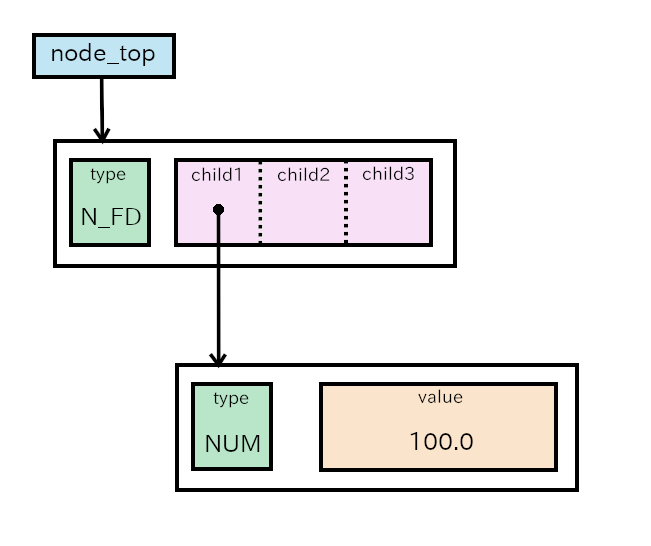
\includegraphics[width=6.51cm,height=5.46cm]{../image/tree.png}
\caption{tree}
\end{figure}

The following is the grammar rule extracted from
\passthrough{\lstinline!turtle.y!}. The rules there are based on the
same idea above. I don't want to explain the whole rules below. Please
look into each line carefully so that you will understand all the rules
and actions.

\begin{lstlisting}
program:
  statement { node_top = $$ = $1; }
| program statement {
        node_top = $$ = tree1 (N_program, $1, $2, NULL);
        }
;

statement:
  primary_procedure
| procedure_definition
;

primary_procedure:
  PU    { $$ = tree1 (N_PU, NULL, NULL, NULL); }
| PD    { $$ = tree1 (N_PD, NULL, NULL, NULL); }
| PW expression    { $$ = tree1 (N_PW, $2, NULL, NULL); }
| FD expression    { $$ = tree1 (N_FD, $2, NULL, NULL); }
| TR expression    { $$ = tree1 (N_TR, $2, NULL, NULL); }
| BC '(' expression ',' expression ',' expression ')' { $$ = tree1 (N_BC, $3, $5, $7); }
| FC '(' expression ',' expression ',' expression ')' { $$ = tree1 (N_FC, $3, $5, $7); }
 /* assignment */
| ID '=' expression   { $$ = tree1 (N_ASSIGN, tree3 (N_ID, $1), $3, NULL); }
 /* control flow */
| IF '(' expression ')' '{' primary_procedure_list '}' { $$ = tree1 (N_IF, $3, $6, NULL); }
| RT    { $$ = tree1 (N_RT, NULL, NULL, NULL); }
| RS    { $$ = tree1 (N_RS, NULL, NULL, NULL); }
 /* user defined procedure call */
| ID '(' ')'  { $$ = tree1 (N_procedure_call, tree3 (N_ID, $1), NULL, NULL); }
| ID '(' argument_list ')'  { $$ = tree1 (N_procedure_call, tree3 (N_ID, $1), $3, NULL); }
;

procedure_definition:
  DP ID '('  ')' '{' primary_procedure_list '}'  {
         $$ = tree1 (N_procedure_definition, tree3 (N_ID, $2), NULL, $6);
        }
| DP ID '(' parameter_list ')' '{' primary_procedure_list '}'  {
         $$ = tree1 (N_procedure_definition, tree3 (N_ID, $2), $4, $7);
        }
;

parameter_list:
  ID { $$ = tree3 (N_ID, $1); }
| parameter_list ',' ID  { $$ = tree1 (N_parameter_list, $1, tree3 (N_ID, $3), NULL); }
;

argument_list:
  expression
| argument_list ',' expression { $$ = tree1 (N_argument_list, $1, $3, NULL); }
;

primary_procedure_list:
  primary_procedure
| primary_procedure_list primary_procedure {
         $$ = tree1 (N_primary_procedure_list, $1, $2, NULL);
        }
;

expression:
  expression '=' expression { $$ = tree1 (N_EQ, $1, $3, NULL); }
| expression '>' expression { $$ = tree1 (N_GT, $1, $3, NULL); }
| expression '<' expression { $$ = tree1 (N_LT, $1, $3, NULL); }
| expression '+' expression { $$ = tree1 (N_ADD, $1, $3, NULL); }
| expression '-' expression { $$ = tree1 (N_SUB, $1, $3, NULL); }
| expression '*' expression { $$ = tree1 (N_MUL, $1, $3, NULL); }
| expression '/' expression { $$ = tree1 (N_DIV, $1, $3, NULL); }
| '-' expression %prec UMINUS { $$ = tree1 (N_UMINUS, $2, NULL, NULL); }
| '(' expression ')' { $$ = $2; }
| ID    { $$ = tree3 (N_ID, $1); }
| NUM   { $$ = tree2 (N_NUM, $1); }
;
\end{lstlisting}

\hypertarget{epilogue}{%
\subsubsection{Epilogue}\label{epilogue}}

The epilogue is written in C language and copied to the parser
implementation file. Generally, you can put anything into the epilogue.
In the case of turtle interpreter, the runtime routine and some other
functions are in the epilogue.

\hypertarget{functions-to-create-tree-nodes}{%
\paragraph{Functions to create tree
nodes}\label{functions-to-create-tree-nodes}}

There are three functions, \passthrough{\lstinline!tree1!},
\passthrough{\lstinline!tree2!} and \passthrough{\lstinline!tree3!}.

\begin{itemize}
\tightlist
\item
  \passthrough{\lstinline!tree1!} creates a node and sets the node type
  and pointers to its three children (NULL is possible).
\item
  \passthrough{\lstinline!tree2!} creates a node and sets the node type
  and a value (double).
\item
  \passthrough{\lstinline!tree3!} creates a node and sets the node type
  and a pointer to a string.
\end{itemize}

Each function gets memories first and build a node on them. The memories
are inserted to the list. They will be freed when runtime routine
finishes.

The three functions are called in the actions in the rules section.

\begin{lstlisting}[language=C]
/* Dynamically allocated memories are added to the single list. They will be freed in the finalize function. */
GSList *list = NULL;

node_t *
tree1 (int type, node_t *child1, node_t *child2, node_t *child3) {
  node_t *new_node;

  list = g_slist_prepend (list, g_malloc (sizeof (node_t)));
  new_node = (node_t *) list->data;
  new_node->type = type;
  child1(new_node) = child1;
  child2(new_node) = child2;
  child3(new_node) = child3;
  return new_node;
}

node_t *
tree2 (int type, double value) {
  node_t *new_node;

  list = g_slist_prepend (list, g_malloc (sizeof (node_t)));
  new_node = (node_t *) list->data;
  new_node->type = type;
  value(new_node) = value;
  return new_node;
}

node_t *
tree3 (int type, char *name) {
  node_t *new_node;

  list = g_slist_prepend (list, g_malloc (sizeof (node_t)));
  new_node = (node_t *) list->data;
  new_node->type = type;
  name(new_node) = name;
  return new_node;
}
\end{lstlisting}

\hypertarget{symbol-table}{%
\paragraph{Symbol table}\label{symbol-table}}

Variables and user defined procedures are registered in a symbol table.
This table is a C array. It should be replaced by more appropriate data
structure with memory allocation in the future version

\begin{itemize}
\tightlist
\item
  Variables are registered with its name and value.
\item
  Procedures are registered with its name and a pointer to the node of
  the procedure.
\end{itemize}

Therefore the table has the following fields.

\begin{itemize}
\tightlist
\item
  type to identify variable or procedure
\item
  name
\item
  value or pointer to a node
\end{itemize}

\begin{lstlisting}[language=C]
#define MAX_TABLE_SIZE 100
enum {
  PROC,
  VAR
};

typedef union _object_t object_t;
union _object_t {
  node_t *node;
  double value;
};

struct {
  int type;
  char *name;
  object_t object;
} table[MAX_TABLE_SIZE];
int tp;

void
init_table (void) {
  tp = 0;
}
\end{lstlisting}

\passthrough{\lstinline!init\_table!} initializes the table. This must
be called before any registrations.

There are five functions to access the table,

\begin{itemize}
\tightlist
\item
  \passthrough{\lstinline!proc\_install!} installs a procedure.
\item
  \passthrough{\lstinline!var\_install!} installs a variable.
\item
  \passthrough{\lstinline!proc\_lookup!} looks up a procedure. If the
  procedure is found, it returns a pointer to the node. Otherwise it
  returns NULL.
\item
  \passthrough{\lstinline!var\_lookup!} looks up a variable. If the
  variable is found, it returns TRUE and sets the pointer (argument) to
  point the value. Otherwise it returns FALSE.
\item
  \passthrough{\lstinline!var\_replace!} replaces the value of a
  variable. If the variable hasn't registered yet, it installs the
  variable.
\end{itemize}

\begin{lstlisting}[language=C]
int
tbl_lookup (int type, char *name) {
  int i;

  if (tp == 0)
    return -1;
  for (i=0; i<tp; ++i)
    if (type == table[i].type && strcmp(name, table[i].name) == 0)
      return i;
  return -1;
}

void
tbl_install (int type, char *name, object_t object) {
  if (tp >= MAX_TABLE_SIZE)
    runtime_error ("Symbol table overflow.\n");
  else if (tbl_lookup (type, name) >= 0)
    runtime_error ("Name %s is already registered.\n", name);
  else {
    table[tp].type = type;
    table[tp].name = name;
    if (type == PROC)
      table[tp++].object.node = object.node;
    else
      table[tp++].object.value = object.value;
  }
}

void
proc_install (char *name, node_t *node) {
  object_t object;
  object.node = node;
  tbl_install (PROC, name, object);
}

void
var_install (char *name, double value) {
  object_t object;
  object.value = value;
  tbl_install (VAR, name, object);
}

void
var_replace (char *name, double value) {
  int i;
  if ((i = tbl_lookup (VAR, name)) >= 0)
    table[i].object.value = value;
  else
    var_install (name, value);
}

node_t *
proc_lookup (char *name) {
  int i;
  if ((i = tbl_lookup (PROC, name)) < 0)
    return NULL;
  else
    return table[i].object.node;
}

gboolean
var_lookup (char *name, double *value) {
  int i;
  if ((i = tbl_lookup (VAR, name)) < 0)
    return FALSE;
  else {
    *value = table[i].object.value;
    return TRUE;
  }
}
\end{lstlisting}

\hypertarget{stack-for-parameters-and-arguments}{%
\paragraph{Stack for parameters and
arguments}\label{stack-for-parameters-and-arguments}}

Stack is a last-in first-out data structure. It is shortened to LIFO.
Turtle uses a stack to keep parameters and arguments. They are like
\passthrough{\lstinline!auto!} class variables in C language. They are
pushed to the stack whenever the procedure is called. LIFO structure is
useful for recursive calls.

Each element of the stack has name and value.

\begin{lstlisting}[language=C]
#define MAX_STACK_SIZE 500
struct {
  char *name;
  double value;
} stack[MAX_STACK_SIZE];
int sp, sp_biggest;

void
init_stack (void) {
  sp = sp_biggest = 0;
}
\end{lstlisting}

\passthrough{\lstinline!sp!} is a stack pointer. It is an index of the
array \passthrough{\lstinline!stack!} and it always points an element of
the array to store the next data. \passthrough{\lstinline!sp\_biggest!}
is the biggest number assigned to \passthrough{\lstinline!sp!}. We can
know the amount of elements used in the array during the runtime. The
purpose of the variable is to find appropriate
\passthrough{\lstinline!MAX\_STACK\_SIZE!}. It will be unnecessary in
the future version if the stack is implemented with better data
structure and memory allocation.

The runtime routine push data to the stack when it executes a node of a
procedure call. (The type of the node is
\passthrough{\lstinline!N\_procedure\_call!}.)

\begin{lstlisting}
dp drawline (angle, distance) { ... ... ... }
drawline (90, 100)
\end{lstlisting}

\begin{itemize}
\tightlist
\item
  The first line defines a procedure \passthrough{\lstinline!drawline!}.
  The runtime routine stores the name \passthrough{\lstinline!drawline!}
  and the node of the procedure to the symbol table.
\item
  The second line calls the procedure. First, it looks for the procedure
  in the symbol table and gets its node. Then it searches the node for
  the parameters and gets \passthrough{\lstinline!angle!} and
  \passthrough{\lstinline!distance!}.
\item
  It pushes (``distance'', 100.0) to the stack.
\item
  It pushes (``angle'', 90.0) to the stack.
\item
  It pushes (NULL, 2.0) to the stack. The number 2.0 is the number of
  parameters (or arguments). It is used when the procedure returns.
\end{itemize}

The following diagram shows the structure of the stack. First,
\passthrough{\lstinline!procedure 1!} is called. The procedure has two
parameters. In the \passthrough{\lstinline!procedure 1!}, another
procedure \passthrough{\lstinline!procedure 2!}, which has one
parameter, is called. And in the \passthrough{\lstinline!procedure 2!},
\passthrough{\lstinline!procedure 3!}, which has three parameters, is
called.

Programs push data to a stack from a low address memory to a high
address memory. In the following diagram, the lowest address is at the
top and the highest address is at the bottom. That is the order of the
address. However, ``the top of the stack'' is the last pushed data and
``the bottom of the stack'' is the first pushed data. Therefore, ``the
top of the stack'' is the bottom of the rectangle in the diagram and
``the bottom of the stack'' is the top of the rectangle.

\begin{figure}
\centering
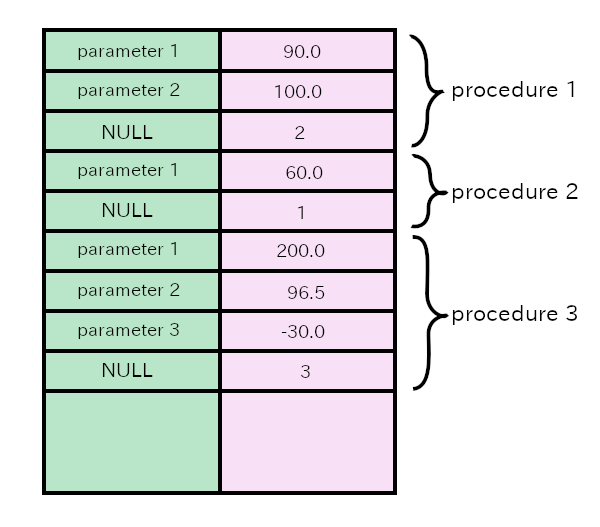
\includegraphics[width=6.64cm,height=8.05cm]{../image/stack.png}
\caption{Stack}
\end{figure}

There are four functions to access the stack.

\begin{itemize}
\tightlist
\item
  \passthrough{\lstinline!stack\_push!} pushes data to the stack.
\item
  \passthrough{\lstinline!stack\_lookup!} searches the stack for the
  variable given its name as an argument. It searches only the
  parameters of the latest procedure. It returns TRUE and sets the
  argument \passthrough{\lstinline!value!} to point the value, if the
  variable has been found. Otherwise it returns FALSE.
\item
  \passthrough{\lstinline!stack\_replace!} replaces the value of the
  variable in the stack. If it succeeds, it returns TRUE. Otherwise
  returns FALSE.
\item
  \passthrough{\lstinline!stack\_return!} throws away the latest
  parameters. The stack pointer goes back to the point before the latest
  procedure call so that it points to parameters of the previous called
  procedure.
\end{itemize}

\begin{lstlisting}[language=C]
void
stack_push (char *name, double value) {
  if (sp >= MAX_STACK_SIZE)
    runtime_error ("Stack overflow.\n");
  else {
    stack[sp].name = name;
    stack[sp++].value = value;
    sp_biggest = sp > sp_biggest ? sp : sp_biggest;
  }
}

int
stack_search (char *name) {
  int depth, i;

  if (sp == 0)
    return -1;
  depth = (int) stack[sp-1].value;
  if (depth + 1 > sp) /* something strange */
    runtime_error ("Stack error.\n");
  for (i=0; i<depth; ++i)
    if (strcmp(name, stack[sp-(i+2)].name) == 0) {
      return sp-(i+2);
    }
  return -1;
}

gboolean
stack_lookup (char *name, double *value) {
  int i;

  if ((i = stack_search (name)) < 0)
    return FALSE;
  else {
    *value = stack[i].value;
    return TRUE;
  }
}

gboolean
stack_replace (char *name, double value) {
  int i;

  if ((i = stack_search (name)) < 0)
    return FALSE;
  else {
    stack[i].value = value;
    return TRUE;
  }
}

void
stack_return(void) {
  int depth;

  if (sp <= 0)
    return;
  depth = (int) stack[sp-1].value;
  if (depth + 1 > sp) /* something strange */
    runtime_error ("Stack error.\n");
  sp -= depth + 1;
}
\end{lstlisting}

\hypertarget{surface-and-cairo}{%
\paragraph{Surface and cairo}\label{surface-and-cairo}}

A global variable \passthrough{\lstinline!surface!} is shared by
\passthrough{\lstinline!turtleapplication.c!} and
\passthrough{\lstinline!turtle.y!}. It is initialized in
\passthrough{\lstinline!turtleapplication.c!}.

The runtime routine has its own cairo context. This is different from
the cairo of GtkDrawingArea. Runtime routine draws a shape on the
\passthrough{\lstinline!surface!} with the cairo context. After runtime
routine returns to \passthrough{\lstinline!run\_cb!},
\passthrough{\lstinline!run\_cb!} adds the GtkDrawingArea widget to the
queue to redraw. When the widget is redraw,the drawing function
\passthrough{\lstinline!draw\_func!} is called. It copies the
\passthrough{\lstinline!surface!} to the surface in the GtkDrawingArea
object.

\passthrough{\lstinline!turtle.y!} has two functions
\passthrough{\lstinline!init\_cairo!} and
\passthrough{\lstinline!destroy\_cairo!}.

\begin{itemize}
\tightlist
\item
  \passthrough{\lstinline!init\_cairo!} initializes static variables and
  cairo context. The variables keep pen status (up or down), direction,
  initial location, line width and color. The size of the
  \passthrough{\lstinline!surface!} changes according to the size of the
  window. Whenever a user drags and resizes the window, the
  \passthrough{\lstinline!surface!} is also resized.
  \passthrough{\lstinline!init\_cairo!} gets the size first and sets the
  initial location of the turtle (center of the surface) and the
  transformation matrix.
\item
  \passthrough{\lstinline!destroy\_cairo!} just destroys the cairo
  context.
\end{itemize}

Turtle has its own coordinate. The origin is at the center of the
surface, and positive direction of x and y axes are right and up
respectively. But surfaces have its own coordinate. Its origin is at the
top-left corner of the surface and positive direction of x and y are
right and down respectively. A plane with the turtle's coordinate is
called user space, which is the same as cairo's user space. A plane with
the surface's coordinate is called device space.

Cairo provides a transformation which is an affine transformation. It
transforms a user-space coordinate (x, y) into a device-space coordinate
(z, w).

\begin{figure}
\centering
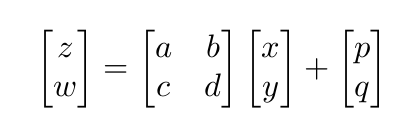
\includegraphics[width=6.3cm,height=2.04cm]{../image/transformation.png}
\caption{transformation}
\end{figure}

\passthrough{\lstinline!init\_cairo!} gets the width and height of the
\passthrough{\lstinline!surface!} (See the program below).

\begin{itemize}
\tightlist
\item
  The center of the surface is (0,0) with regard to the user-space
  coordinate and (width/2, height/2) with regard to the device-space
  coordinate.
\item
  The positive direction of x axis in the two spaces are the same. So,
  (1,0) is transformed into (1+width/2,height/2).
\item
  The positive direction of y axis in the two spaces are opposite. So,
  (0,1) is transformed into (width/2,-1+height/2).
\end{itemize}

You can determine a, b, c, d, p and q by substituting the numbers above
for x, y, z and w in the equation above. The solution of the
simultaneous equations is:

\begin{lstlisting}
a = 1, b = 0, c = 0, d = -1, p = width/2, q = height/2
\end{lstlisting}

Cairo provides a structure \passthrough{\lstinline!cairo\_matrix\_t!}.
\passthrough{\lstinline!init\_cairo!} uses it and sets the cairo
transformation (See the program below). Once the matrix is set, the
transformation always performs whenever
\passthrough{\lstinline!cairo\_stroke!} function is invoked.

\begin{lstlisting}[language=C]
/* status of the surface */
static gboolean pen = TRUE;
static double angle = 90.0; /* angle starts from x axis and measured counterclockwise */
                   /* Initially facing to the north */
static double cur_x = 0.0;
static double cur_y = 0.0;
static double line_width = 2.0;

struct color {
  double red;
  double green;
  double blue;
};
static struct color bc = {0.95, 0.95, 0.95}; /* white */
static struct color fc = {0.0, 0.0, 0.0}; /* black */

/* cairo */
static cairo_t *cr;
gboolean
init_cairo (void) {
  int width, height;
  cairo_matrix_t matrix;

  pen = TRUE;
  angle = 90.0;
  cur_x = 0.0;
  cur_y = 0.0;
  line_width = 2.0;
  bc.red = 0.95; bc.green = 0.95; bc.blue = 0.95;
  fc.red = 0.0; fc.green = 0.0; fc.blue = 0.0;

  if (surface) {
    width = cairo_image_surface_get_width (surface);
    height = cairo_image_surface_get_height (surface);
    matrix.xx = 1.0; matrix.xy = 0.0; matrix.x0 = (double) width / 2.0;
    matrix.yx = 0.0; matrix.yy = -1.0; matrix.y0 = (double) height / 2.0;

    cr = cairo_create (surface);
    cairo_transform (cr, &matrix);
    cairo_set_source_rgb (cr, bc.red, bc.green, bc.blue);
    cairo_paint (cr);
    cairo_set_source_rgb (cr, fc.red, fc.green, fc.blue);
    cairo_move_to (cr, cur_x, cur_y);
    return TRUE;
  } else
    return FALSE;
}

void
destroy_cairo () {
  cairo_destroy (cr);
}
\end{lstlisting}

\hypertarget{eval-function}{%
\paragraph{Eval function}\label{eval-function}}

A function \passthrough{\lstinline!eval!} evaluates an expression and
returns the value of the expression. It calls itself recursively. For
example, if the node is \passthrough{\lstinline!N\_ADD!}, then:

\begin{enumerate}
\def\labelenumi{\arabic{enumi}.}
\tightlist
\item
  Calls eval(child1(node)) and gets the value1.
\item
  Calls eval(child2(node)) and gets the value2.
\item
  Returns value1+value2.
\end{enumerate}

This is performed by a macro \passthrough{\lstinline!calc!} defined in
the sixth line in the following program.

\begin{lstlisting}[language=C]
double
eval (node_t *node) {
double value = 0.0;
  if (node == NULL)
    runtime_error ("No expression to evaluate.\n");
#define calc(op) eval (child1(node)) op eval (child2(node))
  switch (node->type) {
    case N_EQ:
      value = (double) calc(==);
      break;
    case N_GT:
      value = (double) calc(>);
      break;
    case N_LT:
      value = (double) calc(<);
      break;
    case N_ADD:
      value = calc(+);
      break;
    case N_SUB:
      value = calc(-);
      break;
    case N_MUL:
      value = calc(*);
      break;
    case N_DIV:
      if (eval (child2(node)) == 0.0)
        runtime_error ("Division by zerp.\n");
      else
        value = calc(/);
      break;
    case N_UMINUS:
      value = -(eval (child1(node)));
      break;
    case N_ID:
      if (! (stack_lookup (name(node), &value)) && ! var_lookup (name(node), &value) )
        runtime_error ("Variable %s not defined.\n", name(node));
      break;
    case N_NUM:
      value = value(node);
      break;
    default:
      runtime_error ("Illegal expression.\n");
  }
  return value;
}
\end{lstlisting}

\hypertarget{execute-function}{%
\paragraph{Execute function}\label{execute-function}}

Primary procedures and procedure definitions are analyzed and executed
by the function \passthrough{\lstinline!execute!}. It doesn't return any
values. It calls itself recursively. The process of
\passthrough{\lstinline!N\_RT!} and
\passthrough{\lstinline!N\_procedure\_call!} is complicated. It will
explained after the following program. Other parts are not so difficult.
Read the program below carefully so that you will understand the
process.

\begin{lstlisting}[language=C]
/* procedure - return status */
static int proc_level = 0;
static int ret_level = 0;

void
execute (node_t *node) {
  double d, x, y;
  char *name;
  int n, i;

  if (node == NULL)
    runtime_error ("Node is NULL.\n");
  if (proc_level > ret_level)
    return;
  switch (node->type) {
    case N_program:
      execute (child1(node));
      execute (child2(node));
      break;
    case N_PU:
      pen = FALSE;
      break;
    case N_PD:
      pen = TRUE;
      break;
    case N_PW:
      line_width = eval (child1(node)); /* line width */
      break;
    case N_FD:
      d = eval (child1(node)); /* distance */
      x = d * cos (angle*M_PI/180);
      y = d * sin (angle*M_PI/180);
      /* initialize the current point = start point of the line */
      cairo_move_to (cr, cur_x, cur_y);
      cur_x += x;
      cur_y += y;
      cairo_set_line_width (cr, line_width);
      cairo_set_source_rgb (cr, fc.red, fc.green, fc.blue);
      if (pen)
        cairo_line_to (cr, cur_x, cur_y);
      else
        cairo_move_to (cr, cur_x, cur_y);
      cairo_stroke (cr);
      break;
    case N_TR:
      angle -= eval (child1(node));
      for (; angle < 0; angle += 360.0);
      for (; angle>360; angle -= 360.0);
      break;
    case N_BC:
      bc.red = eval (child1(node));
      bc.green = eval (child2(node));
      bc.blue = eval (child3(node));
#define fixcolor(c)  c = c < 0 ? 0 : (c > 1 ? 1 : c)
      fixcolor (bc.red);
      fixcolor (bc.green);
      fixcolor (bc.blue);
      /* clear the shapes and set the background color */
      cairo_set_source_rgb (cr, bc.red, bc.green, bc.blue);
      cairo_paint (cr);
      break;
    case N_FC:
      fc.red = eval (child1(node));
      fc.green = eval (child2(node));
      fc.blue = eval (child3(node));
      fixcolor (fc.red);
      fixcolor (fc.green);
      fixcolor (fc.blue);
      break;
    case N_ASSIGN:
      name = name(child1(node));
      d = eval (child2(node));
      if (! stack_replace (name, d)) /* First, tries to replace the value in the stack (parameter).*/
        var_replace (name, d); /* If the above fails, tries to replace the value in the table. If the variable isn't in the table, installs it, */
      break;
    case N_IF:
      if (eval (child1(node)))
        execute (child2(node));
      break;
    case N_RT:
      ret_level--;
      break;
    case N_RS:
      pen = TRUE;
      angle = 90.0;
      cur_x = 0.0;
      cur_y = 0.0;
      line_width = 2.0;
      fc.red = 0.0; fc.green = 0.0; fc.blue = 0.0;
      /* To change background color, use bc. */
      break;
    case N_procedure_call:
      name = name(child1(node));
node_t *proc = proc_lookup (name);
      if (! proc)
        runtime_error ("Procedure %s not defined.\n", name);
      if (strcmp (name, name(child1(proc))) != 0)
        runtime_error ("Unexpected error. Procedure %s is called, but invoked procedure is %s.\n", name, name(child1(proc)));
/* make tuples (parameter (name), argument (value)) and push them to the stack */
node_t *param_list;
node_t *arg_list;
      param_list = child2(proc);
      arg_list = child2(node);
      if (param_list == NULL) {
        if (arg_list == NULL) {
          stack_push (NULL, 0.0); /* number of argument == 0 */
        } else
          runtime_error ("Procedure %s has different number of argument and parameter.\n", name);
      }else {
/* Don't change the stack until finish evaluating the arguments. */
#define TEMP_STACK_SIZE 20
        char *temp_param[TEMP_STACK_SIZE];
        double temp_arg[TEMP_STACK_SIZE];
        n = 0;
        for (; param_list->type == N_parameter_list; param_list = child1(param_list)) {
          if (arg_list->type != N_argument_list)
            runtime_error ("Procedure %s has different number of argument and parameter.\n", name);
          if (n >= TEMP_STACK_SIZE)
            runtime_error ("Too many parameters. the number must be %d or less.\n", TEMP_STACK_SIZE);
          temp_param[n] = name(child2(param_list));
          temp_arg[n] = eval (child2(arg_list));
          arg_list = child1(arg_list);
          ++n;
        }
        if (param_list->type == N_ID && arg_list -> type != N_argument_list) {
          temp_param[n] = name(param_list);
          temp_arg[n] = eval (arg_list);
          if (++n >= TEMP_STACK_SIZE)
            runtime_error ("Too many parameters. the number must be %d or less.\n", TEMP_STACK_SIZE);
          temp_param[n] = NULL;
          temp_arg[n] = (double) n;
          ++n;
        } else
          runtime_error ("Unexpected error.\n");
        for (i = 0; i < n; ++i)
          stack_push (temp_param[i], temp_arg[i]);
      }
      ret_level = ++proc_level;
      execute (child3(proc));
      ret_level = --proc_level;
      stack_return ();
      break;
    case N_procedure_definition:
      name = name(child1(node));
      proc_install (name, node);
      break;
    case N_primary_procedure_list:
      execute (child1(node));
      execute (child2(node));
      break;
    default:
      runtime_error ("Unknown statement.\n");
  }
}
\end{lstlisting}

A node \passthrough{\lstinline!N\_procedure\_call!} is created by the
parser when it has found a user defined procedure call. The procedure
has been defined in the prior statement. Suppose the parser reads the
following example code.

\begin{lstlisting}
dp drawline (angle, distance) {
  tr angle
  fd distance
}
drawline (90, 100)
drawline (90, 100)
drawline (90, 100)
drawline (90, 100)
\end{lstlisting}

This example draws a square.

When The parser reads the lines from one to four, it creates nodes like
this:

\begin{figure}
\centering
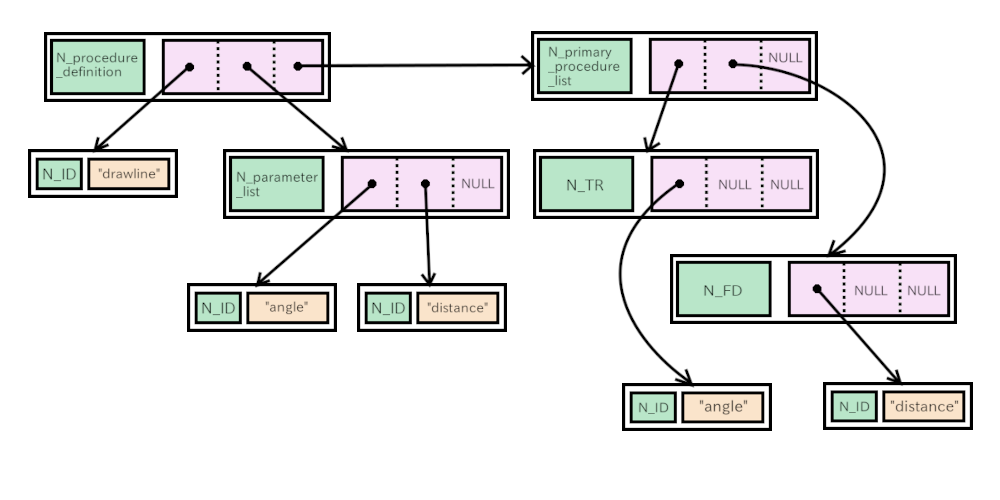
\includegraphics[width=10cm,height=6cm]{../image/tree2.png}
\caption{Nodes of drawline}
\end{figure}

Runtime routine just stores the procedure to the symbol table with its
name and node.

\begin{figure}
\centering
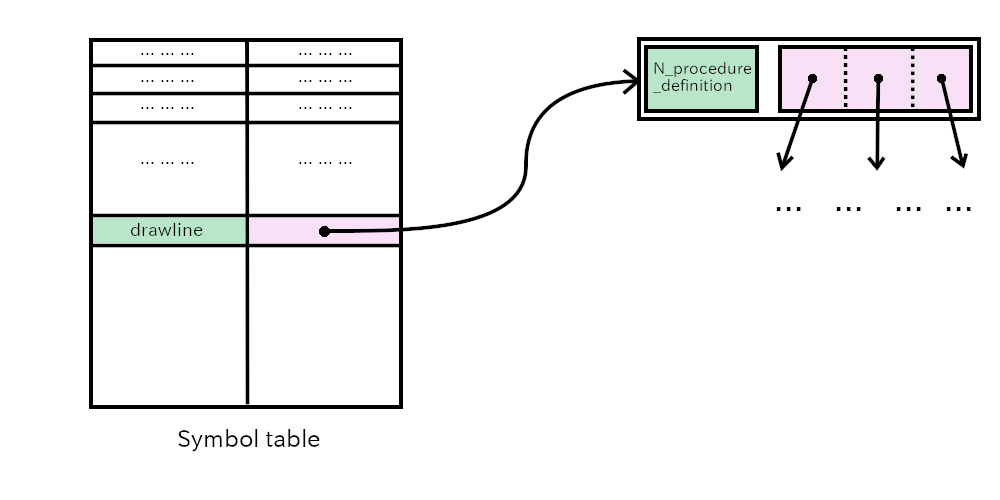
\includegraphics[width=10cm,height=5cm]{../image/table.png}
\caption{Symbol table}
\end{figure}

When the parser reads the fifth line in the example, it creates nodes
like this:

\begin{figure}
\centering
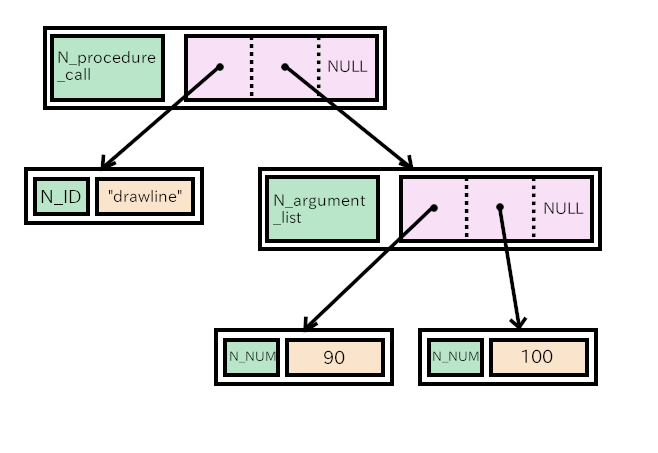
\includegraphics[width=10cm,height=5cm]{../image/proc_call.png}
\caption{Nodes of procedure call}
\end{figure}

When the runtime routine meets
\passthrough{\lstinline!N\_procedure\_call!} node, it behaves like this:

\begin{enumerate}
\def\labelenumi{\arabic{enumi}.}
\tightlist
\item
  Searches the symbol table for the procedure with the name.
\item
  Gets pointers to the node to parameters and the node to the body.
\item
  Creates a temporary stack. Makes a tuple of each parameter name and
  argument value. Pushes the tuples into the stack, and (NULL, number of
  parameters) finally. If no error occurs, copies them from the
  temporary stack to the parameter stack.
\item
  Increases \passthrough{\lstinline!prc\_level!} by one. Sets
  \passthrough{\lstinline!ret\_level!} to the same value as
  \passthrough{\lstinline!proc\_level!}.
  \passthrough{\lstinline!proc\_level!} is zero when runtime routine
  runs on the main routine. If it goes into a procedure,
  \passthrough{\lstinline!proc\_level!} increases by one. Therefore,
  \passthrough{\lstinline!proc\_level!} is the depth of the procedure
  call. \passthrough{\lstinline!ret\_level!} is the level to return. If
  it is the same as \passthrough{\lstinline!proc\_level!}, runtime
  routine executes commands in order of the commands in the procedure.
  If it is smaller than \passthrough{\lstinline!proc\_level!}, runtime
  routine doesn't execute commands until it becomes the same level as
  \passthrough{\lstinline!proc\_level!}.
  \passthrough{\lstinline!ret\_level!} is used to return the procedure.
\item
  Executes the node of the body of the procedure.
\item
  Decreases \passthrough{\lstinline!proc\_level!} by one. Sets
  \passthrough{\lstinline!ret\_level!} to the same value as
  \passthrough{\lstinline!proc\_level!}. Calls
  \passthrough{\lstinline!stack\_return!}.
\end{enumerate}

When the runtime routine meets \passthrough{\lstinline!N\_RT!} node, it
decreases \passthrough{\lstinline!ret\_level!} by one so that the
following commands in the procedure are ignored by the runtime routine.

\hypertarget{runtime-entry-and-error-functions}{%
\paragraph{Runtime entry and error
functions}\label{runtime-entry-and-error-functions}}

A function \passthrough{\lstinline!run!} is the entry of the runtime
routine. A function \passthrough{\lstinline!runtime\_error!} reports an
error occurred during the runtime routine runs. (Errors which occur
during the parsing are called syntax error and reported by
\passthrough{\lstinline!yyerror!}.) After
\passthrough{\lstinline!runtime\_error!} reports an error, it stops the
command execution and goes back to \passthrough{\lstinline!run!} to
exit.

Setjmp and longjmp functions are used. They are declared in
\passthrough{\lstinline!<setjmp.h>!}.
\passthrough{\lstinline!setjmp (buf)!} saves state information in
\passthrough{\lstinline!buf!} and returns zero.
\passthrough{\lstinline!longjmp(buf, 1)!} restores the state information
from \passthrough{\lstinline!buf!} and returns
\passthrough{\lstinline!1!} (the second argument). Because the
information is the status at the time \passthrough{\lstinline!setjmp!}
is called, so longjmp resumes the execution at the next of setjmp
function call. In the following program, longjmp resumes at the
assignment to the variable \passthrough{\lstinline!i!}. When setjmp is
called, 0 is assigned to \passthrough{\lstinline!i!} and
\passthrough{\lstinline!execute(node\_top)!} is called. On the other
hand, when longjmp is called, 1 is assigned to
\passthrough{\lstinline!i!} and
\passthrough{\lstinline!execute(node\_top)!} is not called..

\passthrough{\lstinline!g\_slist\_free\_full!} frees all the allocated
memories.

\begin{lstlisting}[language=C]
static jmp_buf buf;

void
run (void) {
  int i;

  if (! init_cairo()) {
    g_print ("Cairo not initialized.\n");
    return;
  }
  init_table();
  init_stack();
  ret_level = proc_level = 1;
  i = setjmp (buf);
  if (i == 0)
    execute(node_top);
  /* else ... get here by calling longjmp */
  destroy_cairo ();
  g_slist_free_full (g_steal_pointer (&list), g_free);
}

/* format supports only %s, %f and %d */
static void
runtime_error (char *format, ...) {
  va_list args;
  char *f;
  char b[3];
  char *s;
  double v;
  int i;

  va_start (args, format);
  for (f = format; *f; f++) {
    if (*f != '%') {
      b[0] = *f;
      b[1] = '\0';
      g_print ("%s", b);
      continue;
    }
    switch (*++f) {
      case 's':
        s = va_arg(args, char *);
        g_print ("%s", s);
        break;
      case 'f':
        v = va_arg(args, double);
        g_print("%f", v);
        break;
      case 'd':
        i = va_arg(args, int);
        g_print("%d", i);
        break;
      default:
        b[0] = '%';
        b[1] = *f;
        b[2] = '\0';
        g_print ("%s", b);
        break;
    }
  }
  va_end (args);

  longjmp (buf, 1);
}
\end{lstlisting}

A function \passthrough{\lstinline!runtime\_error!} has a
variable-length argument list.

\begin{lstlisting}[language=C]
void runtime_error (char *format, ...)
\end{lstlisting}

This is implemented with \passthrough{\lstinline!<stdarg.h>!} header
file. The \passthrough{\lstinline!va\_list!} type variable
\passthrough{\lstinline!args!} will refer to each argument in turn. A
function \passthrough{\lstinline!va\_start!} initializes
\passthrough{\lstinline!args!}. A function
\passthrough{\lstinline!va\_arg!} returns an argument and moves the
reference of \passthrough{\lstinline!args!} to the next. A function
\passthrough{\lstinline!va\_end!} cleans up everything necessary at the
end.

The function \passthrough{\lstinline!runtime\_error!} has a similar
format of printf standard function. But its format has only
\passthrough{\lstinline!\%s!}, \passthrough{\lstinline!\%f!} and
\passthrough{\lstinline!\%d!}.

The functions declared in \passthrough{\lstinline!<setjmp.h>!} and
\passthrough{\lstinline!<stdarg.h>!} are explained in the very famous
book ``The C programming language'' written by Brian Kernighan and
Dennis Ritchie. I referred to the book to write the program above.

The program \passthrough{\lstinline!turtle!} is unsophisticated and
unpolished. If you want to make your own language, you need to know more
and more. I don't know any good textbook about compilers and
interpreters. If you know a good book, please let me know.

However, the following information is very useful (but old).

\begin{itemize}
\tightlist
\item
  Bison documentation
\item
  Flex documentation
\item
  Software tools written by Brian W. Kernighan \& P. J. Plauger (1976)
\item
  Unix programming environment written by Brian W. Kernighan and Rob
  Pike (1984)
\item
  Source code of a language, for example, ruby.
\end{itemize}

Lately, lots of source codes are in the internet. Maybe reading source
codes are the most useful for programmers.

  \hypertarget{gtklistview}{%
\section{GtkListView}\label{gtklistview}}

Gtk4 has added new list objects GtkListView, GtkGridView and
GtkColumnView. The new feature is described in
\href{https://docs.gtk.org/gtk4/section-list-widget.html}{Gtk API
Reference, List Widget Overview}.

Gtk4 has other means to implement lists. They are GtkListBox and
GtkTreeView which are took over from Gtk3. There's an article in
\href{https://blog.gtk.org/2020/06/07/scalable-lists-in-gtk-4/}{Gtk
Development blog} about list widgets by Matthias Clasen. He described
why GtkListView are developed to replace GtkListBox and GtkTreeView.

I want to explain GtkListView and its related objects in this tutorial.

\hypertarget{outline}{%
\subsection{Outline}\label{outline}}

A list is a sequential data structure. For example, an ordered string
sequence ``one'', ``two'', ``three'', ``four'' is a list. Each element
of the list is called item. A list is like an array, but in many cases
it is implemented with pointers which point to the next item of the
list. And it has a start point. So, each item can be referred by the
index of the item (first item, second item, \ldots, nth item, \ldots).
There are two cases. One is the index starts from one (one-based) and
the other is it starts from zero (zero-based).

Gio provides GListModel interface. It is a zero-based list of the same
type of GObject objects, or objects that implement the same interface.
An object implements GListModel is usually not a widget. So, the list is
not displayed on the screen directly. There's another object GtkListView
which is a widget to display the list. The items in the list need to be
connected to the items in GtkListView. GtkListItemFactory object maps
items in the list to GListView.

\begin{figure}
\centering
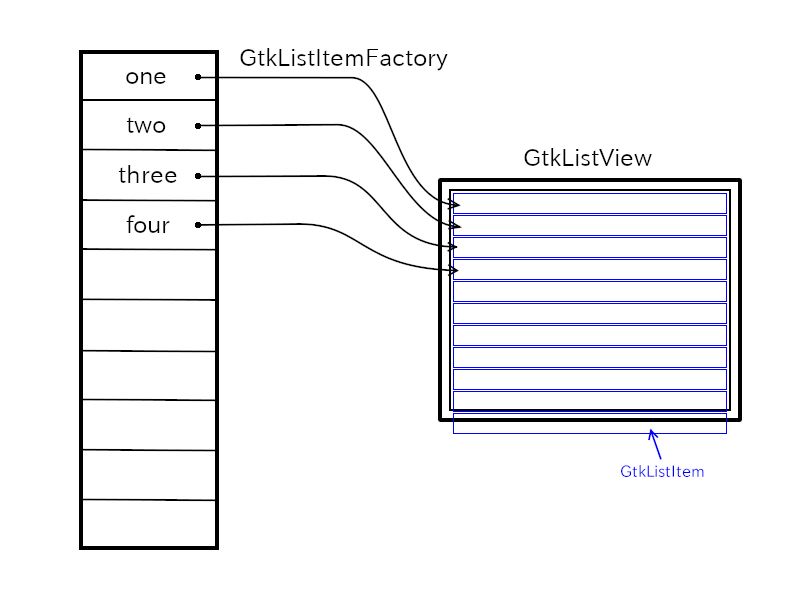
\includegraphics[width=10cm,height=7.5cm]{../image/list.png}
\caption{List}
\end{figure}

The instruction to build the whole list related objects is:

\begin{enumerate}
\def\labelenumi{\arabic{enumi}.}
\tightlist
\item
  Implement the list object which implements GListModel.
\item
  Build widgets and put GtkListView as a child of GtkScrolledWindow.
\item
  Set GtkListItemFactory.
\end{enumerate}

\hypertarget{glistmodel}{%
\subsection{GListModel}\label{glistmodel}}

If you want to make a list of strings with GListModel, for example,
``one'', ``two'', ``three'', ``four'', note that strings can't be items
of the list. Because GListModel is a list of GObject objects and strings
aren't GObject objects. So, you need a wrapper which is a GObject and
contains a string. GtkStringObject is the wrapper object and
GStringList, implements GListModel, is a list of GtkStringObject.

\begin{lstlisting}[language=C]
char *array[] = {"one", "two", "three", "four", NULL};
GtkStringList *stringlist = gtk_string_list_new ((const char * const *) array);
\end{lstlisting}

The function \passthrough{\lstinline!gtk\_string\_list\_new!} creates
GtkStringList object. Its items are GtkStringObject objects which
contain the strings ``one'', ``two'', ``three'' and ``four''. There are
functions to add items to the list or remove items from the list.

\begin{itemize}
\tightlist
\item
  \passthrough{\lstinline!gtk\_string\_list\_append!} appends an item to
  the list
\item
  \passthrough{\lstinline!gtk\_string\_list\_remove!} removes an item
  from the list
\item
  \passthrough{\lstinline!gtk\_string\_list\_get\_string!} gets a string
  in the list
\end{itemize}

See \href{https://docs.gtk.org/gtk4/class.StringList.html}{Gtk4 API
Reference, GtkStringList} for further information.

I'll explain the other list objects later.

\hypertarget{gtkselectionmodel}{%
\subsection{GtkSelectionModel}\label{gtkselectionmodel}}

GtkSelectionModel is an interface to support for selections. Thanks to
this model, user can select items by clicking on them. It is implemented
by GtkMultiSelection, GtkNoSelection and GtkSingleSelection objects.
These three objects are usually enough to build an application. They are
created with GListModel. You can also create them alone and add
GListModel later.

\begin{itemize}
\tightlist
\item
  GtkMultiSelection supports multiple selection.
\item
  GtkNoSelection supports no selection. This is a wrapper to GListModel
  when GtkSelectionModel is needed.
\item
  GtkSingleSelection supports single selection.
\end{itemize}

\hypertarget{gtklistview-1}{%
\subsection{GtkListView}\label{gtklistview-1}}

GtkListView is a widget to show GListModel items. GtkListItem is used by
GtkListView to represent items of a list model. But, GtkListItem itself
is not a widget, so a user needs to set a widget, for example GtkLabel,
as a child of GtkListItem to display an item of the list model. ``item''
property of GtkListItem points an object that belongs to the list model.

\begin{figure}
\centering
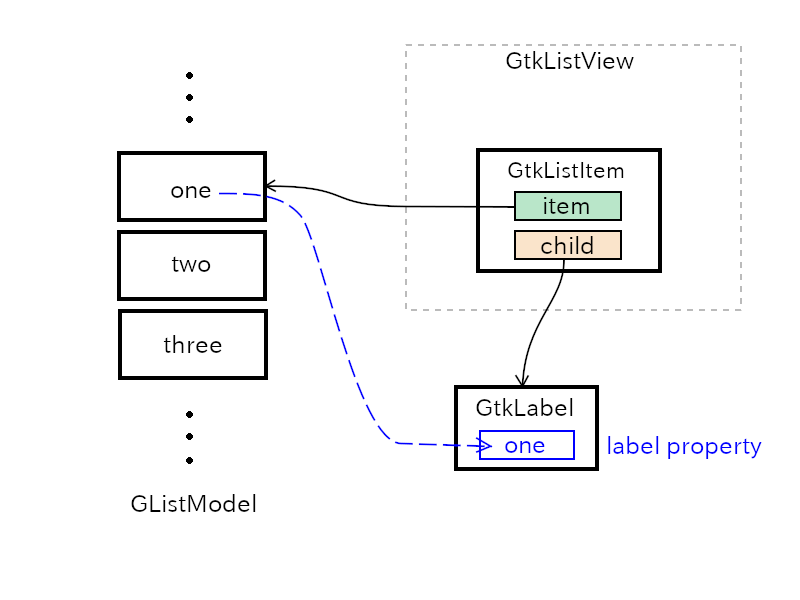
\includegraphics[width=10cm,height=7.5cm]{../image/gtklistitem.png}
\caption{GtkListItem}
\end{figure}

In case the number of items is very big, for example more than a
thousand, GtkListItem is recycled and connected to another item which is
newly displayed. This recycle makes the number of GtkListItem objects
fairly small, less than 200. This is very effective to restrain the
growth of memory consumption so that GListModel can contain lots of
items, for example, more than a million items.

\hypertarget{gtklistitemfactory}{%
\subsection{GtkListItemFactory}\label{gtklistitemfactory}}

GtkListItemFactory creates or recycles GtkListItem and connects it with
an item of the list model. There are two child objects of this factory,
GtkSignalListItemFactory and GtkBuilderListItemFactory.

\hypertarget{gtksignallistitemfactory}{%
\subsubsection{GtkSignalListItemFactory}\label{gtksignallistitemfactory}}

GtkSignalListItemFactory provides signals for users to configure a
GtkListItem object. There are four signals.

\begin{enumerate}
\def\labelenumi{\arabic{enumi}.}
\tightlist
\item
  ``setup'' is emitted to set up GtkListItem object. A user sets its
  child widget in the handler. For example, creates a GtkLabel widget
  and sets the child property of GtkListItem to it. This setting is kept
  even the GtkListItem instance is recycled (to bind to another item of
  GListModel).
\item
  ``bind'' is emitted to bind an item in the list model to the widget.
  For example, a user gets the item from ``item'' property of the
  GtkListItem instance. Then gets the string of the item and sets the
  label property of the GtkLabel instance with the string. This signal
  is emitted when the GtkListItem is newly created, recycled or some
  changes has happened to the item of the list.
\item
  ``unbind'' is emitted to unbind an item. A user undoes everything done
  in step 2 in the signal handler. If some object are created in step 2,
  they must be destroyed.
\item
  ``teardown'' is emitted to undo everything done in step 1. So, the
  widget created in step 1 must be destroyed. After this signal, the
  list item will be destroyed.
\end{enumerate}

The following program \passthrough{\lstinline!list1.c!} shows the list
of strings ``one'', ``two'', ``three'' and ``four''. GtkNoSelection is
used, so user can't select any item.

\begin{lstlisting}[language=C, numbers=left]
#include <gtk/gtk.h>

static void
setup_cb (GtkListItemFactory *factory, GtkListItem *listitem, gpointer user_data) {
  GtkWidget *lb = gtk_label_new (NULL);
  gtk_list_item_set_child (listitem, lb);
}

static void
bind_cb (GtkSignalListItemFactory *self, GtkListItem *listitem, gpointer user_data) {
  GtkWidget *lb = gtk_list_item_get_child (listitem);
  GtkStringObject *strobj = gtk_list_item_get_item (listitem);
  const char *text = gtk_string_object_get_string (strobj);

  gtk_label_set_text (GTK_LABEL (lb), text);
}

static void
unbind_cb (GtkSignalListItemFactory *self, GtkListItem *listitem, gpointer user_data) {
  /* There's nothing to do here. */
  /* If you does something like setting a signal in bind_cb, */
  /* then disconnecting the signal is necessary in unbind_cb. */
}

static void
teardown_cb (GtkListItemFactory *factory, GtkListItem *listitem, gpointer user_data) {
  gtk_list_item_set_child (listitem, NULL);
/*  When the child of listitem is set to NULL, the reference to GtkLabel will be released and lb will be destroyed. */
/* Therefore, g_object_unref () for the GtkLabel object doesn't need in the user code. */
}

/* ----- activate, open, startup handlers ----- */
static void
app_activate (GApplication *application) {
  GtkApplication *app = GTK_APPLICATION (application);
  GtkWidget *win = gtk_application_window_new (app);
  gtk_window_set_default_size (GTK_WINDOW (win), 600, 400);
  GtkWidget *scr = gtk_scrolled_window_new ();
  gtk_window_set_child (GTK_WINDOW (win), scr);

  char *array[] = {
    "one", "two", "three", "four", NULL
  };
  GtkStringList *sl = gtk_string_list_new ((const char * const *) array);
  GtkNoSelection *ns = gtk_no_selection_new (G_LIST_MODEL (sl));

  GtkListItemFactory *factory = gtk_signal_list_item_factory_new ();
  g_signal_connect (factory, "setup", G_CALLBACK (setup_cb), NULL);
  g_signal_connect (factory, "bind", G_CALLBACK (bind_cb), NULL);
  g_signal_connect (factory, "unbind", G_CALLBACK (unbind_cb), NULL);
  g_signal_connect (factory, "teardown", G_CALLBACK (teardown_cb), NULL);

  GtkWidget *lv = gtk_list_view_new (GTK_SELECTION_MODEL (ns), factory);
  gtk_scrolled_window_set_child (GTK_SCROLLED_WINDOW (scr), lv);
  gtk_widget_show (win);
}

static void
app_startup (GApplication *application) {
}

/* ----- main ----- */
#define APPLICATION_ID "com.github.ToshioCP.list1"

int
main (int argc, char **argv) {
  GtkApplication *app;
  int stat;

  app = gtk_application_new (APPLICATION_ID, G_APPLICATION_FLAGS_NONE);

  g_signal_connect (app, "startup", G_CALLBACK (app_startup), NULL);
  g_signal_connect (app, "activate", G_CALLBACK (app_activate), NULL);

  stat =g_application_run (G_APPLICATION (app), argc, argv);
  g_object_unref (app);
  return stat;
}
\end{lstlisting}

The file \passthrough{\lstinline!list1.c!} is located under the
directory src/misc. Make a shell script below and save it to your bin
directory. (If you've installed Gtk4 from the source to \$HOME/local,
then your bin directory is \$Home/local/bin. Otherwise, \$Home/bin is
your private bin directory.)

\begin{lstlisting}[language=bash]
gcc `pkg-config --cflags gtk4` $1.c `pkg-config --libs gtk4`
\end{lstlisting}

Change the current directory to the directory includes
\passthrough{\lstinline!list1.c!} and type as follows.

\begin{lstlisting}
$ chmod 755 $HOME/local/bin/comp # or chmod 755 $Home/bin/comp
$ comp list1
$ ./a.out
\end{lstlisting}

Then, \passthrough{\lstinline!list1.c!} has been compiled and executed.

\begin{figure}
\centering
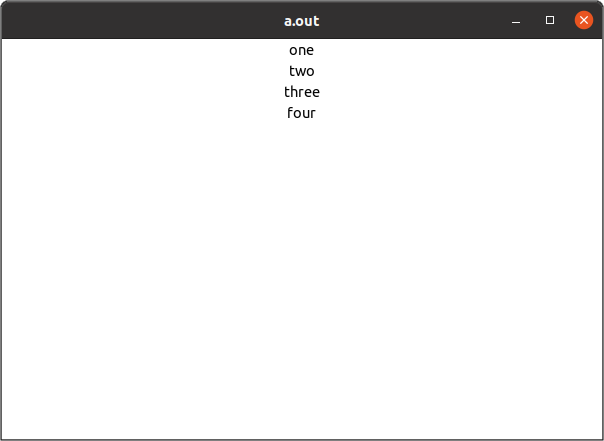
\includegraphics[width=6.04cm,height=4.4cm]{../image/list1.png}
\caption{list1}
\end{figure}

I think the program is not so difficult. If you feel some difficulty,
read this section again, especially GtkSignalListItemFactory
subsubsection.

\hypertarget{gtkbuilderlistitemfactory}{%
\subsubsection{GtkBuilderListItemFactory}\label{gtkbuilderlistitemfactory}}

GtkBuilderListItemFactory is another GtkListItemFactory. Its behavior is
defined with ui file.

\begin{lstlisting}[language=XML]
<interface>
  <template class="GtkListItem">
    <property name="child">
      <object class="GtkLabel">
        <binding name="label">
          <lookup name="string" type="GtkStringObject">
            <lookup name="item">GtkListItem</lookup>
          </lookup>
        </binding>
      </object>
    </property>
  </template>
</interface>
\end{lstlisting}

Template tag is used to define GtkListItem. And its child property is
GtkLabel object. The factory sees this template and creates GtkLabel and
sets the child property of GtkListItem. This is the same as what setup
handler of GtkSignalListItemFactory did.

Then, bind the label property of GtkLabel to string property of
GtkStringObject. The string object is referred to by item property of
GtkListItem. So, the lookup tag is like this:

\begin{lstlisting}
string <- GtkStringObject <- item <- GtkListItem
\end{lstlisting}

The last lookup tag has a content \passthrough{\lstinline!GtkListItem!}.
Usually, C type like \passthrough{\lstinline!GtkListItem!} doesn't
appear in the content of tags. This is a special case. There is an
explanation about it in the
\href{https://blog.gtk.org/2020/09/05/a-primer-on-gtklistview/}{GTK
Development Blog} by Matthias Clasen.

\begin{quote}
Remember that the classname (GtkListItem) in a ui template is used as
the ``this'' pointer referring to the object that is being instantiated.
\end{quote}

Therefore, GtkListItem instance is used as the
\passthrough{\lstinline!this!} object of the lookup tag when it is
evaluated. \passthrough{\lstinline!this!} object will be explained in
section 28.

The C source code is as follows. Its name is
\passthrough{\lstinline!list2.c!} and located under src/misc directory.

\begin{lstlisting}[language=C, numbers=left]
#include <gtk/gtk.h>

/* ----- activate, open, startup handlers ----- */
static void
app_activate (GApplication *application) {
  GtkApplication *app = GTK_APPLICATION (application);
  GtkWidget *win = gtk_application_window_new (app);
  gtk_window_set_default_size (GTK_WINDOW (win), 600, 400);
  GtkWidget *scr = gtk_scrolled_window_new ();
  gtk_window_set_child (GTK_WINDOW (win), scr);

  char *array[] = {
    "one", "two", "three", "four", NULL
  };
  GtkStringList *sl = gtk_string_list_new ((const char * const *) array);
  GtkSingleSelection *ss = gtk_single_selection_new (G_LIST_MODEL (sl));

  const char *ui_string =
"<interface>"
  "<template class=\"GtkListItem\">"
    "<property name=\"child\">"
      "<object class=\"GtkLabel\">"
        "<binding name=\"label\">"
          "<lookup name=\"string\" type=\"GtkStringObject\">"
            "<lookup name=\"item\">GtkListItem</lookup>"
          "</lookup>"
        "</binding>"
      "</object>"
    "</property>"
  "</template>"
"</interface>"
;
  GBytes *gbytes = g_bytes_new_static (ui_string, strlen (ui_string));
  GtkListItemFactory *factory = gtk_builder_list_item_factory_new_from_bytes (NULL, gbytes);

  GtkWidget *lv = gtk_list_view_new (GTK_SELECTION_MODEL (ss), factory);
  gtk_scrolled_window_set_child (GTK_SCROLLED_WINDOW (scr), lv);
  gtk_widget_show (win);
}

static void
app_startup (GApplication *application) {
}

/* ----- main ----- */
#define APPLICATION_ID "com.github.ToshioCP.list2"

int
main (int argc, char **argv) {
  GtkApplication *app;
  int stat;

  app = gtk_application_new (APPLICATION_ID, G_APPLICATION_FLAGS_NONE);

  g_signal_connect (app, "startup", G_CALLBACK (app_startup), NULL);
  g_signal_connect (app, "activate", G_CALLBACK (app_activate), NULL);

  stat =g_application_run (G_APPLICATION (app), argc, argv);
  g_object_unref (app);
  return stat;
}
\end{lstlisting}

No signal handler is needed for GtkBulderListItemFactory.
GtkSingleSelection is used, so user can select one item at a time.

Because this is a small program, the ui data is given as a string.

\hypertarget{gtkdirectorylist}{%
\subsection{GtkDirectoryList}\label{gtkdirectorylist}}

GtkDirectoryList is a list model containing GFileInfo objects which are
information of files under a certain directory. It uses
\passthrough{\lstinline!g\_file\_enumerate\_children\_async()!} to get
the GFileInfo objects. The list model is created by
\passthrough{\lstinline!gtk\_directory\_list\_new!} function.

\begin{lstlisting}[language=C]
GtkDirectoryList *gtk_directory_list_new (const char *attributes, GFile *file);
\end{lstlisting}

\passthrough{\lstinline!attributes!} is a comma separated list of file
attributes. File attributes are key-value pairs. A key consists of a
namespace and a name. For example, ``standard::name'' key is the name of
a file. ``standard'' means general file information. ``name'' means
filename. The following table shows some example.

\begin{longtable}[]{@{}ll@{}}
\toprule
\begin{minipage}[b]{0.18\columnwidth}\raggedright
key\strut
\end{minipage} & \begin{minipage}[b]{0.76\columnwidth}\raggedright
meaning\strut
\end{minipage}\tabularnewline
\midrule
\endhead
\begin{minipage}[t]{0.18\columnwidth}\raggedright
standard::type\strut
\end{minipage} & \begin{minipage}[t]{0.76\columnwidth}\raggedright
file type. for example, regular file, directory, symbolic link,
etc.\strut
\end{minipage}\tabularnewline
\begin{minipage}[t]{0.18\columnwidth}\raggedright
standard::name\strut
\end{minipage} & \begin{minipage}[t]{0.76\columnwidth}\raggedright
filename\strut
\end{minipage}\tabularnewline
\begin{minipage}[t]{0.18\columnwidth}\raggedright
standard::size\strut
\end{minipage} & \begin{minipage}[t]{0.76\columnwidth}\raggedright
file size in bytes\strut
\end{minipage}\tabularnewline
\begin{minipage}[t]{0.18\columnwidth}\raggedright
access::can-read\strut
\end{minipage} & \begin{minipage}[t]{0.76\columnwidth}\raggedright
read privilege if the user is able to read the file\strut
\end{minipage}\tabularnewline
\begin{minipage}[t]{0.18\columnwidth}\raggedright
time::modified\strut
\end{minipage} & \begin{minipage}[t]{0.76\columnwidth}\raggedright
the time the file was last modified in seconds since the UNIX
epoch\strut
\end{minipage}\tabularnewline
\bottomrule
\end{longtable}

The current directory is ``.''. The following program makes
GtkDirectoryList \passthrough{\lstinline!dl!} and its contents are
GFileInfo objects under the current directory.

\begin{lstlisting}[language=C]
GFile *file = g_file_new_for_path (".");
GtkDirectoryList *dl = gtk_directory_list_new ("standard::name", file);
g_object_unref (file);
\end{lstlisting}

It is not so difficult to make file listing program by changing
\passthrough{\lstinline!list2.c!} in the previous subsection. One
problem is that GInfoFile doesn't have properties. Lookup tag look for a
property, so it is useless for looking for a filename from a GFileInfo
object. Instead, closure tag is appropriate in this case. Closure tag
specifies a function and the type of the return value of the function.

\begin{lstlisting}[language=C]
char *
get_file_name (GtkListItem *item, GFileInfo *info) {
  if (! G_IS_FILE_INFO (info))
    return NULL;
  else
    return g_strdup (g_file_info_get_name (info));
}

... ...
... ...

"<interface>"
  "<template class=\"GtkListItem\">"
    "<property name=\"child\">"
      "<object class=\"GtkLabel\">"
        "<binding name=\"label\">"
          "<closure type=\"gchararray\" function=\"get_file_name\">"
            "<lookup name=\"item\">GtkListItem</lookup>"
          "</closure>"
        "</binding>"
      "</object>"
    "</property>"
  "</template>"
"</interface>"
\end{lstlisting}

\begin{itemize}
\tightlist
\item
  ``gchararray'' is the type name of strings. ``gchar'' is the same as
  ``char'' type. Therefore, ``gchararray'' is ``an array of char type'',
  which is the same as string type. It is used to get the type of GValue
  object. GValue is a generic value and it can contain various type of
  values. For example, the type name can be gboolean, gchar (char), gint
  (int), gfloat (float), gdouble (double), gchararray (char *) and so
  on. These type names are the names of the fundamental types that are
  registered to the type system. See
  \href{https://github.com/ToshioCP/Gobject-tutorial/blob/main/gfm/sec5.md\#gvalue}{GObject
  tutorial}.
\item
  closure tag has type attribute and function attribute. Function
  attribute specifies the function name and type attribute specifies the
  type of the return value of the function. The contents of closure tag
  (it is between \textless closure\ldots\textgreater{}
  and\textless/closure\textgreater) is parameters of the function.
  \passthrough{\lstinline!<lookup name="item">GtkListItem</lookup>!}
  gives the value of the item property of the GtkListItem. This will be
  the second argument of the function. The first parameter is always the
  GListItem instance.
\item
  \passthrough{\lstinline!gtk\_file\_name!} function first check the
  \passthrough{\lstinline!info!} parameter. Because it can be NULL when
  GListItem \passthrough{\lstinline!item!} is unbound. If its GFileInfo,
  then return the filename (copy of the filename).
\end{itemize}

The whole program (\passthrough{\lstinline!list3.c!}) is as follows. The
program is located in src/misc directory.

\begin{lstlisting}[language=C, numbers=left]
#include <gtk/gtk.h>

char *
get_file_name (GtkListItem *item, GFileInfo *info) {
  if (! G_IS_FILE_INFO (info))
    return NULL;
  else
    return g_strdup (g_file_info_get_name (info));
}

/* ----- activate, open, startup handlers ----- */
static void
app_activate (GApplication *application) {
  GtkApplication *app = GTK_APPLICATION (application);
  GtkWidget *win = gtk_application_window_new (app);
  gtk_window_set_default_size (GTK_WINDOW (win), 600, 400);
  GtkWidget *scr = gtk_scrolled_window_new ();
  gtk_window_set_child (GTK_WINDOW (win), scr);

  GFile *file = g_file_new_for_path (".");
  GtkDirectoryList *dl = gtk_directory_list_new ("standard::name", file);
  g_object_unref (file);
  GtkNoSelection *ns = gtk_no_selection_new (G_LIST_MODEL (dl));

  const char *ui_string =
"<interface>"
  "<template class=\"GtkListItem\">"
    "<property name=\"child\">"
      "<object class=\"GtkLabel\">"
        "<binding name=\"label\">"
          "<closure type=\"gchararray\" function=\"get_file_name\">"
            "<lookup name=\"item\">GtkListItem</lookup>"
          "</closure>"
        "</binding>"
      "</object>"
    "</property>"
  "</template>"
"</interface>"
;
  GBytes *gbytes = g_bytes_new_static (ui_string, strlen (ui_string));
  GtkListItemFactory *factory = gtk_builder_list_item_factory_new_from_bytes (NULL, gbytes);

  GtkWidget *lv = gtk_list_view_new (GTK_SELECTION_MODEL (ns), factory);
  gtk_scrolled_window_set_child (GTK_SCROLLED_WINDOW (scr), lv);
  gtk_widget_show (win);
}

static void
app_startup (GApplication *application) {
}

/* ----- main ----- */
#define APPLICATION_ID "com.github.ToshioCP.list3"

int
main (int argc, char **argv) {
  GtkApplication *app;
  int stat;

  app = gtk_application_new (APPLICATION_ID, G_APPLICATION_FLAGS_NONE);

  g_signal_connect (app, "startup", G_CALLBACK (app_startup), NULL);
  g_signal_connect (app, "activate", G_CALLBACK (app_activate), NULL);

  stat =g_application_run (G_APPLICATION (app), argc, argv);
  g_object_unref (app);
  return stat;
}
\end{lstlisting}

The ui data (xml data above) is used to build the GListItem template at
runtime. GtkBuilder refers to the symbol table to find the function
\passthrough{\lstinline!get\_file\_name!}.

Generally, a symbol table is used by a linker to link objects to an
executable file. It includes function names and their location. A linker
usually doesn't put a symbol table into the created executable file. But
if \passthrough{\lstinline!--export-dynamic!} option is given, the
linker adds the symbol table to the executable file.

To accomplish it, an option
\passthrough{\lstinline!-Wl,--export-dynamic!} is given to the C
compiler.

\begin{itemize}
\tightlist
\item
  \passthrough{\lstinline!-Wl!} is a C compiler option that passes the
  following option to the linker.
\item
  \passthrough{\lstinline!--export-dynamic!} is a linker option. The
  following is cited from the linker document. ``When creating a
  dynamically linked executable, add all symbols to the dynamic symbol
  table. The dynamic symbol table is the set of symbols which are
  visible from dynamic objects at run time.''
\end{itemize}

Compile and execute it.

\begin{lstlisting}
$ gcc -Wl,--export-dynamic `pkg-config --cflags gtk4` list3.c `pkg-config --libs gtk4`
\end{lstlisting}

You can also make a shell script to compile
\passthrough{\lstinline!list3.c!}

\begin{lstlisting}[language=bash]
gcc -Wl,--export-dynamic `pkg-config --cflags gtk4` $1.c `pkg-config --libs gtk4`
\end{lstlisting}

Save this one liner to a file \passthrough{\lstinline!comp!}. Then, copy
it to \passthrough{\lstinline!$HOME/bin!} and give it executable
permission.

\begin{lstlisting}
$ cp comp $HOME/bin/comp
$ chmod +x $HOME/bin/comp
\end{lstlisting}

You can compile \passthrough{\lstinline!list3.c!} and execute it, like
this:

\begin{lstlisting}
$ comp list3
$ ./a.out
\end{lstlisting}

\begin{figure}
\centering
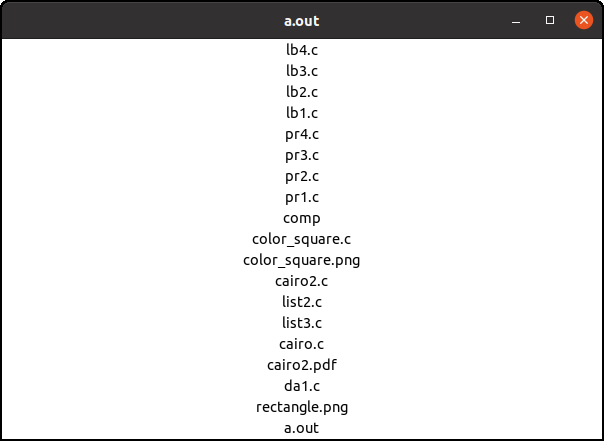
\includegraphics[width=10cm,height=7.3cm]{../image/list3.png}
\caption{screenshot list3}
\end{figure}

  \hypertarget{gtkgridview-and-activate-signal}{%
\section{GtkGridView and activate
signal}\label{gtkgridview-and-activate-signal}}

GtkGridView is similar to GtkListView. It displays a GListModel as a
grid, which is like a square tessellation.

\begin{figure}
\centering
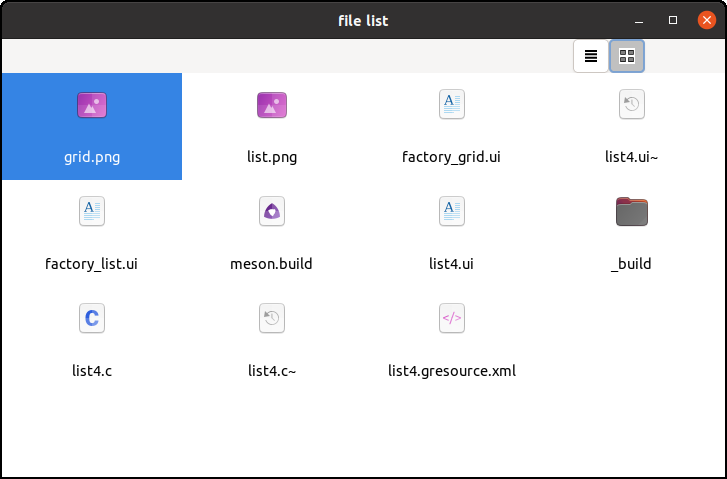
\includegraphics[width=10cm,height=6.6cm]{../image/list4.png}
\caption{Grid}
\end{figure}

This is often seen when you use a file browser like nautilus.

In this section, let's make a very simple file browser
\passthrough{\lstinline!list4!}. It just shows the files in the current
directory. And a user can choose list or grid by clicking on buttons in
the tool bar. Each item in the list or grid has an icon and a filename.
In addition, \passthrough{\lstinline!list4!} provides the way to open
the \passthrough{\lstinline!tfe!} text editor to show a text file. A
user can do that by double clicking on an item or pressing enter key
when an item is selected.

\hypertarget{gtkdirectorylist}{%
\subsection{GtkDirectoryList}\label{gtkdirectorylist}}

GtkDirectoryList implements GListModel and it contains information of
files in a certain directory. The items of the list are GFileInfo
objects.

In the \passthrough{\lstinline!list4!} source files, GtkDirectoryList is
described in a ui file and built by GtkBuilder. The GtkDirectoryList
instance is assigned to the ``model'' property of a GtkSingleSelection
instance. And the GtkSingleSelection instance is assigned to the
``model'' property of a GListView or GGridView instance.

\begin{lstlisting}
GtkListView (model property) => GtkSingleSelection (model property) => GtkDirectoryList
GtkGridView (model property) => GtkSingleSelection (model property) => GtkDirectoryList
\end{lstlisting}

\begin{figure}
\centering
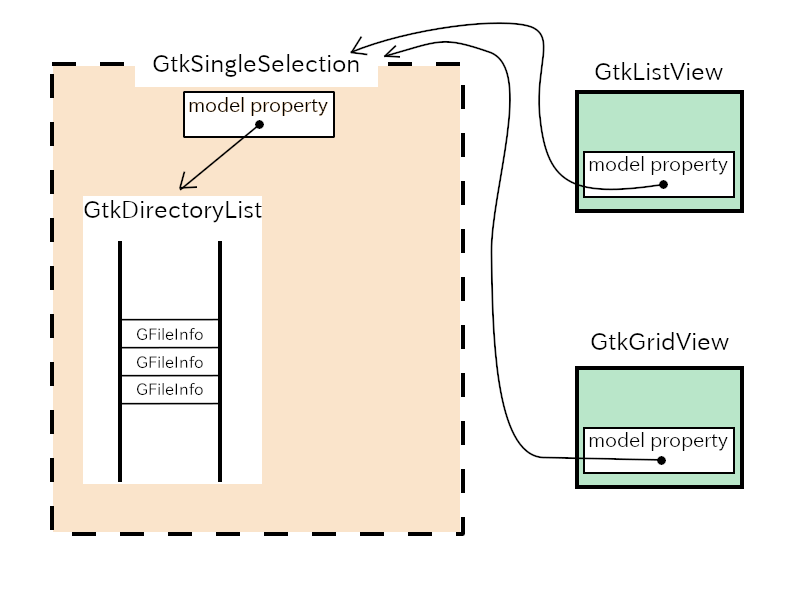
\includegraphics[width=10cm,height=7.5cm]{../image/directorylist.png}
\caption{DirectoryList}
\end{figure}

The following is the part of the ui file
\passthrough{\lstinline!list4.ui!}. It defines GtkListView,
GtkSingleSelection and GtkDirectoryList. It also defines GtkGridView and
GtkSingleSelection.

\begin{lstlisting}[language=XML]
<object class="GtkListView" id="list">
  <property name="model">
    <object class="GtkSingleSelection" id="singleselection">
      <property name="model">
        <object class="GtkDirectoryList" id="directorylist">
          <property name="attributes">standard::name,standard::icon,standard::content-type</property>
        </object>
      </property>
    </object>
  </property>
</object>
<object class="GtkGridView" id="grid">
  <property name="model">singleselection</property>
</object>
\end{lstlisting}

GtkDirectoryList has an ``attributes'' property. It is attributes of
GFileInfo such as ``standard::name'', ``standard::icon'' and
``standard::content-type''.

\begin{itemize}
\tightlist
\item
  standard::name is a filename.
\item
  standard::icon is an icon of the file. It is a GIcon object.
\item
  standard::content-type is a content-type. Content-type is the same as
  mime type for the internet technology. For example, ``text/plain'' is
  a text file, ``text/x-csrc'' is a C source code and so on.
  (``text/x-csrc''is not registered to IANA media types. Such ``x-''
  subtype is not a standard mime type.) Content type is also used by the
  desktop system.
\end{itemize}

GtkGridView has the same structure as GtkListView. But it is enough to
specify its model property to \passthrough{\lstinline!singleselection!}
which is the identification of the GtkSingleSelection. Therefore the
description for GtkGridView is very short.

\hypertarget{ui-file-of-the-window}{%
\subsection{Ui file of the window}\label{ui-file-of-the-window}}

Look at the screenshot of \passthrough{\lstinline!list4!} at the top of
this section. The widgets are built with the following ui file.

\begin{lstlisting}[language=XML, numbers=left]
<?xml version="1.0" encoding="UTF-8"?>
<interface>
  <object class="GtkApplicationWindow" id="win">
    <property name="title">file list</property>
    <property name="default-width">600</property>
    <property name="default-height">400</property>
    <child>
      <object class="GtkBox" id="boxv">
        <property name="orientation">GTK_ORIENTATION_VERTICAL</property>
        <child>
          <object class="GtkBox" id="boxh">
            <property name="orientation">GTK_ORIENTATION_HORIZONTAL</property>
            <child>
              <object class="GtkLabel" id="dmy1">
                <property name="hexpand">TRUE</property>
              </object>
            </child>
            <child>
              <object class="GtkButton" id="btnlist">
                <property name="name">btnlist</property>
                <property name="action-name">win.view</property>
                <property name="action-target">&apos;list&apos;</property>
                <child>
                  <object class="GtkImage">
                    <property name="resource">/com/github/ToshioCP/list4/list.png</property>
                  </object>
                </child>
              </object>
            </child>
            <child>
              <object class="GtkButton" id="btngrid">
                <property name="name">btngrid</property>
                <property name="action-name">win.view</property>
                <property name="action-target">&apos;grid&apos;</property>
                <child>
                  <object class="GtkImage">
                    <property name="resource">/com/github/ToshioCP/list4/grid.png</property>
                  </object>
                </child>
              </object>
            </child>
            <child>
              <object class="GtkLabel" id="dmy2">
                <property name="width-chars">10</property>
              </object>
            </child>
          </object>
        </child>
        <child>
          <object class="GtkScrolledWindow" id="scr">
            <property name="hexpand">TRUE</property>
            <property name="vexpand">TRUE</property>
          </object>
        </child>
      </object>
    </child>
  </object>
  <object class="GtkListView" id="list">
    <property name="model">
      <object class="GtkSingleSelection" id="singleselection">
        <property name="model">
          <object class="GtkDirectoryList" id="directorylist">
            <property name="attributes">standard::name,standard::icon,standard::content-type</property>
          </object>
        </property>
      </object>
    </property>
  </object>
  <object class="GtkGridView" id="grid">
    <property name="model">singleselection</property>
  </object>
</interface>
\end{lstlisting}

The file consists of two parts. The first part begins at the third line
and ends at the 57th line. This part is the widgets from the top level
window to the scrolled window. It also includes two buttons. The second
part begins at the 58th line and ends at the 71st line. This is the part
of GtkListView and GtkGridView. They are described in the previous
section.

\begin{itemize}
\tightlist
\item
  13-17, 42-46: Two labels are dummy labels. They just work as a space
  to put the two buttons at the appropriate position.
\item
  19-41: GtkButton \passthrough{\lstinline!btnlist!} and
  \passthrough{\lstinline!btngrid!}. These two buttons work as selection
  buttons to switch from list to grid and vice versa. These two buttons
  are connected to a stateful action \passthrough{\lstinline!win.view!}.
  This action is stateful and has a parameter. Such action consists of
  prefix, action name and parameter. The prefix of the action is
  \passthrough{\lstinline!win!}, which means the action belongs to the
  top level window. So, a prefix gives the scope of the action. The
  action name is \passthrough{\lstinline!view!}. The parameters are
  \passthrough{\lstinline!list!} or \passthrough{\lstinline!grid!},
  which show the state of the action. A parameter is also called a
  target, because it is a target to which the buttons are clicked on to
  change the action state. We often write the detailed action like
  ``win.view::list'' or ``win.view::grid''.
\item
  21-22: The properties ``action-name'' and ``action-target'' belong to
  GtkActionable interface. GtkButton implements GtkActionable. The
  action name is ``win.view'' and the target is ``list''. Generally, a
  target is GVariant, which can be string, integer, float and so on. You
  need to use GVariant text format to write GVariant value in ui files.
  If the type of the GVariant value is string, then the value with
  GVariant text format is bounded by single quotes or double quotes.
  Because ui file is xml format text, single quote cannot be written
  without escape. Its escape sequence is \&apos;. Therefore, the target
  `list' is written as \&apos;list\&apos;. Because the button is
  connected to the action, ``clicked'' signal handler isn't needed.
\item
  23-27: The child widget of the button is GtkImage. GtkImage has a
  ``resource'' property. It is a GResource and GtkImage reads an image
  data from the resource and sets the image. This resource is built from
  24x24-sized png image data, which is an original icon.
\item
  50-53: GtkScrolledWindow. Its child widget will be GtkListView or
  GtkGridView.
\end{itemize}

The action \passthrough{\lstinline!view!} is created, connected to the
``activate'' signal handler and inserted to the window (action map) as
follows.

\begin{lstlisting}[language=C]
  act_view = g_simple_action_new_stateful ("view", g_variant_type_new("s"), g_variant_new_string ("list"));
  g_signal_connect (act_view, "activate", G_CALLBACK (view_activated), scr); /* scr is the GtkScrolledWindow object */
  g_action_map_add_action (G_ACTION_MAP (win), G_ACTION (act_view));
\end{lstlisting}

The signal handler \passthrough{\lstinline!view\_activated!} will be
explained later.

\hypertarget{factories}{%
\subsection{Factories}\label{factories}}

Each view (GtkListView and GtkGridView) has its own factory because its
items have different structure of widgets. The factories are
GtkBuilderListItemFactory objects. Their ui files are as follows.

factory\_list.ui

\begin{lstlisting}[language=XML, numbers=left]
<?xml version="1.0" encoding="UTF-8"?>
<interface>
  <template class="GtkListItem">
    <property name="child">
      <object class="GtkBox">
        <property name="orientation">GTK_ORIENTATION_HORIZONTAL</property>
        <property name="spacing">20</property>
        <child>
          <object class="GtkImage">
            <binding name="gicon">
              <closure type="GIcon" function="get_icon">
                <lookup name="item">GtkListItem</lookup>
              </closure>
            </binding>
          </object>
        </child>
        <child>
          <object class="GtkLabel">
            <property name="hexpand">TRUE</property>
            <property name="xalign">0</property>
            <binding name="label">
              <closure type="gchararray" function="get_file_name">
                <lookup name="item">GtkListItem</lookup>
              </closure>
            </binding>
          </object>
        </child>
      </object>
    </property>
  </template>
</interface>
\end{lstlisting}

factory\_grid.ui

\begin{lstlisting}[language=XML, numbers=left]
<?xml version="1.0" encoding="UTF-8"?>
<interface>
  <template class="GtkListItem">
    <property name="child">
      <object class="GtkBox">
        <property name="orientation">GTK_ORIENTATION_VERTICAL</property>
        <property name="spacing">20</property>
        <child>
          <object class="GtkImage">
            <property name="icon-size">GTK_ICON_SIZE_LARGE</property>
            <binding name="gicon">
              <closure type="GIcon" function="get_icon">
                <lookup name="item">GtkListItem</lookup>
              </closure>
            </binding>
          </object>
        </child>
        <child>
          <object class="GtkLabel">
            <property name="hexpand">TRUE</property>
            <property name="xalign">0.5</property>
            <binding name="label">
              <closure type="gchararray" function="get_file_name">
                <lookup name="item">GtkListItem</lookup>
              </closure>
            </binding>
          </object>
        </child>
      </object>
    </property>
  </template>
</interface>
\end{lstlisting}

The two files above are almost same. The difference is:

\begin{itemize}
\tightlist
\item
  The orientation of the box
\item
  The icon size
\item
  The position of the text of the label
\end{itemize}

\begin{lstlisting}
$ cd list4; diff factory_list.ui factory_grid.ui
6c6
<         <property name="orientation">GTK_ORIENTATION_HORIZONTAL</property>
---
>         <property name="orientation">GTK_ORIENTATION_VERTICAL</property>
9a10
>             <property name="icon-size">GTK_ICON_SIZE_LARGE</property>
20c21
<             <property name="xalign">0</property>
---
>             <property name="xalign">0.5</property>
\end{lstlisting}

Each view item has two properties, ``gicon'' property of GtkImage and
``label'' property of GtkLabel. Because GFileInfo doesn't have
properties correspond to icon or filename, the factory uses closure tag
to bind ``gicon'' and ``label'' properties to GFileInfo information. A
function \passthrough{\lstinline!get\_icon!} gets GIcon the GFileInfo
object has. And a function \passthrough{\lstinline!get\_file\_name!}
gets a filename the GFileInfo object has.

\begin{lstlisting}[language=C, numbers=left]
GIcon *
get_icon (GtkListItem *item, GFileInfo *info) {
  GIcon *icon;

  if (! G_IS_FILE_INFO (info))
    return NULL;
  else {
    icon = g_file_info_get_icon (info);
    g_object_ref (icon);
    return icon;
  }
}

char *
get_file_name (GtkListItem *item, GFileInfo *info) {
  if (! G_IS_FILE_INFO (info))
    return NULL;
  else
    return g_strdup (g_file_info_get_name (info));
}
\end{lstlisting}

One important thing is view items own the instance or string. It is
achieved by \passthrough{\lstinline!g\_object\_ref!} to increase the
reference count by one, or \passthrough{\lstinline!strdup!} to create a
copy of the string. The object or string will be automatically freed in
unbinding process when the view item is recycled.

\hypertarget{an-activate-signal-handler-of-the-action}{%
\subsection{An activate signal handler of the
action}\label{an-activate-signal-handler-of-the-action}}

An activate signal handler \passthrough{\lstinline!view\_activate!}
switches the view. It does two things.

\begin{itemize}
\tightlist
\item
  Changes the child widget of GtkScrolledWindow.
\item
  Changes the CSS of buttons to show the current state.
\end{itemize}

\begin{lstlisting}[language=C, numbers=left]
static void
view_activated(GSimpleAction *action, GVariant *parameter, gpointer user_data) {
  GtkScrolledWindow *scr = GTK_SCROLLED_WINDOW (user_data);
  const char *view = g_variant_get_string (parameter, NULL);
  const char *other;
  char *css;

  if (strcmp (view, "list") == 0) {
    other = "grid";
    gtk_scrolled_window_set_child (scr, list);
  }else {
    other = "list";
    gtk_scrolled_window_set_child (scr, grid);
  }
  css = g_strdup_printf ("button#btn%s {background: silver;} button#btn%s {background: white;}", view, other);
  gtk_css_provider_load_from_data (provider, css, -1);
  g_free (css);
  g_action_change_state (G_ACTION (action), parameter);
}
\end{lstlisting}

The second parameter of this handler is the target of the clicked
button. Its type is GVariant.

\begin{itemize}
\tightlist
\item
  If \passthrough{\lstinline!btnlist!} has been clicked, then
  \passthrough{\lstinline!parameter!} is a GVariant of the string
  ``list''.
\item
  If \passthrough{\lstinline!btngrid!} has been clicked, then
  \passthrough{\lstinline!parameter!} is a GVariant of the string
  ``grid''.
\end{itemize}

The third parameter \passthrough{\lstinline!user\_data!} points
GtkScrolledWindow, which is set in the
\passthrough{\lstinline!g\_signal\_connect!} function.

\begin{itemize}
\tightlist
\item
  4: \passthrough{\lstinline!g\_variant\_get\_string!} gets the string
  from the GVariant variable.
\item
  8-14: Sets the child of \passthrough{\lstinline!scr!}. The function
  \passthrough{\lstinline!gtk\_scrolled\_window\_set\_child!} decreases
  the reference count of the old child by one. And it increases the
  reference count of the new child by one.
\item
  15-17: Sets the CSS of the buttons. The background of the clicked
  button will be silver color and the other button will be white.
\item
  18: Changes the state of the action.
\end{itemize}

\hypertarget{activate-signal-of-gtklistview-and-gtkgridview}{%
\subsection{Activate signal of GtkListView and
GtkGridView}\label{activate-signal-of-gtklistview-and-gtkgridview}}

Views (GtkListView and GtkGridView) have an ``activate'' signal. It is
emitted when an item in the view is double clicked or the enter key is
pressed. You can do anything you like by connecting the ``activate''
signal to the handler.

The example \passthrough{\lstinline!list4!} launches
\passthrough{\lstinline!tfe!} text file editor if the item of the list
is a text file.

\begin{lstlisting}[language=C]
static void
list_activate (GtkListView *list, int position, gpointer user_data) {
  GFileInfo *info = G_FILE_INFO (g_list_model_get_item (G_LIST_MODEL (gtk_list_view_get_model (list)), position));
  launch_tfe_with_file (info);
}

static void
grid_activate (GtkGridView *grid, int position, gpointer user_data) {
  GFileInfo *info = G_FILE_INFO (g_list_model_get_item (G_LIST_MODEL (gtk_grid_view_get_model (grid)), position));
  launch_tfe_with_file (info);
}

... ...
... ...

  g_signal_connect (GTK_LIST_VIEW (list), "activate", G_CALLBACK (list_activate), NULL);
  g_signal_connect (GTK_GRID_VIEW (grid), "activate", G_CALLBACK (grid_activate), NULL);
\end{lstlisting}

The second parameter of the handlers is the position of the item
(GFileInfo) of the GListModel. So you can get the item with
\passthrough{\lstinline!g\_list\_model\_get\_item!} function.

\hypertarget{content-type-and-launching-an-application}{%
\subsection{Content type and launching an
application}\label{content-type-and-launching-an-application}}

The function \passthrough{\lstinline!launch\_tfe\_with\_file!} gets a
file from the GFileInfo instance. If the file is a text file, it
launches \passthrough{\lstinline!tfe!} with the file.

GFileInfo has information about file type. The file type is like
``text/plain'', ``text/x-csrc'' and so on. It is called content type.
Content type can be got with
\passthrough{\lstinline!g\_file\_info\_get\_content\_type!} function.

\begin{lstlisting}[language=C, numbers=left]
static void
launch_tfe_with_file (GFileInfo *info) {
  GError *err = NULL;
  GFile *file;
  GList *files = NULL;
  const char *content_type;
  const char *text_type = "text/";
  GAppInfo *appinfo;
  int i;

  if (! info)
    return;
  content_type = g_file_info_get_content_type (info);
g_print ("%s\n", content_type);  /* This line can be commented out if unnecessary */
  if (! content_type)
    return;
  for (i=0;i<5;++i) {
    if (content_type[i] != text_type[i])
      return;
  }
  appinfo = g_app_info_create_from_commandline ("tfe", "tfe", G_APP_INFO_CREATE_NONE, &err);
  if (err) {
    g_printerr ("%s\n", err->message);
    g_error_free (err);
    return;
  }
  err = NULL;
  file = g_file_new_for_path (g_file_info_get_name (info));
  files = g_list_append (files, file);
  if (! (g_app_info_launch (appinfo, files, NULL, &err))) {
    g_printerr ("%s\n", err->message);
    g_error_free (err);
  }
  g_list_free_full (files, g_object_unref);
  g_object_unref (appinfo);
}
\end{lstlisting}

\begin{itemize}
\tightlist
\item
  13: Gets the content type of the file from GFileInfo.
\item
  14: Prints the content type. This is only useful to know a content
  type of a file. You can delete it if unnecessary.
\item
  17-20: If the content type doesn't begin with ``text/'', then it
  returns.
\item
  21: Creates GAppInfo object of \passthrough{\lstinline!tfe!}
  application. GAppInfo is an interface and the variable
  \passthrough{\lstinline!appinfo!} points a GDesktopAppInfo instance.
  GAppInfo is a collection of information of an application.
\item
  30: Launches the application (\passthrough{\lstinline!tfe!}) with an
  argument \passthrough{\lstinline!file!}.
  \passthrough{\lstinline!g\_app\_info\_launch!} has four parameters.
  The first parameter is GAppInfo object. The second parameter is a list
  of GFile objects. In this function, only one GFile instance is given
  to \passthrough{\lstinline!tfe!}, but you can give more arguments. The
  third parameter is GAppLaunchContext, but this program gives NULL
  instead. The last parameter is the pointer to the pointer to a GError.
\item
  34: \passthrough{\lstinline!g\_list\_free\_full!} frees the memories
  used by the list and items.
\end{itemize}

If your distribution supports Gtk4, using
\passthrough{\lstinline!g\_app\_info\_launch\_default\_for\_uri!} is
convenient. The function automatically determines the default
application from the file and launches it. For example, if the file is
text, then it launches gedit with the file. Such functionality comes
from desktop.

\hypertarget{compilation-and-execution}{%
\subsection{Compilation and execution}\label{compilation-and-execution}}

The source files are located in src/list4 directory. To compile and
execute list4, type as follows.

\begin{lstlisting}
$ cd list4 # or cd src/list4. It depends your current directory.
$ meson _build
$ ninja -C _build
$ _build/list4
\end{lstlisting}

Then a file list appears as a list style. Click on a button on the tool
bar so that you can change the style to grid or back to list. Double
click ``list4.c'' item, then \passthrough{\lstinline!tfe!} text editor
runs with the argument ``list4.c''. The following is the screenshot.

\begin{figure}
\centering
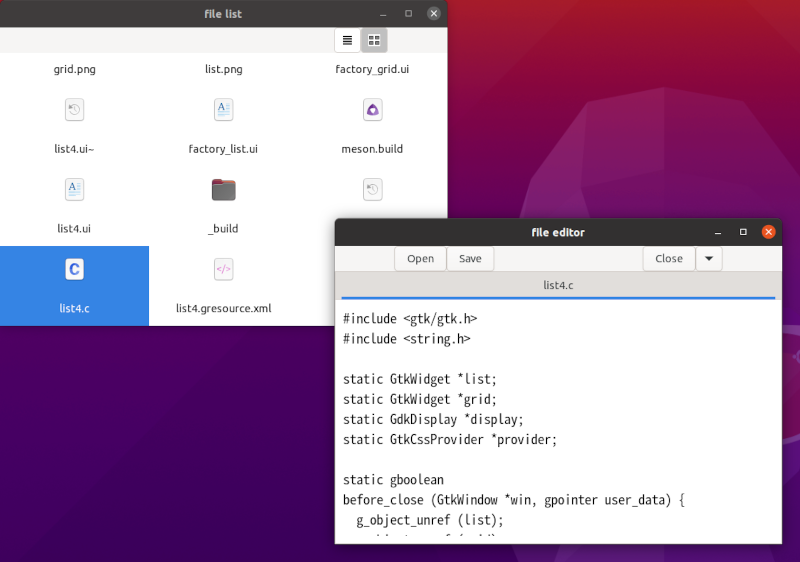
\includegraphics[width=8cm,height=5.62cm]{../image/screenshot_list4.png}
\caption{Screenshot}
\end{figure}

\hypertarget{gbytes-property-of-gtkbuilderlistitemfactory}{%
\subsection{``gbytes'' property of
GtkBuilderListItemFactory}\label{gbytes-property-of-gtkbuilderlistitemfactory}}

GtkBuilderListItemFactory has ``gbytes'' property. The property contains
a byte sequence of ui data. If you use this property, you can put the
contents of \passthrough{\lstinline!factory\_list.ui!} and
\passthrough{\lstinline!factory\_grid.ui!}into
\passthrough{\lstinline!list4.ui!}. The following shows a part of the
new ui file (\passthrough{\lstinline!list5.ui!}).

\begin{lstlisting}[language=XML]
  <object class="GtkListView" id="list">
    <property name="model">
      <object class="GtkSingleSelection" id="singleselection">
        <property name="model">
          <object class="GtkDirectoryList" id="directorylist">
            <property name="attributes">standard::name,standard::icon,standard::content-type</property>
          </object>
        </property>
      </object>
    </property>
    <property name="factory">
      <object class="GtkBuilderListItemFactory">
        <property name="bytes"><![CDATA[
<?xml version="1.0" encoding="UTF-8"?>
<interface>
  <template class="GtkListItem">
    <property name="child">
      <object class="GtkBox">
        <property name="orientation">GTK_ORIENTATION_HORIZONTAL</property>
        <property name="spacing">20</property>
        <child>
          <object class="GtkImage">
            <binding name="gicon">
              <closure type="GIcon" function="get_icon">
                <lookup name="item">GtkListItem</lookup>
              </closure>
            </binding>
          </object>
        </child>
        <child>
          <object class="GtkLabel">
            <property name="hexpand">TRUE</property>
            <property name="xalign">0</property>
            <binding name="label">
              <closure type="gchararray" function="get_file_name">
                <lookup name="item">GtkListItem</lookup>
              </closure>
            </binding>
          </object>
        </child>
      </object>
    </property>
  </template>
</interface>
        ]]></property>
      </object>
    </property>
  </object>
\end{lstlisting}

CDATA section begins with ``\textless{[}CDATA{[}" and ends with
"{]}{]}\textgreater{}''. The contents of CDATA section is recognized as
a string. Any character, even if it is a key syntax marker such as
`\textless{}' or `\textgreater{}', is recognized literally. Therefore,
the text between ``\textless{[}CDATA{[}" and "{]}{]}\textgreater{}'' is
inserted to ``bytes'' property as it is.

This method decreases the number of ui files. But, the new ui file is a
bit complicated especially for the beginners. If you feel some
difficulty, it is better for you to separate the ui file.

A directory src/list5 includes the ui file above.

  \hypertarget{gtkexpression}{%
\section{GtkExpression}\label{gtkexpression}}

GtkExpression is a fundamental type. It is not a descendant of GObject.
GtkExpression provides a way to describe references to values.
GtkExpression needs to be evaluated to obtain a value.

It is similar to arithmetic calculation.

\begin{lstlisting}
1 + 2 = 3
\end{lstlisting}

\passthrough{\lstinline!1+2!} is an expression. It shows the way how to
calculate. \passthrough{\lstinline!3!} is the value comes from the
expression. Evaluation is to calculate the expression and get the value.

GtkExpression is a way to get a value. Evaluation is like a calculation.
A value is got by evaluating the expression.

First, I want to show you the C file of the example for GtkExpression.
Its name is \passthrough{\lstinline!exp.c!} and located under
src/expression directory. You don't need to understand the details now,
just look at it. It will be explained in the next subsection.

\begin{lstlisting}[language=C, numbers=left]
#include <gtk/gtk.h>

GtkWidget *win1;
int width, height;
GtkExpressionWatch *watch_width;
GtkExpressionWatch *watch_height;

/* Notify is called when "default-width" or "default-height" property is changed. */
static void
notify (gpointer user_data) {
  GValue value = G_VALUE_INIT;
  char *title;

  if (watch_width && gtk_expression_watch_evaluate (watch_width, &value))
    width = g_value_get_int (&value);
  g_value_unset (&value);
  if (watch_height && gtk_expression_watch_evaluate (watch_height, &value))
    height = g_value_get_int (&value);
  g_value_unset (&value);
  title = g_strdup_printf ("%d x %d", width, height);
  gtk_window_set_title (GTK_WINDOW (win1), title);
  g_free (title);
}

/* This function is used by closure tag in exp.ui. */
char *
set_title (GtkWidget *win, int width, int height) {
  return g_strdup_printf ("%d x %d", width, height);
}

/* ----- activate, open, startup handlers ----- */
static void
app_activate (GApplication *application) {
  GtkApplication *app = GTK_APPLICATION (application);
  GtkWidget *box;
  GtkWidget *label1, *label2, *label3;
  GtkWidget *entry;
  GtkEntryBuffer *buffer;
  GtkBuilder *build;
  GtkExpression *expression, *expression1, *expression2;
  GValue value = G_VALUE_INIT;
  char *s;

  /* Creates GtkApplicationWindow instance. */
  /* The codes below are complecated. It does the same as "win1 = gtk_application_window_new (app);". */
  /* The codes are written just to show how to use GtkExpression. */
  expression = gtk_cclosure_expression_new (GTK_TYPE_APPLICATION_WINDOW, NULL, 0, NULL,
                 G_CALLBACK (gtk_application_window_new), NULL, NULL);
  if (gtk_expression_evaluate (expression, app, &value)) {
    win1 = GTK_WIDGET (g_value_get_object (&value)); /* GtkApplicationWindow */
    g_object_ref (win1);
    g_print ("Got GtkApplicationWindow instance.\n");
  }else
    g_print ("The cclosure expression wasn't evaluated correctly.\n");
  gtk_expression_unref (expression);
  g_value_unset (&value);    /* At the same time, the reference count of win1 is decreased by one. */

  /* Builds a window with components */
  box = gtk_box_new (GTK_ORIENTATION_VERTICAL, 10);
  label1 = gtk_label_new (NULL);
  label2 = gtk_label_new (NULL);
  label3 = gtk_label_new (NULL);
  buffer = gtk_entry_buffer_new (NULL, 0);
  entry = gtk_entry_new_with_buffer (buffer);
  gtk_box_append (GTK_BOX (box), label1);
  gtk_box_append (GTK_BOX (box), label2);
  gtk_box_append (GTK_BOX (box), label3);
  gtk_box_append (GTK_BOX (box), entry);
  gtk_window_set_child (GTK_WINDOW (win1), box);

  /* Constant expression */
  expression = gtk_constant_expression_new (G_TYPE_INT,100);
  if (gtk_expression_evaluate (expression, NULL, &value)) {
    s = g_strdup_printf ("%d", g_value_get_int (&value));
    gtk_label_set_text (GTK_LABEL (label1), s);
    g_free (s);
  } else
    g_print ("The constant expression wasn't evaluated correctly.\n");
  gtk_expression_unref (expression);
  g_value_unset (&value);

  /* Property expression and binding*/
  expression1 = gtk_property_expression_new (GTK_TYPE_ENTRY, NULL, "buffer");
  expression2 = gtk_property_expression_new (GTK_TYPE_ENTRY_BUFFER, expression1, "text");
  gtk_expression_bind (expression2, label2, "label", entry);

  /* Constant expression instead of "this" instance */
  expression1 = gtk_constant_expression_new (GTK_TYPE_APPLICATION, app);
  expression2 = gtk_property_expression_new (GTK_TYPE_APPLICATION, expression1, "application-id");
  if (gtk_expression_evaluate (expression2, NULL, &value))
    gtk_label_set_text (GTK_LABEL (label3), g_value_get_string (&value));
  else
    g_print ("The property expression wasn't evaluated correctly.\n");
  gtk_expression_unref (expression1); /* expression 2 is also freed. */
  g_value_unset (&value);

  width = 800;
  height = 600;
  gtk_window_set_default_size (GTK_WINDOW (win1), width, height);
  notify(NULL);

  /* GtkExpressionWatch */
  expression1 = gtk_property_expression_new (GTK_TYPE_WINDOW, NULL, "default-width");
  watch_width = gtk_expression_watch (expression1, win1, notify, NULL, NULL);
  expression2 = gtk_property_expression_new (GTK_TYPE_WINDOW, NULL, "default-height");
  watch_height = gtk_expression_watch (expression2, win1, notify, NULL, NULL);

  gtk_widget_show (win1);

  /* Builds a window with exp.ui resource */
  build = gtk_builder_new_from_resource ("/com/github/ToshioCP/exp/exp.ui");
  GtkWidget *win2 = GTK_WIDGET (gtk_builder_get_object (build, "win2"));
  gtk_window_set_application (GTK_WINDOW (win2), app);
  g_object_unref (build);

  gtk_widget_show (win2);
}

static void
app_startup (GApplication *application) {
}

#define APPLICATION_ID "com.github.ToshioCP.exp"

int
main (int argc, char **argv) {
  GtkApplication *app;
  int stat;

  app = gtk_application_new (APPLICATION_ID, G_APPLICATION_FLAGS_NONE);

  g_signal_connect (app, "startup", G_CALLBACK (app_startup), NULL);
  g_signal_connect (app, "activate", G_CALLBACK (app_activate), NULL);
/*  g_signal_connect (app, "open", G_CALLBACK (app_open), NULL);*/

  stat =g_application_run (G_APPLICATION (app), argc, argv);
  g_object_unref (app);
  return stat;
}
\end{lstlisting}

\passthrough{\lstinline!exp.c!} consists of five functions.

\begin{itemize}
\tightlist
\item
  \passthrough{\lstinline!notify!}
\item
  \passthrough{\lstinline!set\_title!}
\item
  \passthrough{\lstinline!app\_activate!}. This is a handler of
  ``activate'' signal on GtkApplication instance.
\item
  \passthrough{\lstinline!app\_startup!}. This is a handler of
  ``startup''signal. But nothing is done in this function.
\item
  \passthrough{\lstinline!main!}.
\end{itemize}

The function \passthrough{\lstinline!app\_activate!} is an actual main
body in \passthrough{\lstinline!exp.c!}.

\hypertarget{constant-expression}{%
\subsection{Constant expression}\label{constant-expression}}

Constant expression provides constant value or instance when it is
evaluated.

\begin{itemize}
\tightlist
\item
  72-80: A constant expression. It is extracted and put into here.
\end{itemize}

\begin{lstlisting}[language=C]
  expression = gtk_constant_expression_new (G_TYPE_INT,100);
  if (gtk_expression_evaluate (expression, NULL, &value)) {
    s = g_strdup_printf ("%d", g_value_get_int (&value));
    gtk_label_set_text (GTK_LABEL (label1), s);
    g_free (s);
  } else
    g_print ("The constant expression wasn't evaluated correctly.\n");
  gtk_expression_unref (expression);
  g_value_unset (&value);
\end{lstlisting}

\begin{itemize}
\tightlist
\item
  Constant expression is created with
  \passthrough{\lstinline!gtk\_constant\_expression\_new!} function. The
  parameter of the function is a type (GType) and a value (or instance).
\item
  \passthrough{\lstinline!gtk\_expression\_evaluate!} evaluates the
  expression. It has three parameters, the expression to evaluate,
  \passthrough{\lstinline!this!} instance and GValue for being set with
  the value. \passthrough{\lstinline!this!} instance isn't necessary for
  constant expressions. Therefore the second argument is NULL.
  \passthrough{\lstinline!gtk\_expression\_evaluate!} returns TRUE if it
  successfully evaluates the expression. Otherwise it returns FALSE.
\item
  If it returns TRUE, the GValue \passthrough{\lstinline!value!} is set
  with the value of the expression. The type of the value is int.
  \passthrough{\lstinline!g\_strdup\_printf!} converts the value to a
  string \passthrough{\lstinline!s!}.
\item
  GtkLabel \passthrough{\lstinline!label1!} is set with
  \passthrough{\lstinline!s!}. The string \passthrough{\lstinline!s!}
  needs to be freed.
\item
  If the evaluation fails a message is outputted to stderr.
\item
  The expression and GValue are freed.
\end{itemize}

Constant expression is usually used to give a constant value or instance
to another expression.

\hypertarget{property-expression}{%
\subsection{Property expression}\label{property-expression}}

Property expression looks up a property in a GObject object. For
example, a property expression that refers ``label'' property in
GtkLabel object is created like this.

\begin{lstlisting}[language=C]
expression = gtk_property_expression_new (GTK_TYPE_LABEL, another_expression, "label");
\end{lstlisting}

\passthrough{\lstinline!another\_expression!} is expected to give a
GtkLabel instance when it is evaluated. For example,

\begin{lstlisting}[language=C]
label = gtk_label_new ("Hello");
another_expression = gtk_constant_expression_new (GTK_TYPE_LABEL, label);
expression = gtk_property_expression_new (GTK_TYPE_LABEL, another_expression, "label");
\end{lstlisting}

If \passthrough{\lstinline!expression!} is evaluated, the second
parameter \passthrough{\lstinline!another\_expression!} is evaluated in
advance. The value of \passthrough{\lstinline!another\_expression!} is
\passthrough{\lstinline!label!} (GtkLabel instance). Then,
\passthrough{\lstinline!expression!} looks up ``label'' property of
\passthrough{\lstinline!label!} and the evaluation result is ``Hello''.

In the example above, the second argument of
\passthrough{\lstinline!gtk\_property\_expression\_new!} is another
expression. But the second argument can be NULL. If it is NULL,
\passthrough{\lstinline!this!} instance is used instead.
\passthrough{\lstinline!this!} is given by
\passthrough{\lstinline!gtk\_expression\_evaluate!} function at the
evaluation.

Now look at \passthrough{\lstinline!exp.c!}. The lines from 83 to 85 is
extracted here.

\begin{lstlisting}[language=C]
  expression1 = gtk_property_expression_new (GTK_TYPE_ENTRY, NULL, "buffer");
  expression2 = gtk_property_expression_new (GTK_TYPE_ENTRY_BUFFER, expression1, "text");
  gtk_expression_bind (expression2, label2, "label", entry);
\end{lstlisting}

\begin{itemize}
\tightlist
\item
  \passthrough{\lstinline!expression1!} looks up ``buffer'' property of
  \passthrough{\lstinline!this!} object, which is
  \passthrough{\lstinline!GTK\_TYPE\_ENTRY!} type.
\item
  \passthrough{\lstinline!expression2!} looks up ``text'' property of
  GtkEntryBuffer object given by \passthrough{\lstinline!epression1!}.
\item
  \passthrough{\lstinline!gtk\_expression\_bind!} binds a property to a
  value given by the expression. In this program, it binds a ``label''
  property in \passthrough{\lstinline!label2!} to the value evaluated
  with \passthrough{\lstinline!expresion2!} with
  \passthrough{\lstinline!entry!} as \passthrough{\lstinline!this!}
  object. The evaluation process is as follows.

  \begin{enumerate}
  \def\labelenumi{\arabic{enumi}.}
  \tightlist
  \item
    \passthrough{\lstinline!expression2!} is evaluated. But it includes
    \passthrough{\lstinline!expression1!} so
    \passthrough{\lstinline!expression1!} is evaluated in advance.
  \item
    Because the second argument of \passthrough{\lstinline!expression1!}
    is NULL, \passthrough{\lstinline!this!} object is used.
    \passthrough{\lstinline!this!} is given by
    \passthrough{\lstinline!gtk\_expression\_bind!}. It is
    \passthrough{\lstinline!entry!} (GtkEntry instance).
    \passthrough{\lstinline!expression1!} looks up ``buffer'' property
    in \passthrough{\lstinline!entry!}. It is a GtkEntryBuffer instance
    \passthrough{\lstinline!buffer!}. (See line 64 in
    \passthrough{\lstinline!exp.c!}.)
  \item
    Then, \passthrough{\lstinline!expression2!} looks up ``text''
    property in \passthrough{\lstinline!buffer!}. It is a text held in
    \passthrough{\lstinline!entry!}.
  \item
    The text is assigned to ``label'' property in
    \passthrough{\lstinline!label2!}.
  \end{enumerate}
\item
  \passthrough{\lstinline!gtk\_expression\_bind!} creates a
  GtkExpressionWatch. (But it isn't assigned to a variable in the
  program above. If you want to keep the GtkExpressionWatch instance,
  assign it to a variable.)
\end{itemize}

\begin{lstlisting}[language=C]
  GtkExpressionWatch *watch;
  watch = gtk_expression_bind (expression2, label2, "label", entry);
\end{lstlisting}

\begin{itemize}
\tightlist
\item
  Whenever the value from \passthrough{\lstinline!expression2!} changes,
  it evaluates \passthrough{\lstinline!expression2!} and set ``label''
  property in \passthrough{\lstinline!label2!}. So, the change of the
  text in \passthrough{\lstinline!entry!} makes the ``label'' property
  reflect it immediately.
\end{itemize}

\hypertarget{closure-expression}{%
\subsection{Closure expression}\label{closure-expression}}

Closure expression calls closure when it is evaluated. A closure is a
generic representation of a callback (a pointer to a function). For
information about closure, see
\href{https://docs.gtk.org/gobject/concepts.html\#the-gobject-messaging-system}{GObject
API Reference, The GObject messaging system}. A closure expression is
created with \passthrough{\lstinline!gtk\_cclosure\_expression\_new!}
function.

\begin{lstlisting}[language=C]
GtkExpression *
gtk_cclosure_expression_new (GType value_type,
                             GClosureMarshal marshal,
                             guint n_params,
                             GtkExpression **params,
                             GCallback callback_func,
                             gpointer user_data,
                             GClosureNotify user_destroy);
\end{lstlisting}

\begin{itemize}
\tightlist
\item
  \passthrough{\lstinline!value\_type!} is the type of the value when it
  is evaluated.
\item
  \passthrough{\lstinline!marshal!} is a marshaller. You can assign
  NULL. If it is NULL, then
  \passthrough{\lstinline!g\_cclosure\_marshal\_generic ()!} is used as
  a marshaller. It is a generic marshaller function implemented via
  libffi.
\item
  \passthrough{\lstinline!n\_params!} is the number of parameters.
\item
  \passthrough{\lstinline!params!} points expressions for each parameter
  of the call back function.
\item
  \passthrough{\lstinline!callback\_func!} is a callback function.
\item
  \passthrough{\lstinline!user\_data!} is user data. You can add it for
  the closure. It is like \passthrough{\lstinline!user\_data!} in
  \passthrough{\lstinline!g\_signal\_connect!}. If it is not necessary,
  assign NULL.
\item
  \passthrough{\lstinline!user\_destroy!} is a destroy notify for
  \passthrough{\lstinline!user\_data!}. It is called to destroy
  \passthrough{\lstinline!user\_data!} when it is no longer needed. If
  NULL is assigned to \passthrough{\lstinline!user\_data!}, assign NULL
  to \passthrough{\lstinline!user\_destroy!}, too.
\end{itemize}

The following is extracted from \passthrough{\lstinline!exp.c!}. It is
from line 47 to line 56.

\begin{lstlisting}[language=C]
expression = gtk_cclosure_expression_new (GTK_TYPE_APPLICATION_WINDOW, NULL, 0, NULL,
               G_CALLBACK (gtk_application_window_new), NULL, NULL);
if (gtk_expression_evaluate (expression, app, &value)) {
  win1 = GTK_WIDGET (g_value_get_object (&value)); /* GtkApplicationWindow */
  g_object_ref (win1);
  g_print ("Got GtkApplicationWindow object.\n");
}else
  g_print ("The cclosure expression wasn't evaluated correctly.\n");
gtk_expression_unref (expression);
g_value_unset (&value);    /* At the same time, the reference count of win1 is decreased by one. */
\end{lstlisting}

The callback function is
\passthrough{\lstinline!gtk\_application\_window\_new!}. This function
has one parameter which is an instance of GtkApplication. And it returns
newly created GtkApplicationWindow instance. So, the first argument is
\passthrough{\lstinline!GTK\_TYPE\_APPLICATION\_WINDOW!} which is the
type of the return value. The second argument is NULL so general
marshaller \passthrough{\lstinline!g\_cclosure\_marshal\_generic ()!}
will be used. I think assigning NULL works in most cases when you
program in C language.

The arguments given to the call back function are
\passthrough{\lstinline!this!} object and parameters which are the
fourth argument of
\passthrough{\lstinline!gtk\_cclosure\_expression\_new!}. So, the number
of arguments is \passthrough{\lstinline!n\_params + 1!}. Because
\passthrough{\lstinline!gtk\_application\_window\_new!} has one
parameter, so \passthrough{\lstinline!n\_params!} is zero and
\passthrough{\lstinline!**params!} is NULL. No user data is necessary,
so \passthrough{\lstinline!user\_data!} and
\passthrough{\lstinline!user\_destroy!} are NULL.

\passthrough{\lstinline!gtk\_expression\_evaluate!} evaluates the
expression. \passthrough{\lstinline!this!} instance will be the first
argument for \passthrough{\lstinline!gtk\_application\_window\_new!}, so
it is \passthrough{\lstinline!app!}.

If the evaluation succeeds, the GValue \passthrough{\lstinline!value!}
holds a newly created GtkApplicationWindow instance. It is assigned to
\passthrough{\lstinline!win1!}. The GValue will be unset when it is no
longer used. And when it is unset, the GtkApplicationWindow instance
will be released and its reference count will be decreased by one. It is
necessary to increase the reference count by one in advance to keep the
instance. \passthrough{\lstinline!gtk\_expression\_unref!} frees
\passthrough{\lstinline!expression!} and \passthrough{\lstinline!value!}
is unset.

As a result, we got a GtkApplicationWindow instance
\passthrough{\lstinline!win1!}. We can do the same by:

\begin{lstlisting}[language=C]
win1 = gtk_application_window_new (app);
\end{lstlisting}

The example is more complicated and not practical than this one line
code. The aim of the example is just to show how closure expression
works.

Closure expression is flexible than other type of expression because you
can specify your own callback function.

\hypertarget{gtkexpressionwatch}{%
\subsection{GtkExpressionWatch}\label{gtkexpressionwatch}}

GtkExpressionWatch watches an expression and if the value of the
expression changes it calls its notify handler.

The example uses GtkExpressionWatch in the line 103 to 106.

\begin{lstlisting}[language=C]
expression1 = gtk_property_expression_new (GTK_TYPE_WINDOW, NULL, "default-width");
watch_width = gtk_expression_watch (expression1, win1, notify, NULL, NULL);
expression2 = gtk_property_expression_new (GTK_TYPE_WINDOW, NULL, "default-height");
watch_height = gtk_expression_watch (expression2, win1, notify, NULL, NULL);
\end{lstlisting}

The expressions above refer to ``default-width'' and ``default-height''
properties of GtkWindow. The variable
\passthrough{\lstinline!watch\_width!} watches
\passthrough{\lstinline!expression1!}. The second argument
\passthrough{\lstinline!win1!} is \passthrough{\lstinline!this!}
instance for \passthrough{\lstinline!expression1!}. So,
\passthrough{\lstinline!watch\_width!} watches the value of
``default-width'' property of \passthrough{\lstinline!win1!}. If the
value changes, it calls \passthrough{\lstinline!notify!} handler. The
fourth and fifth arguments are NULL because no user data is necessary.

The variable \passthrough{\lstinline!watch\_height!} connects
\passthrough{\lstinline!notify!} handler to
\passthrough{\lstinline!expression2!}. So,
\passthrough{\lstinline!notiry!} is also called when ``default-height''
changes.

The handler \passthrough{\lstinline!norify!} is as follows.

\begin{lstlisting}[language=C, numbers=left]
static void
notify (gpointer user_data) {
  GValue value = G_VALUE_INIT;
  char *title;

  if (watch_width && gtk_expression_watch_evaluate (watch_width, &value))
    width = g_value_get_int (&value);
  g_value_unset (&value);
  if (watch_height && gtk_expression_watch_evaluate (watch_height, &value))
    height = g_value_get_int (&value);
  g_value_unset (&value);
  title = g_strdup_printf ("%d x %d", width, height);
  gtk_window_set_title (GTK_WINDOW (win1), title);
  g_free (title);
}
\end{lstlisting}

\begin{itemize}
\tightlist
\item
  6-11: Evaluates \passthrough{\lstinline!expression1!} and
  \passthrough{\lstinline!expression2!} with
  \passthrough{\lstinline!expression\_watch\_evaluate!} function.
\item
  12: Creates a string \passthrough{\lstinline!title!}. It contains the
  width and height, for example, ``800 x 600''.
\item
  13: Sets the title of \passthrough{\lstinline!win1!} with the string
  \passthrough{\lstinline!title!}.
\end{itemize}

The title of the window reflects the size of the window.

\hypertarget{exp.ui}{%
\subsection{exp.ui}\label{exp.ui}}

\passthrough{\lstinline!exp.c!} builds a GtkWindow instance
\passthrough{\lstinline!win2!} with \passthrough{\lstinline!exp.ui!}.
The ui file \passthrough{\lstinline!exp.ui!} includes tags to create
GtkExpressions. The tags are:

\begin{itemize}
\tightlist
\item
  constant tag to create constant expression
\item
  lookup tag to create property expression
\item
  closure tag to create closure expression
\item
  binding tag to bind a property to an expression
\end{itemize}

The window \passthrough{\lstinline!win2!} behaves like
\passthrough{\lstinline!win1!}. Because similar expressions are built
with the ui file.

\begin{lstlisting}[language=XML, numbers=left]
<?xml version="1.0" encoding="UTF-8"?>
<interface>
  <object class="GtkWindow" id="win2">
    <binding name="title">
      <closure type="gchararray" function="set_title">
        <lookup name="default-width" type="GtkWindow"></lookup>
        <lookup name="default-height" type="GtkWindow"></lookup>
      </closure>
    </binding>
    <property name="default-width">600</property>
    <property name="default-height">400</property>
    <child>
      <object class="GtkBox">
        <property name="orientation">GTK_ORIENTATION_VERTICAL</property>
        <child>
          <object class="GtkLabel">
            <binding name="label">
              <constant type="gint">100</constant>
            </binding>
          </object>
        </child>
        <child>
          <object class="GtkLabel">
            <binding name="label">
              <lookup name="text">
                <lookup name="buffer">
                  entry
                </lookup>
              </lookup>
            </binding>
          </object>
        </child>
        <child>
          <object class="GtkLabel">
            <binding name="label">
              <lookup name="application-id">
                <lookup name="application">win2</lookup>
              </lookup>
            </binding>
          </object>
        </child>
        <child>
          <object class="GtkEntry" id="entry">
            <property name="buffer">
              <object class="GtkEntryBuffer"></object>
            </property>
          </object>
        </child>
      </object>
    </child>
  </object>
</interface>
\end{lstlisting}

\hypertarget{constant-tag}{%
\subsubsection{Constant tag}\label{constant-tag}}

A constant tag corresponds to a constant expression.

\begin{itemize}
\tightlist
\item
  18: Constant tag. The constant expression is created with the tag. It
  returns 100, the type is ``gint'', when it is evaluated. The type
  ``gint'' is a name of \passthrough{\lstinline!G\_TYPE\_INT!} type.
  Similarly, the types which is registered to the type system has type
  and name. For example, ``gchararray'' is a name of
  \passthrough{\lstinline!G\_TYPE\_STRING!} type. You need to use the
  name of types for the \passthrough{\lstinline!type!}attribute. See
  \href{https://github.com/ToshioCP/Gobject-tutorial/blob/main/gfm/sec5.md\#gvalue}{GObject
  tutorial}.
\item
  17-19: Binding tag corresponds to
  \passthrough{\lstinline!gtk\_expression\_bind!} function.
  \passthrough{\lstinline!name!} attribute specifies the ``label''
  property of the GtkLabel object just before the binding tag. The
  expression returns a int type GValue. On the other hand ``label''
  property holds a string type GValue. When a GValue is copied to
  another GValue, the type is automatically converted if possible. In
  this case, an int \passthrough{\lstinline!100!} is converted to a
  string \passthrough{\lstinline!"100"!}.
\end{itemize}

These binding and constant tag works. But they are not good. A property
tag is more straightforward.

\begin{lstlisting}[language=XML]
<object class="GtkLabel">
  <property name="label">100</property>
</object>
\end{lstlisting}

This example just shows the way how to use constant tag. Constant tag is
mainly used to give a constant argument to a closure.

\hypertarget{lookup-tag}{%
\subsubsection{Lookup tag}\label{lookup-tag}}

A lookup tag corresponds to a property expression. Line 23 to 31 is
copied here.

\begin{lstlisting}[language=XML]
          <object class="GtkLabel">
            <binding name="label">
              <lookup name="text">
                <lookup name="buffer">
                  entry
                </lookup>
              </lookup>
            </binding>
          </object>
\end{lstlisting}

\begin{itemize}
\tightlist
\item
  binding tag binds a ``label'' property in GtkLabel to an expression.
  The expression is defined with a lookup tag.
\item
  The lookup tag defines a property expression looks up a ``text''
  property in the instance which is defined in the next expression. The
  next expression is created with the lookup tag. The expression looks
  up the \passthrough{\lstinline!buffer!} property of the
  \passthrough{\lstinline!entry!} instance. The
  \passthrough{\lstinline!entry!} instance is defined in the line 43. It
  is a GtkEntry \passthrough{\lstinline!entry!}. A lookup tag takes an
  instance in some ways to look up for a property.

  \begin{itemize}
  \tightlist
  \item
    If it has no contents, it takes \passthrough{\lstinline!this!}
    instance when it is evaluated.
  \item
    If it has a content of a tag for an expression, which is constant,
    lookup or closure tag, the value of the expression will be the
    instance to look up when it is evaluated.
  \item
    If it has a content of an id of an object, then the instance of the
    object will be taken as the instance to lookup.
  \end{itemize}
\end{itemize}

As a result, the label of the GtkLabel instance are bound to the text in
the field of GtkEntry. If a user input a text in the field in the
GtkEntry, GtkLabel displays the same text.

Another lookup tag is in the lines from 34 to 40.

\begin{lstlisting}[language=XML]
          <object class="GtkLabel">
            <binding name="label">
              <lookup name="application-id">
                <lookup name="application">win2</lookup>
              </lookup>
            </binding>
          </object>
\end{lstlisting}

\begin{itemize}
\tightlist
\item
  Two expressions are nested.
\item
  A lookup tag looks up ``application-id'' property of the next
  expression.
\item
  The next lookup tag looks up ``application'' property of
  \passthrough{\lstinline!win2!} instance.
\end{itemize}

As a result, the ``label'' property in the GtkLabel instance is bound to
the ``application-id'' property. The nested tag makes a chain like:

\begin{lstlisting}
"label" <= "application-id" <= "application" <= `win2`
\end{lstlisting}

By the way, the application of \passthrough{\lstinline!win2!} is set
after the objects in ui file are built. Look at
\passthrough{\lstinline!exp.c!}.
\passthrough{\lstinline!gtk\_window\_set\_application!} is called after
\passthrough{\lstinline!gtk\_build\_new\_from\_resource!}.

\begin{lstlisting}[language=C]
build = gtk_builder_new_from_resource ("/com/github/ToshioCP/exp/exp.ui");
GtkWidget *win2 = GTK_WIDGET (gtk_builder_get_object (build, "win2"));
gtk_window_set_application (GTK_WINDOW (win2), app);
\end{lstlisting}

Therefore, before the call for
\passthrough{\lstinline!gtk\_window\_set\_application!}, the
``application'' property of \passthrough{\lstinline!win2!} is \emph{not}
set. So, the evaluation of
\passthrough{\lstinline!<lookup name="application">win2</lookup>!}
fails. And the evaluation of
\passthrough{\lstinline!<lookup name="application-id">!} also fails. A
function \passthrough{\lstinline!gtk\_expression\_bind ()!}, which
corresponds to \passthrough{\lstinline!binding!} tag, doesn't update the
target property if the expression fails. So, the ``label'' property
isn't updated at the first evaluation.

Note that an evaluation can fail. The care is especially necessary when
you write a callback for a closure tag which has contents of expressions
like lookup tags. The expressions are given to the callback as an
argument. If an expression fails the argument will be NULL. You need to
check if the argument exactly points the instance that is expected by
the callback.

\hypertarget{closure-tag}{%
\subsubsection{Closure tag}\label{closure-tag}}

The lines from 3 to 9 include a closure tag.

\begin{lstlisting}[language=XML]
  <object class="GtkWindow" id="win2">
    <binding name="title">
      <closure type="gchararray" function="set_title">
        <lookup name="default-width" type="GtkWindow"></lookup>
        <lookup name="default-height" type="GtkWindow"></lookup>
      </closure>
    </binding>
\end{lstlisting}

\begin{itemize}
\tightlist
\item
  A binding tag corresponds to a
  \passthrough{\lstinline!gtk\_expression\_bind!} function.
  \passthrough{\lstinline!name!} attribute specifies the ``title''
  property of \passthrough{\lstinline!win2!}. Binding tag gives
  \passthrough{\lstinline!win2!} as the \passthrough{\lstinline!this!}
  instance to the expressions, which are the contents of the binding
  tag. So, closure tag and lookup tags use
  \passthrough{\lstinline!win2!} as the \passthrough{\lstinline!this!}
  object when they are evaluated.
\item
  A closure tag corresponds to a closure expression. Its callback
  function is \passthrough{\lstinline!set\_title!} and it returns
  ``gchararray'' type, which is ``an array of characters'' i.e.~a
  string. The contents of the closure tag are assigned to parameters of
  the function. So, \passthrough{\lstinline!set\_title!} has three
  parameters, \passthrough{\lstinline!win2!}
  (\passthrough{\lstinline!this!} instance), default width and default
  height.
\item
  Lookup tags correspond to property expressions. They lookup
  ``default-width'' and ``default-height'' properties of
  \passthrough{\lstinline!win2!} (\passthrough{\lstinline!this!}
  instance).
\item
  Binding tab creates GtkExpressionWatch automatically, so ``title''
  property reflects the changes of ``default-width'' and
  ``default-height'' properties.
\end{itemize}

\passthrough{\lstinline!set\_title!} function in
\passthrough{\lstinline!exp.c!} is as follows.

\begin{lstlisting}[language=C, numbers=left]
char *
set_title (GtkWidget *win, int width, int height) {
  return g_strdup_printf ("%d x %d", width, height);
}
\end{lstlisting}

It just creates a string, for example, ``800 x 600'', and returns it.

You've probably been noticed that ui file is easier and clearer than the
corresponding C program. One of the most useful case of GtkExpression is
building GtkListItem instance with GtkBuilderListItemFatory. Such case
has already been described in the prior two sections.

It will be used in the next section to build GtkListItem in
GtkColumnView, which is the most useful view object for GListModel.

\hypertarget{compilation-and-execution}{%
\subsection{Compilation and execution}\label{compilation-and-execution}}

All the sources are in src/expression directory. Change your current
directory to the directory and run meson and ninja. Then, execute the
application.

\begin{lstlisting}
$ meson _build
$ ninja -C _build
$ build/exp
\end{lstlisting}

Then, two windows appear.

\begin{figure}
\centering
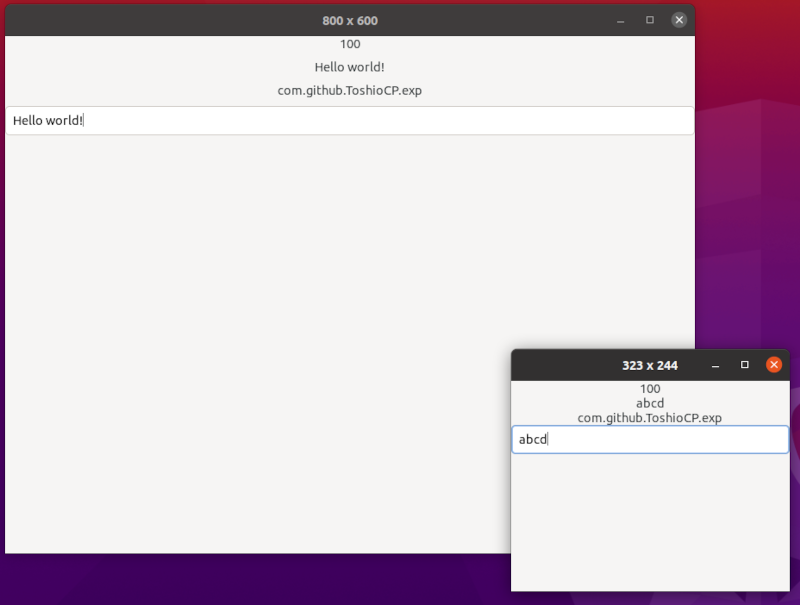
\includegraphics[width=12cm,height=9.1cm]{../image/expression.png}
\caption{Expression}
\end{figure}

If you put some text in the field of the entry, then the same text
appears in the second GtkLabel. Because the ``label'' property of the
second GtkLabel instance is bound to the text in the GtkEntryBuffer.

If you resize the window, then the size appears in the title bar because
the ``title'' property is bound to ``default-width'' and
``default-height'' properties.

  \hypertarget{gtkcolumnview}{%
\section{GtkColumnView}\label{gtkcolumnview}}

\hypertarget{gtkcolumnview-1}{%
\subsection{GtkColumnView}\label{gtkcolumnview-1}}

GtkColumnView is like GtkListView, but it has multiple columns. Each
column is GtkColumnViewColumn.

\begin{figure}
\centering
\includegraphics[width=11.3cm,height=9cm]{../image/column_view.png}
\caption{Column View}
\end{figure}

\begin{itemize}
\tightlist
\item
  GtkColumnView has ``model'' property. The property points a
  GtkSelectionModel object.
\item
  Each GtkColumnViewColumn has ``factory'' property. The property points
  a GtkListItemFactory (GtkSignalListItemFactory or
  GtkBuilderListItemFactory).
\item
  The factory connects GtkListItem, which belongs to
  GtkColumnViewColumn, and items of GtkSelectionModel. And the factory
  builds the descendants widgets of GtkColumnView to display the item on
  the display. This process is the same as the one in GtkListView.
\end{itemize}

The following diagram shows the image how it works.

\begin{figure}
\centering
\includegraphics[width=12cm,height=9cm]{../image/column.png}
\caption{ColumnView}
\end{figure}

The example in this section is a window that displays information of
files in a current directory. The information is the name, size and last
modified datetime of files. So, there are three columns.

In addition, the example uses GtkSortListModel and GtkSorter to sort the
information.

\hypertarget{column.ui}{%
\subsection{column.ui}\label{column.ui}}

Ui file specifies whole widgets and their structure.

\begin{lstlisting}[language=XML, numbers=left]
<?xml version="1.0" encoding="UTF-8"?>
<interface>
  <object class="GtkApplicationWindow" id="win">
    <property name="title">file list</property>
    <property name="default-width">800</property>
    <property name="default-height">600</property>
    <child>
      <object class="GtkScrolledWindow" id="scr">
        <property name="hexpand">TRUE</property>
        <property name="vexpand">TRUE</property>
        <child>
          <object class="GtkColumnView" id="columnview">
            <property name="model">
              <object class="GtkSingleSelection" id="singleselection">
                <property name="model">
                  <object class="GtkSortListModel" id="sortlist">
                    <property name="model">
                      <object class="GtkDirectoryList" id="directorylist">
                        <property name="attributes">standard::name,standard::icon,standard::size,time::modified</property>
                      </object>
                    </property>
                    <binding name="sorter">
                      <lookup name="sorter">columnview</lookup>
                    </binding>
                  </object>
                </property>
              </object>
            </property>
            <child>
              <object class="GtkColumnViewColumn" id="column1">
                <property name="title">Name</property>
                <property name="expand">TRUE</property>
                <property name="factory">
                  <object class="GtkBuilderListItemFactory">
                    <property name="bytes"><![CDATA[
<?xml version="1.0" encoding="UTF-8"?>
<interface>
  <template class="GtkListItem">
    <property name="child">
      <object class="GtkBox">
        <property name="orientation">GTK_ORIENTATION_HORIZONTAL</property>
        <property name="spacing">20</property>
        <child>
          <object class="GtkImage">
            <binding name="gicon">
              <closure type="GIcon" function="get_icon_factory">
                <lookup name="item">GtkListItem</lookup>
              </closure>
            </binding>
          </object>
        </child>
        <child>
          <object class="GtkLabel">
            <property name="hexpand">TRUE</property>
            <property name="xalign">0</property>
            <binding name="label">
              <closure type="gchararray" function="get_file_name_factory">
                <lookup name="item">GtkListItem</lookup>
              </closure>
            </binding>
          </object>
        </child>
      </object>
    </property>
  </template>
</interface>
                    ]]></property>
                  </object>
                </property>
                <property name="sorter">
                  <object class="GtkStringSorter" id="sorter_name">
                    <property name="expression">
                      <closure type="gchararray" function="get_file_name">
                      </closure>
                    </property>
                  </object>
                </property>
              </object>
            </child>
            <child>
              <object class="GtkColumnViewColumn" id="column2">
                <property name="title">Size</property>
                <property name="factory">
                  <object class="GtkBuilderListItemFactory">
                    <property name="bytes"><![CDATA[
<?xml version="1.0" encoding="UTF-8"?>
<interface>
  <template class="GtkListItem">
    <property name="child">
      <object class="GtkLabel">
        <property name="hexpand">TRUE</property>
        <property name="xalign">0</property>
        <binding name="label">
          <closure type="gchararray" function="get_file_size_factory">
            <lookup name="item">GtkListItem</lookup>
          </closure>
        </binding>
      </object>
    </property>
  </template>
</interface>
                    ]]></property>
                  </object>
                </property>
                <property name="sorter">
                  <object class="GtkNumericSorter" id="sorter_size">
                    <property name="expression">
                      <closure type="gint64" function="get_file_size">
                      </closure>
                    </property>
                    <property name="sort-order">GTK_SORT_ASCENDING</property>
                  </object>
                </property>
              </object>
            </child>
            <child>
              <object class="GtkColumnViewColumn" id="column3">
                <property name="title">Date modified</property>
                <property name="factory">
                  <object class="GtkBuilderListItemFactory">
                    <property name="bytes"><![CDATA[
<?xml version="1.0" encoding="UTF-8"?>
<interface>
  <template class="GtkListItem">
    <property name="child">
      <object class="GtkLabel">
        <property name="hexpand">TRUE</property>
        <property name="xalign">0</property>
        <binding name="label">
          <closure type="gchararray" function="get_file_time_modified_factory">
            <lookup name="item">GtkListItem</lookup>
          </closure>
        </binding>
      </object>
    </property>
  </template>
</interface>
                    ]]></property>
                  </object>
                </property>
                <property name="sorter">
                  <object class="GtkNumericSorter" id="sorter_datetime_modified">
                    <property name="expression">
                      <closure type="gint64" function="get_file_unixtime_modified">
                      </closure>
                    </property>
                    <property name="sort-order">GTK_SORT_ASCENDING</property>
                  </object>
                </property>
              </object>
            </child>
          </object>
        </child>
      </object>
    </child>
  </object>
</interface>
\end{lstlisting}

\begin{itemize}
\tightlist
\item
  3-12: Widget parent-child relationship is GtkApplicationWindow
  =\textgreater{} GtkScrolledWindow =\textgreater{} GtkColumnView.
\item
  12-18: GtkColumnView has ``model'' property. It points
  GtkSelectionModel interface. In this ui file, GtkSingleSelection is
  used as GtkSelectionModel. GtkSingleSelection is an object that
  implements GtkSelectionModel. And again, it has ``model'' property. It
  points GtkSortListModel. This list model supports sorting the list. It
  will be explained in the later subsection. And it also has ``model''
  property. It points GtkDirectoryList. Therefore, the chain is:
  GtkColumnView =\textgreater{} GtkSingleSelection =\textgreater{}
  GtkSortListModel =\textgreater{} GtkDirectoryList.
\item
  18-20: GtkDirectoryList. It is a list of GFileInfo, which holds
  information of files under a directory. It has ``attributes''
  property. It specifies what attributes is kept in each GFileInfo.

  \begin{itemize}
  \tightlist
  \item
    ``standard::name'' is a name of the file.
  \item
    ``standard::icon'' is a GIcon object of the file
  \item
    ``standard::size'' is the file size.
  \item
    ``time::modified'' is the date and time the file was last modified.
  \end{itemize}
\item
  29-79: The first GtkColumnViewColumn object. There are four
  properties, ``title'', ``expand'', factory" and ``sorter''.
\item
  31: Sets the ``title'' property with ``Name''. This is the title on
  the header of the column.
\item
  32: Sets the ``expand'' property to TRUE to allow the column to expand
  as much as possible. (See the image above).
\item
  33- 69: Sets the ``factory'' property with GtkBuilderListItemFactory.
  The factory has ``bytes'' property which holds a ui string to define a
  template to build GtkListItem composite widget. The CDATA section
  (line 36-66) is the ui string to put into the ``bytes'' property. The
  contents are the same as the ui file
  \passthrough{\lstinline!factory\_list.ui!} in the section 27.
\item
  70-77: Sets the ``sorter'' property with GtkStringSorter object. This
  object provides a sorter that compares strings. It has ``expression''
  property which is set with GtkExpression. A closure tag with a string
  type function \passthrough{\lstinline!get\_file\_name!} is used here.
  The function will be explained later.
\item
  80-115: The second GtkColumnViewColumn object. Its ``title'',
  ``factory'' and ``sorter'' properties are set. GtkNumericSorter is
  used.
\item
  116-151: The third GtkColumnViewColumn object. Its ``title'',
  ``factory'' and ``sorter'' properties are set. GtkNumericSorter is
  used.
\end{itemize}

\hypertarget{gtksortlistmodel-and-gtksorter}{%
\subsection{GtkSortListModel and
GtkSorter}\label{gtksortlistmodel-and-gtksorter}}

GtkSortListModel is a list model that sorts its elements according to a
GtkSorter. It has ``sorter'' property that is set with GtkSorter. The
property is bound to ``sorter'' property of GtkColumnView in line 22 to
24.

\begin{lstlisting}[language=XML]
<object class="GtkSortListModel" id="sortlist">
... ... ...
  <binding name="sorter">
    <lookup name="sorter">columnview</lookup>
  </binding>
\end{lstlisting}

Therefore, \passthrough{\lstinline!columnview!} determines the way how
to sort the list model. The ``sorter'' property of GtkColumnView is
read-only property and it is a special sorter. It reflects the user's
sorting choice. If a user clicks the header of a column, then the sorter
(``sorter'' property) of the column is referenced by ``sorter'' property
of the GtkColumnView. If the user clicks the header of another column,
then the ``sorter'' property of the GtkColumnView refers to the newly
clicked column's ``sorter'' property.

The binding above makes a indirect connection between the ``sorter''
property of GtkSortListModel and the ``sorter'' property of each column.

GtkSorter has several child objects.

\begin{itemize}
\tightlist
\item
  GtkStringSorter compares strings.
\item
  GtkNumericSorter compares numbers.
\item
  GtkCustomSorter uses a callback to compare.
\item
  GtkMultiSorter combines multiple sorters.
\end{itemize}

The example uses GtkStringSorter and GtkNumericSorter.

GtkStringSorter uses GtkExpression to get the strings from the objects.
The GtkExpression is stored in the ``expression'' property of
GtkStringSorter. For example, in the ui file above, the GtkExpression is
in the line 71 to 76.

\begin{lstlisting}[language=XML]
<object class="GtkStringSorter" id="sorter_name">
  <property name="expression">
    <closure type="gchararray" function="get_file_name">
    </closure>
  </property>
</object>
\end{lstlisting}

The GtkExpression calls \passthrough{\lstinline!get\_file\_name!}
function when it is evaluated.

\begin{lstlisting}[language=C, numbers=left]
char *
get_file_name (GFileInfo *info) {
  g_return_val_if_fail (G_IS_FILE_INFO (info), NULL);

  return g_strdup(g_file_info_get_name (info));
}
\end{lstlisting}

The function is given the item (GFileInfo) of the GtkSortListModel as an
argument (\passthrough{\lstinline!this!} object). The function retrieves
a filename from \passthrough{\lstinline!info!}. The string is owned by
\passthrough{\lstinline!info!} so it is necessary to duplicate it. And
it returns the copied string. The string will be owned by the
expression.

GtkNumericSorter compares numbers. It is used in the line 106 to 112 and
line 142 to 148. The lines from 106 to 112 is:

\begin{lstlisting}[language=XML]
<object class="GtkNumericSorter" id="sorter_size">
  <property name="expression">
    <closure type="gint64" function="get_file_size">
    </closure>
  </property>
  <property name="sort-order">GTK_SORT_ASCENDING</property>
</object>
\end{lstlisting}

The closure tag specifies a callback function
\passthrough{\lstinline!get\_file\_size!}.

\begin{lstlisting}[language=C, numbers=left]
goffset
get_file_size (GFileInfo *info) {
  g_return_val_if_fail (G_IS_FILE_INFO (info), -1);

  return g_file_info_get_size (info);
}
\end{lstlisting}

It just returns the size of \passthrough{\lstinline!info!}. The type of
the size is \passthrough{\lstinline!goffset!}. The type
\passthrough{\lstinline!goffset!} is the same as
\passthrough{\lstinline!gint64!}.

The lines from 142 to 148 is:

\begin{lstlisting}[language=XML]
<object class="GtkNumericSorter" id="sorter_datetime_modified">
  <property name="expression">
    <closure type="gint64" function="get_file_unixtime_modified">
    </closure>
  </property>
  <property name="sort-order">GTK_SORT_ASCENDING</property>
</object>
\end{lstlisting}

The closure tag specifies a callback function
\passthrough{\lstinline!get\_file\_unixtime\_modified!}.

\begin{lstlisting}[language=C, numbers=left]
gint64
get_file_unixtime_modified (GFileInfo *info) {
  g_return_val_if_fail (G_IS_FILE_INFO (info), -1);

  GDateTime *dt;

  dt = g_file_info_get_modification_date_time (info);
  return g_date_time_to_unix (dt);
}
\end{lstlisting}

It gets the modification date and time (GDateTime type) of
\passthrough{\lstinline!info!}. Then it gets a unix time from
\passthrough{\lstinline!dt!}. Unix time, sometimes called unix epoch, is
the number of seconds that have elapsed since 00:00:00 UTC on 1 January
1970. It returns the unix time (gint64 type).

\hypertarget{column.c}{%
\subsection{column.c}\label{column.c}}

\passthrough{\lstinline!column.c!} is as follows.

\begin{lstlisting}[language=C, numbers=left]
#include <gtk/gtk.h>

/* functions (closures) for GtkBuilderListItemFactory */
GIcon *
get_icon_factory (GtkListItem *item, GFileInfo *info) {
  GIcon *icon;
  if (! G_IS_FILE_INFO (info))
    return NULL;
  else {
    icon = g_file_info_get_icon (info);
    g_object_ref (icon);
    return icon;
  }
}

char *
get_file_name_factory (GtkListItem *item, GFileInfo *info) {
  if (! G_IS_FILE_INFO (info))
    return NULL;
  else
    return g_strdup (g_file_info_get_name (info));
}

char *
get_file_size_factory (GtkListItem *item, GFileInfo *info) {
  /* goffset is gint64 */
  goffset size;

  if (! G_IS_FILE_INFO (info))
    return NULL;
  else {
    size = g_file_info_get_size (info);
    return g_strdup_printf ("%ld", (long int) size);
  }
}

char *
get_file_time_modified_factory (GtkListItem *item, GFileInfo *info) {
  GDateTime *dt;

  if (! G_IS_FILE_INFO (info))
    return NULL;
  else {
    dt = g_file_info_get_modification_date_time (info);
    return g_date_time_format (dt, "%F");
  }
}

/* Functions (closures) for GtkSorter */
char *
get_file_name (GFileInfo *info) {
  g_return_val_if_fail (G_IS_FILE_INFO (info), NULL);

  return g_strdup(g_file_info_get_name (info));
}

goffset
get_file_size (GFileInfo *info) {
  g_return_val_if_fail (G_IS_FILE_INFO (info), -1);

  return g_file_info_get_size (info);
}

gint64
get_file_unixtime_modified (GFileInfo *info) {
  g_return_val_if_fail (G_IS_FILE_INFO (info), -1);

  GDateTime *dt;

  dt = g_file_info_get_modification_date_time (info);
  return g_date_time_to_unix (dt);
}

/* ----- activate, open, startup handlers ----- */
static void
app_activate (GApplication *application) {
  GtkApplication *app = GTK_APPLICATION (application);
  GFile *file;

  GtkBuilder *build = gtk_builder_new_from_resource ("/com/github/ToshioCP/column/column.ui");
  GtkWidget *win = GTK_WIDGET (gtk_builder_get_object (build, "win"));
  GtkDirectoryList *directorylist = GTK_DIRECTORY_LIST (gtk_builder_get_object (build, "directorylist"));
  g_object_unref (build);

  gtk_window_set_application (GTK_WINDOW (win), app);

  file = g_file_new_for_path (".");
  gtk_directory_list_set_file (directorylist, file);
  g_object_unref (file);

  gtk_widget_show (win);
}

static void
app_startup (GApplication *application) {
}

#define APPLICATION_ID "com.github.ToshioCP.columnview"

int
main (int argc, char **argv) {
  GtkApplication *app;
  int stat;

  app = gtk_application_new (APPLICATION_ID, G_APPLICATION_FLAGS_NONE);

  g_signal_connect (app, "startup", G_CALLBACK (app_startup), NULL);
  g_signal_connect (app, "activate", G_CALLBACK (app_activate), NULL);
/*  g_signal_connect (app, "open", G_CALLBACK (app_open), NULL);*/

  stat =g_application_run (G_APPLICATION (app), argc, argv);
  g_object_unref (app);
  return stat;
}
\end{lstlisting}

\begin{itemize}
\tightlist
\item
  4-47: Functions for the closure tag in the ``bytes'' property of
  GtkBuilderListItemFactory. These are almost same as the functions in
  section 26 and 26.
\item
  50-72: Functions for the closure in the expression property of
  GtkStringSorter or GtkNumericSorter.
\item
  75-92: \passthrough{\lstinline!app\_activate!} is an ``activate''
  handler of GApplication.
\item
  80-83: Builds objects with ui resource and gets
  \passthrough{\lstinline!win!} and
  \passthrough{\lstinline!directorylist!}.
\item
  85: Sets the application of the top level window with
  \passthrough{\lstinline!app!}.
\item
  87-89: Sets the file of \passthrough{\lstinline!directorylist!} with
  ``.'' (current directory).
\item
  94-96: Startup handler.
\item
  98-114: \passthrough{\lstinline!main!} function.
\end{itemize}

\passthrough{\lstinline!exp.c!} is simple and short thanks to
\passthrough{\lstinline!exp.ui!}.

\hypertarget{compilation-and-execution.}{%
\subsection{Compilation and
execution.}\label{compilation-and-execution.}}

All the source files are in src/column directory. Change your current
directory to the directory and type the following.

\begin{lstlisting}
$ meson _build
$ ninja -C _build
$ _build/column
\end{lstlisting}

Then, a window appears.

\begin{figure}
\centering
\includegraphics[width=11.3cm,height=9cm]{../image/column_view.png}
\caption{Column View}
\end{figure}

If you click the header of a column, then the whole lists are sorted by
the column. If you click the header of another column, then the whole
lists are sorted by the newly selected column.

GtkColumnView is very useful and it can manage very big GListModel. It
is possible to use it for file list, application list, database frontend
and so on.

\newpage
\appendix
  \hypertarget{turtles-manual}{%
\section{Turtle's manual}\label{turtles-manual}}

Turtle is a simple interpreter for turtle graphics.

\hypertarget{prerequisite-and-compiling}{%
\subsection{Prerequisite and
compiling}\label{prerequisite-and-compiling}}

Turtle is written in C language. You need:

\begin{itemize}
\tightlist
\item
  Linux. Turtle is tested on ubuntu 20.10
\item
  gcc, meson and ninja
\item
  gtk4
\end{itemize}

It is easy to compile the source file of turtle. If you have installed
gtk4 with an option \passthrough{\lstinline!--prefix=$HOME/local!}, put
the same option to meson so that you can install
\passthrough{\lstinline!turtle!} under the directory
\passthrough{\lstinline!$HOME/local/bin!}. The instruction is:

\begin{lstlisting}
$ meson --prefix=$HOME/local _build
$ ninja -C _build
$ ninja -C _build install
\end{lstlisting}

Type the following command then turtle shows the following window.

\begin{lstlisting}
$ turtle
\end{lstlisting}

\begin{figure}
\centering
\includegraphics[width=8cm,height=5.11cm]{../src/turtle/image/turtle1.png}
\caption{Screenshot just after it's executed}
\end{figure}

The left half is a text editor and the right half is a surface. Surface
is like a canvas to draw shapes.

Write turtle language in the text editor and click on
\passthrough{\lstinline!run!} button, then the program will be executed
and it draws shapes on the surface.

\begin{figure}
\centering
\includegraphics[width=8cm,height=5.11cm]{../src/turtle/image/turtle_tree.png}
\caption{Tree}
\end{figure}

If you add the following line in \passthrough{\lstinline!turtle.h!},
then codes to inform the status will also be compiled. However, the
speed will be quite slow because of the output messages.

\begin{lstlisting}
# define debug 1
\end{lstlisting}

\hypertarget{example}{%
\subsection{Example}\label{example}}

Imagine a turtle. The turtle has a pen and initially he is at the center
of the screen, facing to the north (to the north means up on the
screen). You can let the turtle down the pen or up the pen. You can
order the turtle to move forward.

\begin{lstlisting}
pd
fd 100
\end{lstlisting}

\begin{itemize}
\tightlist
\item
  pd: Pen Down. The turtle put the pen down so that the turtle will draw
  a line if he/she moves.
\item
  fd 100: move ForwarD 100. The turtle goes forward 100 pixels.
\end{itemize}

If you click on \passthrough{\lstinline!run!} button, then a line
segment appears on the screen. One of the endpoints of the line segment
is at the center of the surface and the other is at 100 pixels up from
the center. The point at the center is the start point of the turtle and
the other endpoint is the end point of the movement.

If the turtle picks the pen up, then no line segment appears.

\begin{lstlisting}
pu
fd 100
\end{lstlisting}

The command \passthrough{\lstinline!pu!} means ``Pen Up''.

The turtle can change the direction.

\begin{lstlisting}
pd
fd 100
tr 90
fd 100
\end{lstlisting}

The command \passthrough{\lstinline!tr!} is ``Turn Right''. The argument
is angle with degrees. Therefore, \passthrough{\lstinline!tr 90!} means
``Turn right by 90 degrees''. If you click on the
\passthrough{\lstinline!run!}button, then two line segments appears. One
is vertical and the other is horizontal.

\begin{figure}
\centering
\includegraphics[width=8cm,height=5.11cm]{../src/turtle/image/turtle2.png}
\caption{Two line segments on the surface}
\end{figure}

\hypertarget{background-and-foreground-color}{%
\subsection{Background and foreground
color}\label{background-and-foreground-color}}

Colors are specified with RGB. A vector (r, g, b) denotes RGB color.
Each of the elements is a real number between 0 and 1.

\begin{itemize}
\tightlist
\item
  Red is (1.0, 0.0, 0.0). You can write (1, 0, 0) instead.
\item
  Green is (0.0, 1.0, 0.0)
\item
  Blue is (0.0, 0.0, 1.0)
\item
  Black is (0.0, 0.0, 0.0)
\item
  White is (1.0, 1.0, 1.0)
\end{itemize}

You can express a variety of colors by changing each element.

There are two commands to change colors.

\begin{itemize}
\tightlist
\item
  bc: Background Color. \passthrough{\lstinline!bc (1,0,0)!} changes the
  background color to red. This command clear the surface and change the
  background color. So, the shapes on the surface disappears.
\item
  fc: Foreground Color. \passthrough{\lstinline!fc (0,1,0)!} changes the
  foreground color to green. This command changes the pen color. The
  prior shapes on the surface aren't affected. After this command, the
  turtle draws lines with the new color.
\end{itemize}

\begin{figure}
\centering
\includegraphics[width=8cm,height=5.11cm]{../src/turtle/image/turtle3.png}
\caption{Change the foreground color}
\end{figure}

\hypertarget{other-simple-commands}{%
\subsection{Other simple commands}\label{other-simple-commands}}

\begin{itemize}
\tightlist
\item
  pw: Pen Width. This is the same as pen size or line width. For
  example, \passthrough{\lstinline!pw 5!} makes lines thick and
  \passthrough{\lstinline!pw 1!} makes it thin.
\item
  rs: ReSet. The turtle moves back to the initial position and
  direction. In addition, The command initialize the pen, line width
  (pen size), and foreground color. The pen is down, the line width is 2
  and the foreground color is black.
\end{itemize}

An order such as \passthrough{\lstinline!fd 100!},
\passthrough{\lstinline!pd!} and so on is a statement. Statements are
executed in the order from the top to the end

\hypertarget{comment-and-spaces}{%
\subsection{Comment and spaces}\label{comment-and-spaces}}

Characters between \passthrough{\lstinline!\#!} (hash mark) and
\passthrough{\lstinline!\\n!} (new line) inclusive are comment. If the
comment is at the end of the file, the trailing new line can be left
out. Comments are ignored.

\begin{lstlisting}
# draw a triangle
fd 100 # forward 100 pixels<NEW LINE>
tr 120 # turn right by 90 degrees<NEW LINE>
fd 100<NEW LINE>
tr 120<NEW LINE>
fd 100 # Now a triangle appears.<EOF>
\end{lstlisting}

\textless NEW LINE\textgreater{} and \textless EOF\textgreater{}
indicate newline code and end of file respectively. The comments in the
line 1, 2, 3 and 6 are correct syntactically.

Spaces (white space, tab and new line) are ignored. They are used only
as delimiters. Tabs are recognized as eight spaces to calculate the
column number.

\hypertarget{variables-and-expressions}{%
\subsection{Variables and expressions}\label{variables-and-expressions}}

Variable begins alphabet followed by alphabet or digit. Key words like
\passthrough{\lstinline!fd!}, \passthrough{\lstinline!tr!} can't be
variables. \passthrough{\lstinline!Distance!} and
\passthrough{\lstinline!angle5!} are variables, but
\passthrough{\lstinline!1step!} isn't a variable because the first
character isn't alphabet. Variable names are case sensitive. Variables
keep real numbers. Their type is the same as
\passthrough{\lstinline!double!} in C language. Integers are casted to
real numbers automatically. So 1 and 1.0 are the same value. Numbers
begin digits, not signs (\passthrough{\lstinline!+!} or
\passthrough{\lstinline!-!}).

\begin{itemize}
\tightlist
\item
  100, 20.34 and 0.01 are numbers
\item
  +100 isn't a number. It causes syntax error. Use 100 instead.
\item
  -100 isn't a number. But turtle recognizes it unary minus and a number
  100. So turtle calculate it and the result is -100.
\item
  100 + -20: This is recognized 100 + (- 20). However, using bracket,
  100 + (-20), is better for easy reading.
\end{itemize}

\begin{lstlisting}
distance = 100
fd distance
\end{lstlisting}

A value 100 is assigned to the variable
\passthrough{\lstinline!distance!} in the first line. Assignment is a
statement. Most of statements begin with commands like
\passthrough{\lstinline!fd!}. Assignment is the only exception.

The example above draws a line segment of 100 pixels long.

You can use variables in expressions. There are 8 kinds of calculations
available.

\begin{itemize}
\tightlist
\item
  addition: x + y
\item
  subtraction: x - y
\item
  multiplication: x * y
\item
  division: x / y
\item
  unary minus: - x
\item
  logical equal: x = y. This symbol \passthrough{\lstinline!=!} works as
  \passthrough{\lstinline!==!} in C language.
\item
  greater than: x \textgreater{} y
\item
  less than: x \textless{} y
\end{itemize}

The last three symbols are mainly used in the condition of if statement.

Variables are registered to a symbol table when it is assigned a value
for the first time. Evaluating a variable before the registration isn't
allowed and occurs an error.

\hypertarget{if-statement}{%
\subsection{If statement}\label{if-statement}}

Turtle language has very simple if statement.

\begin{lstlisting}
if (x > 50) {
  fd x
}
\end{lstlisting}

There is no else part.

\hypertarget{procedures}{%
\subsection{Procedures}\label{procedures}}

Procedures are similar to functions in C language. The difference is
that procedures don't have return values.

\begin{lstlisting}
dp triangle (side) {
  fd side
  tr 120
  fd side
  tr 120
  fd side
}

triangle (100)
\end{lstlisting}

\passthrough{\lstinline!dp!} (Define Procedure) is a key word followed
by procedure name, parameters, and body. Procedure names start alphabet
followed by alphabet or digit. Parameters are a list of variables. For
example

\begin{lstlisting}
dp abc (a) { ... ... }
dp abc (a, b) { ... ... }
dp abc (a, b, c) { ... ... }
\end{lstlisting}

Body is a sequence of statements. The statements aren't executed when
the procedure is defined. They will be executed when the procedure is
called later.

Procedures are called by the name followed by arguments.

\begin{lstlisting}
dp proc (a, b, c) { ... ... }

proc (100, 0, -20*3)
\end{lstlisting}

The number of parameters and arguments must be the same. Arguments can
be any expressions. When you call a procedure, brackets following the
procedure name must exist even if the procedure has no argument.

Procedure names and variable names don't conflict.

\begin{lstlisting}
dp a () {fd a}
a=100
a ()
\end{lstlisting}

This is a correct program.

\begin{itemize}
\tightlist
\item
  1: Defines a procedure \passthrough{\lstinline!a!}. A variable
  \passthrough{\lstinline!a!} is in its body.
\item
  2: Assigns 100 to a variable \passthrough{\lstinline!a!}.
\item
  3: Procedure \passthrough{\lstinline!a!} is called.
\end{itemize}

However, using the same name to a procedure and variable makes
confusing. You should avoid that.

\hypertarget{recursive-call}{%
\subsection{Recursive call}\label{recursive-call}}

Procedures can be called recursively.

\begin{lstlisting}
dp repeat (n) {
  n = n - 1
  if (n < 0) {
    rt
  }
  fd 100
  tr 90
  repeat (n)
}

repeat (4)
\end{lstlisting}

Repeat is called in the body of repeat. The call to itself is a
recursive call. Parameters are created and set each time the procedure
is called. So, parameter \passthrough{\lstinline!n!} is 4 at the first
call but it is 3 at the second call. Each time the procedure is called,
the parameter \passthrough{\lstinline!n!} decreases by one. Finally, it
becomes less than zero, then the procedures return.

The program above draws a square.

Turtle doesn't have any primary loop statements. It should probably be
added to the future version. However, the program above shows that we
can program loop with a recursive call.

\hypertarget{fractal-curves}{%
\subsection{Fractal curves}\label{fractal-curves}}

Recursive call can be applied to draw fractal curves. Fractal curves
appear when a procedure is applied to it repeatedly. The procedure
replaces a part of the curve with the contracted curve.

\begin{figure}
\centering
\includegraphics[width=8cm,height=5.11cm]{../src/turtle/image/turtle_tree.png}
\caption{Tree}
\end{figure}

This shape is called tree. The basic pattern of this shape is a line
segment. It is the first stage. The second stage adds two shorter line
segments at the endpoint of the original segment. The new segment has 70
percent length to the original segment and the orientation is +30 or -30
degrees different. The third stage adds two shorter line segments to the
second stage line segments. And repeats it several times.

This repeating is programmed by recursive call. Two more examples are
shown here. They are Koch curve and Square Koch curve.

\begin{figure}
\centering
\includegraphics[width=8cm,height=5.11cm]{../src/turtle/image/turtle_koch.png}
\caption{Koch curve}
\end{figure}

\begin{figure}
\centering
\includegraphics[width=8cm,height=5.11cm]{../src/turtle/image/turtle_square_koch.png}
\caption{Square Koch curve}
\end{figure}

\hypertarget{tokens-and-punctuations}{%
\subsection{Tokens and punctuations}\label{tokens-and-punctuations}}

The following is the list of tokens.

Keywords:

\begin{itemize}
\tightlist
\item
  pu: pen up
\item
  pd: pen down
\item
  pw: pen width = line width
\item
  fd: forward
\item
  tr: turn right
\item
  bc: background color
\item
  fc: foreground color
\item
  if: if statement
\item
  rt: return
\item
  rs: reset
\item
  dp: define procedure
\end{itemize}

identifiers and numbers:

\begin{itemize}
\tightlist
\item
  identifier: This is used for the name of variables, parameters and
  procedures. It is expressed
  \passthrough{\lstinline![a-zA-Z][a-zA-Z0-9]*!} in regular expression.
\item
  number: This is expressed
  \passthrough{\lstinline!(0|[1-9][0-9]*)(\\.[0-9]+)?!} in regular
  expression. It doesn't have \passthrough{\lstinline!+!} or
  \passthrough{\lstinline!-!} sign because they bring some syntactic
  confusion. However negative number such as
  \passthrough{\lstinline!-10!} can be recognized as unary minus and a
  number.
\end{itemize}

Symbols for expression

\begin{itemize}
\tightlist
\item
  \passthrough{\lstinline!=!}
\item
  \passthrough{\lstinline!>!}
\item
  \passthrough{\lstinline!<!}
\item
  \passthrough{\lstinline!+!}
\item
  \passthrough{\lstinline!-!}
\item
  \passthrough{\lstinline!*!}
\item
  \passthrough{\lstinline!/!}
\item
  \passthrough{\lstinline!(!}
\item
  \passthrough{\lstinline!)!}
\end{itemize}

Delimiters

\begin{itemize}
\tightlist
\item
  \passthrough{\lstinline!(!}
\item
  \passthrough{\lstinline!)!}
\item
  \passthrough{\lstinline!\{!}
\item
  \passthrough{\lstinline!\}!}
\item
  \passthrough{\lstinline!,!}
\end{itemize}

Comments and spaces:

\begin{itemize}
\tightlist
\item
  comment: This is characters between \passthrough{\lstinline!\#!} and
  new line inclusive. If a comment is at the end of the file, the
  trailing new line can be left out.
\item
  white space:
\item
  horizontal tab: tab is recognized as eight spaces.
\item
  new line: This is the end of a line.
\end{itemize}

These characters are used to separate tokens explicitly. They doesn't
have any syntactic meaning and are ignored by the parser.

\hypertarget{grammar}{%
\subsection{Grammar}\label{grammar}}

\begin{lstlisting}
program:
  statement
| program statement
;

statement:
  primary_procedure
| procedure_definition
;

primary_procedure:
  PU
| PD
| PW expression
| FD expression
| TR expression
| BC '(' expression ',' expression ',' expression ')'
| FC '(' expression ',' expression ',' expression ')'
| ID '=' expression
| IF '(' expression ')' '{' primary_procedure_list '}'
| RT
| RS
| ID '(' ')'
| ID '(' argument_list ')'
;

procedure_definition:
  DP ID '('  ')' '{' primary_procedure_list '}'
| DP ID '(' parameter_list ')' '{' primary_procedure_list '}'
;

parameter_list:
  ID
| parameter_list ',' ID
;

argument_list:
  expression
| argument_list ',' expression
;

primary_procedure_list:
  primary_procedure
| primary_procedure_list primary_procedure
;

expression:
  expression '=' expression
| expression '>' expression
| expression '<' expression
| expression '+' expression
| expression '-' expression
| expression '*' expression
| expression '/' expression
| '-' expression %prec UMINUS
| '(' expression ')'
| ID
| NUM
;
\end{lstlisting}

  \hypertarget{tfetextview-api-reference}{%
\section{TfeTextView API reference}\label{tfetextview-api-reference}}

TfeTextView -- Child object of GtkTextView. It holds GFile which the
contents of GtkTextBuffer correponds to.

\hypertarget{functions}{%
\subsection{Functions}\label{functions}}

\begin{itemize}
\tightlist
\item
  GFile *tfe\_text\_view\_get\_file ()
\item
  void tfe\_text\_view\_open ()
\item
  void tfe\_text\_view\_save ()
\item
  void tfe\_text\_view\_saveas ()
\item
  GtkWidget *tfe\_text\_view\_new\_with\_file ()
\item
  GtkWidget *tfe\_text\_view\_new ()
\end{itemize}

\hypertarget{signals}{%
\subsection{Signals}\label{signals}}

\begin{itemize}
\tightlist
\item
  void change-file
\item
  void open-response
\end{itemize}

\hypertarget{types-and-values}{%
\subsection{Types and Values}\label{types-and-values}}

\begin{itemize}
\tightlist
\item
  TfeTextView
\item
  TfeTextViewClass
\item
  TfeTextViewOpenResponseType
\end{itemize}

\hypertarget{object-hierarchy}{%
\subsection{Object Hierarchy}\label{object-hierarchy}}

\begin{lstlisting}
GObject
+--GInitiallyUnowned
   +--GtkWidget
      +--GtkTextView
         +--TfeTextView
\end{lstlisting}

\hypertarget{includes}{%
\subsection{Includes}\label{includes}}

\begin{lstlisting}
#include <gtk/gtk.h>
\end{lstlisting}

\hypertarget{description}{%
\subsection{Description}\label{description}}

TfeTextView holds GFile which the contents of GtkTextBuffer corresponds
to. File manipulation functions are added to this object.

\hypertarget{functions-1}{%
\subsection{Functions}\label{functions-1}}

\hypertarget{tfe_text_view_get_file}{%
\subsubsection{tfe\_text\_view\_get\_file()}\label{tfe_text_view_get_file}}

\begin{lstlisting}
GFile *
tfe_text_view_get_file (TfeTextView *tv);
\end{lstlisting}

Returns the copy of the GFile in the TfeTextView.

Parameters

\begin{itemize}
\tightlist
\item
  tv: a TfeTextView
\end{itemize}

\hypertarget{tfe_text_view_open}{%
\subsubsection{tfe\_text\_view\_open()}\label{tfe_text_view_open}}

\begin{lstlisting}
void
tfe_text_view_open (TfeTextView *tv, GtkWidget *win);
\end{lstlisting}

Just shows a GtkFileChooserDialog so that a user can choose a file to
read. This function doesn't do any I/O operations. They are done by the
signal handler connected to the \passthrough{\lstinline!response!}
signal emitted by GtkFileChooserDialog. Therefore the caller can't know
the I/O status directly from the function. Instead, the status is
informed by \passthrough{\lstinline!open-response!} signal. The caller
needs to set a handler to this signal in advance.

parameters

\begin{itemize}
\tightlist
\item
  tv: a TfeTextView
\item
  win: the top level window
\end{itemize}

\hypertarget{tfe_text_view_save}{%
\subsubsection{tfe\_text\_view\_save()}\label{tfe_text_view_save}}

\begin{lstlisting}
void
tfe_text_view_save (TfeTextView *tv);
\end{lstlisting}

Saves the contents of a TfeTextView to a file. If
\passthrough{\lstinline!tv!} holds a GFile, it is used. Otherwise, this
function shows GtkFileChosserDialog so that a user can choose a file to
save.

Parameters

\begin{itemize}
\tightlist
\item
  tv: a TfeTextView
\end{itemize}

\hypertarget{tfe_text_view_saveas}{%
\subsubsection{tfe\_text\_view\_saveas()}\label{tfe_text_view_saveas}}

\begin{lstlisting}
void
tfe_text_view_saveas (TfeTextView *tv);
\end{lstlisting}

Saves the content of a TfeTextView to a file. This function shows
GtkFileChosserDialog so that a user can choose a file to save.

Parameters

\begin{itemize}
\tightlist
\item
  tv: a TfeTextView
\end{itemize}

\hypertarget{tfe_text_view_new_with_file}{%
\subsubsection{tfe\_text\_view\_new\_with\_file()}\label{tfe_text_view_new_with_file}}

\begin{lstlisting}
GtkWidget *
tfe_text_view_new_with_file (GFile *file);
\end{lstlisting}

Creates a new TfeTextView and reads the contents of the
\passthrough{\lstinline!file!} and set it to the GtkTextBuffer
corresponds to the newly created TfeTextView. Then returns the
TfeTextView as GtkWidget. If an error happens, it returns
\passthrough{\lstinline!NULL!}.

Parameters

\begin{itemize}
\tightlist
\item
  file: a GFile
\end{itemize}

Returns

\begin{itemize}
\tightlist
\item
  a new TfeTextView.
\end{itemize}

\hypertarget{tfe_text_view_new}{%
\subsubsection{tfe\_text\_view\_new()}\label{tfe_text_view_new}}

\begin{lstlisting}
GtkWidget *
tfe_text_view_new (void);
\end{lstlisting}

Creates a new TfeTextView and returns the TfeTextView as GtkWidget. If
an error happens, it returns \passthrough{\lstinline!NULL!}.

Returns

\begin{itemize}
\tightlist
\item
  a new TfeTextView.
\end{itemize}

\hypertarget{types-and-values-1}{%
\subsection{Types and Values}\label{types-and-values-1}}

\hypertarget{tfetextview}{%
\subsubsection{TfeTextView}\label{tfetextview}}

\begin{lstlisting}
typedef struct _TfeTextView TfeTextView
struct _TfeTextView
{
  GtkTextView parent;
  GFile *file;
};
\end{lstlisting}

The members of this structure are not allowed to be accessed by any
outer objects. If you want to obtain a copy of the GFile, use
\passthrough{\lstinline!tfe\_text\_view\_get\_file!}.

\hypertarget{tfetextviewclass}{%
\subsubsection{TfeTextViewClass}\label{tfetextviewclass}}

\begin{lstlisting}
typedef struct {
  GtkTextViewClass parent_class;
} TfeTextViewClass;
\end{lstlisting}

No member is added because TfeTextView is a final type object.

\hypertarget{enum-tfetextviewopenresponsetype}{%
\subsubsection{enum
TfeTextViewOpenResponseType}\label{enum-tfetextviewopenresponsetype}}

Predefined values for the response id given by
\passthrough{\lstinline!open-response!} signal.

Members:

\begin{itemize}
\tightlist
\item
  TFE\_OPEN\_RESPONSE\_SUCCESS: The file is successfully opened.
\item
  TFE\_OPEN\_RESPONSE\_CANCEL: Reading file is canceled by the user.
\item
  TFE\_OPEN\_RESPONSE\_ERROR: An error happened during the opening or
  reading process.
\end{itemize}

\hypertarget{signals-1}{%
\subsection{Signals}\label{signals-1}}

\hypertarget{change-file}{%
\subsubsection{change-file}\label{change-file}}

\begin{lstlisting}
void
user_function (TfeTextView *tv,
               gpointer user_data)
\end{lstlisting}

Emitted when the GFile in the TfeTextView object is changed. The signal
is emitted when:

\begin{itemize}
\tightlist
\item
  a new file is opened and read
\item
  a user choose a file with GtkFileChooserDialog and save the contents.
\item
  an error occured during I/O operation, and GFile is removed as a
  result.
\end{itemize}

\hypertarget{open-response}{%
\subsubsection{open-response}\label{open-response}}

\begin{lstlisting}
void
user_function (TfeTextView *tv,
               TfeTextViewOpenResponseType response-id,
               gpointer user_data)
\end{lstlisting}

Emitted after the user calls
\passthrough{\lstinline!tfe\_text\_view\_open!}. This signal informs the
status of file opening and reading.

  \hypertarget{construir-el-tutorial-de-gtk4}{%
\section{Construir el Tutorial de
Gtk4}\label{construir-el-tutorial-de-gtk4}}

\hypertarget{guuxeda-ruxe1pida}{%
\subsection{Guía rápida}\label{guuxeda-ruxe1pida}}

\begin{enumerate}
\def\labelenumi{\arabic{enumi}.}
\tightlist
\item
  Necesitas el sistema operativo linux, ruby, make, pandoc y latex
  instalados.
\item
  Descarga este repositorio y descomprime el archivo.
\item
  Cambia al directorio superior de los archivos fuente.
\item
  Escribe \texttt{rake\ html} para crear archivos html. Los archivos se
  crearán dentro de la carpeta \texttt{docs}.
\item
  Escribe \texttt{rake\ pdf}para crear el pdf. El archivo se creará
  dentro de la carpeta \texttt{latex}.
\end{enumerate}

\hypertarget{prerequisitos}{%
\subsection{Prerequisitos}\label{prerequisitos}}

\begin{itemize}
\tightlist
\item
  Sistema operativo Linux Los programas de este repositorio han sido
  probados en Ubuntu 21.04
\item
  Descarga los archivos en el repositorio. Hay 2 maneras de hacer la
  descarga.
\end{itemize}

\begin{enumerate}
\def\labelenumi{\arabic{enumi}.}
\tightlist
\item
  Usar git. Escribe
  \texttt{git\ clone\ https://github.com/cjdg/Gtk4-tutorial-spanish.git}
  en la línea de comandos.
\item
  Descargar un archivo zip. Click en el botón \texttt{Code} en la página
  del repositorio. Después, click en ``Download ZIP''.
\end{enumerate}

\begin{itemize}
\tightlist
\item
  Ruby y rake.
\item
  Pandoc. Es usado para convertir archivos markdown a html y/o latex.
\item
  Latex. Textlive2020 o posterior. Se usa para generar el PDF.
\end{itemize}

\hypertarget{markdown-github}{%
\subsection{Markdown Github}\label{markdown-github}}

Cuando ves el repositorio del
\href{https://github.com/cjdg/Gtk4-tutorial-spanish}{Tutorial Gtk4 en
español}, verás el contenido del archivo \texttt{Readme.md}. Este
archivo está escrito en el lenguake Markdown Los archivos Markdown
tienen el sufijo\texttt{.md}.

Existen muchas versiones de Markdown. \texttt{Readme.md} usa la versión
Github de Markdown (GFM). Los archivos Markdown en la carpeta
\texttt{gfm} están escritos en GFM. Si no estás familiarizado con la
GFM, puedes consultar la documentación en
\href{https://github.github.com/gfm/}{github flavor markdown spec}.

\hypertarget{markdown-pandoc}{%
\subsection{Markdown pandoc}\label{markdown-pandoc}}

Este tutorial tambien usa otro tipo de markdown, `pandoc'. Pandoc es un
convertidor entre markdown, latex, doc, docx, etc. Este tipo de markdown
se usa para convertir markdown a html y/o latex.

\hypertarget{archivo-.src.md}{%
\subsection{Archivo .Src.md}\label{archivo-.src.md}}

Los archivos .Src.md tienen el sufijo ``.src.md''. La sintaxis de los
archivos .src.md es similar a markdown pero tienen un comando especial
que no esta incluido en la sintaxis markdown. Es el comando @@@. Este
comando inicia una línea con ``@@@'' y termina con una linea ``@@@''.
Por ejemplo,

\begin{verbatim}
@@@include
tfeapplication.c
@@@
\end{verbatim}

Existen 4 tipos de comando @@@

\hypertarget{include}{%
\subsubsection{@@@include}\label{include}}

Este tipo inicia con el comando @@@ con una línea ``@@@include''

\begin{verbatim}
@@@include
tfeapplication.c
@@@
\end{verbatim}

Este comando reemplaza el texto con el contenido del archivo C entre los
comandos \texttt{@@@include} y \texttt{@@@}. Si la función precede al
nombre de archivo, sólo serán importadas las funciones listadas.

\begin{verbatim}
@@@include
tfeapplication.c main startup
@@@
\end{verbatim}

El comando aqui arriba será reemplazado por las funciones \texttt{main}
y \texttt{startup} del archivo \texttt{tfeapplication.c}.

Otros lenguajes pueden ser importados también El siguiente ejemplo
importa el archivo `lib\_src2md.rb'

\begin{verbatim}
@@@include
lib_src2md.rb
@@@
\end{verbatim}

No se puede insertar funciones que no sean de C.

El texto insertado es convertido para delimitar el bloque de código. El
delimitador del bloque de código comienza con
\texttt{\textasciitilde{}\textasciitilde{}\textasciitilde{}} y termina
con \texttt{\textasciitilde{}\textasciitilde{}\textasciitilde{}} Los
contenidos son mostrados tal cual.
\texttt{\textasciitilde{}\textasciitilde{}\textasciitilde{}} parece una
cerca, por lo que el bloque se llama ``cerca de bloque de código''

Si el objetivo markdown es GFM, entonces una cadena de información puede
seguir al delimitador inicial. El siguiente ejemplo muestra como el
comando @@@ incluye un archivo fuente C llamado \texttt{sample.c}

\begin{verbatim}
$ cat src/sample.c
int
main (int argc, char **argv) {
  ... ...
}
$cat src/sample.src.md
  ... ...
@@@include -N
sample.c
@@@
  ... ...
$ ruby src2md.rb src/sample.src.md
$ cat gfm/sample.md
  ... ...
~~~C
int
main (int argc, char **argv) {
  ... ...
}
~~~
  ... ...
\end{verbatim}

Las cadenas de información son usualmente languajes como C, ruby, xml,
etc. Esta cadena se procesa con la extensión del archivo.

\begin{itemize}
\tightlist
\item
  \texttt{.c} =\textgreater{} C
\item
  \texttt{.rb} =\textgreater{} ruby
\item
  \texttt{.xml} =\textgreater{} xml
\end{itemize}

Los lenguajes permitidos estan escritos en el método \texttt{lang} en
\texttt{lib/lib\_src2md.rb}.

Los números de línea serán insertados arriba de cada línea en el bloque
de código. Si no deseas que se inserten, incluye la opción ``-N'' al
comando @@@include

Opciones

\begin{itemize}
\tightlist
\item
  \texttt{-n}: Inserta un número de línea arriba de cada línea
  (predeterminado).
\item
  \texttt{-N}: No se insertan números de línea.
\end{itemize}

El siguiente ejemplo muestra los números de linea y como son insertados
al inicio de cada línea.

\begin{verbatim}
$cat src/sample.src.md
  ... ...
@@@include
sample.c
@@@
  ... ...
$ ruby src2md.rb src/sample.src.md
$ cat gfm/sample.md
  ... ...
~~~C
 1 int
 2 main (int argc, char **argv) {
  ... ...
14 }
~~~
  ... ...
\end{verbatim}

Si un archivo markdown es un intermediario a uno html, otro tipo de
información seguirá el delimitador Si el comando @@@include no tiene una
opción -N, entonces el markdown generado será:

\begin{verbatim}
~~~{.C .numberLines}
int
main (int argc, char **argv) {
  ... ...
}
~~~
\end{verbatim}

La cadena de información \texttt{.C} específica lenguaje C. La cadena de
información \texttt{.numberLines} es una clase del markdown pandoc. Si
la clase se especifíca, pandoc genera el CSS para insertar los números
de líneas al código fuente html. Esa es la razón de usar el delimitador
de bloque de código, por que markdown no tiene líneas numeradas, que es
diferente del markdown GFM. Si se usa la opción \texttt{-N}, sólo
aparecerá la cadena informativa \texttt{\{.C}.

Si un archivo markdown es un intermediario a un archivo latex, la misma
cadena sigue al delimitador.

\begin{verbatim}
~~~{.C .numberLines}
int
main (int argc, char **argv) {
  ... ...
}
~~~
\end{verbatim}

Rake usa pandoc con la opción \texttt{-\/-listings}para convertir el
markdown a un archivo latex. El archivo generado usa
\texttt{listings\ package} para listar los archivos fuente en vez del
entorno inmediato. El markdown generado arriba se convierte al archivo
latex siguiente:

\begin{verbatim}
\begin{lstlisting}[language=C, numbers=left]
int
main (int argc, char **argv) {
  ... ...
}
\end{lstlisting}
\end{verbatim}

El listado de paquetes puede colorear o enfátizar palabras clave,
cadenas, comentarios y directivas. Pero no analiza la sintaxis del
lenguaje, sólo las palabras clave.

El comando @@@include posee 2 ventajas:

\begin{enumerate}
\def\labelenumi{\arabic{enumi}.}
\tightlist
\item
  Escribir menos.
\item
  No necesitas modificar el archivo .Src.md, aun si cambias el archivo
  fuente C.
\end{enumerate}

\hypertarget{shell}{%
\subsubsection{@@@shell}\label{shell}}

Este tipo de comando @@@ comienza con una línea ``@@@shell'':

\begin{verbatim}
@@@shell
shell command
 ... ...
@@@
\end{verbatim}

Este comando se reemplaza a si mismo con:

\begin{itemize}
\tightlist
\item
  el comando shell
\item
  la salida estándar del comando
\end{itemize}

Por ejemplo:

\begin{verbatim}
@@@shell
wc Rakefile
@@@
\end{verbatim}

Se convierte a:

\begin{verbatim}
~~~
$ wc Rakefile
164  475 4971 Rakefile
~~~
\end{verbatim}

\hypertarget{series-if}{%
\subsubsection{series @@@if}\label{series-if}}

Este tipo de comando @@@ comienza con una linea ``@@@if''m, y seguida
por ``@@@elif'', ``@@@else@'' o ``@@@end''. Es similar a ``\#if'',
``\#elif'', ``\#else'' y ``\#endif'' en el preprocesador C. Por ejemplo,

\begin{verbatim}
@@@if gfm
Refer to  [tfetextview API reference](tfetextview_doc.md)
@@@elif html
Refer to  [tfetextview API reference](tfetextview_doc.html)
@@@elif latex
Refer to tfetextview API reference in appendix.
@@@end
\end{verbatim}

\texttt{@@@if} y \texttt{@@@elif} poseen condiciones Son \texttt{gfm},
\texttt{html} o \texttt{latex} hasta ahora.

\begin{itemize}
\tightlist
\item
  gfm: si el objetivo es GFM
\item
  html: si el objetivo es html
\item
  latex: si el objetivo es pdf.
\end{itemize}

Otros condicionales pueden estar disponibles en versiones futuras.

El analizador de las series @@@if es un poco complicado. Esta basado en
el diagrama de estados de abajo.

\begin{figure}
\centering
\includegraphics[width=15cm,height=8.4cm]{../image/state_diagram.png}
\caption{diagrama de estado}
\end{figure}

\hypertarget{table}{%
\subsubsection{@@@table}\label{table}}

Este comando @@@ comienza con una línea ``@@@table''. El contenido es
una tabla en formato GFM o pandoc. El comando crea una table fácil de
leer. Por ejemplo, un archivo \texttt{sample.md} posee una tabla de la
siguiente manera:

\begin{verbatim}
Price list

@@@table
|item|price|
|:---:|:---:|
|mouse|$10|
|PC|$500|
@@@
\end{verbatim}

El comando se transforma en lo siguiente:

\begin{verbatim}
Price list

|item |price|
|:---:|:---:|
|mouse| $10 |
| PC  |$500 |
\end{verbatim}

Este comando cambia la apariencia de la tabla. No influye en los
archivos html/latex que son convertidos desde markdown. El comando sólo
soporta el formato arriba mencionado.

El script \texttt{mktbl.rb} soporta este comando. Si ejecutas el script:

\begin{verbatim}
$ ruby mktbl.rb sample.md
\end{verbatim}

Las tablas en `sample.md' serán organizadas El script tambien hace un
respaldo \texttt{sample.md.bak}

La tarea del script parece fácil, pero el programa no es tan simple. El
script \texttt{mktbl.rb} usa la líbreria \texttt{lib/lib\_src2md.rb}

Los comandos @@@ son efectivos en todo el texto. Esto significa que no
puedes detenerlos. Pero algunas veces necesitas mostrar los comandos
como en este documento. Una solución es agregar 4 espacios al inicio de
la línea. Entonces los comandos @@@ no son efectivos por que deben estar
al inicio de la línea.

\hypertarget{conversiones}{%
\subsection{Conversiones}\label{conversiones}}

Los comandos @@@ son usados por el método \texttt{src2md} el cual se
encuentra en el archivo \texttt{lib/lib\_src2md.rb} Este método
convierte los archivos \texttt{.src.md} en archivos \texttt{.md}.
Adicionalmente, otras conversiones son realizadas por el método
\texttt{src2md}.

\begin{itemize}
\tightlist
\item
  Los vínculos relativos se sustituyen de acuerdo al cambio en el
  directorio base.
\item
  La opción de tamaño del link de imagen se elimina cuando el destino es
  GFM o html.
\item
  Los vínculos relativos se eliminan menos los relativos a .src.md
  cuando el destino es GFM o html.
\item
  Los vínculos relativos se eliminan cuando el destino es latex.
\end{itemize}

El orden de las conversiones es:

\begin{enumerate}
\def\labelenumi{\arabic{enumi}.}
\tightlist
\item
  @@@if\#\# Src directory and the top directory
\item
  @@@table
\item
  @@@include
\item
  @@@shell
\item
  otros
\end{enumerate}

Hay un archivo \texttt{src2md.rb} en el directorio principal. Invoca el
método \texttt{src2md}. De la misma forma, el método se ejecuta en la
accion del archivo \texttt{Rakefile}

\hypertarget{estructura-del-directorio}{%
\subsection{Estructura del directorio}\label{estructura-del-directorio}}

Existen siete directorios dentro del tutorial. Son \texttt{gfm},
\texttt{docs}, \texttt{latex}, \texttt{src}, \texttt{image},
\texttt{test} y \texttt{lib}. Tres directorios: \texttt{gfm},
\texttt{docs} y \texttt{latex} son los destinos para GFM, html y latex.
Es posible que estos directorios no existan antes de la conversión.

\begin{itemize}
\tightlist
\item
  src: Este directorio contiene los archivos .src.md y los archivos C
  relacionados.
\item
  image: Este directorio contiene imágenes.
\item
  gfm \texttt{rake} convierte los archivos .src.md a archivos GFM y los
  guarda en este directorio.
\item
  docs: \texttt{rake\ html} convertirá los archivos .src.md a html y los
  guarda en este directorio.
\item
  latex: \texttt{rake\ pdf} convertirá los archivos .src.md a latex y
  los guarda en este directorio y crea un pdf en el directorio.
\item
  lib: contiene las líbrerias de ruby.
\item
  test: contiene los archivos de prueba, estos se realizan escribiendo
  \texttt{rake\ test} en la terminal.
\end{itemize}

\hypertarget{directorios-src-y-superior.}{%
\subsection{Directorios Src y
superior.}\label{directorios-src-y-superior.}}

El directorio Src contiene los archivos .src.md y los archivo fuente C.
El directorio principal, que es gt\_tutotial\_spanish, contiene los
archivos \texttt{Rakefile}, \texttt{src2md.rb} y otros. Cuando el
archivo \texttt{Readme.md} es generado, se ubicará en el directorio
principal. \texttt{Readme.md} tiene título, resumen, tabla de contenido
con enlaces a los archivos GFM.

Src directory contains .src.md files and C-related source files. The top
directory, which is gtk\_tutorial directory, contains \texttt{Rakefile},
\texttt{src2md.rb} and some other files. When \texttt{Readme.md} is
generated, it will be located at the top directory. \texttt{Readme.md}
has title, abstract, table of contents with links to GFM files.

Rakefile describes how to convert .src.md files into GFM, html and/or
pdf files. Rake carries out the conversion according to the
\texttt{Rakefile}.

\hypertarget{the-name-of-files-in-src-directory}{%
\subsection{The name of files in src
directory}\label{the-name-of-files-in-src-directory}}

Files in \texttt{src} directory are an abstract, sections of the
document and other .src.md files. An \texttt{abstract.src.md} contains
the abstract of this tutorial. Each section filename is ``sec'', number
of the section and ``.src.md'' suffix. For example, ``sec1.src.md'',
``sec5.src.md'' or ``sec12.src.md''. They are the files correspond to
the section 1, section 5 and section 12 respectively.

\hypertarget{c-source-file-directory}{%
\subsection{C source file directory}\label{c-source-file-directory}}

Most of .src.md files have \texttt{@@@include} commands and they include
C source files. Such C source files are located in the subdirectories of
\texttt{src} directory.

Those C files have been compiled and tested. When you compile source
files, some auxiliary files and a target file like \texttt{a.out} are
created. Or \texttt{\_build} directory is made when \texttt{meson} and
\texttt{ninja} is used when compiling. Those files are not tracked by
\texttt{git} because they are specified in \texttt{.gitignore}.

The name of the subdirectories should be independent of section names.
It is because of renumbering, which will be explained in the next
subsection.

\hypertarget{renumbering}{%
\subsection{Renumbering}\label{renumbering}}

Sometimes you might want to insert a new section. For example, you want
to insert it between section 4 and section 5. You can make a temporary
section 4.5, that is a rational number between 4 and 5. However, section
numbers are usually integer so section 4.5 must be changed to section 5.
And the numbers of the following sections must be increased by one.

This renumbering is done by the \texttt{renumber} method in the
\texttt{lib/lib\_renumber.rb} file.

\begin{itemize}
\tightlist
\item
  It changes file names.
\item
  If there are references (links) to sections in .src.md files, the
  section numbers will be automatically renumbered.
\end{itemize}

\hypertarget{rakefile}{%
\subsection{Rakefile}\label{rakefile}}

Rakefile is similar to Makefile but controlled by rake, which is a ruby
script. Rakefile in this tutorial has the following tasks.

\begin{itemize}
\tightlist
\item
  md: generate GFM markdown files. This is the default.
\item
  html: generate html files.
\item
  pdf: generate latex files and a pdf file, which is compiled by
  lualatex.
\item
  all: generate md, html and pdf files.
\item
  clean: delete latex intermediate files.
\item
  clobber: delete all the generated files.
\end{itemize}

Rake does renumbering before the tasks above.

\hypertarget{generate-gfm-markdown-files}{%
\subsection{Generate GFM markdown
files}\label{generate-gfm-markdown-files}}

Markdown files (GFM) are generated by rake.

\begin{verbatim}
$ rake
\end{verbatim}

This command generates \texttt{Readme.md} with
\texttt{src/abstract.src.md} and titles of each \texttt{.src.md} file.
At the same time, it converts each .src.md file into a GFM file under
the \texttt{gfm} directory. Navigation lines are added at the top and
bottom of each markdown section file.

You can describe width and height of images in .src.md files. For
example,

\begin{verbatim}
![sample image](../image/sample_image.png){width=10cm height=6cm}
\end{verbatim}

The size between left brace and right brace is used in latex file and it
is not fit to GFM syntax. So the size will be removed in the conversion.

If a .src.md file has relative URL links, they will be changed by
conversion. Because .src.md files are located under the \texttt{src}
directory and GFM files are located under the \texttt{gfm} directory.
That means the base directory of the relative link are different. For
example, \texttt{{[}src/sample.c{]}(sample.c)} is translated to
\texttt{{[}src/sample.c{]}(../src/sample.c)}.

If a link points another .src.md file, then the target filename will be
changed to .md file. For example, \texttt{{[}Section\ 5{]}(sec5.src.md)}
is translated to \texttt{{[}Section\ 5{]}(sec5.md)}.

If you want to clean the directory, that means remove all the generated
markdown files, type \texttt{rake\ clobber}.

\begin{verbatim}
$ rake clobber
\end{verbatim}

Sometimes this is necessary before generating GFM files.

\begin{verbatim}
$ rake clobber
$ rake
\end{verbatim}

For example, if you append a new section and other files are still the
same as before, \texttt{rake\ clobber} is necessary. Because the
navigation of the previous section of the newly added section needs to
be updated. If you don't do \texttt{rake\ clobber}, then it won't be
updated because the the timestamp of .md file in gfm is newer than the
one of .src.md file. In this case, using \texttt{touch} to the previous
section .src.md also works to update the file.

If you see the github repository (ToshioCP/Gtk4-tutorial),
\texttt{Readme.md} is shown below the code. And \texttt{Readme.md}
includes links to each markdown files. The repository not only stores
source files but also shows the whole tutorial.

\hypertarget{generate-html-files}{%
\subsection{Generate html files}\label{generate-html-files}}

Src.md files can be translated to html files. You need pandoc to do
this. Most linux distribution has pandoc package. Refer to your
distribution document to install it.

Type \texttt{rake\ html} to generate html files.

\begin{verbatim}
$ rake html
\end{verbatim}

First, it generates pandoc's markdown files under \texttt{docs}
directory. Then, pandoc converts them to html files. The width and
height of image files are removed. Links to .src.md files will be
converted like this.

\begin{verbatim}
[Section 5](sec5.src.md) => [Section 5](sec5.html)
\end{verbatim}

Image files are copied to \texttt{docs/image} direcotiry and links to
them will be converted like this:

\begin{verbatim}
[sample.png](../image/sample.png) => [sample.png](image/sample.png)
\end{verbatim}

Other relative links will be removed.

\texttt{index.html} is the top html file. If you want to clean html
files, type \texttt{rake\ clobber} or \texttt{cleanhtml}.

\begin{verbatim}
$ rake clobber
\end{verbatim}

Every html file has a header
(\texttt{\textless{}head\textgreater{}\ -\/-\ \textless{}/head\textgreater{}}).
It is created by pandoc with `-s' option. You can customize the output
with your own template file for pandoc. Rake uses
\texttt{lib/lib\_mk\_html\_template.rb} to create its own template. The
template inserts bootstrap CSS and Javascript through \texttt{jsDelivr}.

The \texttt{docs} directory contains all the necessary html files. They
are used in the \href{https://ToshioCP.github.io/Gtk4-tutorial}{github
pages} of this repository.

So if you want to publish this tutorial on your own web site, just
upload the files in the \texttt{docs} directory to your site.

\hypertarget{generate-a-pdf-file}{%
\subsection{Generate a pdf file}\label{generate-a-pdf-file}}

You need pandoc to convert markdown files into latex source files.

Type \texttt{rake\ pdf} to generate latex files and finally make a pdf
file.

\begin{verbatim}
$ rake pdf
\end{verbatim}

First, it generates pandoc's markdown files under \texttt{latex}
directory. Then, pandoc converts them into latex files. Links to files
or directories are removed because latex doesn't support them. However,
links to full URL and image files are kept. Image size is set with the
size between the left brace and right brace.

\begin{verbatim}
![sample image](../image/sample_image.png){width=10cm height=6cm}
\end{verbatim}

You need to specify appropriate width and height. It is almost
\texttt{0.015\ x\ pixels} cm. For example, if the width of an image is
400 pixels, the width in a latex file will be almost 6cm.

A file \texttt{main.tex} is the root file of all the generated latex
files. It has \texttt{\textbackslash{}input} commands, which inserts
each section file, between \texttt{\textbackslash{}begin\{document\}}
and \texttt{\textbackslash{}end\{document\}}. It also has
\texttt{\textbackslash{}input}, which inserts \texttt{helper.tex}, in
the preamble. Two files \texttt{main.tex} and \texttt{helper.tex} are
created by \texttt{lib/lib\_gen\_main\_tex.rb}. It has a sample markdown
code and converts it witn \texttt{pandoc\ -s}. Then, it extracts the
preamble in the generated file and puts it into \texttt{helper.tex}. You
can customize \texttt{helper.tex} by modifying
\texttt{lib/lib\_gen\_main\_tex.rb}.

Finally, lualatex compiles the \texttt{main.tex} into a pdf file.

If you want to clean \texttt{latex} directory, type
\texttt{rake\ clobber} or \texttt{rake\ cleanlatex}

\begin{verbatim}
$ rake clobber
\end{verbatim}

This removes all the latex source files and a pdf file.

\end{document}
